\documentclass[ngerman,fontsize=11pt, paper=a4, parskip=half, titlepage=true, toc=bib]{scrbook}
%	parskip: 	false sets to 1em
%	titlepage:	titlepage (true) or titlehead (false)
%	toc:		table of contents options
% 
% ------------------------------------------------------------------
% ALL COMMANDS
% ------------------------------------------------------------------
% % % % % % % % % % % % % % 
%
%     Skript zu NUMERIK I
%           WS14/15
%           von Prof. Dr. Blank
% Universität Regensburg
%
%
%	Config Datei: Definitionen etc.
%
% % % % % % % % % % % % % %


% ESSENTIAL PACKAGES
% ---------------------------------------------------------------
%% encodings
\usepackage[T1]{fontenc}      %8-bit font-encoding
\usepackage[utf8]{inputenc}   %8-bit input-encoding (after fontenc)
%% language
\usepackage[shorthands=off]{babel}  %language settings; no replacement of "a->ä"
%% font-settings
\usepackage{lmodern}	       %font: latin modern
\usepackage{microtype}	       %micro-typographic optimizing, e.g. ligatures

% EXTRA PACKAGES
% ---------------------------------------------------------------
%% pagestyle
\usepackage{scrpage2}		%KOMA pagestyles scrheadings, scrplain
\usepackage{enumerate}		% easy numeration
%% quotes
\usepackage{csquotes}		%easy quotes with \enquote{...}
%% maths
\usepackage{amsmath}		%improves maths-sections
\usepackage{mathtools}      %\DeclareParedDelimiter or
                            %\DefineMathOperator …
\usepackage{amsthm}		    %for proofs etc.
\usepackage{amssymb}		%maths symbols like \square for proofs
\usepackage{dsfont}		    %for \mathds{letter} to create e.g. symbol Q
\usepackage{stmaryrd}		%for math symbols like lightning bold
\usepackage{MnSymbol}
%% objects
\usepackage{wrapfig,graphicx}	%inclusion of graphics with \includegraphics{name}
\usepackage{tikz,pgf}
\usetikzlibrary{arrows}
\usetikzlibrary{matrix}
\usetikzlibrary{decorations.pathmorphing}
\usetikzlibrary{angles}
\usetikzlibrary{quotes}
\usetikzlibrary{calc}
\usetikzlibrary{positioning}
\usepackage{framed}
%% index/bibliography
\usepackage{makeidx}		%index with \makeindex in head (creates *.idx file)
\makeindex
\usepackage[backend=biber,style=alphabetic]{biblatex}	%use \printbibliography
\bibliography{numerik_script.bib}
%% (nicer)tables
\usepackage{booktabs} 	    %better spacing and lines in tables
%% font
\usepackage[normalem]{ulem}         % strike text out
%% hyperlinks
\usepackage{hyperref}
% options: colorlink=true (-> no boxes but colored hyperlinks), color of all link
\usepackage{tabularx}        %table with extendable X-column


% DEFINITIONS
% ---------------------------------------------------------------
% math (theorems)
\theoremstyle{definition}
\newtheorem{Def}{Definition}[section]
\newtheorem{Bsp}[Def]{Beispiel}
% \theoremstyle{remark}
\newtheorem{Bem}[Def]{Bemerkung}
\newtheorem{Wdh}[Def]{Wiederholung}
\theoremstyle{plain}
\newtheorem{Satz}[Def]{Satz}
\newtheorem*{satz}{Satz}
\newtheorem{Lem}[Def]{Lemma}
\newtheorem{Kor}[Def]{Korollar}
\newtheorem{Fol}[Def]{Folgerung}

% math operators
\DeclareMathOperator{\D}{D}
\DeclareMathOperator{\dd}{d}
\DeclareMathOperator{\Rang}{rang}
%\DeclareMathOperator{\Dim}{dim}
\DeclareMathOperator{\Sign}{sign}
\DeclareMathOperator{\Eps}{eps}
\DeclareMathOperator{\Tol}{tol}
\DeclareMathOperator{\Cond}{cond}
\DeclareMathOperator{\Givens}{givens}
\DeclareMathOperator{\Supp}{supp}
\DeclareMathOperator{\Span}{span}
\DeclareMathOperator{\Const}{const}
\DeclareMathOperator{\Ker}{ker}

% NEW COMMANDS
% ---------------------------------------------------------------
% symbols
\newcommand{\C}{\mathds{C}}
\newcommand{\R}{\mathds{R}}
\newcommand{\Ren}{\mathds{R}^{n}}
\newcommand{\Renn}{\mathds{R}^{n\times n}}
\newcommand{\Renm}{\mathds{R}^{n\times m}}
\newcommand{\Q}{\mathds{Q}}
\newcommand{\N}{\mathds{N}}
\newcommand{\Z}{\mathds{Z}}
\newcommand{\F}{\mathds{F}}
\newcommand{\p}{\mathcal{P}}
\newcommand{\K}{\mathcal{K}}
\newcommand{\nn}[1][\,\bullet\,]{\left\| #1 \right\|}	% norm
\newcommand{\scp}[2]{\langle #1, #2 \rangle}	% scalar prod. 
\newcommand{\ipol}[3]{#1\left( #2 \mid #3 \right)}


% for the three boxes to show float numbers
\newcommand{\floatbox}[3]{ %
  \begin{array}{|c|c|c|}
    \cline{1-3} 	
    #1 & #2 & #3\\
    \cline{1-3}
  \end{array}
}

% inserted sections a), b)
\newcommand{\extrasection}[2]{\vspace{1.5eM}\minisec{\Large\itshape \thesection #1 #2}\vspace{1eM}}

% EVIL HACKS to go along with numeration
% equation numeration
\newcommand{\sectione}[1]{ \setcounter{equation}{0}\section{#1}}
% theorem numeration
\newcommand{\subsectione}[1]{\addtocounter{Def}{1}\subsection{#1}}
\newenvironment{Satze}[1][]{ %
  \begin{Satz}[#1]  }
  { \end{Satz}
  \addtocounter{subsection}{1}}
\newenvironment{Leme}[1][]{ %
  \begin{Lem}[#1] }
  {\end{Lem}
  \addtocounter{subsection}{1}}
\newenvironment{Kore}[1][]{ %
  \begin{Kor}[#1]}
  {\end{Kor}
  \addtocounter{subsection}{1}}
\newenvironment{Fole}[1][]{ %
  \begin{Fol}[#1]}
  {\end{Fol}
  \addtocounter{subsection}{1}}
\newenvironment{Bspe}[1][]{ %
  \begin{Bsp}[#1]}
  {\end{Bsp}
  \addtocounter{subsection}{1}}
\newenvironment{Beme}[1][]{ %
  \begin{Bem}[#1]}
  {\end{Bem}
  \addtocounter{subsection}{1}}
\newenvironment{Defe}[1][]{ %
  \begin{Def}[#1]}
  {\end{Def}
  \addtocounter{subsection}{1}}
\newenvironment{Wdhe}[1][]{ %
  \begin{Wdh}[#1]}
  {\end{Wdh}
  \addtocounter{subsection}{1}}

% Pseudocode
\newenvironment{pseudocode}[1]{ %
  \begin{minipage}{#1}
    \begin{framed}
      \hspace*{1em}	
      \begin{minipage}{#1}
        \begin{tabbing}
          for~~\= for~~\= for~~\= for~~\= some really really large amount of text \= \kill
	}
	{ %
        \end{tabbing}
      \end{minipage}
      \hspace*{1em}
    \end{framed}
  \end{minipage}
}

% IMAGES
\newcounter{imagecnt}[section]

% existing images
\newenvironment{image}[1]{%

\begin{minipage}[t]{\linewidth}
\centering 
\textbf{Abb. \thesection.\arabic{imagecnt}}
\textit{~~#1}
\\[0.5eM]
}%
{
  \end{minipage}
  \stepcounter{imagecnt}\\[1eM]
}

% missing images
\newcommand{\imagemissing}[1]{
  \begin{image}{#1}
    
\includegraphics[width=2cm]{images/image_missing.jpg}
  \end{image}
}	


% STYLE SETTINGS
% ---------------------------------------------------------------
% \cfoot[<text for scrplain>]{<text for scrheadings>}	
% \allowdisplaybreaks              %allow multipage for equations
\renewcommand{\theequation}{\thesection.\arabic{equation}}

%\makeatletter
\let\origswappedhead=\swappedhead
\newcommand{\@thmnote}{}

\renewcommand{\swappedhead}[3]{%
  \origswappedhead{#1}{#2}{#3}%
  \ifx\relax\@nextmarkdesc
  \def\@thmnote{#3}%
  \else
  \let\thmnote=\@iden
  \let\@thmnote=\@nextmarkdesc
  \global\let\@nextmarkdesc=\relax
  \fi
  \belowpdfbookmark{#2~#1\thmnote{ (\@thmnote)}}{#1#2}%
}

\newcommand{\@nextmarkdesc}{}
\let\@nextmarkdesc=\relax
\newcommand{\nextmark}[1]{%
  \def\@nextmarkdesc{#1}%
}
\makeatother



%%% Local Variables:
%%% mode: latex
%%% TeX-master: "numerik_script"
%%% End:


% quicken compilation
\includeonly{chapters/numerik_chap9}

% **************************************************************************
\begin{document}


% ------------------------------------------------------------------
% FRONTMATTER
% ------------------------------------------------------------------
\frontmatter	%for book only, part for title etc.
% TITLE(PAGE)
%	\titlehead{titlehead (free)}
\title{Skript Numerik I}
\subtitle{von Prof. Dr. Luise Blank im WS14/15}
%	\subject{type}
\author{Gesina Schwalbe}
%	\date{date}
%	\extratitle{Schmutztitel}
%	\dedication{Widmung}
%	\thanks{Fußnote}
\maketitle
% ---------------------------------------------------
\tableofcontents


% ------------------------------------------------------------------
% CONTENT
% ------------------------------------------------------------------
\mainmatter		% part for content

% Kap. 0: Vorwort
% % % % % % % % % % % % % % 
% 
% Skript zu NUMERIK I
% WS14/15
% von Prof. Dr. Blank
% Universität Regensburg
% 
% 
%	Kap. 0: Vorwort
% 
% % % % % % % % % % % % % % 


\chapter*{Vorwort}
% ---------------------------------------------------
\subsubsection{Skriptfehler}
An alle, die gedenken dieses Skript zur Numerikvorlesung im WS2014/15 zu 
nutzen:\\
Es wird keinerlei Anspruch auf Richtigkeit, Vollständigkeit und auch sicher nicht Schönheit
(ich bin \LaTeX-Anfänger) dieses Dokuments erhoben.

Ihr würdet mir aber unglaublich weiterhelfen, wenn ihr jede Anmerkung 
-- das kann alles, von groben inhaltlichen 
Fehlern über Rechtschreibkorrekturen bis hin zu Wünschen/Anregungen/Tipps zur Typografie, sein --
an mich weiterleitet!

Jegliche Anmerkungen bitte gleich und jederzeit an:
\begin{center}
  \textbf{\large
    gesina.schwalbe@stud.uni-regensburg.de}
\end{center}
\hspace{1cm}


\subsubsection{Bilder oder \enquote{IMAGE MISSING}}
Ich selber bin leider nur wenig mit (ordentlicher) Grafikerstellung in
\LaTeX vertraut,
aber dank Josef Wimmer stehen inzwischen die inhaltsrelevanten
Abbildungen zur Verfügung
-- an dieser Stelle nochmal herzlichen Dank!
Die noch fehlenden Grafiken sind mit \enquote{IMAGE MISSING} markiert und
wir sind dankbar über jede Mithilfe beim Füllen der Lücken:\\
Ihr könnt jederzeit \textbf{die entsprechenden Bilder an mich schicken}!\\
Dann werden sie an die entsprechenden Stellen eingebunden
bzw. digital abgezeichnet.
Und gerade bei den \textbf{Funktionsplots} (z.B. zum Newton-Verfahren)
würde ich mich sehr über Plot-Bilder freuen :-)


\subsubsection{Copyright}
Was das Rechtliche angeht bitte beachten: \\
Urheber des Inhalts dieser Mitschrift ist Prof. Dr. Luise Blank.
Dies ist nur eine genehmigte Vorlesungsmitschrift und unterliegt dem deutschen
Urheberrecht, jegliche nicht rein private Verwendung muss demnach vorher mit
Frau Blank abgesprochen werden.

Alle Grafiken, die mit \copyright ~gekennzeichnet sind, stehen unter
dem Urheberrecht von Josef Wimmer, alle Rechte vorbehalten.


\subsubsection*{Danksagung}
Vielen Dank an
\begin{description}
\item[Kerstin Blomenhofer] für die fleißige und ordentliche Mitschrift\\
  (und natürlich auch allen anderen, die mir Notizen zur Verfügung gestellt haben)
\item[Josef Wimmer] für die Unterstützung bei der Grafikerstellung
\item[Oliver Rümpelein] für den Großteil meiner \LaTeX-Kenntnisse und
  die tatkräftige Unterstützung bei allen Fragen zu allen Zeiten
\end{description}

%%% Local Variables:
%%% mode: latex
%%% TeX-master: "../numerik_script"
%%% End:


% Kap. 1: Einführung
% % % % % % % % % % % % % % 
%
%     Skript zu NUMERIK I
%           WS14/15
%    von Prof. Dr. Blank
% Universität Regensburg
%
%
%	Kap. 1: Einführung
%
% % % % % % % % % % % % % %

\marginpar{06.10.2014}
\chapter{Einführung}
\section*{Wozu?}
Oft sind Probleme mit der gleichen Struktur zu lösen,
z.B.
\begin{itemize}
\item $ax^2 + bx + c  = 0$ $\Rightarrow x_{\pm} 
  = -\frac{b}{2a} \; \pm \; \frac{1}{2a} \; \sqrt{b^2-4ac}$
\item Bestimmung des größten gemeinsamen Teilers zweier
  Zahlen \\$\leadsto$ euklidischer Algorithmus 
\end{itemize}
Hierfür ist ein allgemeiner Algorithmus erwünscht.\\

Ein weiterer Fall ist, dass ein Problem zwar analytisch gelöst werden kann, es aber
zu lange dauert bis das Ergebnis bestimmt ist,  
z.B. tauchen bei der
numerischen Simulation von Strömungen bis zu 1
Million Unbekannte auf. Damit sind Systeme mit $\approx 10^6$
Gleichungen zu lösen, wofür effiziente Algorithmen notwendig sind. \\
Näherungslösung sind bei solchen Problemen häufig ausreichend.\\

Es gibt auch Probleme, die nicht analytisch gelöst werden können, z.B.
bei Differentialgleichungen ist vielleicht Existenz- und
Eindeutigkeit gewährleistet, aber keine konstruktive Methode zur Berechnung bekannt.\\
Hierfür ist dann eine Näherungslösung gefragt.


\section*{Geschichte}
Algorithmen gibt es schon lange bevor es Rechner gab, z.B. den
euklidischen Algorithmus seit um 300 v.Chr.
\\ Die Fragestellungen
und der Blickwinkel verschieben sich jedoch in Abhängigkeit von
den zu lösenden Problemen und der 
existierenden Computer-Hardware. \\
(Strömungsprobleme modelliert mit partiellen
Differentialgleichungen,  es stehen Parallelrechner,  Vektorrechner, 
größere Speicher zur Verfügung, etc.)\\

\section*{Anwendungen}
\begin{itemize}
\item Herd, Waschmaschine, Heizungsanlage
\item Handy (über welchen Satelliten wird übertragen),
  Digitalkamera, MP3-Player
\item Navigationssysteme
\item Erstellung des Zugfahrplans
\item Robotersteuerung (bis hin zu Roboterfußball)
\item Fahrzeugindustrie
  \begin{itemize}
  \item Fahrzeugbau (Crash-Simulation,
    Strömungsmodellierung)
  \item Fahrzeugsteuerung
  \end{itemize}
\item Finanzmarkt z.B. Risikoanalyse im Wertpapierhandel
\item Klimaanalyse z.B. Vorhersage von Erdbeben, Hurrikans,
  Überflutungen
\item Medizinische Versorgung z.B. Bildverarbeitung, Prognose
  für Epedemieentwicklungen, Beschreibung des Blutkreislaufs
\item Raffinerie-Industrie
\item Kontrolle und Optimierung chemischer und biologischer
  Prozesse, z.B. Regelung von Wärmezufuhr
\item u.s.w.
\end{itemize}

\section*{Fragestellungen der Numerik}
\subsection*{Rechengeschwindigkeit \& -aufwand}
Interessant sind Rechengeschwindigkeit, Rechenaufwand 
(Anzahl der Rechenoperationen, Rechenzeit auf welchem Rechner…)
sowie Komplexität des Algorithmus.

\subsubsection{Beispiel}
Berechnung der Lösung eines Gleichungssystems 
\\ $ A x=b$ mit einer $n \times n$-Matrix $A$
\begin{enumerate}
\item Cramersche Regel\\
  $x_j = \frac{\det  (A)_j}{\det A}$ (ersetze die $j$-te
  Spalte von $A$ durch $b$)\\
  und $\det A = \sum_{\pi} \; sign (\pi) \; a_{1 m_1} \cdot \ldots \cdot a_{n
    m_n}$\\
  Benötigt etwa \textbf{n! Multiplikationen und Additionen}.
  Bei einer $20 \times 20$-Matrix $A$ (was
  heutzutage klein ist) wären dies \\
  $\approx$ 2,5
  $\cdot 10^{18}$ Operationen. Falls jede
  arithmetische Operation $10^{-6}$ Sekunden (also
  eine Mikrosekunde) benötigt, ist eine Rechenzeit
  von mehr als \textbf{eine Millionen Jahre} nötig!
\item Gaußsches Eliminationsverfahren\\
  Benötigt etwa $n^3$ Operationen, also bei einer Matrix wie oben
  ungefähr 8000 Operationen und weniger als \textbf{0,005 Sekunden}
  \cite[siehe auch][]{golubortega}.
\item Verhalten bei Störungen, Stabilität des Verfahrens
  (Eingabefehler, Rundungsfehler, Diskretisierungsfehler)\\
\end{enumerate}

\subsubsection{Beispiel}
$\frac{1}{10^{-8}} = 10^8$ Störung des Nenners $\frac{1}{2 \cdot 10^{-8}} = 5 \cdot
10^7$\\
$\leadsto$ kleine Störung im Nenner kann zu großen
Störungen im Ergebnis führen.
\\

\subsubsection{Beispiel}
$$x^2 + 314 \; x - 2 = 0$$
Falls diese Gleichung mit der \textbf{p,q-Formel} (Mitternachtsformel)
gelöst wird und immer auf 5 signifikante Stellen gerundet wird,
ergibt sich ein

{\text{\textbf{relativer Fehler}} = $\frac{|\mbox{Fehler}|}{|\mbox{Lösung}|}$}

von        $\approx 57 \; \%$.

Eine geschickte Formatierung liefert ein Ergebnis mit einem
relativen Fehler von $\approx 1,5 \cdot 10^{-5}$,
d.h. die ersten \textbf{4 Stellen sind exakt}. 
Dabei werden für $ax^2 + bx + c = 0$ folgende Ausdrücke verwendet:
\begin{align*}
  x_1 &=& \tfrac{1}{2a} \; (- b - \mbox{sign}(b) \; \sqrt{b^2 -
          4ac}\;)\\
  x_2& =  &\tfrac{2c}{- b - \mbox{sign}(b) \; \sqrt{b^2 - 4ac}} \quad .
\end{align*}
Lösung $0.0063693$, p,q-Formel $0.01$,
letzte Formel $0.0063692$

\subsection*{Genauigkeit des Verfahrens, Fehleranalyse,
  Konvergenzgeschwindigkeit, Konvergenzordnung}

\subsubsection{Beispiel}
Numerische Approximation von Ableitungen \\
Für $f \in C^3(I)$ gilt die Taylor-Entwicklung:

$f(x \pm h) = f(x) \pm h \; f'(x) + \frac{h^2}{2} \; f''(x) +
R(x)$ mit $\mid R(x) \mid \; \leq \; c   h^3$

\paragraph{Vorwärtsgenommener Differenzenquotient}
$$ (D_h^+f)(x):= \frac{f(x + h) - f(x)}{h} \; \approx f'(x), $$
$$\mid f'(x) - \frac{f(x + h) - f(x)}{h} \mid \; \leq \; c h, $$
konvergiert also mit linearer Abhängigkeit der
Schrittweite $h$  
\paragraph{Zentraler Differenzenquotient}
$$(D_h^0f) (x):= \frac{f(x + h) - f(x-h)}{2 \cdot h} \; \approx
f'(x),$$
$$\mid f'(x) - \frac{f(x + h) - f(x - h)}{2 \cdot h} \mid \;
\leq \; c h^2, $$
konvergiert mit quadratischer \textbf{Ordnung} bei
\textbf{gleichem Aufwand}!


\section*{Some desasters attributable to bad numerical computing}

{\small	(Last modified August 26, 1998 by Douglas N. Arnold,
  arnold@ima.umn.edu)}

\bigskip
{\itshape Have you been paying attention in your numerical analysis or
  scientific computation courses? 
  
  If not, it could be a costly
  mistake. 
  
  Here are some real life examples of what can happen when
  numerical algorithms are not correctly applied.}

\begin{description}
\item[The Patriot Missile failure] in Dharan, Saudi Arabia, on
  February 25, 1991 which resulted in 28 deaths, is ultimately
  attributable to poor handling of \textbf{rounding errors}. 
  
\item[The explosion of the Ariane 5 rocket] just after lift-off on its
  maiden voyage off French Guiana, on June 4, 1996, was ultimately the
  consequence of a \textbf{simple overflow}. 
  
\item[The sinking of the Sleipner] A offshore platform in Gandsfjorden near
  Stavanger, Norway, on August 23, 1991, resulted in a loss of nearly
  one billion dollars. It was found to be the result of
  \textbf{inaccurate finite element analysis.} 
\end{description}

\section*{Weitere praxisrelevante Fragestellungen}
\begin{itemize}
\item Nutze black box solver oder entwickle Lösungsmethode,
  welche auf das spezielle Problem angepaßt ist.
\item Wie teuer ist die Implementierung? \\(= wieviel Arbeitszeit)
\item Ist der implementierte Algorithmus vielseitig einsetzbar?\\
  (welche Problemklassen deckt er ab, welche Rechnerstruktur ist
  vorausgesetzt)
\end{itemize}

\section*{\enquote{Gute} Programme}
\begin{itemize}
\item zuverläßig (fehlerfrei)
\item robust (z.B. behandeln Ausnahmesituationen und filtern
  ungeeignete Daten heraus)
\item portierbar auf andere Rechenanlagen
\item wartungsfreundlich (leicht zu ändern oder zu erweitern)
\item gut dokumentiert
\item ausgiebig getestet \\   
  {\small \it soll in den Übungen trainiert werden}
\end{itemize}

\paragraph{Eine Faustregel der numerischen Mathematik}~\\
Zu jedem noch so eleganten numerischen Verfahren gibt es ein Gegenbeispiel,
für welches die Methode völlig versagt. \\
{\tiny(Teubner Taschenbuch)}

\section*{Welche Probleme werden hier behandelt?}
\begin{enumerate}
\item \textbf{Lineare Gleichungssysteme} $Ax=b$ 
  \begin{itemize}
  \item \enquote{kleine} bis \enquote{mittelgroße} Matrizen\\
    $\rightarrow$ \textbf{direkte Methoden:} nach endlich vielen
    Schritten ist die \textbf{exakte Lösung} bis auf
    Rundungsfehler berechnet (z.B. Gauß-Elimination)
  \item strukturierte Matrizen \\
    Symmetrie oder sogar Bandstruktur:
    \begin{image}{}
      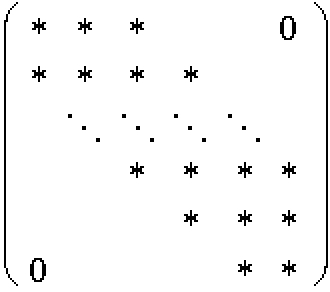
\includegraphics[width=5cm]{images/band.jpg}  
    \end{image}
    
    
  \item große Matrizen (mit zusätzlichen Eigenschaften)\\
    $\rightarrow$ \textbf{iterative Methoden:} kenne Startwert
    $x_0$, berechne neue Approximation $x_i$ unter
    Ausnutzung der vorherigen bis die
    \textbf{Näherungslösung} $x_i$ \enquote{gut genug ist}.
  \end{itemize}
  
\item \textbf{Lineare Ausgleichsprobleme}\\
  Beispiel:\\
  Wir messen den Zusammenhang zwischen Spannung U und
  Stromstärke I
\begin{image}{Einfacher Stromkreis}
  \parbox[c]{3cm}{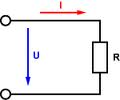
\includegraphics[width=2cm]{images/ohmsche.jpeg} }
\end{image}
\begin{image}{Linearausgleich von Messwerten}
  \parbox[c]{6cm}{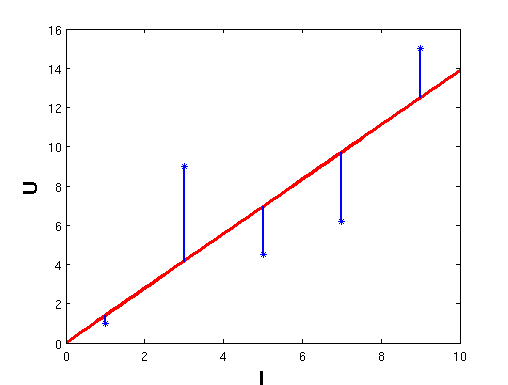
\includegraphics[width=5cm]{images/linausgl2.png}}
\end{image}
  Ohmsches Gesetz: $U = R \cdot I$\\
  Gesucht ist der Widerstand R. \\
  ($U_i, I_i$) seien die Messdaten mit möglichen Messfehlern.\\
  Finde nun $R$, sodass 
  $\; f(R)\, =\,  \min\limits_r \; \sum\limits_i \; (U_i - r \; I_i)^2$
  
\item \textbf{Lösung nichtlinearer Gleichungen},
  z.B.
  \begin{itemize}
  \item Berechnung von Nullstellen $g(x) = 0$
  \item Berechnung von Fixpunkten $f(x) = x$
  \end{itemize}  
\item \textbf{Eigenwertwertberechnung}
  $\quad Ax= \lambda x, \qquad \; \lambda \in \mathbb{C}$
  
  
\item \textbf{Interpolation}\\
  Setze Meßdaten zu einer kontinuierlichen Funktion fort, \\
  aber wie \enquote{glatt}?\\
  z.B. stückweise konstant, stückweise linear, oder 
  falls sie
  eine Schwingung repräsentieren, berechne die zugehörige
  Fourierreihe  
  
\item \textbf{Berechnung von Integralen} (Quadraturformeln) \\ 
  Approximation von $\int_a^b \; f(x) \; dx$
\end{enumerate}~\\

Bei allem spielt die \textbf{Fehleranalyse} eine große Rolle und
ihre Grundbegriffe werden in einem extra Abschnitt behandelt.

%%% Local Variables:
%%% mode: latex
%%% TeX-master: "../numerik_script"
%%% End:


% Kap. 2: Lineare Gleichungssysteme: Direkte Methoden
% % % % % % % % % % % % % % 
% 
% Skript zu NUMERIK I
% WS14/15
% von Prof. Dr. Blank
% Universität Regensburg
% 
% 
%	Kap. 2: Lineare Gleichungssysteme: Direkte Methoden
% 
% % % % % % % % % % % % % % 


\chapter{Lineare Gleichungssysteme: Direkte Methoden}
Sei $ A \in \R^{n\times n}$, $b \in \R^n$. Gesucht ist $x\in \R^n$ mit 
\begin{gather*}
  A\cdot x = b
\end{gather*}
Weitere Voraussetzungen sind die Existenz und Eindeutigkeit einer
Lösung.

Bemerkungen hierzu:
\begin{itemize}
\item Ein verlässlicher Lösungsalgorithmus überprüft dies und behandelt alle Fälle. 
\item Die Cramersche Regel ist ineffizient (s. Einführung
  \ref{CramerscheRegel}).
\item Das Inverse für $x=A^{-1}\cdot b$ aufzustellen ist ebenso ineffizient,
  denn es ist keine Lösung für alle $b\in \R^n$ verlangt
  und der Algorithmus wird evtl. instabil aufgrund vieler Operationen.
\item [$\Rightarrow$] Invertieren von Matrizen vermeiden!!
\item [$\Rightarrow$] Lösen des Linearen Gleichungssystems!!
\end{itemize}

\sectione{Gaußsches Eliminationsverfahren} \label{2.2.1}
\index{Gaußsches Eliminationsverfahren}\index{Dreieckszerlegung}
Das Verfahren wurde 1809 von Friedrich Gauß,
1759 von Josepf Louis Lagrange beschrieben
und war seit dem 1. Jhd. v. Chr. in China bekannt.

\subsectione{Vorwärtselimination} \label{2.1.1}
\index{Vorwärtselimination}\index{Vorwärtssubstitution}
Das Gaußverfahren gilt der Lösung eines linearen Gleichungssystems der Form
\begin{align*}
  Ax &= b
\end{align*}
mit $A=(a_{ij})_{i,j \leq n} \in K^{n\times n}$ Matrix und $b=(b_i)_{i\leq n} \in K^n$ Vektor.\\
Der zugehörige Algorithmus sieht folgendermaßen aus:
\begin{gather*}
  \begin{array}{ccccccccc}
    a_{11}x_1 &+& a_{12}x_2 &+& \cdots &+& a_{1n}x_n & = & b_1 ~~\\
    a_{21}x_1 &+& a_{22}x_2 &+& \cdots &+& a_{2n}x_n & = & b_2 \\
    \vdots         &&        \vdots     &&              &&   \vdots       &    & \vdots \\
    a_{n1}x_1 &+& a_{n2}x_2 &+& \cdots &+& a_{nn}x_n & = & b_n \\\\
              &&&& \Downarrow &&&& 
  \end{array} \\
  \quad	(\text{$i$-te Zeile}) - (\text{1. Zeile})\cdot \frac{a_{i1}}{a_{11}} \Rightarrow a_{i1}=0\\
  \begin{array}{ccccccccc}
    &&&& \Downarrow &&&&  \\\\
    a_{11}x_1 &+& a_{12}x_2 &+& \cdots &+& a_{1n}x_n & = & b_1 \\
    &+& a_{22}^{(1)}x_2 &+& \cdots &+& a_{2n}^{(1)}x_n & = & b_2^{(1)} \\
    &&        \vdots     &&              &&   \vdots       &    & \vdots \\
    && && && a_{nn}^{(1)}x_n & = & b_n^{(1)} \\\\
    &&&& \Downarrow &&&&\\
    &&&& \vdots &&&&
  \end{array} 
\end{gather*}
mit
\begin{align*}
  a_{ij}^{(1)} &= a_{ij}-a_{1j}\cdot \frac{a_{i1}}{a_{11}}
  & \text{für }i,j = 2, \cdots, n \\
  b_i^{(1)}      &= b_i- b_1\cdot \frac{a_{i1}}{a_{11}}
  & \text{für }i = 2, \cdots, n 
\end{align*}

% --------------------------------------------------------

In jedem Schritt werden die Einträge der $k$-ten Spalte analog 
unterhalb der Diagonalen (also $k=1, \cdots, n-1$) eliminiert:
\marginpar{08.10.2014}
\begin{align*}
  (\text{$i$-te Zeile})- (\text{$k$-te Zeile})\cdot\frac{a_{ik}}{a_{kk}}
  && \text{für } i=k+1, \cdots ,n 
\end{align*}
Die Reihe 
\begin{gather*}
  A \rightarrow A^{(1)} \rightarrow A^{(2)} \rightarrow \dotsm \rightarrow A^{(n-1)}
\end{gather*}
wird bis zum $n$-ten Schritt fortgeführt, d.h. bis eine obere Dreiecksgestalt eintritt:
\begin{align}
  \nonumber
  \underbrace{	\begin{pmatrix}
      a_{11} & \dotsm & \dotsm & a_{1n} \\
      & a_{22}^{(1)} & \dotsm & a_{2n}^{(1)} \\
      &&              \ddots  &  \vdots \\
      0        && &                             a_{nn}^{(n-1)}
    \end{pmatrix}}_{\coloneqq R}
                    \cdot
                    \begin{pmatrix}
                      x_1 \\
                      x_2 \\
                      \vdots \\
                      x_n
                    \end{pmatrix}
             & =
               \underbrace{\begin{pmatrix}
                   b_1 \\
                   b_2^{(1)} \\
                   \vdots \\
                   b_n^{(n-1)}
                 \end{pmatrix}}_{\coloneqq z} \\
  Rx &= z 	\label{II.1.1} 
\end{align}
wobei für  $i=k+1, \cdots ,n$ die Einträge wie folgt aussehen:
\begin{align}	
  l_{ik} &\coloneqq \frac{a_{ik}^{(k-1)}}{a_{kk}^{(k-1)}} \label{II.1.2} \\
  a_{ij}^{(k)} &= a_{ij}^{(k-1)} - a_{kj}^{(k-1)}\cdot l_{ik} \label{II.1.3}
               & \text{für } j=k+1, \cdots , n\\ %
  b_i^{(k)} &= b_i^{(k-1)} -b_k^{(k-1)} \cdot   l_{ik}
              \label{II.1.4}\index{Vorwärtssubstitution}
\end{align}
Dieser Prozess wird \textbf{Vorwärtselimination} genannt.\\

Der zugehörige Algorithmus ist:

\begin{pseudocode}{0.5\linewidth}
  \textbf{for} $ k = 1, \ldots , n-1$\\
  |~	\> \textbf{for} $i = k + 1, \ldots , n$ \\
  |~	\> |~\> $l_{ik} = a_{ik} /a_{kk}$\\
  |~	\> |~\> \textbf{for} $j = k + 1, \ldots , n$ \\
  |~	\> |~\>|~\> $a_{ij} = a_{ij} - l_{ik} a_{kj} $\\
  |~	\> |~\> \textbf{end}\\
  |~	\> |~\> $b_i = b_i -  l_{ik} b_k $\\
  |~	\> \textbf{end} \\
  \textbf{end}
\end{pseudocode}

\subsectione{Rückwärtselimination}\label{2.1.2}
Für die Lösung des Gleichungssystems ist dann noch die
\textbf{Rückwärtssubstitution} \index{Rückwärtssubstitution} nötig:
\begin{align}
  x_n &= \frac{b_n^{(n-1)}}{a_{nn}^{(n-1)}} \label{II.1.5} \\
  x_{n-1} &=  \frac{b_{n-1}^{(n-2)}-a_{n-1,n}^{(n-1)}\cdot x_n}
            {a_{(n-1)(n-1)}^{(n-2)}} \label{II.1.6} \\
  x_k &= \frac{b_k^{(k-1)}-\sum_{j=k+1}^{n}a_{kj}^{(k-1)}x_j}
        {a_{kk}^{(k-1)}} \label{II.1.7}
\end{align}

Als Algorithmus:

\begin{pseudocode}{0.5\linewidth}
  \textbf{for} $k = n, n -1, \ldots , 1$ \\
  |~		\>$x_k = b_k$ \\
  |~		\>\textbf{for} $j = k + 1, \ldots , n$ \\
  |~		\>|~	$x_k = x_k - a_{kj}x_j$ \\
  |~		\>\textbf{end} \\
  |~		\>$x_k = x_k /a_{kk}$ \\
  \textbf{end}
\end{pseudocode}~\\

% \subsectione{Vorsicht}
\begin{Beme}
  Algorithmen \ref{2.1.1} und \ref{2.1.2} sind nur ausführbar,
  falls für die sog. \textbf{Pivotelemente $\mathbf{a_{kk}^{(k-1)}}$ } \index{Pivotelement} gilt:
  \begin{gather*}
    a_{kk}^{(k-1)} \neq 0 \quad   \text{für } k=1, \cdots , n
  \end{gather*}
  Dies ist auch für invertierbare Matrizen nicht immer gewährleistet.
\end{Beme}


\subsectione{Weitere algorithmische Anmerkungen}	\label{2.1.4}
Matrix $A$ und Vektor $b$ sollten möglichst \textbf{nie} überschrieben werden!
(Stattdessen kann eine Kopie überschrieben werden.)
Das Aufstellen von $A$ und $b$ ist bei manchen Anwendungen das teuerste,
sie gehen sonst verloren.
In \ref{2.1.1} wird das obere Dreieck von $A$ überschrieben.
Dies ist möglich, da in \eqref{II.1.3} nur die Zeilen $k+1, \cdots, n$
mithilfe der $k$-ten bearbeitet werden. 
Am Ende steht $R$ im oberen Dreieck von $A$ und $z$ in $b$.
Die $l_{ik}$ werden spaltenweise berechnet und können daher
anstelle der entsprechenden Nullen (in der Kopie) von $A$ gespeichert werden, d.h.:
\begin{gather}
  \widetilde{L} \coloneqq (l_{ik})  \label{II.1.8}
\end{gather}
und $R$ werden sukzessive in A geschrieben. 
\begin{gather*}
  \begin{pmatrix}
    \hspace{0.15cm}
    \begin{tikzpicture}[scale=5.7,line cap=round,line join=round,>=triangle 45,x=1.0cm,y=1.0cm]
      \draw[color=black] (0,0) -- (0,0.9) -- (0.9,0) -- cycle;
      \draw[color=black] (0.28,0.35) node {$l_{ij}$};
      \draw[color=black] (1.05,0) -- (1.05,1.05) -- (0,1.05) -- cycle;
      \draw[color=black] (0.72,0.65) node {$r_{ij}$};
    \end{tikzpicture}
    \hspace{0.15cm}
  \end{pmatrix}\hspace{0.5cm}
  \begin{pmatrix}
    \hspace{0.15cm}
    \begin{tikzpicture}[scale=3,line cap=round,line join=round,>=triangle 45,x=1.0cm,y=1.0cm]
      \draw (0,1.8) rectangle (2,2);
      \draw (1,1.9) node {1};
      %	
      \draw (0.2,1.5) rectangle (0,1.7);
      \draw (0.1,1.6) node {2};
      %	
      \draw (0.3,1.5) rectangle (2,1.7);
      \draw (1.15,1.6) node {3};
      %	
      \draw (0,0) rectangle (0.2,1.4);
      \draw (0.1,0.7) node {4};
      %	
      \draw (0.3,1.2) rectangle (0.5,1.4);
      \draw (0.4,1.3) node {5};
      %	
      \draw (0.6,1.2) rectangle (2,1.4);
      \draw (1.3,1.3) node {6};
      %	
      \draw (0.3, 0) rectangle (0.5,1.1);
      \draw (0.4,0.55) node {7};
      %	
      \draw (0.6,0) rectangle (2,1.1);
    \end{tikzpicture}
    \hspace{0.15cm}
  \end{pmatrix}
\end{gather*}
Der Vektor $z$ und anschließend der Lösungsvektor $x$
kann in (eine Kopie von) $b$ geschrieben werden.
Wird eine neue rechte Seite $b$ betrachtet,
muss \ref{II.1.1} nicht komplett neu ausgeführt werden,
da sich $\widetilde{L}$ nicht ändert. Es reicht \ref{II.1.4} zu wiederholen.

\begin{Defe}
  \label{2.1.5}
  \index{Dreieckszerlegung}
  Die \textbf{Dreieckszerlegung} einer Matrix $A$
  entspricht dem Verfahren aus \ref{2.1.1}, nur ohne die Zeile \eqref{II.1.4}.
\end{Defe}

\begin{Defe}
  \index{Vorwärtssubstitution}
  Die \textbf{Vorwärtssubstitution} entspricht der in \ref{2.1.4}
  bzw. dem Verfahren aus \ref{2.1.1} 
  ohne die Bestimmung von $l_{ik}$ und $R$, also nur Schritt \eqref{II.1.4}.
\end{Defe}

\subsectione{Algorithmus: Gauß-Elemination zur Lösung von $Ax=b$}\index{Gauß-Eleminator}
\begin{framed}
  \begin{enumerate}[1]
  \item Dreieckszerlegung
  \item Vorwärtssubstitution        $\quad b_i^{(k)} = b_i^{(k-1)} -b_k^{(k-1)} \cdot   l_{ik} $
  \item Rückwärtssubstitution      $\quad x_k = \frac{b_k^{(k-1)}-\sum_{j=k+1}^{n}a_{kj}^{(k-1)}x_j}{a_{kk}^{(k-1)}}$
  \end{enumerate}
\end{framed}

\subsectione{Rechenaufwand gezählt in \enquote{flops}} 
\index{flops}\index{floating point operations}\index{Rechenaufwand}
\index{Dreieckszerlegung!Rechenaufwand}
\index{Vorwärtssubstitution!Rechenaufwand}
\index{Rückwärtssubstitution!Rechenaufwand}
\textbf{\enquote{flops} }= \textbf{fl}oating point \textbf{op}eration\textbf{s}
\begin{enumerate}
\item[\textbf{1.}] \textbf{Dreieckszerlegung} 
  \begin{tabbing}
    für $j=k+1, \ldots, n\quad$ \= 1 Addition, 1 Multiplikation für
    $a_{ij}$ \\
    für $i=k+1, \ldots, n$ \> 1 Division zusätzl. für $ l_{ik}$
  \end{tabbing}
  Dies ist je für $k=1, \ldots, n-1$, also ist die Zahl an Additionen und Multiplikationen
  \begin{align*}
    \sum_{k=1}^{n-1}(n-k)^2 &= \sum_{k=1}^{n-1}k^2 \\
                            &= \frac{(n-1)n(2n-1)}{6} \\
                            &= \frac{2n^3-3n^2+n}{6}\, .
  \end{align*}
  Für große $n$ sind das etwa $\frac{n^3}{3}$ Additionen und Multiplikationen und
  \begin{gather*}
    \sum_{k=1}^{n-1} (n-k) = \frac{n^2-n}{2} \approx \frac{n^2}{2}
  \end{gather*}
  Divisionen.
  Damit ergibt sich eine Gesamtanzahl an flops von
  \begin{gather*}
    2\cdot\frac{2n^3-3n^2+n}{6} + \frac{n^2-n}{2} 
    = \frac{2}{3} n^3 - \frac{1}{2}n^2 - \frac{1}{6} n
    \approx \frac{2}{3}n^3
  \end{gather*}
  für große $n$.
  
\item[\textbf{2.}] \textbf{Vorwärts- bzw. Rückwärtssubstitution}  \\
  Hier ergeben sich je
  $\sum_{k=1}^{n-1} (n-k) = \frac{n^2-n}{2} \approx \frac{n^2}{2}$
  Multiplikationen und Additionen sowie 
  $n$ Divisionen für die Rückwärtssubstitution und damit insgesamt $n^2+n$ flops.	
\end{enumerate}
\paragraph{Zusammenfassung}~ \\
Die Dreieckszerlegung benötigt $\mathcal{O}(n^3)$ flops und 
die Vorwärts- bzw. Rückwärtssubstitution $\mathcal{O}(n^2)$ flops.


\begin{Defe}[Landau-Symbole]
  \index{Landau-Symbole}
  Seien $f,g : D\longrightarrow \R, D\subset \R, -\infty\leq a\leq \infty$ und
  $(a_n)_{n\in\N}, (b_n)_{n\in\N}$ Folgen in $\R$.
  \begin{enumerate}[a)]
  \item $f(x) = \mathcal{O}(g(x))$ für $x\longrightarrow a$, falls
    \begin{gather*}
      \exists U(a),c\in\R\colon\forall x\in U(a)\colon |f(x)|\leq c\cdot |g(x)|
    \end{gather*}
    (bzw. falls $\lim\limits_{x\to a}\frac{|f(x)|}{|g(x)|} \leq c$)
  \item $f(x) = o(g(x))$ für $x\longrightarrow a$, falls 
    $\lim\limits_{x\rightarrow a}\frac{|f(x)|}{|g(x)|} = 0$
  \item $a_n = \mathcal{O}(b_n)$ für $n\longrightarrow \infty$, falls
    \begin{gather*}
      \forall\varepsilon>0\colon\exists N\in\N\colon
      \forall n\geq N\colon|a_n|\leq\varepsilon |b_n|
    \end{gather*}
  \end{enumerate}
\end{Defe}

\subsectione{Allgemeines zur Aufwandsbetrachtung}\index{Rechenaufwand}
Die Anzahl der Rechenoperationen ist nicht immer ausschlaggebend für
den Aufwand, z.B.
\begin{description}
\item[Parallelrechner:] 
  In manchen Algorithmen sind Rechenschritte parallel ausführbar.
  Damit entspricht die Zeit nicht der Anzahl an Operationen und es wird zusätzliche
  \enquote{Kommunikationszeit} benötigt.
\item[Sortieralgorithmen:] Die Indexverwaltung benötigt Zeit, aber keine/kaum Rechenoperationen
\item[If-When-Abfragen:] entsprechend
\end{description}
Rechenoperationen liefern jedoch oft eine gute Schätzung.

% -----------------------------------------------------------------

\subsectione{Formalisieren des Gauß-Algorithmus: LR-Zerlegung}
\marginpar{13.10.2014}
\index{Gaußsches Eliminationsverfahren} \index{LR-Zerlegung}
\begin{enumerate}[a)]
\item \textbf{Rückwärtssubstitution:}\index{Rückwärtssubstitution!formal}  
  entspricht $Rx=z$
\item \textbf{Vorwärtssubstitution:}\index{Vorwärtssubstitution!formal} 
  \begin{align*}
    b^{(k)}_i&=b_i^{(k-1)}-l_{ik}b_k^{(k-1)} && i=k+1, \dotsc , n\\
    b^{(k)} &= b^{(k-1)}-l_kb_k^{(k-1)} 
                                             && \text{mit }l_k\coloneqq 
                                                \begin{pmatrix}
                                                  0&\dotsm&0&l_{k+1,k}&\dotsm&l_{n,k}
                                                \end{pmatrix}^T
  \end{align*}
  Sei $e_k\in\R^n$ der $k$-te Einheitsvektor und 
  \begin{gather}
    L_k \coloneqq I- l_ke_k^T = \begin{pmatrix}
      1&&&&&&\\
      0&\ddots&&&0\\
      \\
      &&1\\
      \vdots&&-l_{k+1,k}&1\\
      &&\vdots&&\ddots \\
      &&-l_{n,k}&&&1
    \end{pmatrix}
    \label{II.1.9}
  \end{gather}
  dann gilt $b^{(k)} =L_kb^{(k-1)}$, also
  \begin{gather*}
    z = L_{n-1}\cdot L_{n-2} \cdot \ldots \cdot L_1b
  \end{gather*}
  Sei
  \begin{gather}
    L\coloneqq L_1^{-1} \cdot \ldots \cdot L_{n-1}^{-1}
    \label{II.1.10}
  \end{gather}
  Hiermit folgt dann, dass die Vorwärtssubstitution
  \begin{gather}
    Lz=b\label{II.1.11}
  \end{gather}
  enspricht.
\item \textbf{Dreieckszerlegung:}\index{Dreieckszerlegung!formal}
  Wie für die Vorwärtssubstitution ergibt sich
  \begin{gather*}
    A^{(k)}=L_kA^{(k-1)}
  \end{gather*}
  und somit $R=L_{n-1}A^{(n-2)}= L_{n-1}\ldots L_1A $ bzw.
  \begin{gather} 
    A=L\cdot R
    \label{II.1.12}
  \end{gather}
\end{enumerate}


\begin{Leme}\label{2.1.12}\index{Frobeniusmatrix}~
  \begin{enumerate}[1.]
  \item $L_k$ ist eine Frobeniusmatrix, d.h. sie unterscheidet sich höchstens
    in einer Spalte von der Einheitsmatrix $I$.
  \item $L_k^{-1} = I + l_ke_{k}^T$
  \item Es gilt:
    \begin{align}
      L &= L_1^{-1} \cdot \dotsc \cdot L_{n-1}^{-1}  
          \label{II.1.13}
      \\ \nonumber
        & = I + \sum_{i=1}^{n-1} l_i e_i^T \\ \nonumber
        &= \begin{pmatrix}
          1 && 0 ~ \\
          &\ddots& \\
          ~l_{ij} && ~1
        \end{pmatrix} \\ \nonumber
        &= I+ \widetilde{L}
    \end{align}
  \end{enumerate}
\end{Leme}
Hiermit ergibt sich der folgende Satz: 

% \subsectione{Satz (LR- oder LU-Zerlegung)} \index{LR-Zerlegung}\index{LU-Zerlegung}
\begin{Satze}[LR- oder LU-Zerlegung]
  Das obige Verfahren (\eqref{II.1.2} und \eqref{II.1.3}) erzeugt unter der Voraussetzung
  von nicht-nullwertigen Pivotelementen eine Faktorisierung
  \begin{align*}
    A= L\cdot R 
  \end{align*}
  wobei $R$ eine obere Dreiecksmatrix und $L$ eine untere, normierte Dreiecksmatrix ist,
  d.h. für $i=1, \cdots , n$ gilt $l_{ii}= 1$. \\
  Weiterhin existiert zu jeder regulären Matrix höchstens eine solche Zerlegung.
\end{Satze}

\begin{proof}
  Zur Eindeutigkeit:
  \begin{gather*}
    A=LR \Leftrightarrow a_{ij}=\sum_{k=1}^{\min{j,k}}l_{ik}r_{kj}
  \end{gather*}
  Da $l_{ii}=1$ gilt, folgt
  \begin{align*}
    r_{ij}&=a_{ij}-\sum_{k=1}^{i-1}l_{ik}r_{kj}  &&\text{für }i\leq j\quad\text{und}\\
    l_{ij}&=\frac{1}{r_{ij}}\left( 
            a_{ij}-\sum_{k=1}^{j-1}l_{ik}r_{kj}
            \right)
                                                 &&\text{für }i>j,
  \end{align*}
  da mit $A$ auch $R$ regulär (=invertierbar) ist, und somit $\det(A)=\prod_{j=1}^{n}\neq 0$, also $ r_{jj}\neq 0$ gilt.
  Diese können rekursiv, also eindeutig, berechnet werden,
  wenn auch die Reihenfolge der Berechnung nicht eindeutig ist.
  Mögliche Verfahren sind z.B. das \textbf{Verfahren von Crout}\index{Verfahren von Crout}
  \begin{gather*}
    \begin{pmatrix}
      \begin{tikzpicture}[scale=4,line cap=round,line join=round,>=triangle 45,x=1.0cm,y=1.0cm]
        \draw (0,1.8) rectangle (2,2);
        \draw (1,1.9) node {1};
        % 
        \draw (0,0) rectangle (0.2,1.7);
        \draw (0.1,0.85) node {2};
        % 
        \draw (0.3,1.5) rectangle (2,1.7);
        \draw (1.15,1.6) node {3};
        % 
        \draw (0.3,0) rectangle (0.5,1.4);
        \draw (0.4,0.7) node {4};
        % 
        \draw (0.6,1.2) rectangle (2,1.4);
        \draw (1.3,1.3) node {5};
        % 
      \end{tikzpicture}
    \end{pmatrix}
  \end{gather*}
  
  oder eckweise
  \begin{gather*}
    \begin{pmatrix}
      \begin{tikzpicture}[scale=4,line cap=round,line join=round,>=triangle 45,x=1.0cm,y=1.0cm]
        \draw (0,1.8) -- (0.2,1.8) -- (0.2,2);
        \draw (0.1,1.9) node {1};
        % 
        \draw (0,1.5) -- (0.5,1.5) -- (0.5,2);
        \draw (0.35,1.65) node {2};
        % 
        \draw (0,1.2) -- (0.8,1.2) -- (0.8,2);
        \draw (0.65,1.35) node {3};
        % 
        \draw[color = white] (2,2) -- (2,0);
      \end{tikzpicture}
    \end{pmatrix}
  \end{gather*}
  
  oder zeilenweise
  \begin{gather*}
    \begin{pmatrix}
      \begin{tikzpicture}[scale=4,line cap=round,line join=round,>=triangle 45,x=1.0cm,y=1.0cm]
        \draw (0,1.8) rectangle (2,2);
        \draw (1,1.9) node {1};
        % 
        \draw (0,1.5) rectangle (0.2,1.7);
        \draw (0.1,1.6) node {2};
        % 
        \draw (0.3,1.5) rectangle (2,1.7);
        \draw (1.15,1.6) node {3};
        % 
        \draw (0,1.2) rectangle (0.5,1.4);
        \draw (0.25,1.3) node {4};
        % 
        \draw (0.6,1.2) rectangle (2,1.4);
        \draw (1.3,1.3) node {5};
        % 
        \draw (0,0.9) rectangle (0.8,1.1);
        \draw (0.4,1) node {6};
        % 
        \draw (0.9,0.9) rectangle (2,1.1);
        \draw (1.45,1) node {7};
        % 
        \draw[color=white] (0,0) -- (2,0);
      \end{tikzpicture}
    \end{pmatrix}
  \end{gather*}
  oder wie in \ref{2.1.1}.
\end{proof}

\sectione{Gaußsches Eliminationsverfahren mit Pivotisierung}
\paragraph{Beispiel} Die Matrix $A= \begin{pmatrix}0&1\\1&0\end{pmatrix} $
ist invertierbar, aber die Gauß-Elimination versagt. 
Permutiere also die erste mit der
zweiten Zeile und der Algorithmus wird anwendbar.
\paragraph{Allgemein} Vermeide die Division durch betragsmäßig kleine Zahlen! 

\subsectione{Spaltenpivotisierung}
\index{Pivotisierung}%
\index{Pivotisierung!halbmaximale}\index{Pivotisierung!partielle}%
\index{Pivotisierung!Spalten-}%
Eine Spaltenpivotisierung, auch partielle oder halbmaximale Pivotisierung,
erfolgt, indem im $k$-ten  Eliminationsschritt durch Zeilenvertauschen
das größte Spaltenelement das Pivotelement stellt:
\begin{image}{Ein Schritt der Spaltenpivotisierung}
  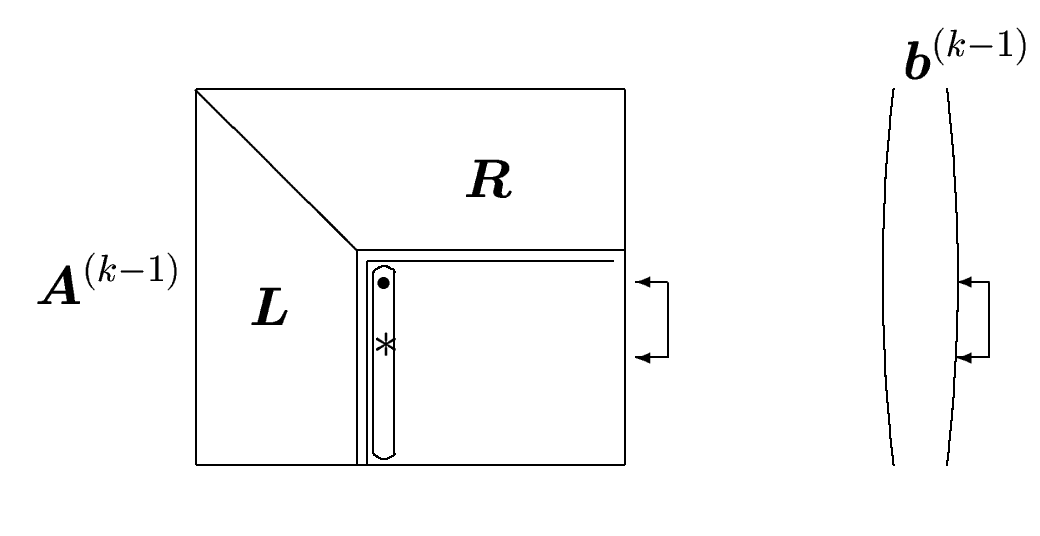
\includegraphics[width=0.5\linewidth]{images/Gausspivot.png}
\end{image}

\begin{enumerate}[1.]
\item Bestimme das Pivotelement $a_{pk}^{(k-1)}$ 
  als betragsmäßig größtes der \enquote{Rest-Spalte}, d.h.
  \begin{gather*}
    |a_{pk}^{(k-1)}|\geq |a_{jk}^{(k-1)}| \qquad  \text{ für } j=k,\ldots , n
  \end{gather*}
\item Vertausche in $A^{(k-1)}$ die $k$-te mit der $p$-ten Zeile
\item Führe einen Gauß-Eliminationsschritt aus.
\end{enumerate}

\begin{Beme}~
  \begin{enumerate}[a)]
  \item Hiermit gilt $|l_{jk}| \ll 1$.
  \item Anstelle von Spaltenpivotisierung kann eine \textbf{Zeilenpivotisierung}\index{Pivotisierung!Zeilen-}
    durchgeführt werden.
    Welche günstiger (in cpu-time) ist, hängt von der Rechnerarchitektur und
    der damit zusammenhängenden Umsetzung des Gauß-Algorithmus ab.\\
    (Beispielsweise greifen Vektorrechner entweder auf die gesamte Spalte
    oder auf die gesamte Zeile einer Matrix zu und bevorzugen dementsprechend
    Operationen spalten- bzw. zeilenweise.)
  \item Der Aufwand enthält (bis auf $|\cdot |$) keine Rechenoperationen (flops),
    aber $\mathcal{O}(n^2)$ Vergleiche und Vertauschungen.
  \item Eine \textbf{vollständige Pivotsuche}\index{Pivotisierung!vollständige} sucht das betragsmäßig größte Element der gesamten Restmatrix und benötigt $\mathcal{O}(n^3) $ Vergleiche
    (sie wird so gut wie nie angewendet).
  \end{enumerate}
\end{Beme}

Damit die LR-Zerlegung unabhängig von der rechten Seite erstellt werden kann, müssen die Permutationen gespeichert werden.
Hierfür verwendet man  einen sog. \textbf{Permutationsvektor} $\Pi$, wobei
\begin{gather*}
  \Pi^{(k-1)}(r) = s
\end{gather*}
bedeutet, dass nach dem $(k-1)$-ten Eliminationsschritt in der $r$-ten Zeile
von $A^{(k-1)}$ die $s$-te bearbeitete Zeile von $A$ steht, also
\begin{align*}
  \Pi^{(k)}(k) &= \Pi^{(k-1)}(p) \\
  \Pi^{(k)}(p) &= \Pi^{(k-1)}(k)  \quad \text{und entsprechend} \\
  \scriptsize \Pi^{(k)} (i) &= \Pi^{(k)} (i) \quad \text{ für }  i\neq k,p 
\end{align*}
Für die \textbf{Permutationsmatrix}\index{Permutationsmatrix}
$P_{\Pi}$ gilt: 
\begin{align*}
  P_{\Pi}&\coloneqq (e_{\Pi(1)}, \ldots , e_{\Pi(n)}) 
  & e_j\coloneqq 
    {\scriptsize\begin{pmatrix}0\\\vdots\\0\\1\\0\\\vdots\\0\end{pmatrix}
  \begin{array}{l}\\\\\shortleftarrow \text{$j$-te Stelle}\\\\\\\end{array}}\\
  PA&= LR \\
  P^{-1} &= P^T
           \det P_{\Pi} = \Sign(\Pi) 
           % \\
           % &=  \begin{cases}
           %   +1&  \text{falls }\Pi \text{ von gerader}\\
           %   -1 &  \text{falls } \Pi \text{ von ungerader}
           % \end{cases} \text{ Anzahl an Transpositionen erzeugt wird}
\end{align*}


\subsectione{Algorithmus: Gauß-Elimination mit Spaltenpivotisierung}\label{2.2.3}
Der zugehörige Algorithmus zur Spaltenpivotisierung ist: \\

\begin{pseudocode}{0.9\linewidth}
  $\pi(1 : n) = [1 : n] $  \\
  \textbf{for} $k = 1, \dots, n-1$ \\
  ~|	  \> bestimme Pivotzeile $p$, so dass\\
  ~|	  \>\>	$|a_{pk} | = \max\{|a_{jk} | , j = k, . . . , n\}$ \\
  ~|	  \> $\pi(k) \leftrightarrows\footnotemark \pi(p)$ \\
  ~|	  \> $A(k, 1 : n) \leftrightarrows A(p, 1 : n)$ \\
  ~|	  \> \textbf{if} $a_{kk} \neq 0$ \\
  ~|	  	   \>~|\> $zeile = [k + 1 : n]$ \\
  ~|	  	   \>~|\> $A(zeile, k) = A(zeile, k)/a_{kk}$ \\
  ~|	  	   \>~|\> $A(zeile, zeile) = A(zeile, zeile) - A(zeile, k)A(k, zeile)$\\
  ~|	  \> \textbf{else} \\
  ~|	  	   \>~|\> \enquote{$A$ ist singulär}\\
  ~|	  \> \textbf{end}\\
  \textbf{end}
\end{pseudocode}	\footnotetext{$\leftrightarrows$ bedeutet \enquote{vertausche mit}}
\\

\begin{Satze}[Dreieckszerlegung mit Permutationsmatrix] \label{2.2.4} 
  Für jede invertierbare Matrix $A$ existiert eine Permutationsmatrix $P$,
  so dass eine Dreieckszerlegung
  \begin{gather*}
    PA = LR
  \end{gather*}
  existiert.
  $P$ kann so gewählt werden, dass alle Elemente von $L$ betragsmäßig kleiner oder gleich
  1 sind, d.h.
  \begin{gather*}
    |l_{ij}| \leq 1\quad \forall i, j
  \end{gather*}
\end{Satze}


\begin{proof}
  Da $\det A \neq 0$ ist, existiert eine Transposition $\tau_1$, s.d. 
  \begin{gather*}a_{11}^{(1)}= a_{\tau_1, 1} \neq 0 \end{gather*}
  und
  \begin{gather*}
    | a_{\tau_1, 1} | \geq |a_{i1}| 
    \quad \forall i=1, \cdots, n \, . 
  \end{gather*}
  Wir erhalten damit
  \begin{gather*}
    L_1P_{\tau_1} \cdot A = A^{(1)} = \begin{pmatrix}
      a_{11}^{(1)} && \cdots ~&  ~\\
      0 \\
      \vdots && B^{(1)} \\
      0
    \end{pmatrix}
  \end{gather*}
  und alle Elemente von $L_1 $ sind betragsmäßig kleiner oder gleich 1 sowie
  $\det L_1 = 1 $. \\
  Daraus folgt
  \begin{align*}
    \det B^{(1)} & = \frac{1}{\underbrace{a_{11}^{(1)}}_{\neq 0}} \cdot \det A^{(1)} \\
                 & = \frac{1}{a_{\tau_1, 1}^{(1)}}\cdot \det (L_1) \cdot \det (A) \\
                 & \neq 0 \, .
  \end{align*}
  Also ist $B^{(1)}$ invertierbar. \\
  
  Induktiv erhalten wir dann
  \begin{gather*}
    R = A^{(n-1)} = L_{n-1}P_{\tau_{n-1}} \cdot \dotsc \cdot L_1 P_{\tau_1} \cdot A
  \end{gather*}\\
  
  % ------------------------------------------------------

  Da $\tau_i$ nur zwei Zahlen $\geq i $ vertauscht, ist
  \marginpar{15.10.2014}
  \begin{align*}\index{Vorwärtselimination}
    \Pi_i  &\coloneqq \tau_{n-1} \circ \ldots \circ \tau_i \quad\text{ für } i=1,\ldots (n-1) 
  \end{align*}
  eine Permutation der Zahlen $\{i,\dots, n\}$, d.h. insbesondere gilt:
  \begin{alignat*}{2}
    \Pi_i(j)&=j  & \quad &\text{ für } j=1,\dots,(i-1) \\
    \Pi_i(j)&\in \{i, \dots, n\} & &\text{~für~}j=i,\dots, n\,. 
  \end{alignat*}
  \begin{align*}
    P _{\Pi_{i+1}}  &= (e_1, \dotsc e_i, e_{\Pi_{i+1}(i+1)}, \dotsc, e_{\Pi_{i+1}(n)}) 
                      = \begin{pmatrix}
                        I_i & 0 \\
                        0 & P_{\sigma}
                      \end{pmatrix}
  \end{align*}
  Damit folgt:
  \begin{align*}
    P_{\Pi_{i+1}}\cdot L_i\cdot P_{\Pi_{i+1}}^{-1}
    &= P_{\Pi_{i+1}} \cdot 
      \left(\begin{array}{ccc|ccc}
              & I_i & && 0 & \\
              \cline{1-6}
              & & -l_{i+1, i} & & & \\
              &  0 &  \vdots  & & I_{n-i} &\\
              &    & -l_{n, i} & &  & 
            \end{array}\right)
                                      \cdot\begin{pmatrix}
                                        I_i & 0 \\
                                        0 & P_{\sigma}^{-1}
                                      \end{pmatrix}\\
    &= \begin{pmatrix}
      I_i & 0 \\
      0 & P_{\sigma}
    \end{pmatrix}
          \cdot   \ldots  \cdot
          \left(\begin{array}{ccc|ccc}
                  & I_i & && 0 & \\
                  \cline{1-6}
                  \cdot & & -l_{i+1, i} & & & \\
                  &  0 &  \vdots      & & P_{\sigma}^{-1} &\\
                  &     & -l_{n, i} & &  & 
                \end{array}\right) \\
    &= \left(\begin{array}{ccc|ccc}
               & I_i & && 0 & \\
               \cline{1-6}
               &     & -l_{\Pi_{i+1}(i+1), i} & & & \\
               &  0 &  \vdots      & & I_{n-i} &\\
               &     & -l_{\Pi_{i+1}(n), i} & &  & 
             \end{array}\right) \\
    &= I - (P_{\Pi_{i+1}} l_i)e_i^T\\
    &\eqqcolon \widehat{L}_i
  \end{align*}
  und
  \begin{align*}		R =&\, L_{n-1}\\
                           &\cdot (P_{\tau_{n-1}}L_{n-2}P_{\tau_{n-1}}^{-1})\\
                           &				\cdot (P_{\tau_{n-1}}P_{\tau_{n-2}}L_{n-2}P_{\tau_{n-2}}^{-1}P_{\tau_{n-1}}^{-1})\\
                           &\; \vdots \\
                           &		 \cdot (P_{\tau_{n-1}}\dotsm P_{\tau_{1}}L_{1}P_{\tau_{1}}\dotsm P_{\tau_{n-1}}) \cdot A\\
    =&\,L_{n-1}\widehat{L}_{n-2}\dotsm\widehat{L}_1P_{\Pi_{1}}\cdot A
  \end{align*}
  Nach Lemma \autoref{2.1.12} gilt daher, es existiert eine Permutation $\Pi_{1}$ mit
  \begin{gather*}
    P_{\Pi_1}\cdot A = LR ,
  \end{gather*}
  wobei $R$ obere Dreiecksgestalt hat und
  \begin{align*}
    L  &=  \begin{pmatrix}
      1 && & 0\\
      l_{\Pi_2(2),1} & \ddots & \\
      \vdots &            \ddots &  1\\
      l_{\Pi_n(n),1}& \dotsm &  l_{\Pi_n(n),n-1} & 1 
    \end{pmatrix} 
                     & \text{mit } |l_{ij}| \leq 1 
  \end{align*}
  gilt.
\end{proof}

\subsectione{Lösen eines Gleichungssystems $Ax=b$} 
Das Lösen eines linearen Gleichungssystems der Form $Ax=b$ wird mittels
Elimination durch folgende drei Schritte durchgeführt:
\begin{enumerate}[1)]
\item Zerlege $A$ durch $PA=LR$
\item Löse durch Vorwärtssubstitution $Lz=Pb$
\item Löse durch Rückwärtssubstitution $Rx=z$
\end{enumerate}

% \subsectione{Bemerkungen}
\begin{Beme}~
  \begin{enumerate}[a)]
  \item $P_\Pi A=LR$ kann zur Berechnung von $\det(A)$ genutzt werden
    (allgemeine Formel: $\det(A)=\Sign(\Pi)\cdot r_{11}\cdot \ldots \cdot r_{nn}$).
  \item Algorithmus \ref{2.2.3}  testet, ob die Matrix singulär ist,
    bis auf den Fall $r_{nn}=a_{nn}^{(n-1)}=0$.
  \item $\det(A)=0$ sollte nicht als (numerischer) Nachweis für die
    Singularität von $A$ genutzt werden.\\
    Z.B. ist $10^{-8}I$ regulär, aber $\det(10^{-8}I) = 10^{-8n}$ ist fast 0
    für große $n$, also ist $A$ numerisch singulär.
  \end{enumerate}
\end{Beme}

% \subsectione{Beispiel zur Pivotisierung}
\begin{Bspe}
  Wir betrachten die Pivotisierung mit betragsmäßig größtem Spaltenelement
  und Rundungsfehlern zu
  \begin{gather*}
    A=\begin{pmatrix}
      10^{-4} & 1 \\ 1 & 1
    \end{pmatrix}, ~
    b= \begin{pmatrix*}
      1 \\ 2
    \end{pmatrix*}\, .
  \end{gather*}
  Die der Gauß-Elimination mit Rundung auf 3 Dezimalstellen ergibt
  $l_{21}=10^4$, denn kleines Pivotelement bedeutet großer Multiplikator. \\
  \begin{align*}
    r_{22}&=a_{22}-l_{21}a_{12} = 1-10^4\cdot 1 = -999 \approx -10^4 \eqqcolon \widetilde{r}_{22}\\
    b_2^{(1)} & = b_2-l_{21}b_1 = 2-10^4 = -9998 \approx -10^4 \eqqcolon \widetilde{b}_2^{(1)} 
  \end{align*}
  Die Rückwärtssubstitution ergibt
  \begin{align*}
    x_2 &= \frac{-b_2^{(1)}}{r_{22}} = \frac{9998}{9999} \approx 1\\
    \widetilde{x}_	2 &= \frac{\widetilde{b}_2}{\widetilde{r}_{22}} = \frac{-10^4}{-10^4} = 1 \\\\
    x_1 &= \frac{1}{r_{11}}(b_1-r_{12}x_2)= 10^4 (1-1x_2) = \frac{10^4}{9999}\approx 1\\
    \widetilde{	x}_1 &= \frac{1}{\widetilde{r}_{11}}(1-1\widetilde{x}_2)= 10^4 (1-1\cdot 1) = 0 
  \end{align*}
  Dies führt zu einem starken Fehler.\\
  
  Mit Spaltenpivotisierung ist $l_{21}=10^{-4}<1$ und 
  $\widetilde{r}_{22}=1$, $b_2^{(2)} = 1$, $\widetilde{x}_2=1$, $\widetilde{x}_1=1$.\\
  Diese Werte führen auch bei Rundungsfehlern zu besseren Ergebnissen.
\end{Bspe}

% -----------------------------------------------------------------------
%%% Local Variables:
%%% mode: latex
%%% TeX-master: "../numerik_script"
%%% End:


% Kap. 3: Fehleranalyse
% % % % % % % % % % % % % % 
% 
% Skript zu NUMERIK I
% WS14/15
% von Prof. Dr. Blank
% Universität Regensburg
% 
% 
%	Kap. 3: Fehleranalyse
% 
% % % % % % % % % % % % % % 


\chapter{Fehleranalyse} \index{Fehler}\label{3}
\marginpar{15.10.2014}
\begin{align*}
  \overset{
  x+\varepsilon \text{ statt } x}%
  {\framebox[3cm]{Eingabe}
  } 
  \longrightarrow 
  \overset{
  \underset{\text{\tiny (z.B. durch Rundung)}}{\widetilde{f} \text{ statt } f}}%
  {\framebox[3cm]{Algorithmus}
  } 
  \longrightarrow
  \overset{
  \widetilde{f}(x+\varepsilon) \text{ statt } f(x)}%
  {\framebox[3cm]{Resultat\phantom{g}}
  }
\end{align*}

Bei der Fehleranalyse liegt das Hauptaugenmerk auf
\begin{itemize}
\item[] \textbf{Eingabefehler}\\ z.B.Rundungsfehler, Fehler in Messdaten, Fehler im Modell (falsche Parameter)
\item[] \textbf{Fehler im Algorithmus} \\ z.B. Rundungsfehler durch Rechenoperationen, Approximationen \\
  (z.B. Ableitung durch Differenzenquotient oder die Berechnung von Sinus durch abgebrochene Reihenentwicklung)
  \\
\item[\textit{1. Frage}] Wie wirken sich Eingabefehler auf das Resultat unabhängig vom gewählten Algorithmus aus?
\item[\textit{2. Frage}]Wie wirken sich (Rundungs-)Fehler des Algorithmus aus?\\
  Und wie verstärkt der Algorithmus Eingabefehler?
\end{itemize}


\sectione{Zahlendarstellung und Rundungsfehler} \label{3.1} \index{Fehler} \index{Rundungsfehler}\index{Zahlendarstellung}
Auf (Digital-)Rechnern können nur endlich viele Zahlen realisiert werden.
Die wichtigsten Typen sind: 
\begin{itemize}
\item \textbf{ganze Zahlen}  (integer)\index{integer}:
  \begin{align*}
    z&=\pm \sum_{i=0}^{m}z_i\beta_i 
    & \text{mit }
      \begin{array}{l@{\,}l}
        \beta &= \text{Basis des Zahlensystems (oft $\beta=2$)} \\
        z_i &\in \{0, \cdots \beta-1\}
      \end{array}
  \end{align*}
\item \textbf{Gleitpunktzahlen} (floating point) \index{floating point}
\end{itemize}

\begin{Defe}
  \label{3.1.1} \index{Gleitkommazahl}
  Eine Zahl $x\in\Q$ mit einer Darstellung
  \begin{align*}
    x&=\sigma \cdot(a_1 . a_2 \cdots a_t)_{\beta}\cdot \beta^e 
       = \sigma\beta^e \cdot \sum_{\nu=1}^{t}a_\nu \beta^{-\nu+1}\\\\
     &\quad\begin{array}{ll}
             \beta\in\N & \text{Basis des Zahlensystems}\index{Basis}\\
             \sigma \in\{\pm 1\} &\text{Vorzeichen} \\
             m = (a_1 . a_2 \cdots a_t)_{\beta} &\text{Mantisse}\index{Mantisse}\\
             \phantom{m}= \sum_{\nu=1}^{t}a_\nu \beta^{-\nu+1} \\
             a_i \in\{0,\cdots , \beta-1\}&\text{Ziffern der Mantisse}\\
             t\in\N&\text{Mantissenlänge} \\
             e\in\Z &\text{mit }e_{min}\leq e \leq e_{max} \text{ Exponent}
           \end{array}
  \end{align*}
  heißt \textbf{Gleitkommazahl} mit $t$ Stellen und Exponent $e$ zur Basis $b$. \\
  Ist $a_1\neq 0$, so heißt $x$ \textbf{normalisierte Gleitkommazahl}\index{normalisierte Gleitkommazahl}.
\end{Defe}

\begin{Beme}
  \label{3.1.2}~
  \begin{enumerate}[a)]
  \item 0 ist keine normalisierte Gleitkommazahl, da $a_1 =  0$ ist.
  \item $a_1\neq 0$ stellt sicher, dass die Gleitkommadarstellung eindeutig ist.
  \item In der Praxis werden auch nicht-normalisierte Darstellungen verwendet.
  \item Heutige Rechner verwenden meist $\beta =2$, aber auch $\beta=8, \beta=16$.
  \end{enumerate}
\end{Beme}

\subsectione{Bit-Darstellung zur Basis 2}
\label{3.1.3}
Bit-Darstellung nach IEEE-Standard 754 von floating point numbers \\
Sei die Basis $\beta=2$.

\begin{tabular}{l@{}cccc@{}}
  & Speicherplatz & $t$ & $e_{min}$ & $e_{max}$ \\
  \cmidrule{2-5}
  einfache Genauigkeit (float) \index{floating point} & 32bits = 4Bytes & 24 &-126 & 127 \\
  doppelte  Genauigkeit (double)~~\index{double} & 64bits = 8Bytes& 52 & -1022 & 1023
\end{tabular}\\

Darstellung im Rechner (Bitmuster) für float:
\begin{gather*}
  \floatbox{s}{b_0\cdots b_7}{a_2\cdots\cdots a_{24}}\\
  \text{(Da $a_1\neq 0$, also $a_1=1$ gilt, wird $a_1$ nicht gespeichert)}
\end{gather*}

Interpretation ($s,b,a_i\in\{0,1\} \forall i$)
\begin{itemize}
\item $s$ Vorzeichenbit: 
  $\quad \sigma=(-1)^s\Rightarrow 
  \begin{array}{l}
    \sigma(0)=1 \\
    \sigma(1)=-1
  \end{array} $
\item $b=\sum_{i=0}^{7}b_i\cdot2^i \in \{1, \cdots, 254\}$ 
  speichert den Exponenten mit 
  $e = b-\underbrace{127}_{\mathclap{\text{Basiswert}}}$ (kein Vorzeichen nötig).
  Beachte: $b_0=\ldots=b_7=1$ sowie $b_0=\ldots=b_7=0$ sind bis auf Ausnahmen keine gültigen Exponenten
\item $m=(a_1.a_2\ldots a_{24})=1+\sum_{\nu=2}^{24}a_{\nu}2^{1-\nu}$ stellt die Mantisse dar, $a_1=1$ wird nicht abgespeichert.
\item Besondere Zahlen per Konvention:
  \begin{itemize}
  \item[$x=0$:] $s$ bel., $b=0$, $m=1 \quad \floatbox{s}{0\ldots0}{0\ldots0}$
  \item[$x=\pm\infty$:]  $s$ bel., $b=255$, $m=1  \quad \floatbox{s}{1\ldots1}{0\ldots0}$
  \item[$x=$NaN] $s$ bel., $b=255$, $m\neq 1$
  \item[$x=(-1)^s$] $s$ bel., $b=0$, $m\neq 1$ und x hat die Form $x=(0+\sum_{\nu=2}^{24}a_{\nu}\cdot 2^{1-\nu})\cdot 2^{126}$ (\enquote{denormalized} number)
  \end{itemize}
\end{itemize}

% --------------------------------------------------------------------

\marginpar{20.10.2014}
\begin{align*}
  \intertext{Betragsmäßig \textbf{größte Zahl}:}
  \floatbox{0}{01\ldots 1}{ 1\ldots\ldots 1} 
  && x_{max} = (2-2^{-23})\cdot 2^{127}  
  & \approx 3,4 \cdot 10^{38}
    \intertext{Betragsmäßig \textbf{kleinste Zahl}:}
    \floatbox{0}{0\ldots 0}{ 0\ldots\ldots 01} 
  && x_{min} = 2^{-23}\cdot 2^{-126} = 2^{-149}  
  & \approx 1,4 \cdot 10^{-45}
\end{align*}

\subsectione{Verteilung der Maschinenzahlen} \label{3.1.4}
Die Maschinenzahlen sind ungleichmäßig im Dezimalsystem verteilt, z. B.
\begin{align*}
  x &= \pm a_1 . a_2 a_3 \cdot 2^e  &\text{mit } -2\leq e\leq 1 \text{ und } a_i  \in \{0,1\} 
\end{align*}
\begin{image}{\copyright}
  \begin{tikzpicture}[scale=3]
    \draw(0,0)--(4,0);
    % Vertikale Striche
    \foreach \x/\xtext in {0/0,0.25/{1/4},0.5/{1/2},1/1,2/2,4/4}
    \draw(\x,2pt)--(\x,-2pt) node[below] {\xtext};
    % Rote Kreise zeichnen
    \foreach \x in {0.3125,0.375,0.4375,0.625,0.75,0.875,1.25,1.5,1.75,2.5,3,3.5}
    \draw[fill,red] (\x,0) circle (1pt);
  \end{tikzpicture}
\end{image}
ist im Dualsystem gleichmäßig, jedoch im Dezimalsystem sehr ungleichmäßig verteilt.

\begin{Defe}
  \label{3.1.5}~
  \begin{description}
  \item[\textbf{overflow}:] Es ergibt sich eine Zahl, die betragsmäßig größer ist als die größte maschinendarstellbare Zahl.
  \item[\textbf{underflow}:] Entsprechend, betragsmäßig kleiner als die kleinste positive Zahl.
  \end{description}
  Bsp.: overflow beim integer $b=e+127$
  \begin{align*}
    \begin{array}{rrr@{}}
      b &= 254  &11111110 \\
        &+  \phantom{24}3 &00000011 \\
      \cline{3-3} %
      b+3 = 257 \text{ mod } 2^8  &=\phantom{24}1& \xout{1}00000001 
    \end{array}
  \end{align*}
\end{Defe}

\subsectione{Rundungsfehler} \label{3.1.6}
Habe $x\in \R $ die normalisierte Darstellung
\begin{align*}
  x &= \sigma \cdot \beta^e (\sum_{\nu=1}^{t}a_{\nu}\beta^{1-\nu} + \sum_{\nu=t+1}^{\infty}a_{\nu}\beta^{1-\nu} ) \\
    &= \sigma \cdot \beta^e (\sum_{\nu=1}^{t}a_{\nu}\beta^{1-\nu} + \beta^{1-t}\sum_{l=1}^{\infty}a_{t+l}\beta^{-l} )
\end{align*}
mit $e_{min} \leq e \leq e_{max}$, dann wird mit $fl(x)$ die gerundete Zahl bezeichnet, wobei $fl(x)$ 
eindeutig gegeben ist durch die Schranke an den \textbf{absoluten Rundungsfehler} \index{Fehler!absoluter Rundungsfehler}
\begin{align*}
  | fl(x) - x | \leq \begin{cases}
    \frac{1}{2}\beta^{e+1+t} & \text{bei symmetrischem Runden}\\
    \beta^{e+1+t}            & \text{bei Abschneiden}
  \end{cases} \quad .
\end{align*}
Für die \textbf{relative Rechengenauigkeit} \index{Genauigkeit!relative Rechengenauigkeit}folgt somit 
\begin{align*}
  \frac{| fl(x) - x | }{|x|} 
  & \leq 
    \begin{cases}
      \frac{1}{2}\beta^{1-t} & \text{bei symmetrischem Runden}\\
      \beta^{1-t}            & \text{bei Abschneiden}
    \end{cases} \quad .
\end{align*}
Die \textbf{Maschinengenauigkeit} \index{Genauigkeit!Maschinengenauigkeit} des Rechners ist daher durch 
\begin{align*}
  \Eps &= \beta^{1-t} & \text{(für float}\approx 10^{-7}  \text{, für double} \approx10^{-16} )
\end{align*}
gegeben.

Die Mantissenlänge bestimmt also die Maschinengenauigkeit. Bei einfacher Genauigkeit ist $fl(x)$ bis auf ungefähr 7 signifikante Stellen genau. \\
Im Folgenden betrachten wir symmetrisches Runden und definieren daher
\[ \tau \coloneqq \frac{1}{2}\Eps\]
Weiterhin gilt:
\begin{enumerate}[a)]
\item Die kleinste Zahl am Rechner, welche größer als 1 ist, ist
  \[ 1 + \Eps \]
\item Eine Maschinenzahl x repräsentiert eine Eingabemenge
  \begin{image}{\copyright}
    $E(x) = \{\widetilde{x} \in \R\colon |\widetilde{x}-x| \leq \tau|x|\}$\\
	\begin{tikzpicture}[scale=3]
      \draw(0,0)--(3,0);
      % Vertikale Striche
      \foreach \x/\xtext in {1/{$x$},2/{$\tilde{x}$}}
      \draw(\x,2pt)--(\x,-2pt) node[below] {\xtext};
      \foreach \x/\xtext in {0.5/[,1.48/),1.5/[}
      \node at (\x,0) {\bfseries \xtext};
      \node at (1,0.2) {$E(x)$};
	\end{tikzpicture}
  \end{image}
\end{enumerate}

\begin{Beme}
  \label{3.1.7}
  Gesetze der arithmetischen Operationen gelten i.A. nicht, z.B.
  \begin{itemize}
  \item 	$x$ Maschinenzahl $\quad \Rightarrow fl(x+\nu) = x \text{ für }|\nu| < \tau |x|$
  \item Assoziativ- und Distributivgesetze gelten nicht, z.B. für $\beta = 10, \, t=3, \, a=0,1 ,\, b= 105 , \, c= -104$ gilt:
    \begin{align*}
      fl(a+fl(b+c)) &= 1,1 \\
      fl(fl(a+b)+c) &= fl(fl(105,1) + (-104) ) \\
                    &= fl(105-104) \\
                    &= 1 \quad \lightning
    \end{align*}
  \item[ $\Rightarrow$] Für einen Algorithmus ist die Reihenfolge der Operationen wesentlich!
    Mathematisch äquivalente Formulierungen können zu verschiedenen Ergebnissen führen.
  \end{itemize}
\end{Beme}

\subsectione{Auslöschung von signifikanten Stellen} \label{3.1.8}
Sei $x=9,995\cdot 10^{-1}, y=9,984 \cdot 10^{-1}$. Runde auf drei signifikante Stellen und berechne $x-y$:
\begin{align*}
  \widetilde{f}(x,y) &\coloneqq fl(fl(x)- fl(y)) = fl(1,00\cdot 10^0 - 9,98\cdot 10^{-1}) \\
                     &= 	fl(0,02\cdot 10^{-1}) \\
                     &= fl(2,00 \cdot 10^{-3}) \\
  f(x,y)  &\coloneqq x-y \\
                     &= 0,0011 = 1,1\cdot 10^{-3}
                       \intertext{Daraus ergibt sich der relative Fehler}
                       \frac{|\widetilde{f}(x,y)-f(x,y)|}{|f(x,y)|}
                     &= \frac{|2\cdot 10^{-3}- 1,1\cdot 10^{-3}|}{|1,1\cdot 10^{-3}|}
                       = 82\%
\end{align*}
Der Grund hierfür ist, dass das Problem der Substraktion zweier annähernd gleich großer Zahlen
schlecht konditioniert ist.\\

\paragraph{Zwei Regeln:}
\begin{enumerate}[1)]
\item Umgehbare Substraktion annähernd gleich großer Zahlen vermeiden!
\item Unumgängliche Substraktion möglichst an den Anfang des Algorithmus stellen! (siehe später)
\end{enumerate}

% 2.2
% ---------------------------------------------------------------------------------
\sectione{Kondition eines Problems} \label{3.2}
Es wird das Verhältnis 
\begin{gather*}
  \frac{\text{Ausgabefehler}}{\text{Eingabefehler}}
\end{gather*}
untersucht.

\begin{Defe}
  \label{3.2.1} \index{Problem}
  Sei $f\colon U \subseteq \R^n \to \R^m$ mit $U$ offen und sei $x\in U$.
  Dann bezeichne $(f, x)$ das Problem, zu einem gegebenen $x$ die Lösung $f(x)$ zu finden.
\end{Defe}

\begin{Defe}
  \label{3.2.2} \index{Fehler}
  Sei $x\in\R^n$ und $\widetilde{x} \in \R^n$ eine Näherung an $x$. 
  Weiterhin sei $\nn$ eine Norm auf $\R^n$.
  \begin{itemize}
  \item[a)] $\nn[\widetilde{x} - x]$ heißt \textbf{absoluter Fehler} \index{Fehler!absoluter}
  \item[b)] $\frac{\nn[\widetilde{x} - x]}{\nn[x]}$ heißt \textbf{relativer Fehler}\index{Fehler!relativer}
  \end{itemize}
  Da der relative Fehler skalierungsinvariant ist, d.h. unabhänging von der  Wahl von $x$ ist, ist dieser i.d.R. von größerem Interesse.
  Beide Fehler hängen von der Wahl der Norm ab!
  Häufig werden Fehler auch komponentenweise gemessen:
  \begin{align*}
    \text{Für } i=1,\ldots , n : && |\widetilde{x}_i - x_i | & \leq \delta & \text{ (absolut)} \\
                                 && |\widetilde{x}_i - x_i | &\leq \delta |x_i| & \text{ (relativ)}
  \end{align*}
\end{Defe}

\begin{Wdhe}[Normen]~
  \label{3.2.3}\index{Norm}
  \begin{image}{Sphären mit gleichem Normbetrag}
    \begin{tikzpicture}[scale=2, line cap=round, x=1.0cm,y=1.0cm]
      \clip (-1.5,-1.5) rectangle (2.3,1.5);
      \draw[->] (-1.3,0) -- (1.3,0) node [anchor=north west]{$x$};
      \draw[->] (0,-1.3) -- (0,1.3) node [anchor=south west]{$y$};
      \draw [dashed] (-1,-1) rectangle (1,1);
      \draw (0,0) circle (1cm);
      \draw [dotted] (0,1) -- (1,0) -- (0,-1) -- (-1,0) -- cycle;
      \draw [dotted] (1.3,1.3) -- (1.5,1.3) node [anchor=west]{$\nn[x]_{1} = 1$};
      \draw (1.3,1.0) -- (1.5,1.0) node [anchor=west]{$\nn[x]_{2} = 1$};
      \draw [dashed] (1.3,0.7) -- (1.5,0.7) node [anchor=west]{$\nn[x]_{\infty} = 1$};
    \end{tikzpicture}
  \end{image}
  
  \begin{align*}
    \text{Summennorm ($l_1$-Norm):} 
    && \nn[x]_1 &\coloneqq \sum_{i=1}^{n}|x_i| 
                  \index{Norm!Summennorm}\\
    \text{Euklidische Norm ($l_2$-Norm):} 
    && \nn[x]_2 &\coloneqq \sqrt{\sum_{i=1}^{n}|x_i|^2}
                  \index{Norm!Euklidische Norm} \\
    \text{Maximumsnorm ($l_\infty$-Norm):} 
    && \nn[x]_\infty &\coloneqq \max\{|x_i| \mid i=1, \ldots n\}
                       \index{Norm!Maximumsnorm} \\
    \text{Hölder-Norm ($l_p$-Norm):} 
    && \nn[x]_p &\coloneqq \left(\sum_{i=1}^{n}|x_i|^p\right)^{\frac{1}{p}} 
                  \index{Norm!Hölder-Norm}
  \end{align*}
\end{Wdhe}



\begin{Defe}\label{3.2.4}
  Auf dem $\R^n$  sei die Norm $\nn_a$ und auf dem $\R^m$ die Norm $\nn_b$ gegeben.
  Dann ist die zugehörige \textbf{Matrixnorm} \index{Norm!Matrixnorm}
  gegeben durch
  \begin{gather}
    \nn[A]_{a,b} \coloneqq \sup_{x\neq 0} \frac{\nn[Ax]_b}{\nn[x]_a}
    = \sup_{\nn[x]_a=1} \nn[Ax]_b \label{III.2.1} 
  \end{gather}
  Also ist   $\nn[A]_{a,b}$ die kleinste Zahl $c>0$ mit
  \begin{gather*}
    \nn[Ax]_b  \leq c\nn[x]_a \quad\quad \forall x\in \R^n
  \end{gather*}
\end{Defe}

\begin{Defe}
  \label{3.2.5}
  Sei $A\in \R^{m\times n}$.
  \begin{enumerate}[a)]
  \item \textbf{Frobeniusnorm} (Schurnorm):
    $ \quad \nn[A]_F \coloneqq \sqrt{\sum_{i=1}^{m}\sum_{j=1}^{n}|a_{ij}^2|}
    \index{Norm!Frobeniusnorm}$
  \item \textbf{p-Norm}: 
    $\quad \nn[A]_p \coloneqq \nn[A]_{p,p}
    \index{p-Norm}$
  \item Eine Matrixnorm heißt \textbf{verträglich} \index{Norm!verträglich} mit den Vektornormen 
    $\nn_a, \nn_b$, falls gilt
    \footnote{ Beachte: $\nn[A]_{a,b}$ ist die kleinste Norm im Gegensatz zu $\nn[A]$, welche hier beliebig ist.}
    \begin{gather*}
      \nn[Ax]_b \leq \nn[A]\cdot \nn[x]_a \quad \forall x\in \R^n
    \end{gather*}
  \end{enumerate}
\end{Defe}
\begin{Beme}~
  \label{3.2.6}
  \begin{enumerate}[a)]
  \item Die Normen $\nn_F$ und $\nn_p$ sind \textbf{submultiplikativ} \index{Norm!submultiplikative}, d.h.
    \begin{gather*}
      \nn[A\cdot B] \leq \nn[A]\cdot\nn[B]
    \end{gather*}
  \item Die Norm $\nn_{1,1}$ wird auch \textbf{Spaltensummennorm}\index{Norm!Spaltensummennorm} genannt:
    \begin{gather*}
      \nn[A]_1 = \max_{1\leq j \leq n}\sum_{i=1}^{m}|a_{ij}|
    \end{gather*}
    Sie ist das Maximum der Spaltensummen\footnote{Beweis: siehe Übungsblatt 3}.
  \item Die Norm $\nn_{\infty, \infty}$ wird auch \textbf{Zeilensummennorm} \index{Zeilensummennorm}
    genannt\footnote{Beweis: siehe Übungsblatt 3}:
    % not sure, why \footref won't work here ...
    \begin{gather*}
      \nn[A]_\infty = \max_{1\leq i \leq m}\sum_{j=1}^{n}|a_{ij}|
    \end{gather*}
  \item Die Frobeniusnorm $\nn_F$ ist verträglich mit der euklidischen Norm $\nn_2$
  \item Die Wurzeln aus den Eigenwerten von $A^TA$ heißen \textbf{Singulärwerte $\sigma_i$} \index{Singulärwert} von A.
    Mit ihnen kann die $\nn_{2,2}$ Norm dargestellt werden\footnote{Beweis: siehe Übungsblatt 3}:
    \begin{align*}
      \nn[A]_2 &= max \{\sqrt{\mu} \mid A^TA\cdot x = \mu x\text{ für ein }x\neq 0 \} \\
               & = \sigma_{max}
    \end{align*}
  \end{enumerate}
\end{Beme}


% ultimate evil hack to go along with numeration
% \minisec{\Large3.2 a) Normweise Konditionsanalyse} \label{3.2a}\vspace{1eM}
\extrasection{a)}{Normweise Konditionsanalyse}
%% Alternative to add it to table of contents:
% \renewcommand{\thesubsection}{\thesection.a)}
% \setkomafont{subsection}{\Large}
% \subsectione{NORMWEISE KONDITIONSANALYSE}
% \renewcommand{\thesubsection}{\thesection.\arabic{subsection}}
% \addtocounter{subsection}{-1}
% \setkomafont{subsection}{\large}

% \subsectione{Definition: absolute und relative normweise Kondition}

% ---------------------------------------------

\begin{Defe}
  \marginpar{22.10.2014}
  \index{normweise Kondition}
  Sei $(f,x)$ ein Problem mit $f\colon U\subset \R^n \to \R^m$
  und $\nn_a$ auf $\R^n$ und $\nn_b$ auf $\R^m$ eine Norm.
  \begin{enumerate}[a)]
  \item Die \textbf{absolute normweise Kondition}\index{Kondition!normweise, absolut} eines Problems $(f,x)$ ist die kleinste Zahl 
    $\kappa _{abs} > 0 $ mit
    \begin{align}
      \nn[f(\widetilde{x})-f(x)]_b 
      &\leq \kappa_{abs}(f,x) \nn[\widetilde{x}-x]_a
        + o\left(\nn[\widetilde{x}-x]_a\right) 
        \label{III.2.2} \\\nonumber
      \Bigl(f(\widetilde{x})- f(x) 
      &=\underbrace{f'(x)(\widetilde{x}-x)
        \pm o\left(\nn[\widetilde{x}-x]\right)}_{Taylorentwicklung}
        \quad \text{für }\widetilde{x}\to x \Bigr)
    \end{align}
  \item Die \textbf{relative normweise Kondition}\index{Kondition!normweise. relativ} eines Problems $(f,x)$  mit $x\neq 0, f(x) \neq 0$
    ist die kleinste Zahl 
    $\kappa _{rel} > 0 $ mit
    \begin{align}
      \frac{\nn[f(\widetilde{x})-f(x)]_b}{\nn[f(x)]_b}
      &\leq \kappa _{rel}(f,x)\frac{\nn[\widetilde{x}-x]_a}{\nn[x]_a}
        + o\left(\frac{\nn[\widetilde{x}-x]_a}{\nn[x]_a}\right) \label{III.2.3}
      &&	\text{für } \widetilde{x} \to x
    \end{align}
  \item Sprechweise:
    \begin{itemize}\index{Kondition!gut/schlecht konditioniert}
    \item falls $\kappa$ \enquote{klein} ist,
      ist das Problem \enquote{gut konditioniert}
    \item falls $\kappa$ \enquote{groß} ist, 
      ist das Problem \enquote{schlecht konditioniert}
    \end{itemize}
  \end{enumerate}
\end{Defe}

\begin{Leme}\label{3.2.8}
  Falls $f$ differenzierbar ist, gilt
  \begin{gather}
    \kappa_{abs}(f,x) = \nn[\D f(x)]_{a,b} \label{III.2.4}
  \end{gather}
  und für $f(x) \neq 0$
  \begin{gather}
    \kappa_{rel}(f,x) = \frac{\nn[x]_a}{\nn[f(x)]_b}\cdot \nn[\D f(x)]_{a,b} \label{III.2.5}
  \end{gather}
  wobei $\D f(x)$ die Jakobi-Matrix bezeichnet.
\end{Leme}

\begin{Bspe}[Kondition der Addition]
  \label{3.2.9} \index{Kondition!Addition}
  $f(x_1, x_2) \coloneqq x_1 +x_2 , f\colon \R^2 \to \R$. \\
  Wähle $l_1$-Norm auf $\R^2$ (und $\R$)
  \begin{align*}
    \D f(x_1, x_2) =(\nabla f^T)
    &= (\frac{\partial}{\partial x_1}f, \frac{\partial}{\partial x_2}f )\\
    &= (1,1) 
    && \text{(Matrix!)}
  \end{align*}
  damit
  \begin{align*}
    \kappa_{abs} (f,x)&= \nn[\D f(x)]_{1,1} && \text{(Matrix-Norm!)}\\
                      &= \nn[\D f(x)]_1 \\
                      &=1 \\
    \kappa_{rel} (f,x) &= \frac{\nn[x]_1}{\nn[f(x)]_1} \cdot \nn[\D f(x)]_{1} \\
                      &= \frac{|x_1| + |x_2|}{|x_1+x_2|}
  \end{align*}
  Daraus folgt: Die Addition zweier Zahlen mit gleichem Vorzeichen ergibt
  \begin{gather*}
    \kappa_{rel} = 1
  \end{gather*}
  Die Subtraktion zweier annähernd gleich großer  Zahlen 
  ergibt eine sehr schlechte relative Konditionierung:
  \begin{gather*}
    \kappa_{rel} \gg 1
  \end{gather*}
\end{Bspe}

\textbf{Zum Beispiel} in \ref{3.1.8}: Es ist 
\begin{align*}
  x &= \begin{pmatrix}
    9,995 \\
    -9,984
  \end{pmatrix}
  \cdot 10^{-1} \\
  \widetilde{x} = fl(x) &= \begin{pmatrix}
    1 \\
    -9,98\cdot 10^{-1}
  \end{pmatrix}
  \intertext{also}
  \frac{|f(\widetilde{x})-f(x)|}{|f(x)|}	&= \frac{0,9}{1,1} 
                                              = 0,\overline{81} \\
    &\leq \kappa_{rel}(f,x)\cdot \frac{\nn[\widetilde{x}-x]_1}{\nn[x]_1} \\
    &= \kappa_{rel}(f,x) \cdot 4,6\cdot 10^{-4}
\end{align*} 

\begin{Bspe}[Lösen eines lin. Gleichungssystems]
  \label{3.2.10}
  Sei $A\in \R^{n\times n}$ invertierbar und $b\in \R^n$. Es soll 
  \begin{gather*}
    Ax =b
  \end{gather*}
  gelöst werden.
  Die möglichen Lösungen in $A$ und in $b$ lassen sich folgendermaßen ermitteln:
  \begin{enumerate}[a)]
  \item Betrachte die Störungen in $b$:\\
    Sei hierzu $f\colon b\mapsto x= A^{-1}b$
    Berechne dann $ \kappa(f,b)$ und löse 
    \begin{align*}
      A(x + \Delta x) &= b+\Delta b \\
      f(b + \Delta b) - f(b) &= \Delta x \\
                      &= A^{-1} \cdot \Delta b && \text{da }x = A^{-1}b \\
      \Rightarrow \nn[\Delta x]_{b}  &= \nn[A^{-1}\Delta b]_{b} \\
                      &\leq \nn[A^{-1}]_{a,b}\cdot \nn[\Delta b]_{b} && \forall b, \Delta b 
    \end{align*}
    wobei $\nn$ auf $\Renn$ die dem $\Ren$ zugeordnete Matrix-Norm sei. \\
    Die Abschätzung ist \textbf{scharf}\index{scharf}, 
    d.h. es gibt ein $\Delta b\in \R^n$, so dass \enquote{=} gilt, 
    nach Definition \ref{3.2.4}. \\
    Also gilt\footnote{vgl. auch Lemma \ref{3.2.8}: $\kappa_{abs}(f,b)=\nn[\D f(b)]_{a,b}=\nn[A^{-1}]_{a,b}$},
    \begin{gather}
      \kappa_{abs}(f,b) = \nn[A^{-1}]_{a,b} \label{III.2.6}
    \end{gather}
    unabhängig von b.
    Ebenso folgt die scharfe Abschätzung 
    \begin{align}
      \nonumber
      \frac{\nn[	f(b + \Delta b) - f(b)]}{\nn[f(b)]} 
      &= \frac{\nn[\Delta x]}{\nn[x]}\\ \nonumber
      &= \frac{\nn[A^{-1}\Delta b]}{\nn[x]} \\ \nonumber
      &\leq  \frac{\nn[A^{-1}]\cdot \nn[b]}{\nn[x]} \cdot \frac{\nn[\Delta b]}{\nn[b]} \\
      \intertext{Damit}
      \kappa_{rel} (f,b) 
      &= \nn[A^{-1}]\cdot\frac{\nn[b]}{\nn[A^{-1}\cdot b]}
        \label{III.2.7}
    \end{align}
    Da $\nn[b] \leq \nn[A]\cdot\nn[x] = \nn[A]\cdot \nn[A^{-1}b]$ folgt
    \begin{gather}
      \kappa_{rel}(f,b) \leq \nn[A] \cdot \nn[A^{-1}] \label{III.2.8}
    \end{gather}
    für alle (möglichen rechten Seiten) $b $.\\
    \ref{3.2.8} ist scharf in dem Sinne, dass es ein $\widehat{b}\in \R^n$ gibt 
    mit $\nn[\widehat{b}] = \nn[A]\cdot \nn[\widehat{x}]$ und somit
    \begin{gather*}
      \kappa_{rel}(f,\widehat{b}) = \nn[A]\cdot \nn[ A^{-1}]
    \end{gather*}
        %         
  \item Betrachte die Störungen in $A$:\\
    Löse also 
    \begin{gather*}
      (A+\Delta A)(x+\Delta x) = b
    \end{gather*}
    Sei hierzu
    \begin{align*}
      f\colon \R^{n\times n}&\to\R^n\\
      A&\mapsto x= A^{-1}b 
    \end{align*}
    und berechne $\kappa(f,A)$ mittels Ableitung
    $\D f(A)\colon\R^{n\times n}\to \R^n$, die für eine Matrix $C$ 
    die Richtungsableitung $\D f(A)C$ liefert:
    \begin{align*}
      C\mapsto \D f(A) C
      &=  \left.
        \frac{\dd}{\dd t}\left((A+tC)^{-1} \cdot b\right)
        \right|_{t=0} \\
      & = \left.
        \frac{\dd}{\dd t}\left((A+tC)^{-1}\right)
        \right|_{t=0}\cdot b
    \end{align*}			
    Weiterhin gilt
    \begin{align}
      \left. \frac{\dd}{\dd t} \left((A+tC)^{-1}\right) \right|_{t=0} 
      &=-A^{-1}CA^{-1},
        \label{III.2.9}
    \end{align}
    denn es ist, falls $(A+tC)$ invertierbar,
    \begin{align*}
      0 &= \frac{\dd}{\dd t}I
          = \frac{\dd}{\dd t}\left( (A+tC)(A+tC)^{-1}\right)\\
        &= C(A+tC)^{-1} +(A+tC)\cdot \frac{\dd}{\dd t}(A+tC)^{-1} \\
      \Longleftrightarrow\quad \frac{\dd}{\dd t} (A+ tC)^{-1} 
        &= -(A+tC)^{-1} \cdot C\cdot (A+tC)^{-1} \, ,
    \end{align*}
    Für ein genügend kleines $t$ ist die Invertierbarkeit
    gewährleistet, da $A$ invertierbar ist (s. Lemma \ref{3.2.12}).
    Also $\D f(A) C = -A^{-1}CA^{-1}b$ und es folgt
    \begin{align}
      \nonumber
      \kappa_{abs} (f,A) 
      &= \nn[\D f(A)] \\ \nonumber
      &= \sup_{\mathclap{\substack{
        C \in \R^{n\times n} \\
      C\neq 0								  	
      }}}
      \frac{\nn[A^{-1}CA^{-1}b]}{\nn[C]} \\ \nonumber
      &\leq \sup_{\mathclap{\substack{ 
        C \in \R^{n\times n}\\
      C \neq 0
      }}}
      \frac{\nn[A^{-1}]\cdot\nn[C]\cdot\nn[A^{-1}b]}{\nn[C]} \\ \nonumber
      &= \nn[A^{-1}] \cdot\nn[x] \\ \nonumber
      &\leq   \nn[A^{-1}]^2 \cdot\nn[b] \\ \nonumber
      \kappa_{rel}(f,A)  &= \frac{\nn[A]}{\nn[f(A)]} \cdot \nn[\D f(A)] \\
      &\leq \nn[A]\cdot \nn[A^{-1}] \label{III.2.10}
    \end{align}
  \item betrachte Störungen in $A$ und $b$ :
    \begin{gather*}
      (A+\Delta A)(x+\Delta x) = (b+\Delta b) 
    \end{gather*}
    Für $\kappa$ müsste $\nn[(A,b)]$ festgelegt werden. Dies wird jedoch nicht betrachtet. Es gilt aber folgende Abschätzung für invertierbare Matrizen $A\in \Renn $ und Störungen
    $\Delta A \in \R^{n\times n}$ mit $\nn[A^{-1}]\cdot \nn[\Delta A] < 1$:
    \begin{align}
      \frac{\nn[\Delta x]}{\nn[x]} & \leq \nn[A] \cdot \nn[A^{-1}]\cdot (1- \nn[A^{-1}]\cdot \nn[\Delta A]) 
                                     \cdot
                                     \underbrace{\left(  \frac{\nn[\Delta b]}{\nn[b]} +  \frac{\nn[\Delta A]}{\nn[A]}  \right)}_{\neq  \frac{\nn[(\Delta A, \Delta b)]}{\nn[(A,b)]} }
                                     \label{III.2.11}
    \end{align}
    \begin{proof} s. Übungsblatt \end{proof}
  \end{enumerate}
\end{Bspe}

\begin{Defe}
  \index{Kondition!Matrix}
  Sei $\nn$ eine Norm auf $\R^{n\times n} $ und $A\in \R^{n\times n}$ eine reguläre Matrix.
  Die Größe
  \begin{gather*}
    \kappa_{\nn}(A) = \Cond_{\nn} \coloneqq \nn[A] \cdot \nn[A^{-1}]
  \end{gather*}
  heißt \textbf{Kondition der Matrix} bzgl. der Norm ${\nn}$.
  Ist  ${\nn}$ von einer Vektor-Norm ${\nn}_p$ induziert,
  bezeichnet $\Cond_p(A)$ die $\Cond_{\nn_p}(A)$. 
  Wir schreiben $\Cond(A)$ für $\Cond_2(A)$.
  $\Cond_{\nn}(A) $ schätzt die relative Kondition 
  eines linearen GLS $Ax=b$ für alle möglichen 
  Störungen in $b$ oder in $A$ ab und diese Abschätzung ist scharf.
\end{Defe}


Es stellt sich nun die Frage:

\textit{Wann existiert die Inverse der gestörten invertierbaren Matrix $A$?}

Hierzu werden wir die Resultate aus \ref{3.2.12} 
und die folgende Relation benötigen:
\begin{align*}
  A+\Delta A &= A (I+A^{-1}\Delta A)
\end{align*}

% -----------------------------------------------------------------

\begin{Leme}[Neumannsche Reihe]
  \marginpar{27.10.2014}
  \index{Neumannsche Reihe}\label{3.2.12}
  \addtocounter{equation}{1}
  Sei $C\in\Renn$ mit $\nn[C]<1$ und mit einer 
  submultiplikativen Norm $\nn$,
  so ist $(I-C)$ invertierbar und es gilt
  \begin{align*}
    (I-C)^{-1}&=\sum_{k=0}^{\infty}C^k & \text{sowie} &\quad&
                                                              \nn[(I-C)^ {-1}] &\leq \frac{1}{1-\nn[C]}.
  \end{align*}
\end{Leme}

\begin{proof}
  Es gilt zu zeigen, dass $\sum_{k=0}^{\infty}C^k$ existiert.
  Sei $\nn[C] < 1$, dann gilt
  \begin{align*}
    \nn[ \sum_{k=0}^{m} C^k ] 
    &\leq \sum_{k=0}^{m} \nn[C^k ]  
      \leq \sum_{k=0}^{m}\nn[C]^k 
    && \text{(da $\nn$ submultiplikativ)}\\
    &= \frac{1-\nn[C]^{m+1}}{1-\nn[C]}
    &&\text{(geom. Reihe)}\\
    &\overset{\nn[C]<1}{\leq} \frac{1}{1-\nn[C]} 
    && \forall m\in \N
  \end{align*}
  Daraus folgt bereits, 
  dass $\sum_{k=0}^{\infty}C^k$ existiert (nach Majorantenkriterium).
  Außerdem ist $\nn[C]^m$ und damit $C^m$ eine Nullfolge.
  Weiter gilt dann
  \begin{align*}
    (I-C) \sum_{k=0}^{\infty}C^k 
    &= \lim_{m\to \infty}(I-C) \sum_{k=0}^{m}C^k \\
    &= \lim_{m\to \infty} (C^0-C^{m+1}) \\
    &= I - \lim_{m\to \infty} C^{m+1} \\
    &=I 
  \end{align*}
\end{proof}

\begin{Beme}
  \label{3.2.13}~
  \begin{enumerate}[a)]
  \item Für eine symmetrische, positiv definite Matrix $A\in \Renn$ gilt\footnote{Beweis: siehe Übungsblatt 3}
    \begin{gather}
      \kappa_2(A) = \frac{\lambda_{max}}{\lambda_{min}} \label{III.2.13}
    \end{gather}
  \item Eine andere Darstellung von $\kappa(A)$ ist
    \begin{gather}
      \kappa(A) \coloneqq 
      \frac{\underset{\nn[x]=1}{\max}\nn[Ax]}
      {\underset{\nn[x]=1}{\min}\nn[Ax]} 
      \in  \left[ 0, \infty \right]
      \label{III.2.14}
    \end{gather}
    Diese ist auch für nicht invertierbare und rechteckige Matrizen wohldefiniert.
    Dann gelten offensichtlich die folgenden Punkte.
  \item $\kappa(A) \geq 1$
  \item $\kappa(\alpha A)=\kappa(A) 
    \quad \text{für } 0\neq\alpha\in\R$ (skalierungsinvariant)
  \item $A\neq 0$ und $A\in\Renn $ ist genau dann singulär, 
    wenn $\kappa(A)=\infty$.
    Wegen der Skalierungsinvarianz ist die Kondition 
    zur Überprüfung der Regularität von $A$ 
    besser geeignet als die Determinante.
  \end{enumerate}
\end{Beme}


\begin{Bspe}[Kondition eines nichtlin. Gleichungssystems]
  Sei $f\colon \Ren\to\Ren$ stetig differenzierbar und
  $y\in\Ren$ gegeben.
  Zur Lösung von $f(x) = y$, ist die Kondition gesucht,
  also $\kappa(f^{-1},y)$ mit $f^{-1}$ Ausgabe und $y$ Eingabe.

  Sei $\D f(x)$ invertierbar, dann existiert aufgrund des Satzes für implizite Funktionen die inverse Funktion $f^{-1}$ lokal in einer Umgebung von $y$ mit $f^{-1}(y)=x$, sowie
  \begin{gather*}
    D(f^{-1})(y) = (\D f(x))^{-1}
  \end{gather*}
  Hiermit folgt
  \begin{align}
    \nonumber
    \kappa_{abs}(f^{-1},y) &= \nn[(\D f(x))^{-1}] \\
    \kappa_{rel}(f^{-1},y) &= \frac{\nn[f(x)]}{\nn[x]}\cdot\nn[(\D f(x))^{-1}]  \label{III.2.15}
  \end{align}
  Für skalare Funktionen $f\colon \R\to\R$ folgt somit
  \begin{gather*}
    \kappa_{rel}(f^{-1},y) = \frac{|f(x)|}{|x|}\cdot \frac{1}{|f'(x)|}
  \end{gather*}
  Falls $|f'(x)|\to 0$ ist es eine schlechte absolute Kondition, 
  dagegen für $|f'(x)| \gg 0$  eine gute absolute Kondition.
  \begin{image}{\copyright Schlechte (links) und Gute (rechts) Kondition im Vergleich}
    \begin{tikzpicture}[line cap=round,line join=round,>=triangle 45,x=1.0cm,y=1.0cm]
      \draw[->,color=black] (0,0) -- (6,0);
      \draw[->,color=black] (0,0) -- (0,4.5);
      \clip(-1,-0.6) rectangle (6,6.5);
      \draw[smooth,samples=100,domain=0.5:5.5] plot(\x,{1/10*((\x)-3)^3+2});
      \draw [dash pattern=on 3pt off 3pt] (1.1,1.31)-- (1.1,0);
      \draw [dash pattern=on 3pt off 3pt] (0,1.31)-- (1.1,1.31);
      \draw [dash pattern=on 3pt off 3pt] (0,2.8)-- (5,2.8);
      \draw [dash pattern=on 3pt off 3pt] (5,2.8)-- (5,0);
      \draw (2.86,0) node[anchor=north west] {$x$};
      \draw (-0.6,2.18) node[anchor=north west] {$y$};
      \draw [color=black] (3,2)-- ++(-2pt,-2pt) -- ++(4pt,4pt) ++(-4pt,0) -- ++(4pt,-4pt);
      \fill  (0,2) circle (1.5pt);
      \fill  (3,0) circle (1.5pt);
    \end{tikzpicture}
    \begin{tikzpicture}[line cap=round,line join=round,>=triangle 45,x=1.0cm,y=1.0cm]
      \draw[->,color=black] (0,0) -- (6,0);
      \draw[->,color=black] (0,0) -- (0,4.5);
      \clip(-1,-0.6) rectangle (6,6.5);
      \draw[smooth,samples=100,domain=1.0:5.0] plot(\x,{1/100*((\x)+2)^3+0.5});
      \draw [dash pattern=on 3pt off 3pt] (2.66,1.51)-- (2.66,0);
      \draw [dash pattern=on 3pt off 3pt] (4,0)-- (4,2.66);
      \draw [dash pattern=on 3pt off 3pt] (4,2.66)-- (0,2.66);
      \draw [dash pattern=on 3pt off 3pt] (0,1.51)-- (2.66,1.51);
      \draw (3.26,0) node[anchor=north west] {$x$};
      \draw (-0.6,2.38) node[anchor=north west] {$y$};
      \fill  (0,2.16) circle (1.5pt);
      \fill  (3.5,0) circle (1.5pt);	
      \draw [color=black] (3.5,2.16)-- ++(-2pt,-2pt) -- ++(4pt,4pt) ++(-4pt,0) -- ++(4pt,-4pt);
    \end{tikzpicture}
    Links bedeutet eine kleine Störung in $y$ eine große Störung in $x$.
  \end{image}
\end{Bspe}


% \minisec{\Large3.2 b) Komponentenweise Konditionsanalyse} \label{3.2b}\vspace{1eM}
\extrasection{b)}{Komponentenweise Konditionsanalyse}

\begin{Bspe}
  Falls $A$ Diagonalgestalt hat, sind die Gleichungen 
  unabhängig voneinander (entkoppelt)\index{entkoppelt}.
  Die erwartete relative Kondition wäre dann 
  – wie bei skalaren Gleichungen – stets gleich 1.
  Ebenso sind Störungen nur in der Diagonale zu erwarten. Jedoch
  \begin{align*}
    A  &=\begin{pmatrix}
      1 & 0\\
      0 & \varepsilon
    \end{pmatrix} \\
    \Rightarrow 	A^{-1}&=\begin{pmatrix}
      1 & 0\\
      0 & \varepsilon^{-1}
    \end{pmatrix}\\
    \Rightarrow \kappa_\infty& = \kappa_2 = \frac{1}{\varepsilon} 
        && \text{für }0 < \varepsilon \leq 1
  \end{align*}
\end{Bspe}

\begin{Defe}
  \index{Kondition!komponentenweise}
  Sei $(f, x) $ ein Problem mit $f(x)\neq 0$ 
  und $x=(x_i)_{i=1,\ldots , n}$ mit $x_i\neq 0 $  für alle $i=1,\ldots, n$.
  Die \textbf{komponentenweise Kondition} von $(f,x)$
  ist die kleinste Zahl $\kappa_{rel}\geq 0$, so dass
  \begin{align*}
    \frac{\nn[f(\widetilde{x})-f(x)]_\infty}{\nn[f(x)]_\infty} 
    &\leq \kappa_{rel} 
      \cdot \underset{i}{\max}
      \frac{|\widetilde{x}_i-x_i|}{|x_i|}
      + o\left(\underset{i}{\max}\frac{|\widetilde{x}_i-x_i|}{|x_i|}\right) 
    && \text{für }\widetilde{x}\to x
  \end{align*}
  Vorsicht:
$
    \frac{\nn[\widetilde{x}-x]_\infty}{\nn[x]_\infty}
    \neq \underset{i}{\max}\frac{|\widetilde{x}_i-x_i|}{|x_i|}
$
\end{Defe}

\begin{Leme}
  \label{3.2.17}
  Sei $f$ differenzierbar und fasse $|\,\cdot\,|$ komponentenweise auf,
  d.h. $|x| = \begin{pmatrix}
    |x_1| \\
    \vdots \\
    |x_n|
  \end{pmatrix}$.
  Dann gilt
  \begin{gather}
    \kappa_{rel} = \frac{\nn[\, |\D f(x)|\cdot |x| \,]_\infty}{\nn[f(x)]_\infty} \label{III.2.16}
  \end{gather}
\end{Leme}

\begin{proof}
  Vergleiche seien ebenfalls komponentenweise zu verstehen.
  Nach dem Satz von Taylor gilt
 \begin{align*}
    f_i(\widetilde{x})-f_i(x) 
     &= \left( 
       \frac{\partial f_i}{\partial x_i}(x),
       \dotsc ,\frac{\partial f_i}{\partial x_n}(x) 
       \right)
       \cdot \begin{pmatrix}
         \widetilde{x}_1-x_1 \\
         \vdots \\
         \widetilde{x}_n-x_n
       \end{pmatrix}
     + o\left(\nn[\widetilde{x}-x]\right) \\
   \Longrightarrow 
   |f(\widetilde{x})-f(x)|
     &\leq |\D f(x)|
       \cdot \begin{pmatrix}
       |x_1|\cdot \frac{|\widetilde{x}_1-x_1|}{|x_1|}\\
       \vdots \\
       |x_n|\cdot \frac{|\widetilde{x}_n-x_n|}{|x_n|}
       \end{pmatrix}
   + o\left(
   \underset{i}{\max} \frac{|\widetilde{x}_i-x_i|}{|x_i|}
   \right)
     && \text{da $x_i$ fest und $\widetilde{x}_i\to x_i$} \\
     &\leq |\D f(x)| \cdot |x| 
       \cdot \underset{i}{\max} \frac{|\widetilde{x}_i-x_i|}{|x_i|}
       + o\left(
       \underset{i}{\max} \frac{|\widetilde{x}_i-x_i|}{|x_i|}
       \right) \\
   \Longrightarrow \frac{\nn[f(\widetilde{x})-f(x)]_\infty}{\nn[f(x)]_\infty}
     &\leq  \frac{\nn[\,|\D f(x)|\cdot |x| \,]}{\nn[f(x)]_\infty}
       \cdot \underset{i}{\max}\frac{|\widetilde{x}_i-x_i|}{|x_i|}
       + o\left( 
       \underset{i}{\max} \frac{|\widetilde{x}_i-x_i|}{|x_i|} 
       \right)
 \end{align*}
  Wähle $\widetilde{x}_i = x_j+h\cdot \Sign \frac{\partial f_i}{\partial x_j}(x)$ mit $h>0$,
  dann gilt
  \begin{gather*}
    |\D f_i(x)(\widetilde{x}-x)| = \D f_i(x)(\widetilde{x}-x)
  \end{gather*}
  und in obiger Rechnung gilt Gleichheit.
  Also folgt, dass
  \begin{align*}
    \frac{\nn[\,|\D f(x)|\cdot |x| \, ]_\infty}{\nn[f(x)]_\infty} &= \kappa_{rel} 
  \end{align*}
\end{proof}

\begin{Bspe}~
  \begin{enumerate}[a)]
  \item Komponentenweise Kondition der Multiplikation
    \begin{align*}
      f\colon &\R^2 \rightarrow \R, \, f(x,y) \coloneqq x\cdot y \\
      \Rightarrow \D f(x,y) &= (y, x)  \\
      \Rightarrow \kappa_{rel}(x,y) &= \frac{\left\| (|y|, |x|)\cdot \begin{pmatrix}
            |x| \\
            |y|
          \end{pmatrix}\right\|_\infty}
      {|x\cdot y|} \\
              &= \frac{2\cdot|x|\cdot |y|}{|x\cdot y|} \\
              &= 2
    \end{align*}
  \item Komponentenweise Kondition eines linearen Gleichungssystems:\\
    Löse $Ax=b$ mit möglichen Störungen in $b$, also zu
    \begin{align*}
      f\colon & b\mapsto A^{-1}b \\
      \kappa_{rel} & = \frac{\nn[ \, |A^{-1}| \cdot |b|\, ]_\infty}{\nn[A^{-1}b]_\infty}
    \end{align*}
    Falls A eine Diagonalmatrix ist, folgt
    \begin{gather*}
      \kappa_{rel}=1
    \end{gather*}
  \item Komponentenweise Kondition des Skalarproduktes:
    \begin{align*}
      \langle x,y \rangle \coloneqq \sum_{i=1}^{n}x_i y_i& = x^Ty \\
      f\colon\R^2 \rightarrow \R, \, f(x,y) &= \langle x,y \rangle \\
      \Rightarrow \D f(x,y) &= (y^T, x^T) \\
      \kappa_{rel}  &= \frac{\left\| \,\left|(y^T, x^T)\right|\cdot\left|\begin{pmatrix}
              x \\
              y
            \end{pmatrix}\right|\right\|_\infty }
      {\nn[\langle x,y\rangle]_\infty}\\
                                                         &= \frac{2\cdot |y^T|\cdot |x|}{|\langle x,y\rangle|} \\
                                                         &= 2\cdot \frac{\langle |x|,|y|\rangle}{|\langle x,y\rangle|} \\
                                                         &= 2 \cdot \frac{\cos(|x|, |y|)}{\cos(x,y)}  \\
                                                         &&&				\text{	da  }\cos(x,y) = \frac{\scp{y,x}}{\nn[x]_2 \cdot \nn[y]_2} \, . 
    \end{align*}
    Falls $x$ und $y$ nahezu senkrecht aufeinander stehen, kann das Skalarprodukt sehr schlecht konditioniert sein. \\
    Zum Beispiel für $x=\widetilde{x} = \begin{pmatrix} 1 \\1 \end{pmatrix}$
    und $y=\begin{pmatrix} 1+10^{-10} \\-1 \end{pmatrix},
    \, \widetilde{y}=\begin{pmatrix} 1 \\-1 \end{pmatrix}$. \\
    \begin{image}{\copyright Vektoren mit nahezu gleichem komponentenweisen Betrag}
      \begin{tikzpicture}[>=triangle 45]
        \draw[->] (0,-2.2) -- (0,2.1);
        \draw[->] (0,0) -- (3,0);
        \draw[->] (0,0) -- (1.5,-1.5) node[anchor=west] {$y$};
        \draw[->] (0,0) -- (1.5,1.5) node[anchor=west] {$x=\tilde{x}=|\tilde{y}|\approx|y|$};
      \end{tikzpicture}
    \end{image}
  \end{enumerate}	
\end{Bspe}

\sectione{Stabilität von Algorithmen}
Bislang haben wir die Kondition eines gegebenen Problems $(f,x)$ betrachtet.
Nun stellt sich die Frage:

\textit{Was passiert durch das Implementieren am Rechner? }

Ein \enquote{stabiler} Algorithmus sollte ein gut konditioniertes
Problem nicht \enquote{kaputt machen}.

\begin{image}{\copyright Bildbereiche eines stabilen und eines instabilen Algorithmus}
  \begin{minipage}{0.7\linewidth}
    \begin{tikzpicture}[>=triangle 45]
      % Linker Kreis mit allen Objekten
      \draw (0,0) circle (1);
      \draw (-0.7,0.4) node {$f$};
      \draw (-0.7,-0.4) node {$E$};
      \fill (0,0) node[below]{$x$} circle (1pt);
      % Pfeile:
      \draw[->] (0,0) .. controls (1.5,0.4) and (3.5,0.4).. (5,0);
      \draw[->] (0,0) .. controls (1.5,-1)  and (3.5,-1.6)..(5,-1.4) node[right] {$\tilde{f}(x)$};
      \draw (2.5,0.3) node[above] {$f$};
      \draw (2.5,-1.3) node[below] {$\tilde{f}$};
      
      % Rechte Seite
      \draw (5,0) circle (1);
      \draw[dash pattern=on 7pt off 7pt] (5,0) circle (2);
      \fill (5,0) node[below]{$f(x)$} circle (1pt);
      \draw (5,1.7) node {$\tilde{R}$};
      \draw (4.7,0.7) node {$R$};
	\end{tikzpicture}
  \end{minipage}
  \begin{minipage}{0.25\linewidth}
	\begin{align*}
      R&=f(E)\qquad\text{stabil}\\
      \tilde{R} &= \tilde{f}(E)\qquad\text{instabil}\\
	\end{align*}
  \end{minipage}
\end{image}

% \minisec{\Large3.3 a) Vorwärtsanalyse} \label{3.3a}\vspace{1eM}
\extrasection{a)}{Vorwärtsanalyse}

Die Fehlerfortpflanzung durch die einzelnen Rechenschritte, aus denen die Implementierung aufgebaut ist, wird abgeschätzt.

\begin{Beme}
  Für die Rechenoperationene $+,-,\, \cdot \, , \, /\,$, kurz $\nabla$, gilt:
  \begin{align}
    \nonumber
    fl(a\nabla b) &= (a\nabla b)\cdot (1+\varepsilon) \\
                  &= (a\nabla b) \cdot \frac{1}{1+\mu} \label{III.3.1}
  \end{align}
  mit $|\varepsilon|, |\mu| \leq \Eps$.
\end{Beme}

% --------------------------------------------------------------

\begin{Bspe}
  \marginpar{29.10.2014}
  Sei $f(x_1, x_2, x_3) \coloneqq \frac{x_1x_2}{x_3}$ mit Maschinenzahlen $x_i$ und $x_3\neq 0$ und sei der Algorithmus durch
  \begin{gather*}
    f(x_1, x_2, x_3) = (f^{(2)} \circ f^{(1)})(x_1, x_2, x_3) 
  \end{gather*}
  gegeben mit 
  \begin{align*}
    f^{(1)}(x_1, x_2, x_3) & = (x_1\cdot x_2, x_3) && \text{und} \\
    f^{(2)}(y,z) &= \frac{y}{z}
  \end{align*}
  Die Implementierung $\widetilde{f}$ von $f$  beinhaltet Rundungsfehler. \\

  Sei  $x=(x_1, x_2, x_3) $. Daraus folgt
  \begin{align*}
    \widetilde{f}^{(1)}(x) &= (fl(x_1\cdot x_2), x_3) \\
                           & = (x_1x_2 (1+\varepsilon_1), x_3)
                             \intertext{mit $|\varepsilon_1|\leq \Eps$:}
                             \widetilde{f}(x) &= \widetilde{f}^{(2)}(\widetilde{f}^{(1)}(x)) \\
                           &= fl(f^{(2)}(x_1 x_2 (1+\varepsilon_1), x_3)) \\
                           &= \frac{x_1x_2(1+\varepsilon_1)}{x_3}\cdot (1+\varepsilon_2)  \\
                           &= f(x)\cdot (1+\varepsilon_1)(1+\varepsilon_2)
                             \intertext{mit $|\varepsilon_2| \leq \Eps$:}
                             \frac{|\widetilde{f}(x) -f(x)|}{|f(x)|} &= |\varepsilon_1+\varepsilon_2 +\varepsilon_1\cdot \varepsilon_2| \\
                           &\leq 2\Eps + \Eps^2
  \end{align*}
  Dies ist eine \enquote{worst case} Analyse, da immer der maximale Fehler angenommen wird,
  und gibt i.d.R. eine starte Überschätzung des Fehlers an.
  Für qualitative Aussagen sind sie jedoch unnützlich. \\
  In Computersystemen stehen mehr Operationen wie $\nabla$ zur Verfügung,
  die mit einer relativen Genauigkeit $\Eps$ realisiert werden können.	
\end{Bspe}

Daher:

\begin{Defe}
  Eine Abbildung $\phi\colon U\subseteq \Ren \to R^m$ heißt
  \textbf{elementar ausführbar}\index{elementar ausführbar}, falls es 
  eine elementare Operation $\widetilde{\phi}\colon\F^n \to \F^m$
  gibt, wobei $\F$ die Menge der Maschinenzahlen bezeichne mit
  \begin{gather}
    |\widetilde{\phi}_i(x)-\phi_i(x)| \leq \Eps\cdot |\phi_i(x) | 
    \quad \forall x\in \F^n \text{ und } i=1,\ldots , m \label{III.3.2}\, .
  \end{gather}
  $\widetilde{\phi}$ heißt dann \textbf{Realisierung}\index{Realisierung} von $\phi$.
\end{Defe}


\textbf{Bemerkung}\\
aus \eqref{III.3.2} folgt für $1\leq p\leq \infty$
\begin{gather}
  \nn[\widetilde{\phi}(x)-\phi(x)]_p \leq \Eps\cdot\nn[\phi(x)]_n 
  \quad \forall x\in\F^n \label{III.3.3}
\end{gather}


\begin{Defe}
  Sei $f\colon E\subseteq \Ren \to \R^m$ gegeben.\\
  Ein Tupel $\left(f^{(1)},\ldots ,f^{(l)}\right)$ mit $l\in \N$ von elementar ausführbaren
  Abbildungen
  \begin{gather*}
    f^{(i)}\colon U_1\subseteq \R^{k_i} \to U_{i+1}\subseteq \R^{k_{i+1}}
  \end{gather*}
  mit $k_1=n$ und $k_{l+1}=m$ heißt \textbf{Algorithmus}\index{Algorithmus} von $f$, falls
  \begin{gather*}
    f=f	^{(l)}\circ \dotsc \circ f^{(1)}
  \end{gather*}
  Das Tupel $(\widetilde{f}1^{(1)},\ldots ,\widetilde{f}^{(l)})$ mit Abbildungen $\widetilde{f}^{(i)}$, welche Realisierungen der $f^{(i)}$ sind,
  heißt \textbf{Implementation}\index{Implementation} von 
  $\left(f^{(1)},\dotsc ,f^{(l)}\right)$.
  Die Komposition 
  \begin{gather*}
    \widetilde{f}=\widetilde{f}	^{(l)}\circ \dotsc \circ \widetilde{f}^{(1)}
  \end{gather*}
  heißt Implementation von f. \\
  Im Allgemeinen gibt es verschiedene Implementierungen einer Abbildung $f$.
\end{Defe}


\begin{Leme}[Fehlerfortpflanzung]
  \label{3.3.5} \index{Fehler!Fortpflanzung}
  Sei $x\in \Ren$ und $\widetilde{x}\in \F^n$ mit $|\widetilde{x}_i-x_i|\leq \Eps|x_i|$ für alle 
  $i=1,\ldots , n$.
  Sei $\left(f^{(1)},\dotsc ,f^{(l)}\right)$ ein Algorithmus für $f$ und 
  $(\widetilde{f}^{(1)},\dotsc ,\widetilde{f}^{(l)})$ eine zugehörige Implementation. \\
  Mit den Abkürzungen
  \begin{align*}
    x^{(j+1)} &\coloneqq f^{(j)}\circ \dotsc \circ f^{(1)}(x) \\
    x^{(1)} &\coloneqq x
  \end{align*}
  und entsprechend mit $\widetilde{x}^{(j+1)}$ gilt,
  falls $x^{(j+1)} \neq 0$ für alle $j=0,\dotsc , (l-1)$ und $\nn$ eine beliebige p-Norm ist,
  \begin{align}
    \frac{\nn[\widetilde{x}^{(j+1)}-x^{(j+1)}]}{\nn[x^{(j+1)}]}
    &\leq \Eps \cdot \K + o\left(\Eps\right)
      \label{III.3.4} 
    \\ \nonumber
    \K^{(j)}&=(1+\kappa^{(j)}+\kappa^{(j)}\cdot \kappa^{(j-1)}+ \ldots + \kappa^{(j)}\cdot \dotsm \cdot \kappa^{(1)}) \\ \nonumber
  \end{align}
  wobei $	\kappa^{(j)} \coloneqq \kappa_{rel}(f^{(j)}, x^{(j)})$ die Kondition der elementar ausführbaren Operationen $f^{(j)}$ ist.
\end{Leme}

\begin{proof}
  \begin{align*}
    \frac{\nn[\widetilde{x}^{(j+1)}-x^{(j+1)}]}{\nn[x^{(j+1)}]}
    &= \frac{\nn[\widetilde{f}^{(j)}(\widetilde{x}^{(j)})-f^{(j)}(x^{(j)})]}
      {\nn[f^{(j)}(x^{(j)})]} \\
    &\leq \frac{\nn[\widetilde{f}(\widetilde{x})-f(\widetilde{x})]}{\nn[f(\widetilde{x})]}
      \cdot \frac{\nn[f(\widetilde{x})]}{\nn[f(x)]}
      + \frac{\nn[f(\widetilde{x})-f({x})]}{\nn[f(x)]} 
      \quad\quad \text{(Index $j$ vernachlässigt)}\\
    &\leq \Eps \left( 1+ \frac{\nn[f(\widetilde{x})-f({x})]}{\nn[f(x)]}\right)
      + \frac{\nn[f(\widetilde{x})-f({x}])}{\nn[f(x)]}\\
    &\overset{\text{nach \ref{III.3.3}}}{=} \Eps + (\Eps+1) \cdot 						\left(\kappa{(j)}\cdot \frac{\nn[\widetilde{x}^{(j)}-x^{(j)}]}{\nn[x^{(j)}]}\right)
      + o\left( \frac{\nn[\widetilde{x}^{(j)}-x^{(j)}]}{\nn[x^{(j)}]}\right)
  \end{align*}
  Nach Voraussetzung gilt Gleichung \eqref{III.3.4}  mit $\K^{(0)}=1$ für $j=0$. \\
  Für $j=1$ folgt nach Voraussetzung mit Gleichung \eqref{III.3.3}
  \begin{align*}
    \frac{\nn[\widetilde{x}^{(2)}-x^{(2)}]}{\nn[x^{(2)}]}
    & \leq \Eps +(\Eps+1) \cdot \left( \kappa^{(1)}\Eps+ o(\Eps)\right) \\
    &= \Eps(1+\kappa^{(1)}) + o(\Eps) \\
    &= \Eps\K^{(1)} + o(\Eps)
  \end{align*}
  Womit der Induktionsanfang gezeigt ist.
  Für den Induktionsschritt von $j-1$ zu $j$:
  \begin{align*}
    \frac{\nn[\widetilde{x}^{(j+1)}-x^{(j+1)}]}{x^{(j+1)}}
    & \leq \Eps + (1+\Eps)\kappa^{(j)} \left[ \Eps \K^{(j-1)}+ o(\Eps) \right] \\
    &\phantom{\leq \Eps+} + (1+\Eps) \cdot o\left( \Eps\cdot \K^{(j-1)} +o(\Eps)\right) \\
    &= \Eps\left(1+\kappa^{(j)}\cdot \K^{(j-1)}\right)+ o(\Eps)
  \end{align*}
  Mit $\K^{(j)} = 1+ \kappa^{(j)}\cdot \K^{(j-1)}$ folgt die Behauptung.
\end{proof}

Hiermit folgt:

\begin{Kore}
  \label{3.3.6}
  Unter der Voraussetzung von Lemma \ref{3.3.5} gilt
  \begin{gather}
    \frac{\nn[\widetilde{f}(\widetilde{x})-f(x)]}{\nn[f(x)]} \leq 
    \Eps\cdot \left( 1+\kappa^{(l)}+ \kappa^{(l)}\cdot \kappa^{(l-1)}+ \dotsc
      + \kappa^{(l)}\cdot \dotsc \cdot \kappa^{(1)}\right) + o(\Eps) 
    \label{III.3.5}
  \end{gather}~
\end{Kore}

\begin{Beme}
  Mit Korollar \ref{3.3.6} ist offensichtlich, dass schlecht konditionierte Probleme 
  zu elementar ausführbaren Abbildungen so früh wie möglich ausgeführt werden sollten. \\
  Nach Beispiel \ref{3.2.9} ist die Substraktion zweier annähernd gleicher Zahlen schlecht konditioniert.
  Deshalb sollte man unvermeidbare Subtraktionen möglichst früh durchführen. \\
  Allerdings hängt $\kappa^{(j)}$ nicht nur von $f^{(j)}$, sondern auch vom 
  Zwischenergebnis $x^{(j)}$ ab, welches a priori unbekannt ist.
\end{Beme}

\begin{Beme}[Sprechweise]\label{3.3.8}
  Der Quotient 
  \begin{gather}
    \frac{\overbrace{\frac{\nn[\widetilde{f}(\widetilde{x})-f(x)]}{\nn[f(x)]}}^{
        \text{Gesamtfehler}}}
    {\underbrace{\frac{\nn[\widetilde{f}(\widetilde{x})]}{\nn[f(x)]}}_{
        \scriptsize\substack{
          \text{Fehler} \\
          \text{durch} \\
          \text{Problem}
        }}
      \cdot
      {\underbrace{\frac{\nn[\widetilde{x}-x]}{\nn[x]}}_{
          \scriptsize\substack{\text{Eingabe-} \\ \text{fehler}}}}}
    \label{III.3.6}
  \end{gather}
  gibt die \textbf{Güte des Algorithmus} \index{Güte!Algorithmus} an.
  Als Stabilitätsindikator kann also 
  \begin{gather}
    \sigma\left(f, \widetilde{f}, x\right) \coloneqq \frac{\K}{\kappa_{rel}(f, x)}
    \label{III.3.7}
  \end{gather}
  verwendet werden und es gilt
  \begin{gather*}
    \frac{\nn[\widetilde{f}(\widetilde{x})-f(x)]}{\nn[f(x)]}
    < \underbrace{\sigma\left( f,\widetilde{f}, x\right) }_{
      \substack{\text{Beitrag}\\
        \text{des} \\
        \text{Algorithmus}}}
    \cdot \underbrace{\kappa_{rel}(f,x)}_{
      \substack{\text{Beitrag} \\
        \text{des} \\
        \text{Problems}}}
    \cdot \underbrace{\Eps}_{\substack{\text{Rundungs-}\\\text{fehler}}}
    + \quad o(\Eps)
  \end{gather*}
  Falls $\sigma( f,\widetilde{f}, x)  < 1$, dämpft der Algorithmus die Fehlerfortpflanzung der Eingabe- und Rundungsfehler und heißt \textbf{stabil}\index{Stabilität}. \\
  Für $\sigma( f,\widetilde{f}, x)  \gg 1$ heißt der Algorithmus \textbf{instabil}.
\end{Beme}



\begin{Bspe}
  Nach Gleichung \eqref{III.3.3} gilt für die Elementaroperationen $\K\leq 1$.
  Da für die Subtraktion zweier annähernd gleich großer Zahlen $\kappa_{rel}\gg 1$ gilt,
  ist der Stabilitätsfaktor zweier annähernd gleich großer
  Zahlen sehr klein und der Algorithmus also stabil,
  Falls es sich jedoch bei einer zusammengesetzten Abbildung $f=h\circ g$
  bei der zweiten Abbildung $h$ um eine Subtaktion handelt, gilt
  \begin{gather*}
    \K =(1+\kappa(sub)+\kappa(sub)\cdot\kappa(g))
  \end{gather*}
  und die Stabilität ist gefährdet.
  Genauere Abschätzungen und damit genauere Indikatoren
  können durch komponentenweise Betrachtungen erhalten werden.
\end{Bspe}


\extrasection{b)}{Rückwärtsanalyse} \index{Rückwärtsanalyse}
Die Fragestellung ist nun:

\textit{Kann $\widetilde{f}(\widehat{x})$ als exaktes Ergebnis von einer gestörten Eingabe $\widehat{x}$ unter der exakten Abbildung $f$ aufgefasst werden?}\\

Das würde heißen
\begin{gather*}
  \exists\, \widehat{x}\in \Ren: f(\widehat{x})= \widetilde{f}(\widetilde{x})\, .
\end{gather*}
Dann schätze den Fehler $ \nn[\widehat{x}-x]$
bzw. für nicht injektive $f$
\begin{gather*}
  \min_{\widehat{x}\in \Ren}
  \left\{
    \nn[\widehat{x}-x] 
    \middle\vert f(\widehat{x}) = \widetilde{f}(\widetilde{x}) 
  \right\}
\end{gather*} 
ab. 

\begin{image}{\copyright}
  \begin{tikzpicture}[scale=1,line cap=round,line join=round,>=triangle 45,x=1.0cm,y=1.0cm]
    \matrix (m) [matrix of math nodes,row sep=0.4cm,column sep=3cm,minimum width=3em]
    {
      A &L,R & \parbox{3cm}{$x=A^{-1}b$}\\
      \hat{A} &\hat{L},\hat{R} &\parbox{3cm}{$ \hat{x}=\left(\hat{L}\hat{R}\right)^{-1}b$}\\
      \overline{A}&&\parbox{3cm}{$\overline{x}=\left(\overline{A}\right)^{-1}b$}\\
    };
    \path
    (m-1-1) edge [->](m-1-2)
    edge [->,decorate,decoration=zigzag](m-2-2)
    (m-1-2) edge [->](m-1-3)
    (m-2-1) edge [<-] (m-2-2)
    (m-2-2) edge [->] (m-2-3)
    edge [->,decorate,decoration=zigzag](m-3-3)
    (m-3-1) edge [<-] (m-3-3);
  \end{tikzpicture}
\end{image}

Ein Anwendungsbeispiel:\\
Die Eingangsdaten seien Messdaten $\tilde{x}$  mit 1\% relativer Genauigkeit. 
Liefert die Rückwärtsanalyse, dass $\tilde{f} (\tilde{x})$ als exaktes Ergebnis 
$f(\hat x)$ mit Eingangsdaten $\hat x$, 
die höchstens um 0,5 \% schwanken, aufgefasst werden kann,
so ist das Verfahren \enquote{geeignet} . 

Die Rückwärtsanalyse ist
\begin{itemize}
\item in der Regel leichter durchführbar als die
  Vorwärtsanalyse  und 
\item ebenfalls nur eine qualitative Schätzung der
  Genauigkeit der numerisch berechneten Werte.
\end{itemize}

\begin{Beme}
  $$ \mbox{Vorw"artsfehler} \; \leq \; \mbox{Kondition des
    Problems } \cdot \mbox{R"uckw"artsfehler} .$$
  
  $$ ||\tilde f (\tilde x)  - f(x)|| \leq \kappa (f,x) \; || \hat x -x|| $$
  
  Beispiel: Rückwärtsanalyse der Gauß-Elimination
  (geht auf Wilkinson zurück)
\end{Beme}


\begin{Satze}
  $A \in \R^{n\times n}$ besitze eine LR-Zerlegung. Dann berechnet die
  Gauß-Elimination Matrizen $\hat{L}$ und $\hat{R}$,
  so dass $\hat{L}\hat{R} =\hat{A}$
  und
  \begin{align*}
     \nn[\hat{A}-A] 
     & \leq 
       \frac{\Eps}{1-n \cdot \Eps}
       \left( \nn[\hat{L}]
       \nn[{\begin{pmatrix}
         1 && & 0\\
         &2\\
         &&\ddots \\
         0&&& n\\
       \end{pmatrix}}]
    \nn[\hat{R}]-\nn[\hat{R}]
     \right)\\
    & \leq  \frac{n\cdot \Eps}{1-n\cdot \Eps}\nn[\hat{L}]\nn[\hat{R}] \\
    & = n\cdot \Eps \nn[\hat{L}]\cdot \nn[\hat{R}] 
      + \mathcal{O}( n^2 \Eps^2)
  \end{align*}
  falls $n\cdot \Eps \leq \frac{1}{2}$.
\end{Satze}
\begin{proof}
  \cite[siehe][]{stoerbulirsch}.
\end{proof}


\begin{Satze}[Sautter 1971]
  $ A \in \R^{n\times n}$ besitze eine LR-Zerlegung.  Dann berechnet das
  Gaußsche Eliminationsverfahren für das Gleichungssystem
  $Ax = b$ eine Lösung $\overline{x}$ mit 
  \begin{gather*} \overline{A} \overline{x} = b\end{gather*}
  mit
  \begin{gather*} 
    |\overline{A}-A|  \leq  2n\Eps
    |\hat{L}| \cdot |\hat{R}| + \mathcal{O}( n^2 \Eps^2).
  \end{gather*}
\end{Satze}

\begin{proof}
  \cite[siehe][]{deuflhardhohmann}.
\end{proof}

Weitere Abschätzungen existieren für Gauß-Elimination mit 
Pivotisierung und für spezielle Klassen von Matrizen.

\subsectione{Allgemeine Faustregeln für die LR-Zerlegung}
\label{III.3.13}
\begin{itemize}
\item Falls die Matrix $n | \hat{ L} | \,  |\hat{ R}|$ die
  selbe Größenordnung wie $| A|$ besitzt, ist der
  Algorithmus \enquote{gutartig};
\item Für tridiagonale Matrizen  ist der Algorithmus mit
  Spaltenpivotisierung stabil.
\item Falls $ A$ oder $ A^T$  \textbf{strikt diagonal
    dominant}\index{strikt diagonal dominant} ist, d.h. 
  \begin{gather*}
    | a_{ii} | > \sum\limits_{j=1 ,\, j \not = i}^{n} | a_{ij}| 
    \mbox{ für alle } i = 1, \ldots, n,
  \end{gather*}
  ist Spaltenpivotisierung überflüssig. Der Algorithmus ist stabil.
\item Für symmetrische, positiv definite Matrizen sollte keine Pivotisierung
  durchgeführt werden, um die Symmetrie zu erhalten.
  Der Algorithmus ist stabil.
\end{itemize}

\subsubsection{Vorsicht}
Selbst wenn die LR-Zerlegung stabil ist, in dem Sinne dass
$| \overline{ A} - A|$ klein ist für
$ \overline{ A}\overline{ x}  =  b $, 
kann die numerische Lösung $\overline{ x}$ sehr
ungenau sein, da der Vorwärtsfehler $| \overline{ x} - {  x}| $ auch von der
Kondition abhängt.

Ein Beispiel hierzu ist die Hilbertmatrix
\begin{gather*}
  H  =  \left( \frac{1}{i + j -1 } \right)_{i,j= 1,\ldots, n}\, ,
\end{gather*}
für die $\Cond ( H)$ exponentiell mit der Dimension $n$ wächst.


\sectione{Beurteilung von Näherungslösungen linearer GLS}
Zu $Ax=b$ liege eine Näherungslösung $\widetilde{x}$ vor.


\extrasection{a)}{Im Sinne der Vorwärtsanalyse}
Im Sinne der Vorwärtsanalyse und der Fehlerentwicklung durch das Problem gilt
\begin{gather*}
  \frac{\nn[\widetilde{x}-x]}{\nn[x]} \leq \Cond(A) \cdot \frac{\nn[\Delta b]}{\nn[b]}
\end{gather*}
nach Beispiel \ref{3.2.10}, 
mit dem Residuum 
\begin{align}
  r(\widetilde{x})  & \coloneqq A\widetilde{x} - b \label{III.4.1} \\ \nonumber 
                    &	= \widetilde{b}-b \\ \nonumber
                    & = \Delta b
\end{align}
Wie der absolute Fehler ist das Residuum skalierungsabhängig.
Daher ist $\nn[r(\widetilde{x})]$ \enquote{klein} ungeeignet, um
Genauigkeitsaussagen zu treffen. \\
Um den Fehler in $x$ abzuschätzen, ist die Betrachtung von 
\begin{gather}
  \frac{\nn[r(\widetilde{x})]}{\nn[b]} \label{III.4.2}
\end{gather}
geeigneter. \\
Für große $\Cond(A)$ ist dieser Quotient jedoch weiterhin ungeeignet.

\extrasection{b)}{Im Sinne der Rückwärtsanalyse}
\begin{Satze}[Prager und Oettli, 1964]\label{3.4.1}
  Sei $\tilde{ x}$ eine Näherungslösung für 
  $  A  x =  b$. 
  Falls
  \begin{gather}\label{III.4.3}
    |  r(\tilde { x})| \leq \varepsilon ( | A| | \tilde { x} | + |  b|).
  \end{gather}
  dann existiert eine Matrix $\tilde{ A}$  und ein
  Vektor $\tilde { b}$, so dass
  \begin{gather*}
    \tilde{ A} \tilde { x}  =  \tilde{ b} 
  \end{gather*}
  und
  \begin{equation}
    |\tilde{ A} -  A |  \leq  \varepsilon | A|
    \quad \textrm{und} \quad | \tilde{ b} -  b| \leq
    \varepsilon | b|.
    \label{III.4.4}
  \end{equation}
  
  Aufgrund von \eqref{III.4.3} wird der komponentenweise relative
  Rückwärtsfehler durch 
  \begin{gather*}
    \max_i \frac{|  A \tilde{ x} -  b|_i}
    { (| A|\, |\tilde{ x}| + | b|)_i} 
  \end{gather*}
  abgeschätzt.
  
  Für den normweisen relativen Rückwärtsfehler gilt entsprechend
  (Rigal und Gaches 1967)
  \begin{gather*}
    \frac{\nn[A \tilde{x} -  b]}
    { \nn[A] \nn[\tilde{x}] + \nn[b] } .
  \end{gather*}
\end{Satze}

%%% Local Variables:
%%% mode: latex
%%% TeX-master: "../numerik_script"
%%% End:


% Kap. 4: Lineare Gleichungssysteme: Direkte Methoden (Fortsetzung)
% % % % % % % % % % % % % % 
%
%     Skript zu NUMERIK I
%           WS14/15
%    von Prof. Dr. Blank
% Universität Regensburg
%
%
%	Kap. 4: Lineare Gleichungssysteme: Direkte Methoden (Fortsetzung)
%
% % % % % % % % % % % % % %



\chapter{Lineare Gleichungssysteme: Direkte Methoden (Fortsetzung)}

\sectione{Gaußsches Eliminationsverfahren mit Aquilibrierung und Nachiteration}

Mit Skalierung $D_zA$ (\textbf{Zeilenskalierung})\index{Skalierung!Zeilen-} oder
$D_sA$ (\textbf{Spaltenskalierung})\index{Skalierung!Spalten-}
mittels Diagonalmatrizen $D_z, D_s$ lässt sich eine Pivotstrategie beliebig abändern.
Jetzt ist die Frage: \\
\textit{Was ist eine \enquote{gute} Skalierung?}

Skalierung ändert die Lönge der Basisvektoren des Bild- bzw. des Urbildvektorraumes.
Durch Normierung der Länge auf 1 wird die Pivotstrategie unabhängig von der 
gewählten Einheit.

Sei $A\in\Renm $ und $\nn{\,\cdot\,} $ eine Vektornorm.


\subsectione{Äquilibrierung der Zeilen} \index{Äquilibrierung!Zeilen-}
Alle Zeilen von $D_zA$ haben die gleiche Norm, z.B. $\nn{\,\cdot\,} =1$, wofür 
\begin{gather}
D_z = \begin{pmatrix}
\sigma_1 & & 0 \\
&\ddots & \\ 
0 && \sigma_n
\end{pmatrix}
\quad \text{ mit }\sigma_i\coloneqq \frac{1}{\nn{(a_{i1}, \dots , a_{im})}}
\label{IV.1.1}
\end{gather}
gesetzt wird.


\subsectione{Äquilibrierung der Spalten} \index{Äquilibrierung!Spalten-}
Alle Spalten von $AD_s$ haben die gleiche Norm, z.B. $\nn{\,\cdot\,} =1$, wofür 
\begin{gather}
D_s = \begin{pmatrix}
\tau_1 & & 0 \\
&\ddots & \\ 
0 && \tau_m
\end{pmatrix}
\quad \text{ mit }\tau_j\coloneqq \nn{\begin{pmatrix}
	a_{1j} \\ \vdots \\ a_{nj}
	\end{pmatrix}}^{-1}
\label{IV.1.2}
\end{gather}
gesetzt wird.

Äquilibrierung von Zeilen \textbf{und} Spalten führt zu einem nichtlinearen Gleichungssystem und ist i.d.R. aufwendig.


% \subsectione{Lemma}
\begin{Leme}
	\label{4.3.1}
	Sei $A$ zeilenäquilibriert bzgl. der $l_1$-Norm, dann gilt:
	\begin{gather}
	cond_{\infty}(A) \leq cond_{\infty}(DA)  \label{IV.1.3}
	\end{gather}
	für alle regulären Diagonalmatrizen $D$.
\end{Leme} 

\begin{proof}
	siehe Übungsaufgabe
\end{proof}

Wie in Kapitel \ref{3} gesehen, kann die Näherungslösung $\widetilde{x}$ 
trotz Pivotisierung und Äquilibrierung noch sehr ungenau sein.


\subsectione{Nachiteration} \index{Nachiteration}
Die Näherung $\widetilde{x}$ kann durch Nachiteration verbessert werden. \\
Falls $\widetilde{x}$ exakt ist, gilt:
\begin{gather}
r(\widetilde{x}) \coloneqq b-A\widetilde{x} =0 \label{IV.1.4}
\end{gather}
ansonsten ist $A(x-\widetilde{x})=r(\widetilde{x}).$ \ \
Also löse die Korrekturgleichung
\begin{gather}
A\Delta x = r(\widetilde{x}) 	\label{IV.1.5}
\end{gather}
und setze
\begin{gather*}
x^{(1)} \coloneqq \widetilde{x} +\Delta x
\end{gather*}
Wiederhole dies sooft, bis $x^{(i)}$ \enquote{genau genug} ist.
Die Lösung $\widetilde{x}$ wird durch Nachiteration meist mit sehr gutem Erfolg verbessert
\cite[genaueres in ][]{dahmenreusken}\\
\eqref{IV.1.5} wird mit der bereits vorhandenen LR-Zerlegung
nur mit der neuen rechten Seite $r(\widetilde{x})$ gelöst, 
d.h. eine vorwärts und eine Rückwärtssubstitution
mit $\mathcal{O}(n^2)$ flops.

% \subsectione{Bemerkung (nach Skeel 1980)}
\begin{Beme}[nach Skeel 1980]
	Die Gauß-Elimination mit Spaltenpivotsuche und einer Nachiteration
	ist komponentenweise stabil.
\end{Beme}


\sectione{Cholesky-Verfahren}
Im Folgenden sei $A$ eine symmetrische, positiv definite Matrix in $\Renn $, d.h.
$A=A^T$ und $\langle x, Ax \rangle = x^TAx > 0 \quad $ für alle $ x\neq 0$. \\
(kurs: \textbf{spd Matrix}) \index{spd Matrix}

% \subsectione{Satz (Eigenschaften von symm., pos. def. Matrizen)} 
\begin{Satze}
	\label{4.2.1}
	Für jede spd Matrix $A\in \Renn $ gilt:
	\begin{enumerate}[i)]	
		\item $A$ ist invertierbar
		\item $a_{ii}>0$ für $i=1, \dots , n$
		\item $\max_{ij}|a_{ij}| = \max_{i}a_{ii}$
		\item Bei der Gauß-Elimination ohne Pivotsuche ist jede Restmatrix wieder eine spd Matrix.
	\end{enumerate}
\end{Satze}

\begin{proof}~
	\begin{enumerate}[i)]
		\item Es gilt $x^TAx\neq 0\Rightarrow Ax\neq 0$. 
		Nach ii) ist $Ax\neq 0~\forall x\in\Ren\backslash \{0\}$
		also $ker(A)=0$. %folgt aus \eqref{IV.2.1}
		\item Sei $e_i$ der i-te Einheitsvektor, so folgt $a_{ii} = e_{i}^TAe_i > 0$.
		\item siehe Übungsaufgabe
		\item Es gilt:
		\begin{align*}
		A^{(1)} &\coloneqq A = \begin{pmatrix}
		a_{11} & z^T \\ 
		z			& B^{(1)}
		\end{pmatrix} \\
		A^{(2)}	&\coloneqq L_1 A^{(1)} 
		= \begin{pmatrix}
		1 & 0 & \dotsm & 0 \\ \\
		-\frac{z}{a_{ii}} && I \\ ~
		\end{pmatrix} 
		= \begin{pmatrix}
		a_{11} &  & z^T & ~ \\ 
		0 \\
		\vdots && B^{(2)} \\ 
		0
		\end{pmatrix} \\
		\Rightarrow L_1A^{(1)}L_1^T  
		&= \begin{pmatrix}
		a_{11} &  & z^T & ~ \\ 
		0 \\
		\vdots && B^{(2)} \\ 
		0
		\end{pmatrix} 
		\cdot  \begin{pmatrix}
		1 &  &	-\frac{z}{a_{11}} & ~ \\ 
		0 \\
		\vdots && I \\ 
		0
		\end{pmatrix}\\
		&= \begin{pmatrix}
		a_{11} & 0 & \cdots & 0\\ 
		0 \\
		\vdots && B^{(2)} \\ 
		0
		\end{pmatrix} 
		\end{align*}
		Weiterhin gilt:
		\begin{gather*}
		x\neq 0 \Leftrightarrow L_1 x\neq 0 \,
		\end{gather*}
		da $L_1$ invertierbar. Also gilt insgesamt:
		\begin{align*}
		\widetilde{x}^TB^{(2)} \widetilde{x} &= x^T L_1A^{(1)}L_1^Tx
		&&  \text{für } x\coloneqq \begin{pmatrix}	0 \\ \widetilde{x}\end{pmatrix}\\
		&= (L_1^Tx)^TA(L_1^Tx) > 0
		&& \forall \widetilde{x}\neq 0 
		\end{align*}
		und damit ist auch $B^{(2)}$ spd.
		
		Induktiv folgt hiermit iv).
	\end{enumerate}
\end{proof}

Insbesondere ergibt sich: 
\begin{gather*}
(L_{n-1}\cdot \cdots\cdot L_1)A^{(1)}(L_1^T\cdot \cdots \cdot L_{n-1}^T) 
= \begin{pmatrix} d_1 & & 0 \\ &\vdots& \\ 0&& d_n\end{pmatrix} \, ,
\end{gather*}
wobei $d_i$ das i-te Diagonalelement von $A^{(i)}$ ist und somit $d_i>0$ für $ i= 1, \cdots , n$ gilt. \\

Sei $L\coloneqq (L_1^{-1}\cdot \cdots \cdot L_{n-1}^{-1})$ wie in \eqref{II.1.8}, so ergibt sich:



% \subsectione{Folgerung}
\begin{Fole}[Cholesky-Zerlegung]
	\label{4.2.2}
	Für jede spd Matrix $A$ existiert eine eindeutige Zerlegung der Form 
	\begin{gather*}
	A= LDL^T
	\end{gather*}
	wobei $L$ eine reelle unipotente (d.h. $l_{ii}=1$) \index{unipotent} (, normierte)  untere 
	Dreiecksmatrix  und $D$ eine positive Diagonalmatrix ist. 
	Diese Zerlegung heißt \textbf{rationale Cholesky-Zerlegung}. Die Zerlegung
	\begin{gather}
	A= \bar{L}\bar{L}^T 
	\label{IV.2.2}
	\end{gather}
	mit der reellen unteren Dreiecksmatrix
	\begin{gather*}
	\bar{L} = L \begin{pmatrix}
	\sqrt{d_1} &&0 \\
	& \ddots & \\
	0&& \sqrt{d_n}
	\end{pmatrix} = LD^{\frac{1}{2}}
	\end{gather*}
	heißt \textbf{Cholesky-Zerlegung.} \index{Cholesky-Zerlegung}.
	
	Wegen \eqref{IV.2.2} gilt: 
	\begin{align}
	a_{kk} &= \bar{l}_{k1}^{2} + \cdots +  \bar{l}_{kk}^2  \label{IV.2.3} \\
	a_{ik} &= \bar{l}_{i1} \bar{l}_{k1} + \cdots + \bar{l}_{ik} \bar{l}_{kk}  \label{IV.2.4} \\
	\end{align}
	\imagemissing{Berechnung der Matrixeinträge der Cholesky-Zerlegung}
	Demnach funktioniert spaltenweises und zeilenweises Berechnen. 
\end{Fole}

Es ergibt sich folgender Algorithmus:


\subsectione{Cholesky-Zerlegung}\index{Cholesky-Zerlegung}
Der Algorithmus der Cholesky-Zerlegung ist wie folgt:

\begin{pseudocode}{0.55\linewidth}
	for  $k=1, \cdots , n$\\
	~|\> $l_{kk} = (a_{kk}-\sum_{j=1}^{k-1}l_{kj})^{\frac{1}{2}}$ \\
	~|\> for $i= k+1, \cdots , n$ \\
	~|\>~|\> $l_{ik} = ( a_{ik}- \sum_{j=1}^{k-1}l_{ij} l_{kj})/{l_{kk}}$  \\
	~|\>end\\
	end
\end{pseudocode}



\subsectione{Rechenaufwand in flops}
Es sind je 
\begin{enumerate}
	\item[] $\frac{1}{6}(n^2-n) $ Additionen sowie Multiplikationen und 
	\item[]  $\frac{1}{6}(3n^2-3n) $ Divisionen 
\end{enumerate}
also ca. $\frac{2}{3} n^2$ flops für große $n$ notwendig. \\
Im Vergleich zur LR-Zerlegung halbiert sich in etwa der Aufwand.

% \subsectione{Bemerkung}
\begin{Beme}~
	\begin{enumerate}[a)]
		\item Wegen \eqref{IV.2.3} gilt $|\overline{l}_{kj}| \leq \sqrt{a_{kk}}$,
		d.h. die Matrizeneinträge können nicht zu groß werden.
		\item Für spd Matrizen ist der Cholesky-Algorithmus stabil nach \eqref{III.3.13}
		\item Da $A$ symmetrisch ist, muss nur die untere Dreiecksmatrix gespeichert werden.
		In Algorithmen kann $\bar{L}$ in eine Kopie dieser Dreiecksmatrix geschrieben werden.
		\item Fast singuläre Matrizen können durch die Diagonale erkannt werden.
	\end{enumerate}
\end{Beme}

%------------------------------------------------------------------------------------

\sectione{Lineare Ausgleichsprobleme} \index{Ausgleichsproblem!linear}
\marginpar{10.11.2014}

% \subsectione{Beispiel}
\begin{Bspe}
	(s. Einführung)
	
	Seien $m$ Messungen $(I_i, U_i)$ für die Stromstärke $I$ und die Spannung $U$ gegeben. \\
	
	\begin{figure}
		\parbox{\linewidth}{
			\centering
			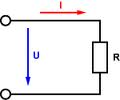
\includegraphics{images/ohmsche.jpeg}
		}
		\caption{Schaltplan einer einfachen U-I-Messung}
	\end{figure}
	
	Das Ohmsche Gesetz liefert hierfür:
	\begin{gather*}
	U=R\cdot I
	\end{gather*}
	Gesucht ist der zugehörige Widerstand $R$.\\
	
	\begin{figure}
		\parbox{\linewidth}{
			\centering
			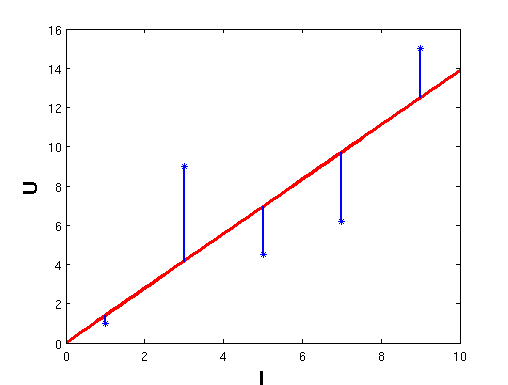
\includegraphics[width=0.5\linewidth]{images/linausgl2.png}
		}
		\caption{Linearausgleich einer U-I-Messung mit Ursprungsgerade als Modellfunktion}
	\end{figure}
	
	Wird jetzt davon ausgegangen dass die $I_i$ exakt sind, wird das $R$ gesucht, 
	für das $RI_i$ im Mitttel den minimalen Abstand zu $U_i$ hat.
	Genauer gesagt berechne
	\begin{gather*}
	\min_{r\in\R} \sum_{i=1}^{m}(U_i-rI_i)^2
	\end{gather*}
	\textbf{Vorsicht: } Es wird \textbf{nicht} die Gerade (bzw. der lineare Untervektorraum) mit 
	minimalem euklidischem Abstand zu $(I_i,U_i)$ gesucht! \\
	Dieses Problem ist nichtlinear und aufwendig zu lösen.
\end{Bspe}


\subsectione{Lineares Ausgleichsproblem} \index{Ausgleichsproblem!linear}
Gegeben seien Messdaten $(t_i, b_i)$ mit $t_i, b_i\in \R$ für $i=1, \dots, m$ 
und die Abhängigkeit $b(t)$ werde beschrieben durch eine Modellfunktion,
welche linear von den unbekannten Parametern $x_1, \cdots, x_n$ des Modells abhängt,
d.h.
\begin{gather*}
b(t) = a_1(t)x_1 + \dots + a_n(t) x_n
\end{gather*}
Für exakte Messdaten $b_i$ würde 
\begin{gather*}
b(t_i) = b_i \quad \forall i\in\{1,\cdots , m\}
\end{gather*}
gelten.\\
Im Allgemeinen werden jedoch $m\geq n $ Messwerte $b_i$ bestimmt,
und hiermit die $n$ Parameter $x_i$ so gewählt, dass die kleinsten
\textbf{Fehlerquadrate auftreten}:
\begin{gather}
\min_{x_1, \dots x_n} \sum_{i=1}^{m} (b_i-b(t_i))^2 \label{IV.3.1}
\end{gather}
(Nach Gauß kann \eqref{IV.3.1} auch aus der Maximum-Likelihood-Methode\index{Maximum-Likelihood-Methode}
für einen stochastischen Ansatz hergeleitet werden.)\\

Definiere:
\begin{align*}
b &= (b_i)_{i=1,\dots, m}\in \R^m \\
x &= (x_j)_{j=1,\dots, n}\in \R^n \\
A &= (a_j(t_i)) _{\substack{i=1,\dots, m \\ j= 1, \dots, n}} \in \R^{m\times n}
\end{align*}
Damit ist \eqref{IV.3.1} äquivalent zum \textbf{linearen Ausgleichsproblem}:\\
Zu gegebenem $b\in\R^m$ und $A\in\R^{m\times n}$ mit $m\geq n$
ist das $\overline{x} \in \R^n$ gesucht mit 
\begin{gather}
\nn{b-A\overline{x}}_2 = \min_{x\in\R^n} \nn{b-Ax}_2
\label{IV.3.2}
\end{gather}
Das entspricht der \enquote{Lösung} eines überbestimmten, i.A. nicht erfüllbaren
GLS $Ax=b$.\\
Aufgrund der $l_2$-Norm ist $\overline{x}$ gegeben durch die 
orthogonale Projektion von $b$ auf den Bildraum $R(A) $ \index{Bildraum}, wie gleich gezeigt wird. \\

\begin{tikzpicture}[rotate=0,line cap=round,line join=round,>=triangle 45,x=1.0cm,y=1.0cm]
% Draw region settings
\clip(1.8,-3.2) rectangle (13.5,3);
% Right angle
\draw [shift={(8,0)}] (90:0.6) arc (90:180:0.6);
\fill (7.75,0.25) circle (1pt);
% Plane
\draw (2,2)-- (10,2)-- (13,-2)-- (5,-2)-- cycle;
\draw[<-] (9,1)-- (12,2) node [anchor=west] {$R(A)$};		
% vectors
\draw[->] (6,0) node[anchor=north east] {0} -- (8,0) node[anchor=north west] {$A\overline{x}$};
\draw[->] (6,0)--(8,2.46) node[anchor=south west] {$b$};
\draw[dashed] (8,0)-- (8,2.46);
\fill  (6,0) circle (2pt);
\fill  (8,0) circle (2pt);	
\fill  (8,2.46) circle (2pt);
\end{tikzpicture}

% \subsectione{Projektionssatz} 
\begin{Satze}[Projektionssatz]
	\index{Projektionssatz} \label{4.3.3}
	Sei $V$ ein reeller Vektorraum mit einem Skalarprodukt $\scp{\cdot}{\cdot}$
	und der induzierten Norm $\nn{v}\coloneqq \sqrt{\scp{v}{v}}$.
	Sei $U\subset V$ ein endlich dimensionaler Untervektorraum und sei
	\begin{gather*}
	U^\bot \coloneqq \left\{ v\in V  \, \middle\vert \, \scp{v}{u} = 0 ~~ \forall u\in U \right\}
	\end{gather*}
	Dann gilt:
	\begin{enumerate}[1)]
		\item Zu jedem $v\in V$ existiert genau ein $\overline{u}\in U$, 
		so dass $v-\overline{u}\in U^\bot$, d.h.
		\begin{gather*}
		\scp{v-\overline{u}}{u} = 0 \quad \forall u \in U
		\end{gather*}
		Dies definiert die \textbf{orthogonale Projektion} \index{orthogonale Projektion}
		\begin{gather*}
		P:V\rightarrow U, \quad v\mapsto \overline{u}= Pv
		\end{gather*}
		\item Zu jedem $v\in V $ bestimmt $P\cdot v$ die eindeutige Lösung
		\begin{gather*}
		\nn{v-Pv}= \min_{u\in U} \nn{v-u}
		\end{gather*}
		Also gilt mit einem eindeutigen $\overline{u}= Pv$, dass 
		\begin{gather}
		\nn{v-\overline{u}} = \min_{u\in U} \nn{v-u} 
		\Longleftrightarrow \scp{v-\overline{u}}{u} = 0 \quad \forall u\in U
		\label{IV.3.3}
		\end{gather}
	\end{enumerate} 	
\end{Satze}

\begin{proof}
	\begin{enumerate}[1)]
		\item Sei $\{u_1, \dots , u_n \}$ eine Orthonormalbasis von $U$ 
		und $\overline{u}\in U $. \\
		Daraus folgt:
		\begin{gather*}
		\exists ! \, (\alpha_i)_{i=1,\dotsc,n} \subset \R: \overline{u} = \sum_{i=1}^{n} \alpha_i u_i
		\end{gather*}
		Damit gilt:
		\begin{alignat*}{3}
		&&0 &= \scp{v-\overline{u}}{u} &\quad& \forall u \in U \\
		&\Longleftrightarrow \quad& 0 &= \scp{v- \sum_{i=1}^{n} \alpha_i u_i}{u_i} &\quad &\forall j=1, \dots , n\\
		&\Longleftrightarrow  & \scp{v}{u_j} &= \sum_{i=1}^{n} \alpha_i \scp{u_i}{u_j} = \alpha_j
		\end{alignat*}
		Setze also 
		\begin{align}
		\nonumber
		P\cdot v &= \overline{u} \\
		& = \sum_{i=1}^{n} \scp{v}{u_i} u_i \in U
		\label{IV.3.4}
		\end{align}
		dann ist $\overline{u}$ die eindeutig bestimmte Lösung für $ v-\overline{u} \in U^\bot$
		
		IMAGE~MISSING \\
		
		Sei  $u\in U$. Dann gilt:
		\begin{align}
		\nonumber
		\nn{v-u}^2 &= \nn{v-\overline{u}+\overline{u} -u}^2 \\ \nonumber
		&= \nn{v-\overline{u}}^2 +
		\underbrace{\scp{v-\overline{u}}{\overbrace{\overline{u}-u}^{~~\in U}}}_{=0}
		+ \nn{u-\overline{u}}^2 \\
		&= \nn{v-\overline{u}}^2 + \nn{u-\overline{u}}^2
		\label{IV.3.5}
		\end{align}
		(Dies ist anschaulich der Satz des Pythagoras.)
	\end{enumerate}
\end{proof}


% \subsectione{Satz}
\begin{Satze}
	Der Vektor $\overline{x} \in\R^n$ ist genau dann Lösung des linearen Ausgleichsproblems
	\begin{gather*}
	\min_{x\in\Ren} \nn{b-Ax}_2 \, ,
	\end{gather*}
	falls er die Normalengleichung
	\begin{gather}
	A^TA\overline{x} = A^Tb
	\label{IV.3.6}
	\end{gather}
	erfüllt. \\
	Insbesondere ist $\overline{x}$ eindeutig,
	falls $A\in \R^{m\times n}$ maximalen Rang $n\leq m$ hat.
\end{Satze}

\begin{proof} Bezeichne
	$V= \R^m, U= R(A) = \left\{Ax \, \middle|  \, x \in\Ren \right\}, b \in \R^m$.\\
	Nach \eqref{IV.3.3} gilt:
	\begin{alignat*}{2}
	&&\nn{b-A\overline{x}}_2 &= \min_{x\in\Ren} \nn{b-Ax}_2 \\
	&\Leftrightarrow \quad & \scp{b-A \overline{x}}{Ax} &= 0 \quad \forall x\in \Ren \\
	&\Leftrightarrow & \scp{A^T(b-A\overline{x})}{x} &= 0 \quad  \forall x\in\Ren \\
	&\Leftrightarrow & A^T(b-A\overline{x}) &= 0 \\
	&\Leftrightarrow & A^TA\overline{x} &= A^Tb
	\end{alignat*}
	Nach dem Projektionssatz \ref{4.3.3} existiert mindestens ein eindeutiges
	$\overline{y} = P b$.
	Für dieses $\overline{y}$ ist $\overline{x}\in \Ren $ mit $\overline{y} = A\overline{x}$
	eindeutig bestimmt, falls $A$ injektiv ist, d.h. falls $rang(A) = n$. 
\end{proof}

Ähnlich zum Skalarprodukt ist die relative Kondition von $(P,b) $ schlecht, 
falls $b$ fast senkrecht zu $U$ steht.
Die relative Kondition des linearen Ausgleichsproblems hängt zusätzlich von $cond(A)$ ab.


\subsectione{Lösung der Normalgleichung}
Falls $rang(A) = n$, ist $A^TA$ spd und das Cholesky-Verfahren ist anwendbar. \\
Dafür ist
\begin{enumerate}[1.]
	\item $A^TA$ zu berechnen:
	\begin{description}
		\item[Aufwand] ca. $\frac{1}{2}n^2m$ Multiplikationen 
		\item[Kondition] häufig schlecht, da $\frac{1}{2}n^2$ Skalarprodukte berechnet werden
	\end{description}
	\item die Cholesky-Zerlegung von $A^TA $ durchzuführen:
	\begin{description}
		\item[Aufwand] ca. $\frac{1}{6}n^3$ Multiplikationen 
		\item[Kondition] Für $A\in\R^{m\times n}$ mit $m\geq n$ und $rang(A)=n$ gilt:
		\begin{gather}
		cond_2(A^TA) = cond_2(A)^2 \label{IV.3.7}
		\end{gather}
		(siehe Übungsaufgabe 19)
	\end{description}
\end{enumerate}
Also überwiegt für $m\gg n$ der Aufwand $A^tA$ zu berechnen.
Die auftretenden Konditionen entsprechen i.d.R. nicht dem des Ausgangsproblems.\\
Damit ist die 
\textbf{Cholesky-Zerlegung \index{Cholesky-Zerlegung} für Normalgleichungen ungeeignet}.


% \subsectione{Satz}
\begin{Satze}
	Sei $A\in \R^{m\times n} $ mit $m\geq n$ und $rang(A) = n$,
	sei $b\in\R^m$ und besitze $A$ eine Zerlegung
	\begin{gather*}
	A= Q\begin{pmatrix}R\\0\end{pmatrix}
	\end{gather*}
	mit einer orthogonalen Matrix $Q\in R^{m\times m}$ und 
	einer oberen Dreiecksmatrix $R\in \R^{n\times n}$. \\
	Dann ist $R$ invertierbar. \\
	Bezeichne 
	\begin{gather}
	\begin{pmatrix} \overline{b}_1 \\ \overline{b}_2\end{pmatrix}
	\coloneqq Q^T\cdot b
	\label{IV.3.9}
	\end{gather}
	dann ist
	\begin{gather}
	\overline{x} = R^{-1} \overline{b}_1 
	\label{IV.3.10}
	\end{gather}
	die Lösung des linearen Ausgleichsproblems und
	\begin{align*}
	\nn{\overline{b}_2} &= \nn{b-A\overline{x}} \\
	& = \min_{x\in \Ren }\nn{b-Ax}
	\end{align*}
\end{Satze}

Zur Erinnerung:
\begin{align*}
Q \text{ orthogonal} &:\Leftrightarrow QQ^T = I \\
&\, \Leftrightarrow Q^{-1} = Q^T
\end{align*}
Weiterhin ist $Q$ längenerhaltend\index{längenerhaltend}, d.h. $\nn{Qv}_2 = \nn{v}_2$ 
und somit folgt
\begin{gather}
\nonumber
\nn{Q}_2 = \nn{Q^{-1}}_2 = 1 \quad \text{und} \\
cond_2(Q) = 1
\label{IV.3.11}
\end{gather}

\begin{proof} $R$ ist invertierbar, da 
	\begin{align*}
	rang(R) &= rang(Q^{-1}\cdot A) \\	
	& = rang(A) \\
	&= n
	\end{align*}
	Außerdem gilt:
	\begin{align*}
	\nn{b-Ax}_2^2 & = \nn{Q(Q^Tb-\begin{pmatrix}R\\0\end{pmatrix}x)}_2^2 \\
	&=  \nn{Q^Tb-\begin{pmatrix}Rx\\0\end{pmatrix}}_2^2  \\
	&\overset{\mathllap{\text{$Q$ längenerhaltend}}}{=}
	\nn{\overline{b}_1 - Rx}_2^2  + \nn{\overline{b}_2^2}
	\end{align*}
	wird minimal für $R\overline{x} = \overline{b}_1$
\end{proof}

Da $Q$ längenerhaltend ist, folgt mit \ref{3.2.13} b)
($cond_A \coloneqq \frac{\max \nn{Ax}}{\min \nn{Ax}}$)
sofort:
\begin{gather*}
cond_2(A) = cond_2(R)
\end{gather*}
Die auftretende Kondition entspricht also der des Ausgleichsproblems.


% \subsectione{Bemerkung}
\begin{Beme}
	Sei $A\in \Renn$ invertierbar und habe ein QR-Zerlegung, d.h. es existiert
	eine orthogonale Matrix $Q$ und eine obere Dreiecksmatrix $R$, so dass:
	\begin{gather*}
	A= Q\cdot R
	\end{gather*}
	Dann kann das Gleichungssystem $Ax=b$ wie folgt gelöst werden:
	\begin{enumerate}[1.]
		\item Setze $z=Q^Tb$, was Kondition 1 hat.
		\item Löse durch Rückwärtssubstitution $Rx=z$.
	\end{enumerate}
\end{Beme}


%-------------------------------------------------------------

\sectione{Orthogonalisierungsverfahren}\index{Orthogonalisierung}
\marginpar{12.11.2014}
Konsturiere eine QR-Zerlegung
\begin{gather}
A= Q\cdot \begin{pmatrix} R\\0 \end{pmatrix}
\label{IV.4.1}
\end{gather}
durch einen Eliminationsprozess:
\begin{gather}
A \rightarrow Q^{(1)}A \rightarrow Q^{(2)} Q^{(1)}A \rightarrow Q^{(p)}\cdot \dotsc \cdot Q^{(1)}A
= \begin{pmatrix} R\\0 \end{pmatrix}\, .
\label{IV.4.2}
\end{gather}
mit orthogonalen Matrizen $Q^{(i)}$.
Dann gilt
\begin{gather}
Q= Q^{(1)T}\cdot \dotsc \cdots {Q^{(p)T}}
\label{IV.4.3}
\end{gather}
Dies ist im Gegensatz zur $LR$-Zerlegung aufgrund von $cond(Q^{(i)})= 1$ immer stabil.\\

Für $Q\in\R^{2\times 2}$ gibt es zwei mögliche Anschauungen, nämlich:
\begin{enumerate}[a)]
	\item Drehung ~~~ IMAGE~MISSING
	\item Spiegelung ~~~ IMAGE~MISSING
\end{enumerate}

\extrasection{a)}{Givens-Rotation}
Es wird eine Drehung auf den 1. Einheitsvektor durchgeführt:\\

IMAGE~MISSING\\

\begin{gather*}
a=\begin{pmatrix}a_1 \\ a_2\end{pmatrix} \rightarrow \begin{pmatrix}\alpha \\ 0 \end{pmatrix}
= \alpha e_1
\end{gather*}
d.h. Elimination von $a_2$ mit
\begin{gather*}
\nn{\alpha e_1}_2 = \nn{a}_2
\end{gather*}
Also gilt für $\alpha$
\begin{gather*}
\alpha=\pm \nn{a}_2
\end{gather*}
Drehuungen werden beschrieben durch
\begin{gather*}
Q = \begin{pmatrix}
cos(\theta) & sin(\theta)\\
-sin(\theta) & cos(\theta)
\end{pmatrix}
\eqqcolon \begin{pmatrix}
c & s\\
-s & c
\end{pmatrix}\qquad \theta \in[0,2\pi)
\end{gather*}
und es muss gelten
\begin{gather*}
Qa = \begin{pmatrix}\alpha \\ 0 \end{pmatrix}
\end{gather*}
Hiermit folgt für $\nn{a}= 0$
\begin{align}
\nonumber
c&=1, s=0\\ \nonumber
c&=\frac{a_1}{\alpha},  s= \frac{a_2}{\alpha}\quad \text{mit}\\
\alpha & = \pm \sqrt{a_1^2+a_2^2}
\label{IV.4.4}
\end{align}
für $\nn{a}\neq 0$.\\
Im Folgenden wird dies kurz mit
\begin{gather*}
[c,s] = givens(a_1, a_2)
\end{gather*}
bezeichnet. \\
Als \textbf{Givens-Rotation}\index{Givens-Rotation} wird eine Matrix der Form
\begin{gather}
\Omega _{k,l} = \begin{pmatrix}
1 &&&&&&&&& \\
& \ddots\\
&& 1\\
&&& \mathbf{c} &&&& \mathbf{s} \\
&&&& 1\\
&&&&& \ddots \\
&&&&&& 1\\
&&& -\mathbf{s} &&&& \mathbf{c} \\
&&&&&&&& \ddots \\
&&&&&&&&& 1\\
\end{pmatrix}
\begin{array}{l}
\\   \leftarrow \text{$k$-te Zeile}
\\ \\ \\ \\ \leftarrow \text{$l$-te Zeile}
\end{array}
\label{IV.4.5}
\end{gather}
mit $c^2+s^2=1$ und $k<l$ bezeichnet.\\
Es folgt:
\begin{align*}
\Omega_{kl} A &= \widetilde{A} \quad \text{mit} \\
\widetilde{a}_{ij}  &= a_{ij} \quad \text{ für } i\neq k,l \\
\widetilde{a}_{kj} & = ca_{kj}+sa_{lj} \\
\widetilde{a}_{lj} & = -sa_{kj} + ca_{lj}
\end{align*}
Demnach werden nur die $k$-te und $l$-te Zeile werden verändert. \\
Falls nun $[c,s] = givens(x_k, x_l)$ gilt
\begin{gather}
\Omega_{k,l}\cdot x = \begin{pmatrix}
x_1 \\ \vdots \\x_{k-1} \\\alpha \\ x_{k+1}
\\\vdots \\
x_{l-1} \\ 0 \\x_{l+1} \\\vdots \\x_n
\end{pmatrix}
\qquad
\quad \text{mit~~}
\alpha = \pm \nn{  \begin{pmatrix} x_k \\ x_l\end{pmatrix}}_2
\label{IV.4.6}
\end{gather}
d.h. eine Givens-Rotation erzeugt eine Null.\\
Da nun
\begin{gather*}
\R^{m\times n}\ni \begin{pmatrix}
* & * &* & \dots   \\
0 & * &     \\
0 & 0 & \ddots \\
\vdots \\
0 & 0 & 0 & \dots & *		
\end{pmatrix}
= \begin{pmatrix} R\\0\end{pmatrix}
\end{gather*}
gilt, sind
\begin{gather*}
p=\sum_{j=1}^{n}(m-j)
\end{gather*}
Givens-Rotationen nötig, um eine QR-Zerlegung nach \eqref{IV.4.1} zu erzeugen.
Und eine Rotation, welche $a_{ij} $ auf 0 setzt, ist durch zugehörige 
$(c_{ij}, s_{ij}) $ gegeben.\\

Für eine 3x4-Matrix sieht das Verfahren folgendermaßen aus:

\begin{align*}
A= &
\left(\begin{array}{lccc}
*~ &&&\\
* &&* \\
* \rcurvearrownw \\ * \lcurvearrowsw
\end{array}\right)
\quad \overset{\Omega_{3,4}}{\longrightarrow} \quad
\left(\begin{array}{lccc}
*~ &&&\\
* \rcurvearrownw && *\\
* \lcurvearrowsw \\
0
\end{array}\right)
\quad \overset{\Omega_{1,2}}{\longrightarrow} \quad
\left(\begin{array}{lccc}
* \rcurvearrownw\\
* \lcurvearrowsw && *& \\
0 \\
0
\end{array}\right)\\
\quad \overset{\Omega_{2,3}}{\longrightarrow} \quad
&\left(\begin{array}{lccc}
*~~ \\
0 && *&~ \\
0 \\
0
\end{array}\right)
\quad \overset{\Omega_{3,4}}{\longrightarrow} \quad	
\left(\begin{array}{clcc}
* & *\\
0 & *  \rcurvearrownw  & *& \\
0 & * \lcurvearrowsw \\
0 & 0
\end{array}\right)
\quad \overset{\Omega_{2,3}}{\longrightarrow} \quad	
\left(\begin{array}{cccl}
* & *  & * \\
0 & *  & * \\ 
0 & 0 & * \rcurvearrownw\\
0 & 0 & *  \lcurvearrowsw 
\end{array}\right) \\
\quad \overset{\Omega_{3,4}}{\longrightarrow} \quad	
& \left(\begin{array}{cccc}
* & *  & *  \\
0 & *  & * \\ 
0 & 0 & * \\
0 & 0 & 0
\end{array}\right)
= \begin{pmatrix}
R \\ 0 
\end{pmatrix}
\end{align*}


Es ergibt sich:

\subsectione{Givens-QR-Algorithmus} \index{Givens-QR-Algorithmus}

\begin{pseudocode}{0.7\linewidth}
	\textbf{for} $j=1, \dotsc , n$ \\
	|~	\>	\textbf{for} $i=m, m-1, \dotsc , j+1$ \\
	|~	\>		|~	\>\% \textit{setze $a_{ij}$ auf 0} \\
	|~	\>		|~	\>$[c,s] = givens(a_{i-1,j}, \dotsc, a_{ij}) $\\
	|~	\>		|~	\>speichere $c$ und $s$ für $a_{ij}$ \\
	|~	\>		|~	\>$A(i-1:j, j:h) =\left( \begin{smallmatrix}c & s\\ -s & c	\end{smallmatrix}\right) * A(i-1:j, j:n)$ \\
	|~	\> \textbf{end}\\
	\textbf{end}							
\end{pseudocode}

% \subsectione{Bemerkungen} 
\begin{Beme}~
	\begin{enumerate}[a)]
		\item $A(i-1 : i, 1 : j-1) = 0$ und ist daher nicht zu berechnen oder
		zu speichern. Der Speicherplatz kann für die Speicherung der
		Givensrotationen benutzt werden.
		\item  $R$ steht anschließend in $A$.
		\item Die Bestimmung der Länge $|\alpha|$ wird so ausgeführt, dass over- ¨
		oder underflow vermieden wird. Weiterhin wird das Vorzeichen
		von $c$ oder $s$ festgelegt, so dass aufgrund von $c^2+s^2=1$ nur
		ein Wert $\rho$ gespeichert werden muss. Hiermit wird auch das
		Vorzeichen von $\alpha$ festgelegt:\\
		\begin{description}
			\item[$a_2=0$:] Setze $c=1, s=0, \alpha = a_1$, merke $\rho=1$.
			\item[$|a_2|>|a_1|$:] Setze $\tau= \frac{a_1}{a_2}, s=\frac{1}{\sqrt{1+\tau^2}}, c=s\cdot\tau, \alpha =a_2\sqrt{1+\tau^2}$, merke $\rho=\frac{c}{2}$.
			\item[$|a_1|\geq|a_2|$:] Setze $\tau= \frac{a_2}{a_1}, c=\frac{1}{\sqrt{1+\tau^2}}, s=c\cdot\tau, \alpha =a_1\sqrt{1+\tau^2}$, merke $\rho=\frac{2}{s}$.
		\end{description}
		\item Aufgrund von c) muss nur $\rho$ gespeichert werden:
		\begin{description}
			\item[$\rho=1$:] Setze $c=1, s=0$.
			\item[$|\rho|<1$:] Setze $c=2\rho , s= \sqrt{1-c^2}$.
			\item[$|\rho|>1$:] Setze $s=\frac{2}{\rho}, c=\sqrt{1-s^2}$.
		\end{description}
	\end{enumerate}
	Hiermit können alle notwendigen Givens-Rotationen als untere
	Dreiecksmatrix zusammen mit $R$ in $A$ gespeichert werden.
\end{Beme}



\subsectione{Aufand des Givens-QR-Algorithmus}
\begin{enumerate}[a)]
	\item $m\approx n$\\ $\rightarrow $  ca. $\frac{4}{3}n^3$ Multiplikationen
	und $\frac{1}{2}n^2$ Quadratwurzeln nötig \\
	Die Givens-QR-Zerlegung ist somit ungefähr viermal so aufwändig
	wie die Gauß-Elimination, dafür jedoch stabil.
	\item $m\gg n$\\ $\rightarrow $ ca. $2n^2m$ Multiplikationen und 
	$mn$ Quadratwurzeln nötig \\
	Das Verfahren ist daher zwei- bis viermal so aufwändig wie das
	Cholesky-Verfahren für die Normalgleichungen, aber stabil.
	\item Bei Hessenberg-Matrizen, d.h. Matrizen mit der Gestalt
	\begin{gather}
	A= \begin{pmatrix}
	* & \dots&& * \\
	*&* \\
	&\ddots& \ddots \\
	\\
	0 &&& * 
	\end{pmatrix}
	\label{IV.4.7} \, ,
	\end{gather}
	also $a_{ik} = 0 \forall i<k+1$,
	sind nur $(n-1)$ Givens-Rotationen auszuführen. \\
	Diese Matrizen tauchen z.B. bei Eigenwertberechungen auf
	und sind dort ein wichtiger Bestandteil der Verfahren.
\end{enumerate}


\extrasection{b)}{Householder-Reflexion}

Es sei $H$ eine Hyperebene im $\R^m$ und zusätzlich ein Vektor $a\in\R^m$ gegeben. \\

IMAGE~MISSING \\

Gesucht ist nun die Reflexion $Q$, so dass
\begin{gather*}
Qa = \alpha e_1 = \begin{pmatrix} \alpha \\ 0\\\vdots\\0\end{pmatrix}
\qquad \text{mit } \alpha = \pm \nn{a}
\end{gather*}
Mit \begin{gather}
v=a-\alpha e_1 
\label{IV.4.8}
\end{gather}
gegeben, welches senkrecht zu $H$ steht.\\
Damit Stellenauslöschungen in $v$, d.h. in $v_1$, vermieden werden,
wähle ein entsprechendes Vorzeichen für $\alpha$, also 
\begin{gather}
\alpha = -sign(a_1)\nn{a}_2 
\label{IV.4.9}
\end{gather}
Die zugehörige Reflexion $Q$ ist  gegeben durch \\
\begin{center}
	\begin{tikzpicture}[line cap=round,line join=round,>=triangle 45,x=1.0cm,y=1.0cm]
	\clip(0.7,1) rectangle (6,5);
	\draw [shift={(4.32,3.49)}] (0,0) -- (36.87:0.6) arc 	(36.87:126.87:0.6) -- cycle;
	\draw [shift={(1.53,2.76)}] (0,0) -- (-53.13:0.6) arc (-53.13:36.87:0.6) -- cycle;
	\draw [domain=0.7:6] plot(\x,{(--1--3*\x)/4});
	\draw (5.26,4.38) node[anchor=north west] {$$H$$};
	\draw [->] (2.18,1.89) -- (0.84,3.68);
	\draw [->] (2.18,1.89) -- (3.66,4.36);
	\draw [->] (2.18,1.89) -- node[anchor=north east] {$w$} (1.53,2.76);
	\draw [->,dash pattern=on 2pt off 2pt] (2.18,1.89) -- node[anchor=north] {$Qx$} (4.97,2.61);
	\draw [->] (3.66,4.36) -- (4.97,2.61);
	\fill(4.37,3.84) circle (0.02);
	\draw [dash pattern=on 2pt off 2pt] (1.53,2.76)-- (3.66,4.36);
	\fill(1.88,2.71) circle (0.02);
	
	\draw (1.26,3.46) node {$v$};
	\draw (4.3,3.1) node {$2w$};
	\end{tikzpicture}
\end{center}		

wobei
\begin{align}
\nonumber
w &= \scp{\frac{v}{\nn{v}}}{x} \cdot \frac{v}{\nn{v}} \\ %\nonumber
Qx &= x-2w = x-2\frac{v^Tx}{v^Tv}v 
= (I-2\frac{vv^T}{v^Tv})x 
\label{IV.4.10}\\
Q  &= I-2\frac{vv^T}{v^Tv}&& vv^T \in \Renn,\,\, v^Tv\in\R
\label{IV.4.11}
\end{align}
und heißt \textbf{Householder Reflexion} \index{Householder Reflexion}
(wurde  1958 von Householder eingeführt).  \\
Für die spezielle Wahl \eqref{IV.4.8} mit \eqref{IV.4.9} vom Vektor $v$ folgt
\begin{align}\nonumber
vv^T = \nn{v}^2 &= \nn{a}^2 - 2\alpha\scp{a}{e_1} + \alpha^2 \\ \nonumber
&= -2\alpha(a_1-\alpha) \\
& = -2\alpha v
\label{IV.4.12}
\end{align}


% \subsectione{Bemerkung}
\begin{Beme}
	\label{4.4.4}~
	\begin{enumerate}[a)]
		\item Q ist symmetrisch
		\item Q ist orthogonal
		\item Q ist involutorisch, d.h. $Q^2 = I$ ~~(bzw. gilt $Q^{-1}= Q^T=Q$)
	\end{enumerate}
	Die Householder Reflexion setzt nicht nur eine Null,
	sondern im Vektor gleich alle gewünschten Nullen
	\begin{align*}
	\text{\textbf{Rotation: }}&
	\quad \begin{pmatrix} * \\ * \\ *	\end{pmatrix}
	\rightarrow \begin{pmatrix} * \\ * \\0	\end{pmatrix}
	\rightarrow \begin{pmatrix} * \\0\\0	\end{pmatrix} \\
	\text{\textbf{Reflexion: }}&
	\quad \begin{pmatrix} * \\ * \\ *	\end{pmatrix}
	\rightarrow \begin{pmatrix} *\\0\\0	\end{pmatrix}
	\end{align*}
	Um die erste Spalte in $A$ auf die gewünschte Gestalt zu bringen,
	bestimme $Q^{(1)}$ wie oben, indem die erste Spalte als $a$ gewählt wird:
	\begin{gather*}
	A\rightarrow A^{(1)} = Q^{(1)} A =
	\begin{pmatrix}
	\alpha^{(1)} \\
	0 &*&~~\\
	\vdots \\
	0
	\end{pmatrix}
	\end{gather*}
	In der $k$-ten Spalte sollen nun die $(k-1)$-ten Zeilen und die $(k-1)$-ten Spalten
	bleiben und die Restmatrix verändert werden.\\
	
	\begin{align*}
	A^{(k-1)} &=
	\begin{pmatrix}
	*  &&&&&\\
	&\ddots &&&& * \\
	&&*&&\_&\_&\_ \\
	&&0&|&\\
	&0&\vdots&| &&T^{(k-1)}\\
	&&\vdots&  |\\
	&&0&  |
	\end{pmatrix}
	\begin{array}{l}
	\\
	\shortleftarrow (k-1) \text{-te Zeile} \\
	\\\\\\\\
	\end{array}\\
	&\phantom{= \, (} \begin{array}{ccl}
	~&~&~ \uparrow (k-1)\text{-te Spalte}
	\end{array}
	\end{align*}
	
	Setze also
	\begin{gather}
	Q^{(k)} = \begin{pmatrix}
	I_{k-1} & 0 \\
	0 & \overline{Q}^{(k)} \, ,
	\label{IV.4.13}
	\end{pmatrix}
	\end{gather}
	wobei $\overline{Q}^{(k)} $ durch die erste Spalte von $T^{(k)}$, d.h.
	\begin{gather}
	a= (a_{i,k}^{k-1})_{i=k,\dotsc, m} \subset \R^{m+1-k}
	\label{IV.4.14}
	\end{gather}
	bestimmt wird. Dann gilt
	\begin{gather*}
	Q^{(k)}A^{(k-1)} =
	\begin{pmatrix}
	*  &&&&&\\
	&\ddots &&&& * \\
	&&*&&\_&\_&\_&\_ \\
	&&0&|&* \\
	&0&\vdots&|&0&* \\
	&&\vdots&  |&\vdots &&\ddots\\
	&&0&  |&0&&&*
	\end{pmatrix}
	\end{gather*}
	Nach insgesamt 
	\begin{gather}
	p=\min (m-1, n)
	\label{IV.4.15}
	\end{gather}
	Schritten erhalten wir für $A\in \R^{m\times n}$
	\begin{gather}
	Q^TA = Q^{(p)}\cdot \dotsc \cdot Q^{(1)}A 
	= \begin{pmatrix} R\\0\end{pmatrix}\, ,
	\end{gather}
	wobei Bemerkung \ref{4.4.4} auch für 
	$Q^T= Q^{(p)}\cdot \dotsc \cdot Q^{(1)} $ und somit auch für
	\begin{gather}
	Q = Q^{(1)}\cdot \dotsc \cdot Q^{(p)}
	\label{IV.4.16}
	\end{gather}
	gilt.
\end{Beme}



%----------------------------------------------------------------

\subsectione{Speicherung}
\marginpar{17.11.2014}
Gespeichert werden müssen die obere Dreiecksmatrix $R$ und die 
\textbf{Householdervektoren} \index{Householdervektoren}
$v^{(i)}\in \R{m+1-i}$.
Die Diagonalelemente von $R$ sind $r_{ii} = \alpha^{(i)}$. \\
Folgende Speicheraufteilung ist möglich:
\begin{gather*}
A \longrightarrow \left(
\begin{array}{rrrrr}
|&&& R \\
|&| \\
v^{(1)}| & v^{(2)}|&\ddots ~~\\
| &|&\phantom{v^{(i)}}|& v^{(p)}			
\end{array}
\right)
\quad \text{und} \quad 
\begin{pmatrix}
\alpha^{(1)} \\ \vdots \\ \\ \alpha^{(p)}
\end{pmatrix}
\end{gather*}

Wohlgemerkt kann so auch $A\in \R{m\times n}$ mit $m<n$ bearbeitet werden,
dann wird $A$ zu:

\imagemissing{Zerlegung einer mxn-Matrix für $m<n$}

Falls zusätzlich $v^{(i)}$ so normiert ist,
dass $v_1^{(i)} = 1$ ist, braucht diese Komponente nicht gespeichert werden 
und $R$ kann komplett in $A$ gespeichert werden.



\subsectione{Householder QR-Algorithmus}
\begin{pseudocode}{\linewidth}
	\textbf{for} $j = 1,\dots, \min(m - 1, n)$ \\
	|	\>	// berechne $\alpha$ für $a = A(j : m, j)$ \\
	|	\>	$\alpha(j) = -sign(A(j, j))\sqrt{A(j:m, j)^T A(j:m, j)}$ \>\>\>\> siehe \eqref{IV.4.9}\\
	|	\>  // berechne $A(j:m,j)=v=a-\alpha e_1$ \\
	|	\>	$A(j,j)=A(j,j)-\alpha(j)$ \>\>\>\> siehe \eqref{IV.4.8}\\
	|	\> // berechne $-\scp{v}{v} = \alpha(a_1 - \alpha) = \alpha v_1$ \\
	|	\> $\beta = \alpha(j)A(j, j)$\>\>\>\> siehe \eqref{IV.4.12}\\
	|	\> // berechne $\overline{Q}^{(j)}T^{(j)}$ 
			aber nicht mehr die erste Spalte, welche $\alpha(j)e_1$ ist\\
	|	\> \textbf{for} $l = j + 1 : n$\\
	|		\>\> // setze $v_x = -2{(v^Tx)}{(v^Tv)}^{-1}$\\
	|		\>\> $v_x = A(j : m, j)^TA(j:m,l)\cdot \frac{1}{\beta}$ \>\>\>siehe \eqref{IV.4.10}\\
	|		\>\> // berechne  $\overline{Q}^{(j)}x=x+v_x\cdot v$\\
	|		\>\> $A(j:m,l) = A(j:m,l)+v_xA(j:m,l)$ \>\>\> siehe \eqref{IV.4.10}\\
	|	\>\textbf{end}\\
	\textbf{end}
\end{pseudocode}


\subsectione{Berechnung von $Q^Tb$}
Zur Lösung eines Gleichungssystems oder eines linearen Ausgleichsproblems
muss noch $Q^Tb=Q^{(p)}\cdot \dots \cdot Q^{(1)}$ berechnet werden.

\begin{pseudocode}{0.7\linewidth}
	\textbf{for} $j=1,\dots, \min\{m-1,n\}$\\
	|	\> // beachte \eqref{IV.4.13}, also $b(1:j-1)$ bleibt gleich\\
	|	\> // setze $v_x=-2(v^Tb)(v^Tv)^{-1}$\\
	|	\> $v_x=\big(A(j:m,j)^Tb(j:m)\big)\cdot \big(\alpha(j)A(j,j)\big)^{-1}$ \\
	|	\> // berechne $\overline{Q}^{(j)} b=b+v_xv$\\
	|	\> $b(j:m) = b(j:m)+v_xA(j:m,j)$\\
	\textbf{end}
\end{pseudocode}


\subsectione{Aufwand für den Householder-QR-Algorithmus}
\begin{enumerate}[a)]
	\item Falls $m\approx n$ sind ungefähr $\frac{2}{3}n^3$ Multiplikationen notwendig
	und ist somit ungefähr doppelt so teuer wie die LR-Zerlegung, ist aber stabil.
	\item Falls $m\gg n$ sind ungefähr $2mn^2$ Multiplikationen notwendig.
	Der Aufwand ist daher ungefähr so hoch wie beim Cholesky-Verfahren für Normalgleichungen,
	aber stabil.
\end{enumerate}


% Kap. 5: Numerische Lösung nichtlinearer Gleichungssysteme
% % % % % % % % % % % % % % 
%
%     Skript zu NUMERIK I
%           WS14/15
%    von Prof. Dr. Blank
% Universität Regensburg
%
%
%	Kap. 5: Numerische Lösung nichtlinearer Gleichungssysteme
%
% % % % % % % % % % % % % %


\chapter{Numerische Lösung nichtlinearer Gleichungssysteme}
Beispiel:
\begin{description}
	\item[linear:] $Ax=b$
	\item[nichtlinear:] $f(x) = \sin(x) +x^3-4=0$
\end{description}



\sectione{Einführung}
% \subsectione{Beispiele}
\begin{Bspe}~
	\begin{enumerate}[1)]
		\item $f(x) = x^2-c = 0 \Leftrightarrow x= \pm \sqrt{c}$: \\Berechnung der Wurzel
		\item Sei $p$ ein Polynom:\\ Nullstellenbestimmung
		\item Löse das nichtlineare Randwertproblem
		\begin{gather*}
		-\Delta u = f(u)
		\end{gather*}
		in $\Omega=(0,1)^2$ mit $u=0$ auf $\partial \Omega$. \\
		Mit dem Differenzenverfahren\footnote{s. Übungsaufgabe 2)}
		ergibt sich
		\begin{gather*}
		A\vec{u} = h^2 \vec{f}(\vec{u})
		\end{gather*}
		ein System nichtlinearer Gleichungen.
	\end{enumerate}
\end{Bspe}

\subsubsection{Nullstellenbestimmung}\index{Nullstellenbestimmung}
\begin{description}
	\item[Gegeben]   $D\subseteq \R^n, f: D\rightarrow \R^m$ stetig
	\item[Gesucht]    $x^{*}\in D $ mit $f(x^{*}) = 0$
\end{description}

\subsubsection{Fixpunktgleichung}\index{Fixpunktiteration}
\begin{description}
	\item[Gegeben]   $D\subseteq \R^n, g: D\rightarrow \R^n$ stetig
	\item[Gesucht]      $x^{*}\in D $ mit $g(x^{*}) = x^{*}$
\end{description}
Falls m=n ist dies äquivalent zur Nullstellenbestimmung.

\subsectione{Das Bisektionsverfahren}\index{Bisektionsverfahren}
Sei $f:[a,b]\rightarrow \R $ stetig udn$f(a) \cdot f(b) <0$.\\
Dann folgt aus dem Zwischenwertsatz die Existenz
mindestens einer Nullstelle $x^{*}\in (a,b)$.

\imagemissing{Beispiel zur Nullstellenexistenz}

Generiere eine Folge von Intervallen
$[a^{(i)}, b^{(i)}]\in  [a^{(i-1)}, b^{(i-1)}] $,
die eine Nullstelle enthalten und mit $b^{(i)}-a^{(i)} \longrightarrow 0$.
Definiere
\begin{gather}
x^{(i+1)}= \frac{1}{2}(b^{(i)}+a^{(i)})
\label{V.1.1}
\end{gather}
und
\begin{gather}
[a^{(i+1)}, b^{(i+1)}] \coloneqq \begin{cases}
[x^{(i+1)}, b^{(i)}] & \text{für } f(a^{(i)})\cdot f(x^{(i+1)}) > 0 \\
[a^{(i)}, x^{(i+1)}] & \text{für } f(a^{(i)})\cdot f(x^{(i+1)}) < 0
\end{cases}
\label{V.1.2}
\end{gather}
Für jedes $i\geq 1$ gilt somit
\begin{gather*}
b^{(i)}-a^{(i)} = \frac{1}{2^i}(b-a)
\end{gather*}
und es existiert eine Nullstelle $x^{*}$ in $[a^{(i)}, b^{(i)}]\in  [a^{(i-1)}, b^{(i-1)}] $
für alle $i$. \\
Damit folgt
\begin{align*}
|x^{(i-1)}-x^{*}| &\leq \frac{1}{2}(b^{(i)}-a^{(i)}) \\
&=  2^{-(i+1)} (b-a) \longrightarrow 0
\end{align*}
Also $\lim_{i\rightarrow \infty}x^{(i)} = x^{*}$.


% \subsectione{Korollar}
\begin{Kore}
	Das oben angegebene Bisektionsverfahren konvergiert, falls
	$f:[a,b]\rightarrow \R $ stetig ist und 
	$f(a)\cdot f(b) <0$ gilt.
\end{Kore}

% \subsectione{Bemerkungen}
\begin{Beme}~
	\begin{enumerate}[a)]
		\item $x^{(i)} $ wird als Intervallmitte, also unabhängig von $f(x^{(i)})$
		gewählt. die Konvergenzgeschwindigkeit hängt von der Länge des Intervalls $[a,b]$ ab
		und der Lage von $x^{*}$ bezüglich der Intervallhalbierung ab. \\
		Die Konvergenz kann demnach sehr langsam sein.
		\item Ein Vorteil ist, dass keine Differenzierbarkeitsvoraussetzungen nötig sind.
		\item Das Verfahren ist nicht für $f:D\longrightarrow \R^n$ anwendbar.
	\end{enumerate}
\end{Beme}


\sectione{Fixpunktiteration}\index{Fixpunktiteration}
Gesucht sei ein Fixpunkt $x^{*}\in D\subseteq \R^n$ der stetigen Funktion
$g:D\rightarrow\R^n$, d.h.
\begin{gather}
x^{*} = g(x^{*}) \label{V.2.1}
\end{gather}
\textit{Idee:}
Nutze \eqref{V.2.1} zur Iteration, d.h. wähle $x^{(0)}\in D$,
setze 
\begin{gather}
x^{(k+1)} = g(x^{(k)})  \quad \text{für } k\in 0, 1, \dotsc
\label{V.2.2}
\end{gather}
Es bedarf noch der Voraussetzung, dass $x^{(k)}\in D~~ \forall k$ \\
Falls $x^{(k)}$ konvergiert, ist der Grenzwert $x^{*}$ ein Fixpunkt,
denn für stetiges $g$ gilt:
\begin{align} \nonumber
x^{*} = \lim_{k\rightarrow \infty}x^{(k+1)} &= \lim_{k\rightarrow \infty}g(x^{(k)}) \\
& \overset{\mathclap{g \text{ stetig}} }{=}\quad g(\lim_{k\rightarrow \infty}x^{(k)}) = g(x^{*})
\label{V.2.3}
\end{align}

% \subsectione{Beispiel}
\begin{Bspe}
	Löse $x-e^{-x}-1 = 0$.
	\begin{enumerate}[a)]
		\item $x=1+e^{-x} \eqqcolon g_1(x)$
		\imagemissing{Konvergenz der Fixpunktiteration für $x=1+e^{-x}$}
		$\longrightarrow$ Konvergenz
		\item $e^{-x} = x-1   \Leftrightarrow x= -ln(x-1) \eqqcolon g_2(x)$
		\imagemissing{Versagen der Fixpunktiteration für $x=-ln(x-1)$}
		$\longrightarrow$ $g(x^{(2)}) $ nicht definiert!
	\end{enumerate}
\end{Bspe}

% \subsectione{Definition: Kontraktion} 
\begin{Defe}
	\index{Kontraktion}
	Sei $D\subseteq  \R^n $ abgeschlossen und $\nn{\,\cdot\,}$ eine Norm auf dem $\R^n$.
	Eine Abbildung $g:D\rightarrow \R^n $ heißt \textbf{Kontraktion} bezüglich  $\nn{\,\cdot\,}$,
	falls es ein $\kappa \in [0,1)$ gibt mit
	\begin{gather*}
	\nn{g(u)-g(v)} \leq \kappa \nn{u-v} \quad \forall u,v\in D
	\end{gather*}
	Die kleinste solche Zahl $\kappa$ heißt Kontraktionszahl von g.
	
	\imagemissing{Grafische Veranschaulichung einer Kontraktion}
	
	Offensichtlich ist jede auf $D$ kontrahierende Abbildung stetig.
\end{Defe}  

% \subsectione{Lemma}
\begin{Leme}
	\label{5.2.3}
	Sei $D=\overline{\Omega} $ mit $\Omega \subseteq \R^n$ offen und konvex
	und $\nn{\,\cdot\,}$ eine Norm auf dem $R^n$.\\
	Falls $g:D\longrightarrow \R^n$ eine stetig differenzierbare Funktion ist und
	bezüglich der zugeordneten Matrixnorm $\sup_{x\in \Omega}\nn{Dg(x)}<1$ gelte,
	so ist $g$ kontrahierend bezüglich  $\nn{\,\cdot\,}$.
\end{Leme} 

\begin{proof}
	Mit $u,v \in D$ gilt $u+t(v-u)\in D$, da $D$ konvex ist. \\
	Somit ist $h:[0,1]\rightarrow \R^n $ mit $h(t) \coloneqq g(u+t(v-u))$ wohldefiniert
	und stetig differenzierbar. Mit dem Hauptsatz der Differenzial- und Integralrechnung
	folgt:
	\begin{align}\nonumber
	\nn{g(u)-g(v)} & = \nn{h(1)-h(0)}  \\ \nonumber
	& = \nn{\int_{0}^{1} h'(t) dt} \\ \nonumber
	& = \nn{\int_{0}^{1} Dg(u+t(v-u))\cdot (v-u)dt} \\ \nonumber
	& \leq \int_{0}^{1} \nn{Dg(u+t(v-u))}dt \cdot \nn{v-u} \\
	& \leq \underbrace{\sup_{x\in\Omega}\nn{Dg(x)}}_{\eqqcolon \kappa} 
	\cdot \nn{v-u}
	\label{V.2.4}
	\end{align}
\end{proof}


% \subsectione{Banachscher Fixpunktsatz} 
\begin{Satze}[Banachscher Fixpunktsatz]
	\index{Banachscher Fixpunktsatz}
	\label{5.2.4}
	Sei $D\subset \R^n$ abgeschlossen und die Abbildung $g:D\longrightarrow \R^n$  eine Kontraktion. \\
	Dann gilt:
	\begin{enumerate}[1)]
		\item Es existiert genau ein Fixpunkt $x^{*}$ von $g$.
		\item Für jeden Startwert $x^{(0)}\in D$ konvergiert die Folge der Fixpunktiterierten
		\begin{gather}
		x^{(k+1)} \coloneqq g(x^{(k)})  ~
		\overset{\mathclap{k\rightarrow \infty}}{\longrightarrow}~ x^{*}
		\label{V.2.5}
		\end{gather}
		\item Es gelte die a posteriori Fehlerabschätzung
		\begin{gather}
		\nn{x^{(k)}-x^{*}} \leq \frac{\kappa}{1-\kappa} \nn{x^{(k)}-x^{(k-1)}}
		\label{V.2.6}
		\end{gather}
		und die a priori Fehlerabschätzung
		\begin{gather}
		\nn{x^{(k)}-x^{*}} \leq \frac{\kappa^k}{1-\kappa} \nn{x^{(1)}-x^{(0)} }
		\label{V.2.7}
		\end{gather}
	\end{enumerate}
\end{Satze}

%-----------------------------------------------------------------------------

\begin{proof}
	\marginpar{19.11.2014}
	\begin{description}
		\item[zu 2)] Sei $x_0\in D$ beliebig. \eqref{V.2.5} ist wohldefiniert, da $g(D)\subset D$.
		$(x^{(k)})_{k\in\N}$ bilden eine Cauchyfolge, da 
		\begin{align*}
		\nn{x^{(k+1)}-x^{(k)}} &= \nn{g(x^{(k)})-g(x^{(k-1)})} \\
		&\leq \kappa \nn{x^{(k)}-x^{(k-1)}} \\
		&\leq \kappa^k\nn{x^{(1)}-x^{(0)}} \\
		\Longrightarrow~~ \nn{x^{(k+l)}-x^{(k)}} &\leq \sum_{i=0}^{l}\nn{x^{(k+i+1)}-x^{(k+i)}} \\
		&\leq \sum_{i=0}^{l}\kappa^{k+1}\nn{x^{(1)}-x^{(0)}}\\
		&\leq \frac{\kappa^k}{1-\kappa}\nn{x^{(1)}-x^{(0)}}
		&&\forall l\in\N 
		\end{align*}
		Daraus folgt, dass $\lim\limits_{k\rightarrow \infty} x^{(k)}=x^{*} $ existiert 
		und $x^{*}\in D$, da $D$ abgeschlossen ist und somit vollständig.
		
		\item[zu 1)] Da $g$ stetig ist, ist $g(x^{*})=x^{*}$ (siehe hierzu \eqref{V.2.3}). \\
		$x^{*}	$ ist eindeutiger Fixpunkt, da für einen weiteren Fixpunkt $y^{*}$ gilt
		\begin{gather*}
		0\leq \nn{x^{*}-y^{*}} = \nn{g(x^{*})-g()y^{*})}\leq \kappa \nn{x^{*}-y^{*}}
		\end{gather*}
		Da $\kappa<1$, muss $ \nn{x^{*}-y^{*}}=0$ sein und damit $x^{*}=y^{*}$.
		
		\item[zu 3)] Betrachte 
		\begin{align*}
		\nn{x^{*}-x^{(k)}} &= \lim\limits_{l\rightarrow \infty} \nn{x^{(k+l)}-x^{(k)}} \\
		\leq  \frac{\kappa^k}{1-\kappa} \nn{x^{(1)}- x^{(0)}}
		\end{align*}
		bzw.
		\begin{align*}
		\lim\limits_{l\rightarrow \infty} \nn{x^{(k+l)}-x^{(k)}}
		&\leq \lim\limits_{l\rightarrow \infty} \sum_{i=0}^{l-1}\nn{x^{(k+i+1)}-x^{(k+i)}} \\
		&\leq \lim\limits_{l\rightarrow \infty}\sum_{i=0}^{l-1}\kappa^{i+1} \nn{x^{(k)}-x^{(k-1)}} \\
		&\leq \frac{\kappa}{1-\kappa} \nn{x^{(k)}-x^{(k-1)}} 
		\end{align*}
	\end{description}
\end{proof}

% \subsectione{Bemerkung}
\begin{Beme}
	\label{5.2.5}~
	\begin{enumerate}[1)]
		\item Als Voraussetzung wäre bereits ausreichend:\\
		$D$ ist vollständiger metrischer Raum mit Metrik $d$. \\
		Dann ersetze die Norm durch die Metrik $d$.
		\item Im Allgemeinen ist der Nachweis $g(D)\subset D$ schwierig.
	\end{enumerate}
\end{Beme}



% \subsectione{Folgerungen}
\begin{Fole}
	\label{5.2.6}
	Sei $x^{*}\in \R^n$, so dass $g(x^{*})=x^{*}$ und sei $g$ in einer Umgebung von 
	$\overline{B_\varepsilon(x^{*})}=\left\{ x\in \R^n \middle\vert \nn{x-x^{*}}\leq \varepsilon \right\}$
	stetig differenzierbar und es gelte $\nn{g'(x)}<1$ für $x\in \overline{B_\varepsilon(x^{*})}$,
	so ist Satz \ref{5.2.4} mit $D=\overline{B_\varepsilon(x^{*})}$ anwendbar.
\end{Fole}

\begin{proof}
	Nutze \eqref{V.2.4} und Lemma \ref{5.2.3}.
\end{proof}

\sectione{Konvergenzordnung und Fehlerabschätzungen}

% \subsectione{Definition: lineare Konvergenz}
\begin{Defe}
	\label{5.3.1}
	Eine Folge $(x^{(k)})_{k\in\N} $ mit $x^{(k)}\in\R^n$ \textbf{konvergiert} mit (mindestens)
	der \textbf{Ordnung}\index{Konvergenz!Ordnung} $p\geq 1$ gegen $x^{*}$, falls
	\begin{gather*}
	\lim\limits_{k\rightarrow \infty}x^{(k)}=x^{*}
	\end{gather*}
	und falls es ein $C>0$ sowie $N\in\N$ gibt, so dass
	\begin{gather*}
	\nn{x^{(k+1)}-x^{*}} \leq C \nn{x^{(k)}-x^{*}}^p\qquad \forall k\geq N 
	\end{gather*}
	Im Fall $p=1$ ist zusätzlich $C<1$ und man spricht von \textbf{linearer Konvergenz}\index{Konvergen!linear}. \\
	Für $p=2$ heißt es \textbf{quadratische Konvergenz}\index{Konvergenz!quadratisch}.
	\\Gilt 
	\begin{gather*} 
	\lim\limits_{k\rightarrow \infty}\frac{\nn{x^{(k+1)}-x^{*}}}{\nn{x^{(k)}-x^{*}}} = 0\, ,
	\end{gather*} so konvergiert die Folge \textbf{superlinear}\index{Konvergenz!superlinear}.
\end{Defe}


% \subsectione{Bemerkung}
\begin{Beme}
	Die Fixpunktiteration konvergiert unter der Voraussetzung in \ref{5.2.4} mindestens linear.
\end{Beme}


% \subsectione{Bemerkung}
\begin{Beme}~
	\begin{enumerate}[a)]
		\item  lineare Konvergenz hängt von der gewählten Norm ab.
		\item Hat die Folge bzgl. einer Vektornorm auf dem $\R^n$ die Konvergenzordnung $p>1$,
		hat sie diese bzgl. jeder Norm.
	\end{enumerate}
\end{Beme}


% \subsectione{Definition: lokale und globale Konvergenz}
\begin{Defe}
	\label{5.3.4}
	\begin{enumerate}[a)]
		\item Ein iteratives Verfahren zur Bestimmung eines Wertes $x^{*}$ hat 
		die Konvergenzordnung $p$, falls es eine Umgebung $U$ um $x^{*}$ gibt, 
		so dass für alle Startwerte aus $U\backslash \{x^{*}\}$ die erzeugte Folge mit Ordnung $p$ konvergiert.
		\item Das Verfahren heißt \textbf{lokal konvergent}\index{Konvergenz!lokal},
		falls es für alle Startwerte in einer Umbegung von $x^{*}$ konvergiert.
		\item Das Verfahren heißt \textbf{global konvergent}\index{Konvergenz!global},
		falls es im gesamten Definitionsbereich des zugehörigen Problems konvergiert.
	\end{enumerate}
\end{Defe} 


% \subsectione{Lemma}
\begin{Leme}
	\label{5.3.5}
	Sei $(x^{(k)})_{k\in\N}$ eine konvergente Folge in $\R$ mit Grenzwert $x^{*}$.
	\begin{enumerate}[a)]
		\item Falls 
		\begin{gather}
		\lim\limits_{k\rightarrow \infty}\frac{\nn{x^{(k+1)}-x^{*}}}{\nn{x^{(k)}-x^{*}}}=
		A\in (-1,1)\, ,~ A\neq 0
		\label{V.3.1}
		\end{gather}
		hat die Folge genau die Konvergenzordnung 1.
		Weiter gilt mit $A_k=\frac{x^{(k)}-x^{(k-1)}}{x^{(k-1)}-x^{(k-2)}}$
		\begin{gather}
		\lim\limits_{k\rightarrow \infty}\frac{A_k}{1-A_k}\cdot 
		\frac{x^{(k)}-x^{(k-1)}}{x^{*}-x^{(k)}}=1 
		\label{V.3.2}
		\\ \nonumber
		\lim\limits_{k\rightarrow\infty}A_k=A
		\end{gather}
		\item Falls die Folge Konvergenzordnung $p>1$ hat, gilt
		\begin{gather}
		\lim\limits_{k\rightarrow\infty}\frac{x^{(k)}-x^{(k-1)}}{x^{*}-x^{(k)}}=1
		\label{V.3.3}
		\end{gather}
		\item[\textbf{zu}]\textbf{Def.} \ref{5.3.1}:  Im Fall $p=1$ ist zusätzlich $C<1 $ verlangt.
	\end{enumerate}
\end{Leme} 

\begin{proof}
	\textit{(skizzenhaft, siehe Übungsaufgaben)}\\
	Sei $e^{(k)}\coloneqq x^{*}-x^{(k)}$.\\
	Nutze $x^{(k+1)}-x^{(k)} = e^{(k)}-e^{(k+1)}$:
	\begin{enumerate}[a)]
		\item Zeige 
		\begin{gather*} 
		\lim\limits_{k\rightarrow\infty}\frac{x^{(k)}-x^{(k-1)}}{e^{(k)}} = \frac{1-A}{A}\, ,
		\end{gather*}
		sowie
		\begin{gather*}
		\lim\limits_{k\rightarrow \infty}A_k = A \, ,
		\end{gather*}
		so folgt die Behauptung.
		\item Folgt aus $\lim\limits_{k\rightarrow\infty} \frac{e^{(k+1)}}{e^{(k)}} =0$.
	\end{enumerate}
\end{proof}

% \subsectione{Folgerung: a posteriori Fehlerabschätzung}
\begin{Fole}[a posteriori Fehlerabschätzung]~
	\begin{enumerate}[a)]
		\item Für $p=1$ gilt
		\begin{gather}
		x^{*}-x^{(k)} \approx \frac{A_k}{1-A_k}(x^{(k)}-x^{(k-1)})
		\label{V.3.4}
		\end{gather}
		für große $k$ und $A_k$ in etwa konstant. \\
		$|x^{(k)}-x^{(k-1)}|$ ist im Allgemeinen \textbf{keine} sinnvolle Schätzung
		des Fehlers $|x^{*}-x^{(k)}|$!
		\item Für $p>1$ gilt:
		\begin{gather}
		x^{*}-x^{(k)} \approx x^{(k+1)}-x^{(k)}
		\label{V.3.5}
		\end{gather}
		für große $k$.
	\end{enumerate}
\end{Fole}


% \subsectione{Bemerkung}
\begin{Beme}
	Für Folgen im $\R^n$ gibt es für $p=1$ kein Analogon zu \eqref{V.3.4}.
	Falls $p>1$, lässt sich \eqref{V.3.3} für die Normen der Differenzen zeigen,
	d.h.
	\begin{gather}
	\nn{x^{*}-x^{(k)}} \approx \nn{x^{(k+1)}-x^{(k)}}
	\label{V.3.6}
	\end{gather}
	
	\begin{proof}
		Nutze $\lim\limits_{k\rightarrow\infty} \frac{\nn{e^{(k+1)}}}{\nn{e^{(k)}}} =0$
		und 
		\begin{gather*}
		\nn{e^{(k)}}-\nn{e^{(k+1)}}\leq \nn{x^{(k+1)}-x^{(k)}} \leq \nn{e^{(k)}}+\nn{e^{(k+1)}} \, .
		\end{gather*}
	\end{proof}
\end{Beme}


% \subsectione{Folgerung}
\begin{Fole}
	Falls $p>1$ ist, kann $p$ folgendermaßen approximiert werden:
	\begin{gather*}
	p \approx \frac{\log(\nn{x^{(k+2)}-x^{(k+1)}})}{\log(\nn{x^{(k+1)}-x^{(k)}})}
	\end{gather*}
\end{Fole}

\begin{proof}
	Siehe Übungsaufgabe.
\end{proof}

\sectione{Newton-Verfahren für skalare Gleichung} \index{Newton-Verfahren}
Sei $f:[a,b]\longrightarrow \R$ differenzierbar. Dann gilt
\begin{gather*}
f(x^{*}) = f(x) + f'(x)(x^{*}-x)+o(\nn{x-x^{*}}) \, ,
\end{gather*} 
d.h. $f$ kann lokal gut durch die Tangente approximiert werden. \\
Betrachte die Nullstellengleichung $f(x^{*}) = 0$ \\
\imagemissing{Veranschaulichung des Newton-Verfahrens an einem Funktionsgraphen}
und bestimme iterativ die Nullstelle der Tangentengleichung
\begin{gather*}
0=f(x) + f'(x)(\overline{x}-x) \Leftrightarrow \overline{x}= x-\frac{f(x)}{f'(x)}
\end{gather*}
Notwendig ist hier die Bedingung $f'(x) \neq 0$.


\subsectione{Iterationsschritt des Newton(-Kantorowitsch)-Verfahrens}
\begin{gather}
x^{(k+1)} = x^{(k)} - \frac{f(x^{(k)})}{f'(x^{(k)})}
\label{V.4.1}
\end{gather}
wird auch Tangentenverfahren\index{Tangentenverfahren} genannt und stammt von
J. Raphson (1630). Newton hat eine ähnliche Technik früher angewendet.

% \subsectione{Satz}
\begin{Satze}
	\label{5.4.2}
	Sei $f\in C^1(a,b)$ und $x^{*}\in (a,b)$ eine einfache Nullstelle von $f$, d.h. $f'(x^{*})\neq 0$. \\
	Dann gibt es ein  $\varepsilon >0$, s.d. für jedes $x^{(0)}\in\overline{B_\varepsilon(x^{*})}$
	das Newton-Verfahren \eqref{V.4.1} superlinear gegen $x^{*}$ konvergiert.\\
	Falls $f\in C^2(a,b) $ tritt mindestens quadratische Konvergenz ein, d.h. das Verfahren
	konvergiert lokal quadratisch.
\end{Satze}

\begin{proof}
	Gleichung \eqref{V.4.1} definiert eine Fixpunktiteration mit $g(x) = x-\frac{f(x)}{f'(x)}$.\\
	Für $f\in C^2(a,b)$ gilt 
	\begin{gather*}
	g'(x) = 1- \frac{f'f'-ff''}{(f')^2}(x)= \frac{f(x)f''(x)}{(f'(x))^2}\, .
	\end{gather*}
	Da $f(x^{*})= 0$ und $f'(x^{*})\neq 0$ gilt $g'(x^{*})=0$ .\\
	Weiterhin gibt es eine Umgebung $U_0$ von $x^{*}$, in der $f(x)\neq 0~\forall x\in U_0$,
	da $f$ stetig ist.\\
	In $U_0$ ist somit $g' $ stetig. Da $g'(x^{*})=0$ ist, existiert ein $\varepsilon>0$ mit
	\begin{gather*}
	g'(x)\leq \kappa<1 \quad \forall x\in \overline{B_\varepsilon(x^{*})}\, .
	\end{gather*}
	Da $g(x^{*})=x^{*}$ ist, ist die Folgerung \ref{5.2.6} anwendbar,
	also ist $g$ eine Kontraktion. und $g(\overline{B_\varepsilon(x^{*})}) \subset \overline{B_\varepsilon(x^{*})}$.
	Der Banachsche Fixpunktsatz liefert Konvergenz für alle $x^{(0)}\in\overline{B_\varepsilon(x^{*})}$. \\
	
	Die quadratische Konvergenz folgt aus 
	\begin{align*}
	|x^{(k-1)}-x^{*}| &= |x^{(k)}-\frac{f(x^{(k)})}{f'(x^{(k)})}-x^{*}+\frac{f(x^{*})}{f'(x^{*})}| \\
	&= \frac{|f(x^{(*)})-f(x^{(k)})+f'(x^{(k)})(x^{(k)}-x^{*})|}{|f'(x^{(k)})|}\\
	&\leq \sup_{x\in\overline{B_\varepsilon(x^{*})}}\frac{1}{|f'(x^{*}|)}
	\cdot \sup_{x\in\overline{B_\varepsilon(x^{*})}}|f''(x)\cdot\frac{1}{2}|x^{(k)}-x^{*}|^2
	\end{align*}
	aufgrund der Taylorentwicklung und da
	$x^{(k-)}\in\overline{B_\varepsilon(x^{*})}~\forall k\in\N$ (da $g$ Kontraktion).
	
	Für $f\in C^1$ siehe \cite{haemmerlinhoffmann}.
\end{proof}

% \subsectione{Bemerkung}
\begin{Beme}~
	\begin{enumerate}[a)]
		\item Mehrfache Nullstellen könne im Allgemeinen
		nicht mit \eqref{V.4.1} bestimmt werden.
		\item Die Ableitung $f'$ muss analytisch (als Funktion) gegeben sein.
		\item Die Lage und Größe des Konvergenzinterfalls ist a priori unbekannt.\\
		(Hierfür könnte z.B. das Bisektionsverfahren Anwendung finden.)
	\end{enumerate}
\end{Beme}



%----------------------------------------------------------------

% \subsectione{Beispiele: Newton-Verfahren ohne Konvergenz}
\begin{Bspe}[Newton-Verfahren ohne Konvergenz]~
	\marginpar{24.11.2014}
	\begin{itemize}
		\item $x^{(1)}$ nicht mehr im Definitionsbereich
		\imagemissing{Fehlschlagen des Newton-Verfahren: außerhalb des Definitionsbereichs}
		\item $|x^{*}-x^{(1)}| \nless |x^{*}-x^{(0)}| $
		\imagemissing{Fehlschlagen des Newton-Verfahren: Konvergenz nicht gesichert}
	\end{itemize}
\end{Bspe}

\subsectione{Newton-Verfahren: Iterativer Linearisierungsprozess}
Die entscheidende Idee beim Newton-Verfahren ist der \textbf{iterative Linearisierungsprozess}
\index{iterativer Linearisierungsprozess}, d.h. die Lösung einer nichtlinearen Gleichung wird
durch eine Folge von Lösungen linearer Gelichungen ersetzt.

% \subsectione{Beispiel}
\begin{Bspe}
	\label{5.4.6}
	Es ist die Lösung von $x-e^{-\frac{1}{2}x}=0$ mit $x^{(0)}=0,8$ gesucht.
	\begin{enumerate}[a)]
		\item Mit der Banachschen Fixpunktiteration angewendet auf 
		$x=e^{(-\frac{1}{2}x)}$ ergibt sich
		\begin{gather*}
		x^{(10)}=\text{\textbf{0,7034}}7017 
		\qquad \text{auf 4 Stellen exakt}
		\end{gather*}
		\item Mit dem Newton-Verfahren
		\begin{align*}
		x^{(3)}&= 0,70346742 &&\text{bis auf 17 Stellen exakt}\\
		x^{(4)} &&& \text{bis auf Maschinengenauigkeit exakt}
		\end{align*}		
	\end{enumerate}
\end{Bspe}
Die Ableitung $f'(x)$ ist nicht immer explizit bekannt. \\
Eine Idee ist, sie zu approximieren mithilfe des Differenzenquotienten:
\begin{gather*}
f'(x^{(k)})  \approx \frac{f(x^{(k)})-f(x^{(k-1)})}{x^{(k)}-x^{(k-1)}}
\end{gather*}
Damit ergibt sich
\begin{gather*}
x^{(k+1)} = x^{(k)}-f(x^{(k)}) \frac{x^{(k)} - x^{(k-1)}}{f(x^{(k)})-f(x^{(k-1)})}
\end{gather*}\index{Sekantenverfahren}
d.h. $x^{(k+1)} $ ist die Nullstelle der Sekante durch $f(x^{k})$ und $f(x^{(k-1)})$.


\subsectione{Iterationsschritt des Sekantenverfahrens}
\begin{gather}
x^{(k+1)} = \frac{x^{(k-1)}f(x^{(k)}) - x^{(k)}f(x^{(k-1)})}{f(x^{(k)})-f(x^{(k-1)})}
\label{V.4.2}
\end{gather}

\imagemissing{Geometrische Veranschaulichung des Sekantenverfahrens}


% \subsectione{Satz (Konvergenz des Sekantenverfahrens)}
\begin{Satze}[Konvergenz des Sekantenverfahrens]
	Sei $f\in C^2([a,b])$ und $x^{*}\in (a,b)$ eine einfache Nullstelle.\\
	Dann konvergiert das Sekantenverfahren in einer Umbegung von $x^{*}$
	superlinear mit Ordnung 
	\begin{gather*}
	p=\frac{1}{2}(1+\sqrt{5})= 1,618 \, .
	\end{gather*}
\end{Satze}

\begin{proof}
	Siehe z.B. \cite[][Zwischenwertsatz, Fibonacci-Folge]{haemmerlinhoffmann,stoerbulirsch}
\end{proof}

\textbf{zu Beispiel} \ref{5.4.6}: Das Sekantenverfahren benötigt
einen zweiten Startwert, z.B.
\begin{align*}
x^{(1)}&=0,7 \\
\Rightarrow ~ x^{(3)} &= 0,7034674 
&&\text{auf 7 Stellen exakt}\\
x^{(6)} &&& \text{bis auf Maschinengenauigkeit exakt}
\end{align*}


% \subsectione{Bemerkungen}
\begin{Beme}~
	\begin{enumerate}[a)]
		\item Das Verfahren ist keine Fixpunktiteration.
		Es benötigt $x^{(k)}$ und $x^{(k-1)}$ für $x^{(k+1)}$
		(\textbf{Mehrschrittverfahren})\index{Mehrschrittverfahren}
		\item Die Berechnung von $f(x)$ und $f'(x)$ ist im Allgemeinen
		sehr teuer. Das Sekanten-Verfahren benötigt pro Iteration
		nur eine Funktionsauswertung, das Newton-Verfahren hingegen zwei.\\
		Also sind zwei Iterationen des Sekanten-Verfahrens so teuer wie eine
		des Newton-Verfahrens. \\
		Bei gleichem Aufwand konvergiert das Sekanten-Verfahren daher lokal
		schneller mit der Konvergenzordnung 
		\begin{gather*}
		p^2= 2,618\dotsc
		\end{gather*}
		für $x^{(k)}\rightarrow x^{(k+2)}$ als das Newton-Verfahren
		(siehe auch Beispiel \ref{5.4.6}).\\
		
		\textit{Beispiel:} Sei $f:\R^n\rightarrow\R$ und $f(x)$ die erste Komponente von $ A^{-1}x$.
		Diese n-dimensionale Funktionsauswertung benötigt $\mathcal{O}(n^3)$ flops.
		\item Die Sekantenmethode ist i.A. nicht stabil, denn für $f(x^{(k)})\approx f(x^{(k+1)})$
		können Stellenauslöschungen im Nenner auftreten. \\
		Stabilere Varianten, wie z.B. \textbf{regula falsi}, haben eine geringere Konvergenzordnung.
	\end{enumerate}
\end{Beme}



\sectione{Das Newton-Verfahren im Mehrdimensionalen} \index{Newton-Verfahren!mehrdimensional}
Wie im 1-dimensionalen wird $f:\Omega\subseteq \R^n \longrightarrow\R^n$
linearisiert 
\begin{gather}
f(\overline{x}) \approx f(x) +Df(x)(\overline{x}-x)
\label{V.5.1}
\end{gather}
mit
\begin{gather*}
Df(x) = \begin{pmatrix}
\frac{\partial f_1}{\partial x_1}(x) &\dots & \frac{\partial f_1}{\partial x_n}(x)\\
\vdots && \vdots\\
\frac{\partial f_n}{\partial x_1}(x) &\dots & \frac{\partial f_n}{\partial x_n}(x)
\end{pmatrix}
\qquad \text{(genannt: die Jacobi-Matrix von f)}
\end{gather*}
Falls nun die Jacobi-Matrix $Df(x)$ invertierbar ist und $f(\overline{x})= 0$ gilt, folgt
\begin{gather*}
\overline{x} = x-[Df(x)]^{-1}\cdot f(x)
\end{gather*}

\subsectione{Iterationsschritt des Newton-Verfahrens}
\begin{gather}
x^{(k+1)} = x^{(k)} -[Df(x^{(k)})]^{-1}\cdot f(x^{(k)})
\label{V.5.2}
\end{gather}

\subsectione{Newton-Verfahren}
\begin{pseudocode}{0.5\linewidth}
	setze Startwert $x$ \\
	$i=0$ \\
	$fx= f(x)$ \\
	\textbf{while} \enquote{Abbruchkriterium} \\
	|	\> $Dfx = Df(x)$ \\
	|	\> Löse\footnotemark $Dfx\cdot d=-fx$ \\
	|	\> $x=x+d$ \\
	|	\> $fx=f(x)$\\
	|	\> $i=i+1$\\
	\textbf{end}
\end{pseudocode}
\footnotetext{entspricht $Ax=b$}

% \subsectione{Bemerkung}
\begin{Beme}
	Ein Newton-Iterationsschritt \eqref{V.5.2} wird also aufgeteilt in Berechnung
	der sogenannten \textbf{Newton-Korrektur}\index{Newton-Verfahren!Newton-Korrektur}
	\begin{gather}
	Df(x^{(k)})\Delta x^{(k)} = -f(x^{(k)}) \label{V.5.3}
	\end{gather}
	und dem \textbf{Korrekturschritt}\index{Newton-Verfahren!Korrekturschritt}
	\begin{gather}
	x^{(k+1)}= x^{(k)}+\Delta x^{(k)} \label{V.5.4}
	\end{gather}
\end{Beme}


\subsectione{Aufwand pro Iteration}
\begin{itemize}
	\item[\textbf{$n$}] eindimensionale Funtionsauswertungen für $f(x)$
	\item[\textbf{$n^2$}] eindimensionale Funtionsauswertungen für $Df(x)$
	\item[$\mathcal{O}(n^2)$] flops (i.d.R.) zum Lösen eines GLS
\end{itemize}

%---------------------------------------------------------------------

% \subsectione{Bemerkung}
\begin{Beme}
	\label{5.5.5}
	\marginpar{26.11.2014}
	Das Newton-Verfahren ist \textbf{affin-invariant}\index{affin-invariant},
	d.h. die Folge $(x^{(k)})$ ist zu gegebenem $x^{(0)}$ unabhängig davon,
	ob $f(x)=0$ oder $\widetilde{f}(x)\coloneqq A\cdot f(x) =0$
	mit regulärem $A\in \Renn $ gelöst wird.
	Dies gilt, da 
	\begin{align*}
	[D\widetilde{f}(x)]^{-1} \cdot \widetilde{f}(x)
	&= [A\cdot Df(x)]^{-1} \cdot (A\cdot f(x))\\
	&= [Df(x)]^{-1} \cdot f(x)
	\end{align*}
	und damit ist die Newton-Korrektur $\Delta x^{(k)}$ affin-invariant.
\end{Beme}

% \subsectione{Satz}
\begin{Satze}
	Sei $\Omega\in\R^n$ offen und $f:\Omega\rightarrow\Ren$ in $C^2(\Omega)$.
	Sei $x^{*}\in\Omega $ eine Nullstelle $f$ mit einer invertierbaren Jacobi-Matrix $Df(x^{*})$.
	Dann existiert eine Umgebung von $x^{*}$, so dass das Newton-Verfahren 
	für jeden Startwert $x^{(0)}$ in dieser Umgebung
	quadratisch gegen $x^{*}$ konvergiert.
\end{Satze}

\begin{proof}
	Kann wie im eindimensionalen durchgeführt werden.\\
	Aber Vorsicht: $D^2f(x)$ ist eine \textbf{bilineare Abbildung} in 
	$\mathcal{L}(\Ren, \mathcal{L}(\Ren, \Ren))$. \\
	
	Wir zeigen die Behauptung induktiv über die quadratische Konvergenz.\\
	Da $Df(x^{*})$ invertierbar ist und $f\in C^2(\Omega) $,
	existiert nach dem Satz über implizite Funktionen
	eine Umgebung $\overline{B_\varepsilon(x^{*})}\subset \Omega$,
	auf der $Df(x)$ invertierbar und stetig ist.\\
	Sei 
	\begin{gather*}
	c\coloneqq \sup_{x\in B_\varepsilon(x^{*})} \nn{[Df(x)]^{-1}}
	\end{gather*}
	und 
	\begin{gather*}
	w\coloneqq \sup_{x\in B_\varepsilon(x^{*})}\nn{D^2f(x)}
	\end{gather*}
	Für $x^{(k)}\in B_\varepsilon(x^{*}) $ ist $x^{(k)}+t(x^{*}-x^{(k)})\in B_\varepsilon(x^{*})$
	für $t\in [0,1]$ und 
	\begin{gather*}
	h^{(k)}(t) \coloneqq f(x^{(k)}+ t(x^{*}-x^{(k)}))\qquad \forall t\in [0,1]
	\end{gather*}
	ist wohldefiniert und in $C^2([0,1], \Ren)$.\\
	Wie in \ref{5.4.2} folgt 
	\begin{align*}
	x^{(k+1)}-x^{*} &= [Df(x^{(k)})]^{-1}\left(f(x^{*})-f(x^{(k)})-Df(x^{(k)})(x^{*}-x^{(k)})\right)\\
	&= [Df(x^{(k)})]^{-1}\left( h^{(k)}(1)-h^{(k)}(0)-Dh^{(k)}(0)\cdot 1\right)\\
	&= [Df(x^{(k)})]^{-1} \int_{0}^{1}D^2h^{(k)}(1-t)dt &&\text{()Restglieddarst. der Taylorentw.)}
	\end{align*}
	Das Ziel ist nun zu zeigen, dass $\nn{x^{(k+1)}-x^{*}} \leq c\cdot \nn{x^{(k)}-x^{*}}^2$.
	Mit den Definitionen von oben wird die Ungleichung zu
	\begin{align}\nonumber
	\nn{x^{(k+1)}-x^{*}} &\leq c\cdot \frac{1}{2} \sup_{t\in[0,2]} \nn{D^2h^{(k)}(t)} \\
	& \leq c\cdot \frac{1}{2} w\nn{x^{(k)}-x^{*}}^2
	\label{V.5.5}
	\end{align}
	und zwar für alle $x^{(k)}\in B_\varepsilon(x^{*})$, wie noch gezeigt wird.\\
	Sei nun $\delta \leq \varepsilon$, so dass $\frac{1}{2} \cdot c\cdot w <1$ gilt,
	so folgt induktiv für $x^{(0)}\in B_\delta(x^{*})$ mit \eqref{V.5.5}
	\begin{align*}
	\nn{x^{(k+1)}-x^{*}} &\leq \frac{1}{2}w\delta^2 < \delta\\
	\Rightarrow x^{(k+1)}&\in B_\delta(x^{*})\subseteq B_\varepsilon(x^{*})
	\end{align*}
	Auf $x^{(k+1)} $ ist der nächste Iterationsschritt anwendbar
	und mit \eqref{V.5.5} folgt quadratische Konvergenz.\\
	Es bleibt zu zeigen:
	\begin{gather*}
	\nn{D^2h(t)} \leq w\nn{x^{(k)}-x^{*}}^2 \qquad \forall t\in [0,1],~
	h:[0,1]\rightarrow\Ren,~ h=\begin{pmatrix} h_1 \\ \vdots \\ h_n \end{pmatrix}
	\end{gather*}
	Hierfür betrachte
	\begin{align*}
	Dh_i^{(k)}(t)&=\underbrace{Df_i\left( x^{(k)}+t(x^{*}-x^{(k)})\right)}_{\in \R^{1\times n}}
	\cdot (x^{*}-x^{(k)})\in\R\\
	D^2h_i^{(k)}(t)&=(x^{*}-x^{(k)})^T\cdot
	\underbrace{D^2f_i\left( x^{(k)}+t(x^{*}-x^{(k)})\right)}_{\in \R^{n\times n}}
	\cdot (x^{*}-x^{(k)})\in\R\\
	\end{align*}
\end{proof}

Unter genaueren Voraussetzungen kann die Existenz von $x^{*}$ gezeigt 
und eine Umgebung $B_r(x^{*})$ explizit angegeben werden.

Dies liefert folgender
\begin{satz}[Satz von Kantorowitsch]
	Sei $f:\Omega\rightarrow \Ren$, $\Omega_0 \subset \Ren$ konvex,
	$f$ stetig differenzierbar auf $\Omega_0$ und 
	erfülle für ein $x^{(0)}\in \Omega_0$ folgendes:
	\begin{enumerate}[a)]
		\item $\nn{Df(x) -Df(y)}\leq \gamma \nn{x-y}$ für alle $x,y\in \Omega_0$
		\item $\nn{[Df(x^{(0)})]^{_1}} \leq \beta$
		\item $\nn{[Df(x^{(0)})]^{_1}f(x^{(0)})} \leq \alpha$
	\end{enumerate}
	mit den Konstanten $h=\alpha\beta\gamma$, $r_\pm = \frac{1\pm \sqrt{1-2h}}{h}\alpha$.\\
	Dann hat $f$, falls $h\leq \frac{1}{2}$ und $\overline{B_{r_{-}}(x^{(0)})}\subset \Omega$,
	genau eine Nullstelle $x^{*}$ in $\Omega_0\cap B_{r_+}(x^{(0)})$.\\
	Weiterhin bleibt die Folge der Newton-Iterierten in $B_{r_{-}}(x^{(0)})$
	und konvergiert gegen $x^{*}$.
	\begin{proof}
		z.B. in Ortega/Rheinhold (2000)
	\end{proof}
\end{satz}


\sectione{Abbruchkriterien beim Newton-Verfahren}
\begin{enumerate}[1)]
	\item Limitiere die Anzahl der Iterationen, u.a. um 
	Endlosschleifen durch fehlerhafte Programme auszuschließen.
	\item Breche ab, wenn das Verfahren nicht konvergiert, d.h.
	wenn $x^{(k)}$ nicht im Konvergenzbereich bleibt.
	\item Breche ab, wenn das Ergebnis genau genug ist, d.h. der
	Fehler $e^{(k)}\coloneqq \nn{x^{*}-x^{(k)}}$ klein genug ist.
\end{enumerate}


\subsectione{Der Monotonietest}
Beim Newton-Verfahren sollte die Funktion $g$ der zugehörigen
Fixpunktiteration eine Kontraktion sein, d.h. es muss ein 
$\kappa \in (0,1)$ für alle $k$ geben mit
\begin{align}\nonumber
\nn{\Delta x^{(k)}}&=\nn{x^{(k+1)}-x^{(k)}} \\ \nonumber
&= \nn{g(x^{(k)})-g(x^{(k-1)})}\\
&\leq \kappa\nn{x^{(k)}-x^{(k-1)}} = \kappa \nn{\Delta x^{(k-1)}}
\label{V.6.1}
\end{align}
Als Abbruchkriterium für eine (mögliche) Divergenz des Verfahrens wähle z.B.
$\kappa=\frac{1}{2}$ und breche ab, falls 
\begin{gather}
\nn{\Delta x^{(k)}}>\frac{1}{2}\nn{\Delta x^{(k-1)}}
\label{V.6.2}
\end{gather}
Um im Mehrdimensionalen eine vielleicht unnötig (teure) Berechnung
von $Df(x^{(k)})$ bzw. von $\Delta x^{(k)}$ zu vermeiden, kann 
$\Delta x^{(k)}$ durch 
\begin{gather}
\overline{\Delta x}^{(k)} = -[Df(x^{(k-1)})]^{-1}\cdot f(x^{(k)})
\label{V.6.3}
\end{gather}
approximiert werden.
$Df(x^{(k-1)})$ und eine Zerlegung liegt bereits aus der Berechnung von $\Delta x^{(k-1)}$ vor.
Ebenso ist $f(x^{(k)})$ bekannt.
Die Lösung von \eqref{V.6.3} benötigt daher nur $\mathcal{O}(n^2)$ flops.
Statt \eqref{V.6.2} kann dann auch auf 
\begin{gather}
\nn{\overline{\Delta x}^{(k)}} \geq \frac{1}{2} \nn{\Delta x^{(k-1)}}
\label{V.6.4}
\end{gather}
getestet werden.


\subsectione{Kriterium für erreichte Konvergenz}
Es ist $f(x^{*})$ gesucht, also teste hierauf. Das residuumbasierte Kriterium
\begin{gather}
\nn{f(x^{(k)})}\leq Tol
\label{V.6.5}
\end{gather}\index{Toleranz}
ist nur bedingt anwendbar, denn nach \ref{5.5.5} ist das Verfahren affin-invariant.
Demnach bleibt $(x^{(k)})_{k\in\N}$ gleich,
ob nun $f(x)$ oder $\widetilde{f}(x) =\alpha f(x) $ betrachtet wird.\\
Aber für $\widetilde{f}$ bricht \eqref{V.6.5} das Verfahren ab, 
falls $|\alpha|\cdot \nn{f(x^{(k)})} \leq Tol$. \\
Affin-invariant ist dagegen der Ansatz
\begin{gather}
\nn{\Delta x^{(k)}}= \nn{x^{(k+1)}-x^{(k)}} 
= \nn{[Df(x^{(k)})]^{-1}f(x^{(k)})} 
\leq Tol \, .
\label{V.6.6}
\end{gather}
\eqref{V.6.6} kann aufgrund der quadratischen Konvergenz (nur) für 
große $k$ auch mit \eqref{V.3.5} der Approximation des Fehlers 
$\nn{x^{*}-x^{(k)}} $ motiviert werden.


\sectione{Varianten des Newton-Verfahrens}
$Df(x^{(k)})$ steht nicht immer analytisch zur Verfügung.
Die exakte Jacobi-Matrix wird häufig durch eine andere Matrix $B$ approximiert, 
z.B. durch Differenzenquotienten oder sogenanntes
\enquote{automatisches Differenzieren}.
Der Iterationsschritt lautet dann
\begin{align}
\text{löse}\quad B^{(k)}d^{(k)} &= -f(x^{(k)}) 
\label{V.7.1} \\\nonumber
x^{(k+1)} &=x^{(k)} + d^{(k)}
\end{align}
Um den Aufwand zu verringern kann $Df(x^{(k)})$ durch
$Df(x^{(0)})$ approximiert werden.


\subsectione{Iterationsschritt des vereinfachten Newton-Verfahrens}
\index{Newton-Verfahren!vereinfacht}
\begin{gather}
x^{(k+1)} = x^{(k)} -[Df(x^{(0)})]^{-1} f(x^{(k)})
\label{V.7.2}
\end{gather}
Das Verfahren konvergiert nur noch lokal linear.
Der Aufwand je Iteration ist jedoch erheblich geringer.


%----------------------------------------------------------------------------

\subsectione{Das Broyden-Verfahren}\index{Broyden-Verfahren}
\marginpar{01.12.2014}
Das Broyden-Verfahren ist eine Verallgemeinerung des Sekantenverfahrens
auf $n>1$. $Df(x^{(k)})$ wird durch den
\enquote{Differenzenquotienten} approximiert, d.h.
\begin{gather}
B^{(k)}(\underbrace{x^{(k)}-x^{(k-1)}}_{\coloneqq p^{(k-1)}})
= \underbrace{f(x^{(k)})-f(x^{(k-1)})}_{\coloneqq
	q^{(k-1)}}
\label{V.7.3}
\end{gather}
$B^{(k)}$ ist jedoch nicht eindeutig durch \eqref{V.7.3} festgelegt.
Das Broyden-Verfahren bestimmt $B^{(k)}$ rekursiv durch eine 
Aufdatierung mit einer Rang-1-Matrix, auch \enquote{rang-1-update}
($C_\text{neu} = C_\text{alt} +M$ mit $rang(M)=1$). \\

Ein Iterationsschritt des Broyden-Verfahrens ist 
\begin{align}\nonumber
d^{(k)} &= -[B^{(k)}]^{-1} f(x^{(k)}) \\\nonumber
x^{(k+1)} &= x^{(k)} + d^{(k)} \\\nonumber
p^{(k)} & \coloneqq d^{(k)} \qquad \text{nach
	\eqref{V.7.1}}\\\nonumber
q^{(k)} & \coloneqq f(x^{(k+1)})-f(x^{(k)}) \\
B^{(k+1)} & = B^{(k)} + \frac{1}{{p^{(k)}}^T\cdot p^{(k)}}
\cdot \left(q^{(k)}-
\underbrace{B^{(k)}p^{(k)}}_{\substack{=f(x^{(k)})\\
		\text{ nach \eqref{V.7.1}}}}
\right){p^{(k)}}^T
\label{V.7.4}
\end{align}
Hierfür muss $x^{(0)} $ und $B^{(0)}$ gegeben sein.
Unter bestimmten Voraussetzungen konvergiert das Verfahren lokal
superlinear \cite[siehe][dortige Referenzen]{stoerbulirsch}.
Der fleißige Leser vergewissere sich, dass für
\eqref{V.7.4} auch \eqref{V.7.3} gilt.


\subsectione{Das gedämpfte Newton-Verfahren}
Es gilt
\begin{gather}
f(x^{*}) = 0 \quad \Longleftrightarrow \quad 
\min_{x\in\Ren} \frac{1}{2} \nn{f(x)}_2^2
\label{V.7.5}
\end{gather}
Betrachte nun die Funktion $\Phi: \Ren\longrightarrow \R$ mit 
\begin{gather*}
\Phi (x) \coloneqq \frac{1}{2} \nn{f(x)}_2^2 
= \frac{1}{2} f(x)^T f(x)
\end{gather*}
Für $\Phi$ ist die Newton-Korrektur
$d^{(k)} \coloneqq \Delta x^{(k)} \coloneqq -[Df(x)]^{-1}f(x)$
in $x^{(k)} $ eine \textbf{Abstiegsrichtung}\index{Abstiegsrichtung},
d.h. für $\mu >0 $ klein genung gilt
\begin{gather}
\Phi(x^{(k)}+\mu d^{(k)}) < \Phi(x^{(k)} )
\label{V.7.6}
\end{gather}
denn 
\begin{align*}
\left.\frac{d}{d\mu} \Phi(x+\mu d)\right\vert_{\mu = 0} 
&= \left[f(x+\mu d)^TDf(x+\mu d)d\right]_{\mu = 0}\\
&= -f(x)^Tf(x) \\
&< 0 & \text{für } f(x)\neq 0
\end{align*}
Die Idee ist nun, statt $\mu = 1$ wie im Newton-Verfahren
ein \enquote{geeignetes} $\mu \in (0,1]$ zu wählen und 
\begin{gather}
x^{(k+1)} = x^{(k)} +\mu d^{(k)}
\label{V.7.7}
\end{gather}
entsprechend zu setzen, d.h. dämpfe $d$ mit Schrittweite $\mu$.\\
Ein möglicher \enquote{Eignungstest} ist
\begin{gather}
\nn{f(x^{(k)}+\mu d^{(k)})}
\leq (1-\frac{1}{2}\mu )\nn{f(x^{(k)}}
\label{V.7.8}
\end{gather}
Und eine mögliche Strategie um $\mu $ zu bestimmen ist 
\begin{enumerate}[1.]
	\item Setze $\mu=1$.
	\item Halbiere $\mu$ rekursiv solange, bis \eqref{V.7.8} gilt.
\end{enumerate}
Es sind allerdings effektivere Dämpfungsstrategien bekannt!

Es gibt also eine äußere Iteration $(k)$
um $x^{*}$ zu bestimmen
und eine Innere, um für jedes $(k)$
ein geeignetes $\mu$ zu berechnen.
Die innere Schleife ist mit $n$ eindimensionalen Funktionsauswertungen
\enquote{billig}. \\
Unter bestimmten Voraussetzungen ist
\textbf{globale} Konvergenz gewährleistet.


% Kap. 6: Interpolation
% % % % % % % % % % % % % % 
% 
% Skript zu NUMERIK I
% WS14/15
% von Prof. Dr. Blank
% Universität Regensburg
% 
% 
%	Kap. 6: Interpolation
% 
% % % % % % % % % % % % % % 


\chapter{Interpolation}

Es seien diskrete Werte $f_i=f(t_i)$ und 
eventuell $f_i^{(j)} = f^{(j)}(t_i)$ 
an den Punkten $t_i$ gegeben (z.B. Messdaten).\\
Gesucht ist nun eine zugehörige Funktion $\varphi$.

Anwendungsfeld solcher Probleme ist z.B. CAD (computer aided
design).

Eine naheliegende Forderung ist die
\textbf{Interpolationseigenschaft}\index{Interpolation!-eigenschaft}
\begin{gather*}
  \varphi^{(j)} (t_i) = f_i^{(j)}\qquad \text{gegeben für alle } i,j ,
\end{gather*}
d.h. $\varphi$ und $f$ sollen an den \textbf{Knoten} oder 
\textbf{Stützstellen}\index{Stützstelle} $t_i$ übereinstimmen.
Die $f_i^{(j)}$ heißen Stützwerte\index{Stützwert}.
\imagemissing{Verschiedene Grafen zu Stützstellen-Stützwert-Paaren}\label{im6.1}
$\varphi$ soll zusätzlich meist leicht an einer beliebigen Stelle $t$
auswertbar sein. \\
Es bietet sich z.B. an 
\begin{itemize}
\item Polynome: $\varphi(t) = a_0+\dots +a_n t^n$
\item rationale Funktion: $\varphi(t) = \frac{p(t)}{q(t)} $\\
  (insbesondere, falls Pole vorliegen)
\item Spline, d.h. stückweise Polynome
\item trigonometrische Funktionen, Fouriertransformationen:\\
  $ \varphi (t) = \sum_{j=1}^{\infty} a_je^{-2\pi ijt}$\\
  (insbesondere für periodische Funktionen)
\end{itemize}

\sectione{Polynom-Iterpolation}
Wir definieren als 
\begin{gather}
  \p_n \coloneqq \left\{ p \in \R[x]\,\middle\vert\,
    p= \sum_{i=0}^{n} a_ix^i \text{ mit } a_i\in\R \right\}
  \label{VI.1.1}
\end{gather}
den Raum aller Polynome\index{Polynomraum} mit $deg(p)\leq n$.\\
Die Monome $1,x, \dots , x^n$ bilden eine Basis von $\p_n$
und es gilt $dim\p_n = n+1$.

\extrasection{a)}{Lagrangesche Interpolationsformel und Lemma von Aitken}

% \subsectione{Satz}
\begin{Satze}\label{6.1.1}
  Zu beliebigen $n+1$ Stützpunkten $(x_i, f_i)_{i=0, \dots n}$ 
  mit $x_i\neq x_k$ für $i\neq k$,
  gibt es genau ein $p\in \p$ mit $p(x_i) = f_i$ für $i=0,
  \dots ,n$.\\
  $p$ heißt \textbf{Interpolationspolynom}\index{Interpolation!-polynom}
  und wird mit $p(f|x_0, \dots, x_n) $ bezeichnet.
\end{Satze}

\begin{proof}~
  \begin{enumerate}[a)]
  \item \textit{Eindeutigkeit}:
    Seien $p_1, p_2\in \p_n$ mit $p_1(x_i)=p_2(x_i) = f_i$
    für $i=0, \dots, n$.
    Dann ist $p\coloneqq p_1-p_2 \in\p_n$
    mit mindestens $n+1$ Nullstellen. \\
    Daraus folgt bereits, dass $p\equiv 0$, also $p_1\equiv p_2$.

  \item \textit{Existenz}: 
    Betrachte die Polynome $L_i\in\p_n$ für $i=0, \dots, n$
    mit 
    \begin{gather}
      L_i(x_k) = \delta_{ik}\quad \text{für } i,k=0, \dots, n 
      \label{VI.1.2}
    \end{gather}
    Diese sind gegeben durch
    \begin{gather}
      L_i(x) \coloneqq \frac{(x-x_0)\cdot \dotsc
        \cdot (x-x_{i-1})(x-x_{i+i}) \cdot \dotsc
        \cdot (x-x_n)}
      {(x_i-x_0)\cdot \dots
        \cdot (x_i-x_{i-1})(x_i-x_{i+i}) \cdot \dotsc
        \cdot (x_i-x_n)}
      \label{VI.1.3}
    \end{gather}
    und sind nach a) eindeutig. \\
    Sie heißen \textbf{Lagrange-Polynome}\index{Lagrange-Polynome}.
  \end{enumerate}
  Die \textbf{Lagrange-Interpolationsformel}\index{Interpolation!Lagrange-Formel}
  \begin{gather}
    p(x) = \sum_{i=0}^{n} f_iL_i(x)
    \label{VI.1.4}
  \end{gather}
  bestimmt somit $p(f\mid x_0, \dots, x_n)$,
  da $p\in\p_n$ und $p(x_i) = f_i$ für $i=0,\dots, n$.
\end{proof}

Mit \eqref{VI.1.4} folgt weiterhin
\begin{enumerate}[a)]
\item $p$ hängt linear von den Stützwerten $f_i$ ab.
\item Die Lagrange-Polynome bilden eine Basis des $\p_n$.
\end{enumerate}

Die Lagrange-Interpolationsformel ist,
wenn auch für theoretische Fragen günstig,
für praktische Zwecke zu rechenaufwändig.

Zur Auswertung des Interpolationspolynoms $p(f\mid x_0,\dots, x_n)$
an einer festen Stelle $\overline{x}$, d.h.
um den Wert $p(\overline{x} ) $ zu berechnen,
benötigt man:

% \subsectione{Lemma von Aitken}
\begin{Leme}[Lemma von Aitken]\index{Lemma von Aitken}
  Für das Interpolationspolynom $p(f\mid x_0, \dots, x_n)$ gilt die 
  Rekursionsformel
  \begin{gather}
    p(f\mid x_0, \dots, x_n) (x) = \frac{(x_0-x)p(f\mid x_1,\dots, x_n)(x) -
      (x_n-x)p(f\mid x_0,\dots, x_{n-1})(x)}
    {(x_0-x_n)}
    \label{VI.1.5}
  \end{gather}
  für $n>0$.	
\end{Leme}

\begin{proof}
  Sei die rechte Seite von \eqref{VI.1.5} definiert als $\varphi(x)$.
  Dann ist $\varphi\in\p_n$ und 
  \begin{alignat*}{3}
    \varphi(x_i) &= \frac{(x_0-x_i)f_i-(x_n-x_i)f_i}{x_0-x_n}= f_i\quad
    &&&\text{für } i&=1,\dots , n-1\\
    \varphi(x_0) &= \frac{0-(x_n-x_0)f_0}{x_0-x_n} = f_0
    &&&\text{für } i&=0\\
    \varphi(x_n) &= \frac{(x_0-x_n)f_n-0}{x_0-x_n} = f_n
    &&&\text{für } i&=n\\
  \end{alignat*}
  Damit ist $p(f\mid x_0, \dots, x_n) = \varphi$ aufgrund der Eindeutigkeit.
\end{proof}


% -----------------------------------------------------------------------

Weiterhin gilt
\marginpar{03.12.2014}
\begin{gather}
  p(f\mid  x_i)(x) = f_i\quad \forall x\in\R
  \label{VI.1.6}
\end{gather}
Definiere nun für ein festes $\overline{x}$
\begin{gather}
  P_{ik} \coloneqq p(f\mid  x_{i-k}, \dots, x_{i})(\overline{x})
  \label{VI.1.7}
\end{gather}
Dann lässt sich der Wert
\begin{gather*}
  p(\overline{x}) = p(f\mid  x_0, \dots , x_n)(\overline{x})= P_{nn}
\end{gather*}
nach \eqref{VI.1.5} wie folgt berechnen:


\subsectione{Schema von Neville}
\index{Neville-Schema}
Setze $P_{i0} = f_i$ für $i=0, \dots , n$ und
\begin{gather}
  P_{ik} = P_{i,k-1}+\frac{\overline{x}-x_i}{x_i-x_{i-k}}
  \cdot \left( P_{i,k-1}-P_{i-1,k-1}\right)
  \quad \text{für } 1\leq k\leq i\leq n
  \label{VI.1.8}
\end{gather}
\begin{gather*}
  \begin{array}{r|cccccccccc}
    x_i\backslash k & 0 && 1 && \dots \\
    \cline{1-8}
    x_0 & f_0 & \searrow\\
    x_1 & f_1 & \rightarrow & P_{11}&\searrow\\
    \vdots & \vdots && P_{21} &\rightarrow& P_{22} \\
    \vdots  & \vdots && && &\ddots \\
    x_n & f_n && P_{n1} && \dots &&  P_{nn}
  \end{array}
\end{gather*}
\eqref{VI.1.8} benötigt weniger Multiplikationen als 
\eqref{VI.1.5} und ist deutlich billiger als
\eqref{VI.1.4}.
Pro Auswertung an einer Stelle $\overline{x}$ sind
$\frac{n(n+1)}{2}$ Multiplikationen und Divisionen notwendig.\\
Soll das Interpolationspolynom an mehreren Stellen ausgewertet werden,
ist das Schema von Neville zu teuer.

\extrasection{b)}{Newtonsche Interpolationsformel}
Betrachte folgende Basisdarstellung eines Polynoms $p\in\p_n$
\begin{align}
  p(x) = \sum_{i=0}^{n}a_i \prod_{j=0}^{i-1} (x-x_j)
  \label{VI.1.9}
\end{align} 
Damit wird $p$ zu 
\begin{gather}
  p(x)= \Bigg(\dots \bigg(\Big(
  \big(a_n(x-x_{n-1})+a_{n-1}\big)\cdot(x-x_{n-2})+a_{n-2}\Big)
  \cdot (x-x_{n-3})+a_{n-3}\bigg) \dots\dots\Bigg)
  \label{VI.1.10}
\end{gather}
Es ergibt sich für bekannte $a_i\in\R$:

\subsectione{Das Horner-Schema zur Auswertung p(x)}
\index{Horner-Schema}
\begin{pseudocode}{6cm}
  $p=a_n$ \\
  \textbf{for} $k=n-1:-1:0$\\
  |\>  $p=p(x-x_k)+a_k$\\
  \textbf{end}
\end{pseudocode}

Pro Auswertung benötigt es $n$ Multiplikationen.\\
Zur Bestimmung der notwendigen Koeffizienten $a_0, \dots, a_n$
von $p(f\mid  x_0, \dots , x_n)$ kann folgende 
Vorwärtssubstitution verwendet werden
\begin{align*}
  f_0 &= p(x_0) = a_0\\
  f_1 &= p(x_1) = a_0+a_1(x_1-x_0)\\
      &\vdots\\
  f_n &=p(x_n) = a_0 + \dots + a_n(x_n-x_0)\cdot\dots\cdot(x_n-x_{n-1})
\end{align*}
Es geht jedoch noch billiger, wie gleich zu sehen ist.

\begin{Defe}~
  \begin{enumerate}[a)]
  \item Die folgenden Polynome heißen \textbf{Newton-Polynome}
    \index{Newton-Polynome}
    \begin{align*}
      w_0(x) &\coloneqq 1\\
      w_i(x) &\coloneqq \prod_{j=0}^{i-1} (x-x_j)
             &\text{für } i\geq 1
    \end{align*}
  \item Die $n$-te dividierte Differenz $[x_0,\dots , x_n]f$
    \index{dividierte Differenzen}
    ist definiert durch
    \begin{align}\nonumber
      [x_i]f &\coloneqq f_i\\
      [x_i,\dots, x_n]f 
             &\coloneqq
               \frac{[x_{i+1},\dots,x_n]f-[x_i,\dots,x_{n-1}]f}
               {x_n-x_i}
               \label{VI.1.11}
    \end{align}
    für $x_n\neq x_i$.
  \end{enumerate}
\end{Defe}


\begin{Satze}\label{6.1.6}
  Sei $p(f\mid  x_0,\dots ,x_n)(x)=\sum_{i=0}^{n}a_iw_i(x) = 
  a_nx^n+ \sum_{i=0}^{n-1}c_ix^i$, dann gilt
  \begin{gather*}
    a_n= [x_0, \dots, x_n]f
  \end{gather*}
  und für jede Permutation $\sigma \in S_n$
  \begin{gather*}
    [x_0,\dots, x_n]f= [x_{\sigma(0)},\dots , x_{\sigma(n)}]f
  \end{gather*}
  Somit ist $[x_0, \dots, x_n]f$ wie p unabhängig von der
  Reihenfolge der Knoten und es gilt für $x_l\neq x_j$
  \begin{gather}
    [x_i, \dots, x_k] f= \frac{[x_i,\dots,\widehat{x}_j,\dots,x_k]f
      -[x_i,\dots,\widehat{x}_l,\dots,x_k]f}
    {x_l-x_j}
    \label{VI.1.12}
  \end{gather}
  wobei $\widehat{\bullet}$ bedeutet, dass dieser Knoten
  weggelassen wird.
\end{Satze}

\begin{proof}
  Wir zeigen den Satz per Induktion.\\
  Induktionsanfang mit $n=0$:
  \begin{gather*}
    p(f\mid x_0) (x) = f_0 = a_0 = [x_0]f
  \end{gather*}
  Induktionsschritt $n \rightarrow n+1$:
  Nach dem Lemma von Aitken gilt \eqref{VI.1.5}, also 
  \begin{gather*}
    p(f\mid x_0, \dots, x_{n+1}) (x) 
    = \frac{(x_0-{\boldsymbol x}){\boldsymbol p}(f\mid x_1,\dots, x_{n+1})(x) -
      (x_{n+1}-{\boldsymbol x}){\boldsymbol p}(f\mid x_0,\dots, x_{n})(x)}
    {(x_0-x_{n+1})}
  \end{gather*}
  Nach Induktionsvoraussetzung gilt also 
  für den Koeffizienten zu  $x^{n+1}$, welcher $a_{n+1}$ ist,
  \begin{align*}
    a_{n+1} &= \frac{-[x_1,\dots, x_{n+1}]f+[x_0,\dots,x_n]f}
              {x_0-x_{n+1}}\\
            & = [x_0, \dots , x_{n+1}] f
  \end{align*}
\end{proof}


\begin{Satze}[Newtonsche Darstellung]\label{6.1.7}
  \index{Polynomraum!Newtonsche Darstellung}
  Es gilt 
  \begin{gather}
    p(f\mid  x_0, \dots , x_n)(x) 
    = \sum_{i=0}^{n}[x_0,\dots, x_i]f\cdot w_i(x)
    \label{VI.1.13}
  \end{gather}
  und $\left\{w_k\middle\vert k\in \{0,\dots,n\}\right\}$
  bildet Basis von $\p_n$.
\end{Satze}

\begin{proof}
  Wir zeigen \eqref{VI.1.10} per Induktion.\\
  $n=0$ ist klar.\\
  $n-1\rightarrow n$: Sei $p_n(x)\coloneqq p(f\mid  x_0,\dots,x_n)(x)
  = [x_0,\dots, x_n]f \cdot w_n(x) + q_{n-1}(x)$ mit
  $q_{n-1}\in\p_{n-1}$ und $q_{n-1}(x_i)=p_{n-1}(x_i)=f_i$
  für $i=0,\dots ,n-1$, da $w_n(x_i)=0$.\\
  Damit folgt
  \begin{gather*}
    q_{n-1} = p(f\mid x_0, \dots, x_{n-1})
    =\sum_{i=0}^{n-1}[x_0,\dots, x_i]f\cdot w_i(x)
  \end{gather*}
  nach Induktionsvoraussetzung. 
  Es folgt Gleichung  \eqref{VI.1.13}.\\
  $\left\{w_0, \dots,w_n\right\}$ sind linear unabhängig
  und jedes Polynom $\varphi\in\p_n$
  lässt sich wegen $q(x)=p(q\mid x_0,\dots,x_n)(x)$
  durch \eqref{VI.1.13} darstellen.
\end{proof}

Entsprechend zum Schema von Neville für $p(\overline{x})$
ergibt sich zur Berechnung der Koeffizienten $a_i=[x_0,\dots,x_i]f$
in \eqref{VI.1.10} folgendes Schema:

\subsectione{Das Schema der dividierten Differenzen}
\index{dividierte Differenzen!Schema}
\begin{gather*}
  \begin{array}{ccccccccc}
    x_0 & \boldsymbol{f_0=[x_0]f} & \searrow\\
    x_1 & f_1=[x_1]f& \rightarrow &\boldsymbol{ [x_0,x_1]f}&\searrow \\
    \vdots&\vdots &&\vdots &\rightarrow & \boldsymbol{[x_0,x_1,x_2]f}\\
    \vdots&\vdots &&\vdots &&\vdots&\ddots\\
    x_n& f_n=[x_n]f &\rightarrow&[x_{n-1},x_n]f&\rightarrow &
                                                              \dots &\rightarrow && \boldsymbol{[x_0,\dots,x_n]f}
  \end{array}
\end{gather*}
(markiert sind die benötigten Werte)\\
Der Aufwand zur Berechnung aller Koeffizienten $a_i$ beträgt
\begin{gather*}
  \frac{n(n+1)}{2} ~\text{Divisionen}
\end{gather*}
Kombiniert mit dem Horner-Schema ergibt sich
zur Auswertung von $p$ an $m$ Stellen ein Aufwand von
\begin{gather*}
  \frac{n(n+1)}{2} ~\text{Divisionen}
  ~+m\cdot n   ~\text{Multiplikationen}
\end{gather*}
Das Schema von Neville benötigt dagegen
\begin{gather*}
  m\cdot\frac{n(n+1)}{2} ~\text{Multiplikationene und Divisionen}
\end{gather*}

\begin{Beme}
  Da $p(f\mid  x_0,\dots, x_n)$ linear von den Stützwerten $f_i$
  abhängt,
  d.h. $p(\alpha f+\beta g\mid  x_0,\dots, x_n)= 
  \alpha p(f\mid  x_0,\dots, x_n)+\beta p(g\mid  x_0,\dots, x_n)$
  gilt, folgt somit auch
  \begin{gather*}
    [x_i,\dots, x_k](\alpha f+\beta g)
    =  \alpha [x_i,\dots, x_k]f+\beta [x_i,\dots, x_k]g 
  \end{gather*}
\end{Beme}


\begin{Satze}[Leibnizregel für dividierte Differenzen]\label{6.1.10}
  \index{dividierte Differenzen!Leibnizregel}
  Seien $x_0,\dots, x_n$ paarweise verschieden. Dann gilt
  \begin{gather}
    [x_0,\dots, x_n] (g\cdot h) = \sum_{i=0}^{n}[x_0,\dots,x_i]g\cdot [x_i,\dots,x_n]h
    \label{VI.1.14}
  \end{gather}
\end{Satze}


\begin{proof}
  Es seien
  \begin{align*}
    G(x) &\coloneqq \sum_{i=0}^{n} [x_0,\dots,x_i]g\cdot w_i(x)
           = p(g\mid x_0,\dots x_n)(x)\\
    H(x) &\coloneqq \sum_{j=0}^{n}[x_j,\dots, x_n]h\cdot\widetilde{w}_j(x)
           =p(h\mid x_n,\dots,x_0)(x)
  \end{align*}
  mit $\widetilde{w}_j(x) =
  \prod_{l=j+1}^{n}(x-x_l)\in\p_{n-j}$.\\
  Dann folgt 
  \begin{align*}
    (G\cdot H)(x_i) &= g(x_i)h(x_i) \quad \forall i\leq n
                      \intertext{und}
                      G\cdot H &= \sum_{i,j=0}^{n}[x_0,\dots,x_i]g\cdot
                                 [x_j,\dots,x_n]h\cdot w_i\widetilde{w}_j
                                 \in\p_{2n}
  \end{align*}
  Wegen 
  \begin{gather*}
    w_i(x_k)\widetilde{w}_j(x_k) = \prod_{l=0}^{i-1}(x_k-x_l)
    \prod_{l=j+1}^{n}(x_k-x_l) = 0
  \end{gather*}
  für alle $k$, falls $i\geq j+1$, interpoliert auch 
  \begin{gather*}
    P\coloneqq \sum_{0\leq i\leq j\leq n}[x_0,\dots, x_i]g
    \cdot [x_j,\dots, x_n]h
    \underbrace{w_i\widetilde{w}_j}_{\in\p_{n+i-j}}
    \in\p_n
  \end{gather*}
  die Werte $g(x_k),h(x_k)$ für $k=0,\dots,n$
  und es gilt $P\in\p_n$.\\
  Aufgrund der Eindeutigkeit gilt
  \begin{gather*}
    p(g\cdot h\mid  x_0,\dots, x_n) = P 
    = \sum_{i=0}^{n}[x_0,\dots, x_i]g\cdot [x_i,\dots,x_n]h\cdot x^n
    + \sum_{l=0}^{n-1}c_lx^l
  \end{gather*}
  und Gleichung \eqref{VI.1.14} folgt.
\end{proof}


% ----------------------------------------------------------------

\extrasection{c)}{Hermite-Interpolation}
\marginpar{08.12.2014}
Gegeben seien die Knoten  $x_0<x_1<\dots <x_m$
und die Werte $ f_i^{(k)}$ für $k=0,\dots, n_i-1$
mit $i=1,\dots, m$.
Dann sind
\begin{gather*}
  n+1\coloneqq \sum_{i=0}^{m} n_i
\end{gather*}
Werte gegeben.

\begin{Defe}\index{Hermite-Interpolationspolynom}
  Ein Polynom $p$ mit $p\in \p_n$
  und der Interpolationseigenschaft 
  \begin{gather}
    p^{(k)}(x_i) = f_i^{(k)}
    \label{VI.1.15}
  \end{gather}
  für $i=0,\dots m$ und $k=0, \dots , n_i-1$ heißt
  \textbf{Hermite-Interpolationspolynom} $p$.
\end{Defe}


\begin{Satze}\label{6.1.12}
  Das Hermite Interpolationspolynom existiert und ist eindeutig.

  \begin{proof}~
    \begin{description}
    \item[Eindeutigkeit:] Seien $p_1,p_2\in\p_n$ mit
      \eqref{VI.1.15}, dann gilt $q=p_1-p_2\in\p_n$
      und $q$ hat mit Vielfachheit gezählt mindestens
      $(n+1)$ Nullstellen.\\
      Damit folgt bereits $q\equiv 0$.
    \item[Existenz:] Die Existenz kann wie in Satz \ref{6.1.1}
      mit verallgemeinerten Lagrangepolynomen gezeigt werden.\\
      Alternativ: Für $p(x) = c_0+c_1x+ \dots +c_nx^n$ ergibt sich
      mit \eqref{VI.1.15} ein lineares GLS mit $(n+1)$ Unbekannten
      und $(n+1)$ Gleichungen.
      Da dieses aufgrund der Eindeutigkeit injektiv ist, ist das GLS
      nicht singulär und damit existiert für beliebige $f_i^{(k)}$ eine Lösung.
    \end{description}
  \end{proof}
\end{Satze}


Führe nun virtuelle Knoten ein:
\begin{gather*}
  \overbrace{\underset{\eqqcolon t_0}{x_0}
    =\dots
    = \underset{\eqqcolon t_{n_0-1}}{x_0}
  }^{n_0}
  <   \overbrace{\underset{\eqqcolon t_{n_0}}{x_1}=\dots
    = \underset{\eqqcolon t_{n_0+n_1-1}}{x_1}}^{n_1}
  <  \overbrace{\underset{\eqqcolon t_{n-n_m+1}}{x_m}=\dots
    = \underset{\eqqcolon t_{n}}{x_m}}^{n_m}
\end{gather*}
und ersetze die Bedingung \eqref{VI.1.15} durch
\begin{gather}
  p^{(s_j)}(t_j) = f^{(s_j)}(t_j) \quad \text{für } j=0,\dots,n
  \label{VI.1.17}
\end{gather}
dann gilt
\begin{gather}
  s_j= \max\left\{ r\in\N\, \middle\vert\, t_j=t_{j-r}\right\}
  \label{VI.1.18}
\end{gather}

\begin{Bspe}\label{6.1.13}
  \begin{align*}
    \begin{array}{ccccrc}
      x_0=0 & f_0^{(0)} = -1 & f_0^{(1)}= -2 
      && \Rightarrow & n_0=2 \\
      x_1=1 & f_1^{(0)} = 0 &  f_1^{(1)}= 10 & f_1^{(2)}=40               
                     &\Rightarrow & n_1=3 \\
    \end{array}\Longrightarrow n=6
  \end{align*}
  \begin{gather*}
    t_0 = t_1 =x_0=0, \quad t_2=t_3=t_4=x_1=1 \\
    \begin{array}{ccccc}
      s_0=0, & s_1=1, & s_2=0, & s_3=1, & s_4=2
    \end{array}
  \end{gather*}
  Bezeichne wiederum mit $p(f\,| \, t_0,\dots, t_n)$
  das Interpolationspolynom in $\p_n$,
  welches \eqref{VI.1.17} erfüllt.
\end{Bspe}

\begin{Leme}[Lemma von Aitken]
  \label{6.1.14}\index{Lemma von Aitken}
  Es gelten die Formeln
  \begin{enumerate}[a)]
  \item falls $t_i=\dots = t_{i+k}=x_l$:
    \begin{gather}
      p(f\mid  t_i,\dots, t_{i+k})(x) 
      = \sum_{r=0}^{k}\frac{f^{(r)}(x_l)}{r}(x-x_l)^r
      \label{VI.1.19}
    \end{gather}
  \item falls $t_i<t_{i+k} $:
    \begin{gather}
      p(f\mid  t_i,\dots, t_{i+k})(x) 
      = \frac{(x-t_i)\cdot p(f\mid  t_{i+1},\dots, t_{i+k})(x)
        - (x-t_{i+k})\cdot p(f\mid t_k,\dots, t_{i+k-1})(x)}
      {t_{i+k}-t_i}
      \label{VI.1.20}
    \end{gather}
  \end{enumerate}
\end{Leme}

\begin{proof}
  In beiden Fällen wird nachgewiesen, dass die rechte Seite
  das zugehörige Hermite-Interpolationsproblem löst.\\
  Aufgrund der Eindeutigkeit von $p\in\p_k$
  folgt dann die Behauptung.
\end{proof}


\begin{Defe}\index{dividierte Differenzen!verallgemeinerte Form}
  Die verallgemeinerte \textbf{dividierte Differenz}
  ist definiert durch 
  \begin{gather*}
    [t_i,\dots, t_{i+k}]f \coloneqq \frac{1}{k!} f^{(k)}(x_l)
    \quad \text{für } t_i=\dots = t_{i+k}=x_l 
  \end{gather*}
  und wie in \eqref{VI.1.11} d.h.
  \begin{gather*}
    [t_i,\dots, t_{i+k}]f = \frac{[t_{i+1},\dots, t_{i+k}]f
      - [t_i,\dots,t_{i+k-1}]f}
    {t_{i+k}-t_i}
    \quad \text{für } t_i<t_{i+k}
  \end{gather*}
  Wie in \ref{6.1.6} und \ref{6.1.7} folgt aus dem \nameref{6.1.14}
  die \textbf{Newtonsche-Darstellung} \eqref{VI.1.13}
  \begin{gather*}
    p(f\mid  t_0,\dots, t_{n})(x) = \sum_{i=0}^{n}[t_0,\dots,t_i]f\cdot w_i(x) 
  \end{gather*}
  mit $w_i(x) =\prod_{j=0}^{i-1}(x-t_j)$.\\
  Ebenso folgt die Leibnizformel für $t_0\leq t_1\leq\dots\leq t_n$
  sowie $g,h\in C^n(I)$ aufgrund der Stetigkeit
  der dividierten Differenzen bzgl. $t_i$.\\
  Letzteres wäre noch zu zeigen.
\end{Defe}


\begin{Bspe}[Fortsetzung von \ref{6.1.13}1]\label{6.1.16}
  \begin{align*}
    \begin{array}{ccccccc}
      &   x_i& [t_i]f & [t_i,t_{i+1}]f &\dots \\
      t_0 &0 & \boldsymbol{-1} \\
      t_1 &0 & -1 & \boldsymbol{-2}\\ 
      t_2 &1 & 0  & 1  &\boldsymbol{3} \\
      t_3 &1 & 0  & 10 &9  &\boldsymbol{6} \\
      t_4 &1 & 0  & 10 &10 &11 & \boldsymbol{5}
    \end{array}\\
  \end{align*}
  Damit folgt für $p$
  \begin{align*}
    p(f\mid t_0,\dots, t_4)(x) 
    =& -1\\
     &-2(x-0)\\
     & +3(x-0)(x-0)\\
     & +6(x-0)(x-0)(x-1)\\
     & +5(x-0)(x-0)(x-1)(x-1)\\
    =&-1-2x+3x^2+6x^2(x-1)+5x^2(x-1)^2
  \end{align*}
\end{Bspe}

\extrasection{d)}{Fehlerabschätzung bei Polynominterpolation}
Der Fehler $f(x) -p(x) $ kann nicht abgeschätzt werden,
falls nicht mehr als die Funktionswerte $f_i$ von f bekannt sind.

\begin{Satze}[Fehlerdarstellung mit dividierten Differenzen]
  \index{dividierte Differenzen!Fehlerdarstellung}
  Es gilt die Fehlerdarstellung für alle $f$
  \begin{gather}
    f(\overline{x})-p(f\mid t_0,\dots, t_n)(\overline{x})
    = [t_o,\dots,t_n,\overline{x}]f\cdot w_{n+1}(\overline{x})
    \label{VI.1.22}
  \end{gather}
\end{Satze}

\begin{proof}
  \begin{gather*}
    f(\overline{x})- p(f\mid t_0,\dots, t_n)(\overline{x})
    = p(f\mid  t_0,\dots, t_n)(\overline{x})
    + [t_0,\dots, t_n,\overline{x}]f\cdot w_{n+1}(\overline{x})
  \end{gather*}
  aufgrund der Newtonschen Darstellung \eqref{VI.1.13}.
\end{proof}


\begin{Satze}[Restglieddarstellung]
  \index{Restglieddarstellung}
  Sei $f$ $(n+1)$-mal stetig differenzierbar,
  so gibt es zu jedem $\overline{x}$ eine Zahl $\xi(\overline{x})$
  aus dem kleinsten Intervall $I$, welches $x_0,\dots, x_m$ enthält,
  so dass 
  \begin{gather}
    f(\overline{x})-p(f\mid t_0,\dots,t_n)(\overline{x})
    = \frac{f^{(n+1)}(\xi)}{(n+1)!}\cdot w_{n+1}(\overline{x})
    \label{VI.1.21}
  \end{gather}
\end{Satze}

\begin{proof}
  Sei $\overline{x}\neq x_i$ (sonst trivial)
  \imagemissing{Veranschaulichung zur Restglieddarstellung}\label{im6.1.18}

  % -----------------------------------------

  \marginpar{10.12.2014}
  Definiere
  \begin{gather}
    F(x) \coloneqq f(x)-p(f\mid  t_0,\dots , t_n)(x) - Kw_{n+1}(x)
    \label{IV.1.22}
  \end{gather}
  mit $K=const$ so gewählt, dass $F(\overline{x})=0$.\\
  Aufgrund von $p^{(k)}(x_i)=f^{(k)}(x_i)$
  und $w_{n+1}^{(k)}(x_i) = 0$ wegen
  $w_{n+1}(x) =
  (x-t_0)\cdot\dots\cdot(x-t_n)=\prod_{l=0}^{m}(x-x_l)^{n_l}$
  gilt
  \begin{gather*}
    F^{(k)}(x_i) = 0 
    \quad \text{für } i=0,\dots,m 
  \end{gather*}
  sowie
  \begin{gather*}
    F(\overline{x})=0
  \end{gather*}
  Da $F(x_i)=0$ für $i=0,\dots,m$ und $F(\overline{x})=0$, folgt
  \begin{gather*}
    \exists\, \rho_0^{(1)},\dots,\rho_m^{(1)}\in I,\,
    % \rho_i^{(1)}\overset{i\neq j}{\neq}\rho_j^{(1)}
    : F'(\rho_i^{(1)})=0
  \end{gather*}
  nach dem Satz von Rolle 
  mit paarweise verschiedenen $\rho_i^{(1)}$. \\
  $F'$ hat also $(m+1)+\#\left\{i\,\middle\vert\, n_i>1\right\}$
  paarweise verschiedene Nullstellen.
  Nach dem Satz von Rolle hat $F''$ also 
  $n+\#\left\{i\,\middle\vert\, n_i>1\right\}$
  paarweise verschiedene Nullstellen in $I$,
  die ungleich zu den $x_i$ sind für die $n_i>2$.\\
  Weiterhin gilt $F''(x_i)=0$, falls $n_i>2$.\\
  Sukzessive folgt damit für $F^{(n+1)}$ die Existenz von
  \begin{gather*}
    m+1-n + \underbrace{
      \#\left\{i\,\middle\vert\, n_i>1\right\}
      + \#\left\{i\,\middle\vert\, n_i>2\right\}
      + \dots 
      + \#\left\{i\,\middle\vert\, n_i>n\right\}
    }_{=n-m}
  \end{gather*}
  paarweise verschiedene Nullstellen in $I^{n-m}$.\\
  Also existiert mindestens eine Nullstelle $\xi$ von
  $F^{(n+1)}=f^{(n+1)}-K(n+1)!$. Damit ist
  \begin{gather*}
    K=\frac{f^{(n+1)}(\xi)}{(n+1)!}
  \end{gather*}
  Mit $F(\overline{x}) =0$ folgt die Behauptung.
\end{proof}


\begin{Fole}
  Für $f\in C^n(I) $ mit $I=[\min_{i\leq m}x_i, \max_{i\leq m}x_i]$
  gibt es ein $\xi\in I$ mit 
  \begin{gather}
    [t_0,\dots,t_n]f=\frac{f^{(n)}(\xi)}{n!}
    \label{VI.1.23}
  \end{gather}

  \begin{proof}
    Für $f\in C^{n+1}(I)$ folgt aus
    Beispiel \ref{6.1.16} und \eqref{VI.1.17}
    \begin{gather*}
      K= \frac{f^{(n+1)}(\xi)}{(n+1)!}
    \end{gather*}
    womit \eqref{VI.1.23} folgt.
  \end{proof}
\end{Fole}

Wie in der obigen Fehlerdarstellung zu sehen ist,
spielt nicht nur $f^{(n+1)}$ bzw.
$[t_0,\dots,t_n, \overline{x}]f$ eine Rolle für den Fehler,
sondern mit $w_{n+1}(\overline{x})$ auch die Verteilung der Knoten.\\
Falls die Knoten frei wählbar sind und
\begin{gather*}
  \nn{f-p(f\mid t_0,\dots,t_n)}_{C([a,b])}
\end{gather*}
klein ist, wird gewünscht, dass
\begin{gather*}\index{Norm}
  \nn{w_{n+1}}_{C([a,b])}\coloneqq \nn{w_{n+1}}_\infty
  = \max_{x\in[a,b]}|w_{n+1}(x)|
\end{gather*}
minimal ist, d.h.
es wird 
\begin{gather*}
  \min_{t_0,\dots,t_n\in\R}\,\max_{x\in[a,b]}
  |(x-t_0)\cdot\dots\cdot(x-t_n)|
\end{gather*}
gesucht.\\
Falls $t_i=x_i$, kann gezeigt werden 
\cite[z.B.][]{deuflhardhohmann,freundhoppe},
dass für $[a,b]=[-1,1]$ das zugehörige $w_{n+1}$,
das sogenannte
\textbf{Tschebyscheff-Polynom}\index{Tschebyscheff-Polynom}
\begin{gather}
  T_{n+1}(x)\coloneqq \cos\big((n+1)\arccos(x)\big)\in\p_{n+1}
  \label{VI.1.24}
\end{gather}
ist. Dessen Nullstellen, die 
\textbf{Tschebyscheff-Punkte}\index{Tschebyscheff-Punkte},
sind
\begin{gather}
  x_i= \cos\left(\frac{2i+1}{2n+2}\pi\right)\quad \text{für } i=0,\dots,n
  \label{VI.1.25}
\end{gather}
Weiterhin ist der führende Koeffizient von $T_{n+1}$ genau $2^n$,
sodass 
\begin{gather}
  \nn{w_{n+1}}_{C([-1,1])}=2^{-n}
  \label{VI.1.26}
\end{gather}
für die Tschebyscheff-Punkte gilt.\\
Für andere Intervalle $[a,b]$ wird die lineare Transformation
\begin{gather*}
  x=\frac{1}{2}\big(t(b-a)+(b+a)\big)
\end{gather*}
von $[-1,1]$ auf $[a,b]$ durchgeführt.

Wird die Fehlerabschätzung bzgl. der 
$\nn{\,\cdot\,}_2$-Norm\index{Norm!Euklidische Norm},
d.h. 
\begin{gather*}
  \nn{f}_2\coloneqq \left(\int_{a}^{b}|f(t)|^2dt \right)^\frac{1}{2}
\end{gather*}
betrachtet, erweisen sich auf $[-1,1]$ die Nullstellen
des \textbf{Legendre-Polynoms}\index{Legendre-Polynom} $P_{n+1}$
als minimal \cite{haemmerlinhoffmann}, wobei
\begin{gather*}
  P_n(x) = \frac{n!}{(2n)!}\frac{d^n}{dx^n}\left((x^2-1)^n\right)
\end{gather*}


\textbf{Achtung:}\index{Interpolation!Konvergenz} Die Folge der Interpolationspolynome,
die sich bei gleichmäßiger Knotenverteilung ergeben,
konvergieren \textbf{nicht} gegen f mit wachsender Anzahl der Knoten!\\
Ein Gegenbeispiel ist $f(x)=|x|$ in $[-1,1]$:\\
Die Folge $\left\{p(f\mid x_0,\dots,x_n)(x)\right\}_{n\in\N}$
mit $x_i$ gleichmäßig verteilt,
divergiert für alle Werte $0<|x|<1$.

\begin{figure}
  \centering
  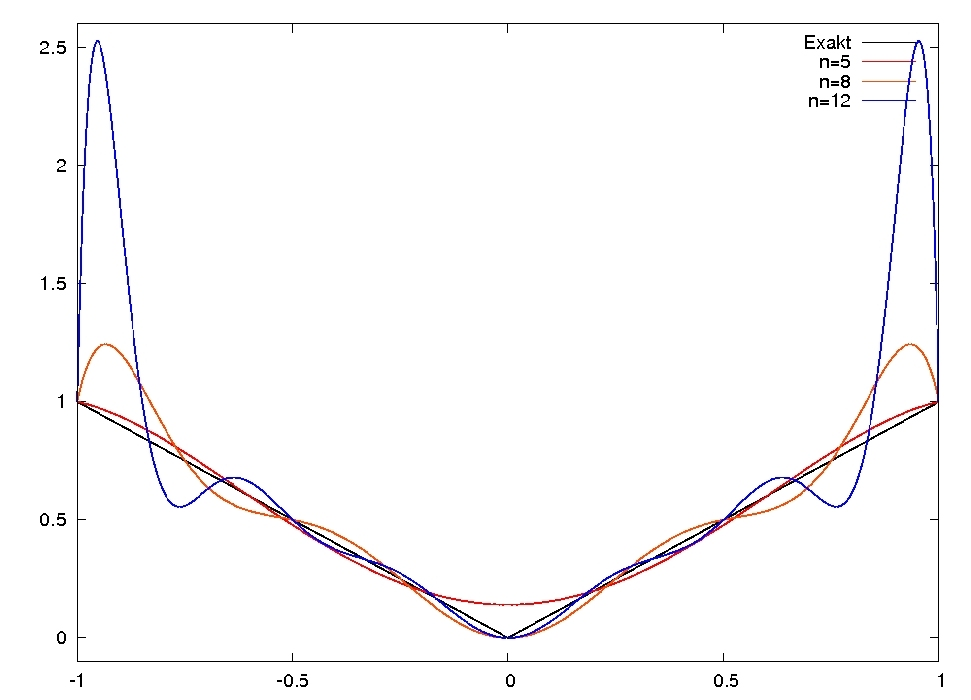
\includegraphics[width=0.5\linewidth]{images/afg49aequi.jpg}
  \caption{Gegenbeispiel zur Konvergenz: äquidistante Gitter für Betragsfunktion}
  \label{6.1.20im1}
\end{figure}
\begin{figure}[t!b]
  \centering
  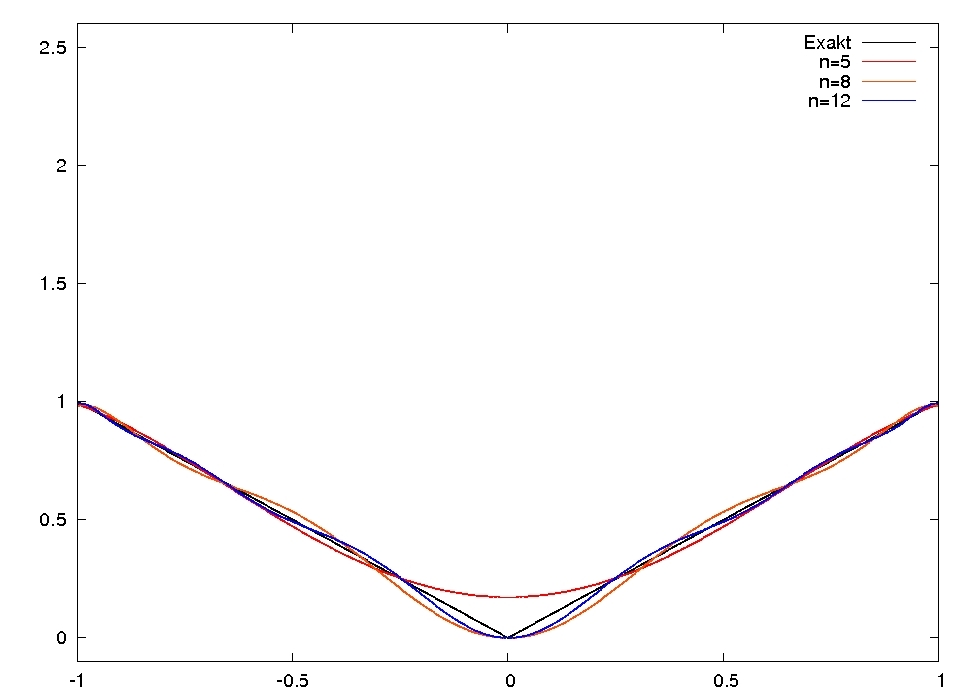
\includegraphics[width=0.5\linewidth]{images/afg49tscheby.jpeg}
  \caption{Gegenbeispiel zur Konvergenz: Tschebyscheff-Punkte für Betragsfunktion}
  \label{6.1.20im2}
\end{figure}

Ein weiteres Gegenbeispiel ist $f(x)=\frac{1}{1+x^2}$ in $[-5,5]$ 
(siehe Übungsaufgabe).

Es gilt sogar:

\begin{Satze}[Faber]
  Zu jeder Folge von Intervalleinteilungen von $[a,b]$
  gibt es eine stetige Funktion $f$ ,
  so dass die Interpolationspolynome auf $[a, b]$
  nicht gleichmäßig gegen $f$ konvergiert 
  (bzgl. $\nn{\,\cdot\,}_\infty$).
\end{Satze}

Basierend auf dem Satz von Jackson gilt:
\begin{Satze}[Konvergenz bei Tschebyscheff-Knoten]
  Sei $f\in C([-1,1])$ Lipschitz-stetig.
  Dann konvergieren die Interpolationspolynome
  zu den Tschebyscheff-Knoten gleichmäßig	gegen $f$ .
\end{Satze}

Andererseits gilt \cite[siehe][]{haemmerlinhoffmann}:
\begin{Satze}[Marcinkiewicz]
  Zu jeder Funktion $f\in C([a,b])$ kann eine Folge von
  Intervalleinteilungen angegeben werden,
  so dass die Folge der Interpolationspolynome gleichmäßig gegen $f$ konvergiert.
\end{Satze}

Im Gegensatz zur $\nn{\,\cdot\,}_\infty$-Norm (auch Tschebyscheff-Norm genannt)
gilt für die $\nn{\,\cdot\,}_2$-Norm \cite[siehe][]{haemmerlinhoffmann}:
\begin{Satze}
  Sei $f\in C([-1,1])$ und seien $x_0,\dots, x_n$ die Nullstellen
  des	Legendre-Polynoms $L_n+1$. Dann gilt
  \begin{gather*}
    \lim\limits_{n\rightarrow \infty}\nn{f-p(f\mid x_0,\dots, x_n)}_2 = 0
  \end{gather*}
\end{Satze}


\sectione{Stückweise polynomiale Approximation durch Splines}
Eine hohe Anzahl von Knoten garantiert keine \enquote{gute}
Approximation durch Interpolationspolynome.
In der Regel treten dann hohe Schwingungen auf,
die unerwünscht sind.
Die Idee der stückweisen polynomialen Approximation ist,
jeweils einige wenige Stützwerte polynomial zu interpolieren
und diese \enquote{glatt} zusammenzusetzen.

% Erste Grafik (Veranschaulichung stückweiser polynomialer Approximation) in 6.2 (Anfang)
\begin{tikzpicture}[>=triangle 45]
  \draw[->,color=black] (0,0) -- (10,0);
  \draw[->,color=black] (0,0) -- (0,8);
  \clip(-0.5,-0.5) rectangle (10,8);
  
  \foreach \x/\text in {0.5/$a=x_0$,3.5/$x_1$,4.5/$x_2$,6/$x_3$,8.5/$x_4=b$}
  \draw (\x,0.1) -- (\x,-0.1) node[below] {\text};
  
  % k=1
  \foreach \x/\y/\wert in {0.5/3.5/4.5,3.5/4.5/1,4.5/6/1.5,6/8.5/5}
  {
    % Waagrechte Linien (chi-Funktionen)
    \draw(\x,\wert)--(\y,\wert);	
    % Beginn und Ende der Linien
    \draw(\x+0.1,\wert-0.2)--(\x,\wert-0.2)--(\x,\wert+0.2)--(\x+0.1,\wert+0.2);	
    \draw (\y-0.1,\wert-0.2) arc (-90:90:0.1 and .2);
  }
  
  % k=2 (linear)
  \foreach \x/\y/\wertx/\werty in {0.5/3.5/4.5/1,3.5/4.5/1/1.5,4.5/6/1.5/5,6/8.5/5/3.5}
  % Gerade zwischen den beiden Punkten
  \draw[color = blue] (\x,\wertx) -- (\y,\werty);
  
  \draw[color=red,smooth,samples=200,domain=0.5:6] plot(\x,{0.058*\x^3-0.073*\x^2-1.696*\x+5.359});
  \draw[color=red,smooth,samples=200,domain=6:8.55] plot(\x,{-0.293*\x^3+4.84*\x^2-24.067*\x+38.52});
\end{tikzpicture}\\
{\centering
  \textit{Veranschaulichung stückweiser polynomialer Approximation}
}
\label{im6.2}

\begin{itemize}
\item stückweise linear und stetig ist am einfachsten
\item stückweise kubisch und global zweimal stetig differenzierbar
  ist zur graphischen Aufarbeitung am geeignetsten,
  da das Auge noch Unstetigkeiten in der Krümmung erkennt.
\end{itemize}


\extrasection{a)}{Splines und zwei verschiedene Basen}
\begin{Defe}\index{Spline}
  Sei $\Delta =\{x_0,\dots,x_n\} $ ein Gitter
  mit paarweise verschiedenen Knoten $a=x_0<\dots<x_n=b$.\\
  Ein (Polynom-)\textbf{Spline von Ordnung $k$}$\geq 2$ 
  (d.h. der Grad der Teilstückpolynome ist maximal $(k-1)$)
  ist eine Funktion $s$ mit $s\in C^{(k-2)}([a,b])$
  und $s\in\p_{k-1}([x_i,x_{i+1}])$
  für $i=0,\dots,n-1$.\\
  Der Raum der Splines von Ornung $k$ bzgl. $\Delta$ sei
  mit $S_{k,\Delta}$ bezeichnet.\\
  Für $k=1$ ist der Raum definiert durch
  \begin{gather*}
    S_{1,\Delta} \coloneqq 
    \left\{
      s:[a,b]\rightarrow\R\,\middle\vert\,
      s|_{[x_i,x_{i+1}]}\in\p_0
      \text{ für } 0\leq i\leq n
    \right\}
  \end{gather*}
  Für $k=2$ ergeben sich \textbf{lineare Splines}\index{Spline!linear}
  und für $k=4$ die \textbf{kubischen Splines}\index{Spline!kubisch}.\\
  Offensichtlich gilt
  \begin{enumerate}[a)]
  \item $S_{k,\Delta}$ ist ein linearer Vektorraum.
  \item $\p_{k-1}\subseteq S_{k,\Delta}$
  \end{enumerate}
  Natürlich lässt sich ein Spline stückweise als Polynom darstellen,
  es hat also $n\cdot k$ Koeffizienten.
  Gewünscht ist aber eine Basisdarstellung,
  welche dann $n+k-1$ Koeffizienten hat.
\end{Defe}

\begin{Satze}\label{6.2.2}\index{abgebrochene Potenz}
  Die Monome $x^l$ und die \textbf{abgebrochenen Potenzen}
  \begin{gather}
    (x-x_i)_+^l\coloneqq
    \begin{cases}
      (x-x_i)^l & x\geq x_i\\
      0         & x<x_i
    \end{cases}
    \label{VI.2.1}
  \end{gather}
  bilden eine Basis\index{Splineraumbasis}
  \begin{gather*}
    \mathcal{B}=
    \left\{
      1,x,\dots,x^{k-1},(x-x_1)+^{k-1},\dots,(x-x_{n-1})_+^{k-1}
    \right\}
  \end{gather*}
  des Splineraumes $S_{k,\Delta}$. Insbesondere gilt
  \begin{gather}
    \dim S_{k,\Delta}=k+n-1
    \label{VI.2.2}
  \end{gather}
  \imagemissing{Dimension eines Splineraumes}\label{im6.2.2}

  \begin{proof}
    siehe Übungsaufgabe
  \end{proof}
\end{Satze}


% --------------------------------------


\subsectione{Nachteile der Splineraumbasis}
\begin{enumerate}[a)]
\item Basisfunktionen haben keine lokalen Träger,
  d.h. zur Auswertung von $s(\overline{x})$ müssen
  alle Basisfunktionen ausgewertet werden, was relativ teuer ist.
\item Falls $x_i\approx x_{i+1}$ sind 
  $(x-x_i)_+^{k-1}$ und $(x-x_{i+1})_+^{k-1}$
  nahezu linear unabhängig.\\
  Damit ist die Basis schlecht konditioniert bzgl. Störungen in $b_i$.
\end{enumerate}

Das Ziel ist nun eine bessere Basis zu konstruieren.

\begin{Bspe}~
  \begin{enumerate}[a)]
  \item \index{Splineraumbasis!$S_{1,\Delta}$-Basis}
    $S_{1,\Delta}$ sind stückweise konstante Funktionen

    % Grafik zu Beispiel 6.2.4
    \begin{tikzpicture}[>=triangle 45]
      \draw[->,color=black] (0,0) -- (10,0);
      \draw[->,color=black] (0,0) -- (0,5);
      \clip(-0.5,-0.5) rectangle (10,5);
      
      \foreach \x/\text in {0.5/$x_0$,3.5/$x_1$,4.5/$x_2$,6/$x_3$,8.5/$x_4$}
      \draw (\x,0.1) -- (\x,-0.1) node[below] {\text};
      
      % k=1
      \foreach \x/\y/\wert in {0.5/3.5/3.5,3.5/4.5/1,4.5/6/1.5}
      {
        % Waagrechte Linien (chi-Funktionen)
        \draw(\x,\wert)--(\y,\wert);	
        % Beginn und Ende der Linien
        \draw(\x+0.1,\wert-0.2)--(\x,\wert-0.2)--(\x,\wert+0.2)--(\x+0.1,\wert+0.2);	
        \draw (\y-0.1,\wert-0.2) arc (-90:90:0.1 and .2);
      }
      
      \draw (6,4)--(8.5,4);
      \draw(6+0.1,4-0.2)--(6,4-0.2)--(6,4+0.2)--(6+0.1,4+0.2);
      \draw(8.5-0.1,4-0.2)--(8.5,4-0.2)--(8.5,4+0.2)--(8.5-0.1,4+0.2);
    \end{tikzpicture}\\
    {\centering
      \textit{Basis eines $S_{1,\Delta}$-Splines aus stückweise
        konstanten Elementen}
    }
    \label{im6.2.4(1)}

    Die zugehörige Basis wie oben beschrieben wäre
    \begin{gather*}
      \left\{ 1,(x-x_i)_+^0\right\}
    \end{gather*}
    Eine in diesem Fall geeignetere Basis ist
    \begin{gather*}
      N_{i,1} (x)\coloneqq \chi_{[x_{i-1},x_i)}(x)
      = \begin{cases}
        1 & \text{falls } x\in[x_{i-1},x_i)\\
        0 & \text{sonst}
      \end{cases}\, ,
    \end{gather*}
    womit die Darstellung eines $S_{1,\Delta}$-Splines zu 
    \begin{gather*}
      s(x) = \sum_{j=1}^{n+1} f_{j-1} N_{j,1}(x)
    \end{gather*}
    wird.
  \item \index{Splineraumbasis!$S_{2,\Delta}$-Basis} $S_{2,\Delta}$ sind stückweise lineare, global stetige
    Funktionen. Eine Basis wie in \ref{6.2.2} ist
    \begin{gather*}
      \left\{1,x^1, (x-x_i)_+^1\right\}
    \end{gather*}
    \imagemissing{Basis eines $S_{2,\Delta}$-Splines mit Hutfunktion
      (siehe auch \ref{6.2.6} für allg. Hutfunktionen)}\label{im6.2.4(2)}
    Hier kann eine Basis wie oben durch sog. 
    \textbf{Hutfunktionen}\index{Hutfunktion}
    konstruiert werden
    \begin{align*}
      N_{i,2}(x_{j-1}) &= \delta_{i,j}\\
      N_{i,2}(x) &= \begin{cases}
        ~\frac{1}{x_{i-1}-x_{i-2}}(x-x_{i-2}) & x\in [x_{i-2}, x_{i-1}]\\
        -\frac{1}{x_{i-1}-x_{i-2}}(x-x_{i-1})+1 & x\in [x_{i-1}, x_i]
      \end{cases}
    \end{align*}
    \imagemissing{allgemeine Hutfunktion am Punkt $x_i$ eines
      $S_{2,\Delta}$-Splines}\label{im6.2.4(3)}
    Ein Spline, welches $f$ in $x_i$ interpoliert hat dann die Form
    \begin{gather*}
      s(x) = \sum_{j=1}^{n+1}f_{j-1}N_{j,2}(x)
    \end{gather*}
  \end{enumerate}
\end{Bspe}


\begin{Defe}
  Sei $t_1\leq \dots \leq t_m$ eine beliebige Folge von Knoten
  $x_i$.\\
  Dann sind die \textbf{B-Splines}\index{Spline!B-Splines}
  $N_{j,l}$ für $l=1,\dots, m$ und $j=1,\dots, m-l$ 
  rekursiv erklärt durch
  \begin{align}\nonumber
    N_{j,1}(x) &\coloneqq \chi_{[t_j,t_{j+1})}(x) 
                 \text{ für } t_{j+1}\neq t_j\\
    N_{p,1}(x) &= \chi_{[t_p,t_m]}(x) 
                 \text{ für }
                 p=\min\left\{i\,\middle\vert\,t_{i+1}=t_m\right\}
                 \label{VI.2.3}
  \end{align}
  sowie für $l>1$
  \begin{gather}
    N_{j,l} (x) = \frac{x-t_j}{t_{j+l-1}-t_j}N_{j,l-1}(x) 
    +  \frac{t_{j+l}-x}{t_{j+l}-t_{j+1}}N_{j+1,l-1}(x) 
    \label{VI.2.4}
  \end{gather}
  Hierbei gilt die Konvention $\frac{0}{0}=0$, 
  denn für $t_j=t_{j+l-1}$ gilt
  $N_{j,1}\equiv 0$ und auch $N_{j,l-1}\equiv 0$.
\end{Defe}


Ziel ist nun u.a. mit diesem eine Basis von $S_{k,\Delta}$ anzugeben,
die zudem gut konditioniert ist.
Vorher jedoch werden noch einige Eigenschaften der B-Splines
untersucht.


\subsectione{Gestalt der B-Splines}\label{6.2.6}
Bei einem B-Spline $N_{j,k}$ entspricht $j$ dem Ort und
$k-1$ entspricht dem Polynomgrad.

{\centering
  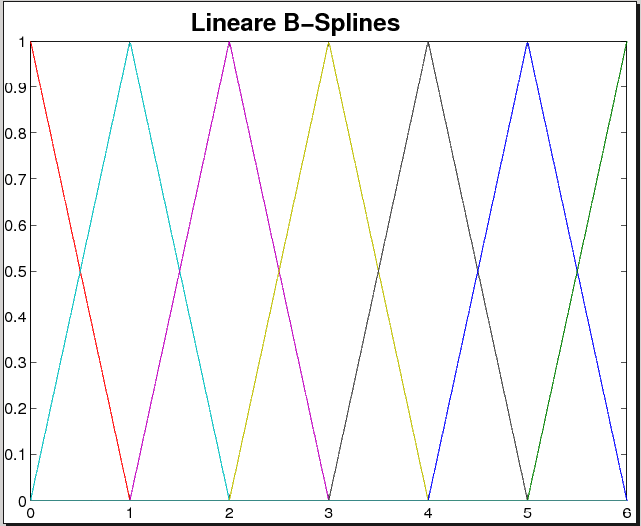
\includegraphics[width=\linewidth]{images/linBsplines.png}

  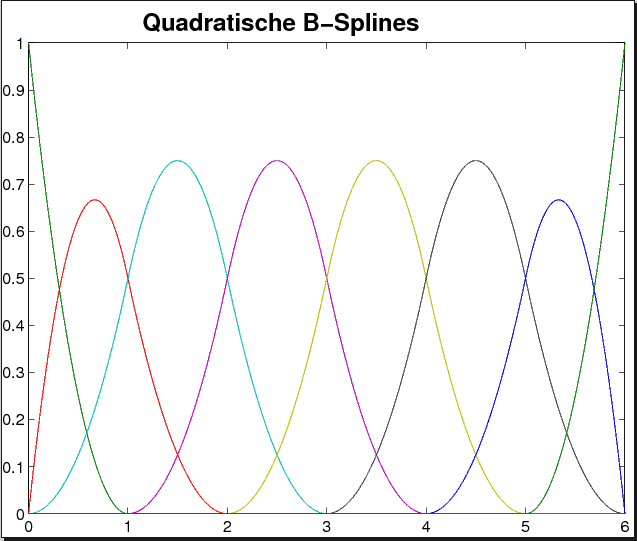
\includegraphics[width=\linewidth]{images/quadBsplines.png}

  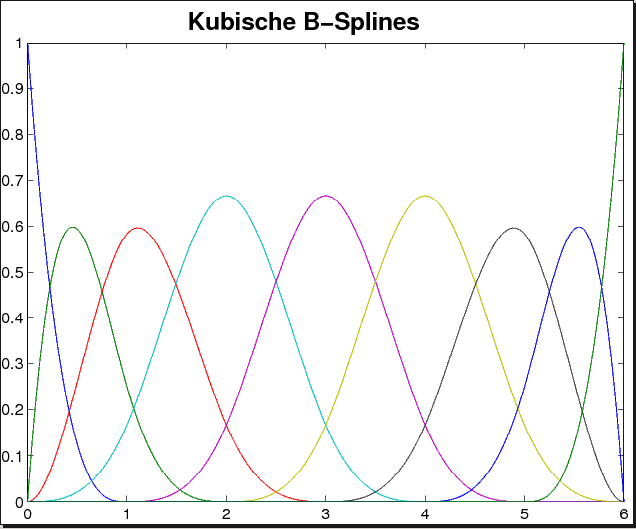
\includegraphics[width=\linewidth]{images/kubBsplines.png}
}

\begin{Kore}
  Es gilt
  \begin{enumerate}[a)]
  \item $supp N_{j,k} \coloneqq 
    \overline{\left\{ x\in[a,b]\,\middle\vert
        \, N_{j,k}(x)\neq 0\right\}} \subset [t_j, t_{j+1}]$
    (lokaler Träger)
  \item $N_{j,k}>0 ~\forall x\in(t_j,t_{j+1})$ (nicht negativ)
  \item $N_{j,k}\vert_{[t_l,t_{l+1})}\in \p_{k-1}$
  \end{enumerate}

  \begin{proof}
    siehe Übungsaufgabe
  \end{proof}
\end{Kore}

\subsectione{Auswertung von $s$ an der Stelle $\overline{x}$}
\label{6.2.8}
Sei $\overline{x}\in[t_j,t_{j+1}]$ und
$s(x) = \sum_{i=1}^{N}c_iN_{i,k}(x)$.
Da nur $N_{j,1}(\overline{x})\neq 0$ ist, 
können aufgrund von \eqref{VI.2.4}
auch nur $N_{j-k+1, k}(\overline{x}), \dots, N_{j,k}(\overline{x})$
verschieden von Null sein, da
\begin{align*}
  \begin{array}{ccccccccc}
    j\backslash l & t_j & 1 && 2 && 3 &&k\\
    \cline{1-9}
    1 & t_1 & N_{1,1}(\overline{x})=0 &&0&&0&&0\\
                  &&0&&\vdots&&\vdots&&\vdots\\
                  &&\vdots &&&&&&0\\
    j-k+1&t_{j-k+1} &\dots &&\dots&&\dots&&\boldsymbol{N_{j-k+1,k}(\overline{x})} \\
    \vdots&\vdots&&&&&&&\vdots\\
                  && &&0&& \boldsymbol{N_{j-2,3}(\overline{x})}
                                 &&N_{j-2,k}(\overline{x})\\
    j-1 & t_{j-1} &0 &\longrightarrow & \boldsymbol{N_{j-1,2}(\overline{x})}
                                      &\longrightarrow & N_{j-1,3}(\overline{x})
            && N_{j-1,k}(\overline{x})\\
    j& t_j & \boldsymbol{N_{j,1}(\overline{x})=1}&\longrightarrow&\boldsymbol{N_{j,2}(\overline{x})}
                                      &\longrightarrow&\boldsymbol{N_{j,3}(\overline{x})}&\longrightarrow\dots&\boldsymbol{N_{j,k}(\overline{x})}\\
                  &&0&&0&&&&\vdots\\
                  &&\vdots &&\vdots\\
                  &t_{j+k}&0&&0&&&&0
  \end{array}
\end{align*}

Daraus folgt, dass $N_{i,k}(\overline{x})\neq x$ 
für höchstens $i=j-k+1,\dots, j$.\\
Nach der Rekursionsformel baut $N_{i,k}$ auf 
$N_{i,1},\dots , N_{i+(k-1),1}$ auf und
benutzt $t_i,\dots, t_{i+k}$.\\
Da in der Rekursionsformel nur nichtnegative Vielfache
nichtnegativer Zahlen addiert werden,
ist das Verfahren zur Bestimmung der $N_{i,k}(\overline{x})$
numerisch sehr stabil.

\begin{Leme}
  Falls $t_j<t_{j+k}$ und $x\neq t_m$,
  so gilt
  \begin{gather}
    N_{j,k}(\overline{x})=(t_{j+k}-t_j)\underset{
      [t_j,\dots, t_{j+k}]f\text{ mit } f(t)\coloneqq (t-x)_+^{k-1}}
    {[t_j,\dots,t_{j+k}](\bullet -x)_+^{k-1}}
    \label{VI.2.5}
  \end{gather}
\end{Leme}

\begin{proof}
  kein Beweis.

  Idee: Per Induktion über $k$. Nutze hierfür
  \begin{gather*}
    (t-x)_{+}^k = (t-x)(t-x)_{+}^{k-1}\,,\, k \geq 1,
  \end{gather*}
  sowie $[t_j , \dotsc, t_i]( \bullet - x) = 0$ für $i > j+1$ und die Leibnizregel.
\end{proof}

Zu gegebenem Splineraum $S_{j,\Delta}$ mit
% Nummerierung
\begin{gather}
  \Delta a=x_0 < x_1 < \dotsm < x_n = b
  \label{VI.2.6}
\end{gather}
Setzt man nun 
\begin{gather}
  T: t_1 = \dotsm = t_k < t_{k+1} < \dotsm < t_{k+n} =
  t_{n+2k+1}\, ,
  \label{VI.2.7}
\end{gather} lässt sich folgender Satz zeigen:


% --------------------------------


\begin{Satze}\label{6.2.10}~
  \marginpar{17.12.2014}
  \begin{enumerate}
  \item Es gilt 
    $\p_{k-1}\subset
    span\left\{N_{1,k}, \dots, N_{n+k-1,k}\right\}$
  \item Die B-Splines bilden eine Zerlegung der Eins auf $[a,b]$,
    d.h. 
    \begin{gather*}
      1\equiv \sum_{j=1}^{n+k-1}N_{j,k}(x) \quad \forall x\in[a,b]
    \end{gather*}
  \item Weiterhin sind die B-Splines (lokal) linear unabhängig,
    d.h. falls
    \begin{gather*}
      \sum_{l=1}^{n+k-1}c_lN_{l,k}(x)=0 
      \quad\forall x\in(c,d)\subset [a,b]\,,
    \end{gather*}
    folgt $c_j=0$ für alle $j$ mit 
    $(c,d)\cap \underbrace{(t_j,t_j+k)}_{=supp N_{j,k}}\neq \varnothing$.
    \imagemissing{Lineare Unabhängigkeit der B-Splines}\label{im6.2.10}
  \end{enumerate}

  \begin{proof}~
    \begin{description}
    \item[a), b)] folgen aus der Marschen-Identität 
      \cite[siehe z.B.][]{deuflhardhohmann}
    \item[c)] O.B.d.A. enthalte $(c,d)$ keine Knoten $t_i$
      (sonst zerlege $(c,d)$ in Teilintervalle).
      Dann folgt $(c,d)\subseteq (t_l, t_{l+1})$.
      Nach a) lässt sich jedes Polynom $p\in \p_{k-1}$
      durch die B-Splines $N_{l,k}$ darstellen.
      Auf $(c,d)$ sind nur $k=dim\p_{k-1}$
      B-Splines von Null verschieden.
      Daher müssen diese linear unabhängig sein.
    \end{description}
  \end{proof}
\end{Satze}

\begin{Fole}
  Die B-Splines $\{N_{1,k},\ldots,N_{n+k-1,k}\}$ bilden eine Basis von 
  $S_{k,\Delta}$.

  Die Koeffizienten $c_i$ der Basisdarstellung von $s \in S_{k,\Delta}$
  \begin{gather*}
    s(x)=\sum_{i=1}^{n+k-1}c_iN_{ik}(x)
  \end{gather*}
  heißen \textbf{de Boor-Punkte}\index{de Boor-Punkte} von $s$. \\
  Die Funktionswerte $s(x)$ sind somit eine
  Konvexkombination der de Boor-Punkte $c_i$.
\end{Fole}


\begin{Beme}
  Die B-Spline Basis ist eine gut konditionierte Basis, d.h.
  die Auswertung von Splines mittels ihrer B-Spline
  Darstellung ist gut konditioniert.
  Es gilt mit $N\coloneqq n+k-1$
  \begin{gather*}
    D_k \max_{j=1,\ldots, N} |c_j| 
    \leq \nn{\sum^N_{j=1} c_j N_{jk}}_{\infty}
    \leq \max_{j=1,\ldots, N} | c_j|
  \end{gather*}
  Die Konstante $D_k$ hängt nur von der Ordnung $k$ ab, nicht
  von der Lage der Knoten.
\end{Beme}

\extrasection{b)}{Splineinterpolation}

\subsectione{Splineinterpolation allgemein}\label{6.2.13}
Gegeben seien $N=n+k-1=dimS_{k,\Delta}$ Stützpunkte $(\xi_i,f_i)$
mit
\begin{gather*}
  \xi_1<\dots<\xi_N\,.
\end{gather*}
Gesucht sind nun Splines $s\in S_{k,\Delta}$ 
mit $s(\xi_i)=f_i$ für alle $i=1, \dots, N$.
Das ist äquivalent zu 
\begin{align}
  \sum_{j=1}^N c_jN_{j,k}(\xi_i)&=f_i &&\text{für }i=1,\dots, N
                                         \label{VI.2.8}
  \\\nonumber
  \Leftrightarrow Ac&=f &&\text{mit } A=(N_{j,k}(\xi_i))_{i,j=1,\dots,N}
\end{align}

\subsectione{Lineare B-Splines}\label{6.2.14}
Sei $k=2$, $N=n+1$, $S_{2,\Delta}$ der Splineraum zu einem $\Delta$,
welches konstruiert werden soll.
\imagemissing{Stützstellen für eine konstruierte Zerlegung $\Delta$}\label{im6.2.14}
Sei $x_0\coloneqq \xi_1<x_1\coloneqq \xi_2<\dots<x_n\coloneqq
\xi_{n+1}$, dann folgt
\begin{gather*}
  N_{i,2}(\xi_j)=N_{i,2}(t_{j+1})=\delta_{i,j}
\end{gather*}
Also ist in diesem Fall die Matrix $A=(N_{j,k}(\xi_i))_{i,j\leq n}=I$
also $c_i=f_i=f(\xi_i)=f(x_{i-1})$.
Der zugehörige Spline $s$ hat dann die Form
\begin{align*}
  s(x) &= \sum_{i=1}^{N}f_i N_{i,2}(x) \\
       &= \sum_{j=0}^{N}f(x_j)N_{j+1,2}(x)
\end{align*}
Zur Auswertung von $s$ wird \ref{6.2.8} verwendet.
$A$ sei definiert als
\begin{gather*}
  A \coloneqq \left(N_{j,k}(\xi_i)\right)_{i,j=1,\ldots,N}
\end{gather*}
und hat folgende Eigenschaften
\begin{itemize}
\item  $A$ besitzt Bandstruktur, da  $\xi_i$ höchstens in $k$
  Intervallen $[t_j, t_{j+k}]$ liegen kann.
\item $A$ ist regulär, also $N_{ik}(\xi_i)\neq 0$
  für $i=1, \ldots, N$.\\
  (nach dem Satz von Schoenberg und Whitney, 1953)
\item $A$ ist total positiv, d.h. für alle quadratischen
  Untermatrizen $B$ gilt $\det(B)\geq 0$.\\    
  (nach Karlin, 1968)
\end{itemize}

Daraus kann man folgern, dass
die Gaußelimination für Bandmatrizen ohne Pivotsuche
durchführbar ist, falls $N_{ik}(\xi_i) \neq 0$
für $i =1, \ldots, N$.\\


\subsectione{Kubische B-Spline-Interpolation} \label{6.2.15}
Sei $k=4$ und entsprechend $N=n+3$ und 
seien die Stützpunkte zur Interpolation wie in \ref{6.2.14}
gegeben durch 
\begin{gather*}
  \xi_i = x_{i-1} \quad \text{ für } i=1, \ldots, n+1\,.
\end{gather*}
(Daraus folgt $N\neq n+3$ und \ref{6.2.13} ist nicht anwendbar.)\\
Zur eindeutigen Bestimmung von $s\in S_{4,\Delta}$ fehlen zwei
Bedingungen.\\
Typischerweise werden 
zusätzlich zu 
\begin{gather*}
  s(x_i)=f(x_i) \quad \text{für } i=0,\ldots,n
\end{gather*} 
eine der folgenden Randbedingungen gefordert:
\begin{enumerate}[i)]
\item $s'(a)=f'(a)$ und $s'(b)=f'(b)$:  \\
  \textbf{vollständige} oder \textbf{Hermitesche kubische 
    Spline-Interpolation} 
\item $s''(a)=s''(b)=0$ (\enquote{natürliche}  Endbedingungen):\\
  \textbf{natürliche kubische Spline-Interpolation}\\
  (d.h. $s$ kann linear außerhalb von $[a,b]$ glatt fortgesetzt
  werden) 
\item $s'(a)=s'(b)$ und $s''(a)=s''(b)$,
  falls $f$ periodisch mit Periode $b-a$ ist: \\
  \textbf{periodische kubische Spline-Interpolation}.
\end{enumerate}
Die drei Randbedingungen werden aufgrund physikalischer
Eigenschaften gefordert. Hierzu ein Beispiel: 

Es beschreibe $y(t)$ die Lage eines
homogenen, isotropen Stabes (z.B. eine dünne Holzlatte).
Dann misst
\begin{gather*}
  E(y) = c \int_a^b\left(
    \frac{y''(t)}{(1+y'(t)^2)^{\frac{3}{2}}}
  \right)^2dt
  = c \int_a^b\left(
    \kappa(t)
  \right)^2dt
\end{gather*}
(wobei $\kappa $ die Krümmung der Kurve $y$ in der Ebene ist) 
die Biegeenergie.\\
Aufgrund des \textbf{Hamiltonschen Prinzips}\index{Hamiltonsches Prinzip}
stellt sich der Stab so ein, dass $E(y)$ minimiert wird.\\
Unter der Annahme $|y'(t)| \ll 1$ für $t\in [a,b]$ 
wird $E$ linearisiert zu $c\int_a^by''(t)^2dt$.
Also wird annähernd eine Funktion $y\in C^2$ gesucht,
welche $\nn{y''}_2^2$ minimiert.

Obige Splines haben gerade diese Eigenschaft, denn:

\begin{Satze}\label{6.2.16}
  Sei $s$ ein interpolierender, kubischer Spline von $f$
  in den Knoten $x_i $ und $y\in C^2$ eine beliebige Funktion
  von $f$, so dass 
  \begin{gather*}
    \left[s''(t)\cdot(y'(t)-s'(t))\right]_{t=a}^{b}=0
  \end{gather*}
  Dann gilt $\nn{s''}_2 \leq \nn{y''}_2$.

  \begin{proof}
    Es gilt
    \begin{align*}
      \nn{y''}_2^2 &= \nn{s''+(y''-s'')}_2^2\\
                   &= \nn{s''}_2^2
                     + 2\underbrace{\int_{a}{b}s''(y''-x'')dt}_{
                     \mathclap{\substack{=0 \\ \text{ wie gezeigt wird}}}
      }
      + \nn{y''-s''}_2^2
    \end{align*}
    da
    \begin{align*}
      \int_{a}^{b} s''(y''-x'')dt &= \sum_{i=1}^{N}\left(\left[
                                    s''(y'-s')\right]_{x_{i-1}}^{x_i}
                                    -\int_{x_{i-1}}^{x_i}s'''(y'-s')dt\right)\\
      \intertext{($S_{4,\Delta}\subseteq C^2([a,b])$, 
      $s'''(x)\equiv d_{i-1}=const$, 
      da 
      $s\in\p_3([x_{i-1},x_i])$ )
      }
                                  &= \underbrace{\left[ s''(y'-s')\right]_{a}^{b}}_{
                                    \mathclap{\substack{ =0 \\ \text{ nach Voraussetzung } }}
      }
      -\sum_{i=1}^{N} d_{i-1}
      \int_{x_{i-1}}^{x_i} \left(y'(t)-s'(t)\right) dt\\
                                  &=-\sum_{i=1}^N d_{i-1}\bigg(\big(y(x_i)-s(x_i)\big)
                                    - \big(y(x_{i-1})-s(x_{i-1})\big)\bigg) \\
                                  &=0
    \end{align*}
    da $y$,$s$ Interpolationen von $f$ sind.\\
    Mit den Randbedingungen i), ii) und iii) 
    ist die Voraussetzung von \ref{6.2.16} erfüllt.
  \end{proof}
\end{Satze}

\begin{Kore}\label{6.2.17}
  Es existiert genau ein interpolierender kubischer Spline 
  $s\in S_{4,\Delta}$, welcher die Randbedingungen aus \ref{6.2.16}
  erfüllt.
  Weiterhin gilt für jede interpolierende Funktion $y\in C^2([a,b])$,
  die derselben Randbedingung genügt
  \begin{gather*}
    \nn{s''}_2 \leq \nn{y''}_2
  \end{gather*}

  \begin{proof}
    Die Anzahl der Forderungen ist $N=dim S_{4,\Delta}$.
    Es ergibt sich also ein quadradratisches lineares Gleichungssystem
    und es genügt Injektivität zu zeigen.\\
    Sei $f\equiv 0$, dann erfüllt $y\equiv 0$ alle Forderungen.
    für alle Lösungen $s\in S_{4,\Delta}$ gilt daher
    \begin{gather*}
      \nn{s''}_2\leq \nn{y''}_2 =0 \quad \text{ nach \ref{6.2.16}}
    \end{gather*}
    Also gilt $s''\equiv 0$ und $s$ ist stückweise kubische Funktion
    mit $s\in C^2([a,b])$  und $s(x_i)=0$.
    Damit folgt $s\equiv 0$, was die Injektivität zeigt.
  \end{proof}
\end{Kore}

% ----------------------------------------------------


\subsectione{Berechnung der natürlichen Splines mittels B-Splines}
\label{5.2.18}
\marginpar{22.12.2014}
\begin{gather*}
  A \coloneqq 
  \left(\begin{array}{ccccccccc}
          \frac{x_2+x_1-2x_0}{x_2-x_0}& & -\frac{x_1-x_0}{x_2-x_0}& && & & & \\
          N_{2,4}(x_1)&&N_{3,4}(x_1) &&N_{4,4}(x_1)  & &&&0 \\
                                      &\ddots & &\ddots& &\ddots &  &&\\
                                      & & N_{i+1,4}(x_i)&& N_{i+2,4}(x_i) && N_{i+3,4}(x_i) && \\
                                      & &  &\ddots& &\ddots &&\ddots  &\\
          0&&&  &N_{n,4}(x_{n-1}) &&N_{n+1,4}(x_{n-1}) &&N_{n+2,4}(x_{n-1}) \\
                                      & & && && -\frac{x_n-x_{n-1}}{x_n-x_{n-2}} && \frac{2
                                                                                    x_n-x_{n-2}-x_{n-1}}{x_n-x_{n-2}}
        \end{array}\right)
    \end{gather*}
    Die Werte $N_{j,4}(x_i)$ lassen sich nach \ref{6.2.8} berechnen.


    Insbesondere ergibt sich für äquidistantes Gitter
    \begin{equation*}
      \frac{1}{12}
      \left(\begin{array}{ccccccc}
              18& -6&&&&&\\
              3&7&2&  &&&\\
                &2&8&2  &&&\\
                & &\ddots &\ddots &\ddots &&\\
                & & & 2&8&2&\\
                & & & &2&7&3\\
                & & &&&-6&18\\
            \end{array}\right) 
          \left(\begin{array}{c}
                  c_2\\ \\ \vdots \\ \\c_{n+2}
                \end{array}\right)
              =
              \left(\begin{array}{c}
                      f_0\\ \\ \vdots \\ \\f_n
                    \end{array}\right)
                \end{equation*}
                (siehe Übung).


                \begin{Bspe}[Laster]\label{5.2.20}
                  Das folgende Beispiel zeigt,
                  dass sowohl die Glattheit der Funktion
                  wie auch die Knotenverteilung einen Einfluß hat,
                  da die zugehörige Funktion nicht differenzierbar ist,
                  bzw. die Ableitungen betragsmäßig sehr groß sind.

                  Natürliche Spline-Interpolation
                  versus polynomiale Interpolation:\\
                  {\centering
                    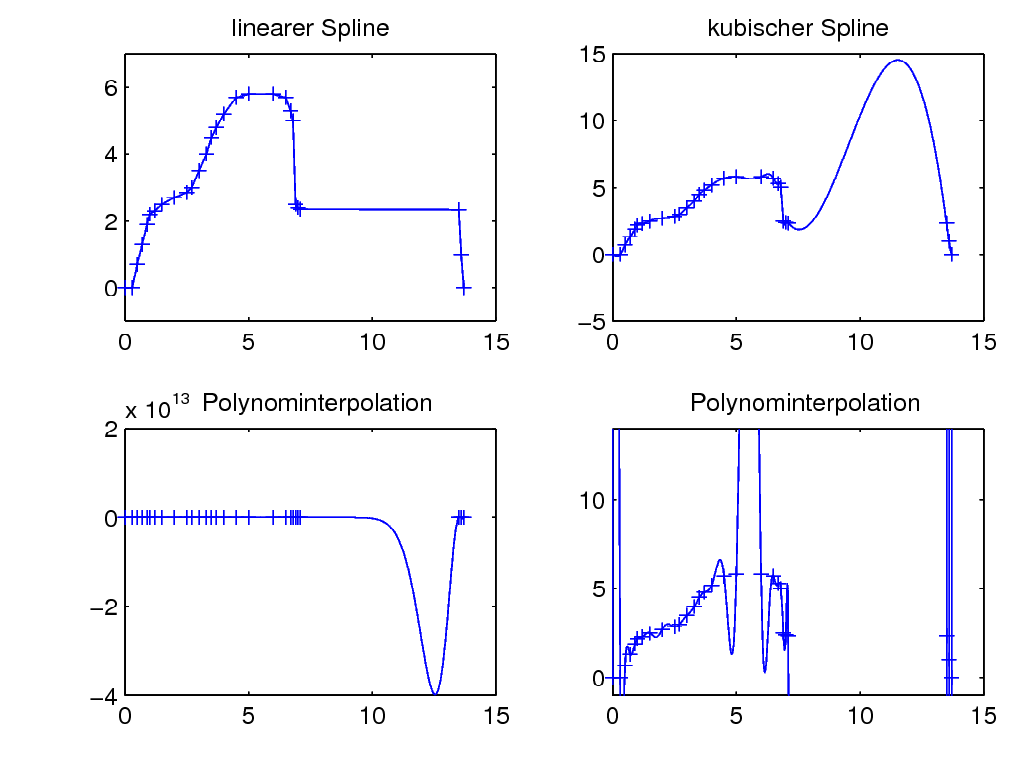
\includegraphics[width=\linewidth]{images/laster1.png}
                  }

                  Mit mehr Stützstellen:\\
                  {\centering
                    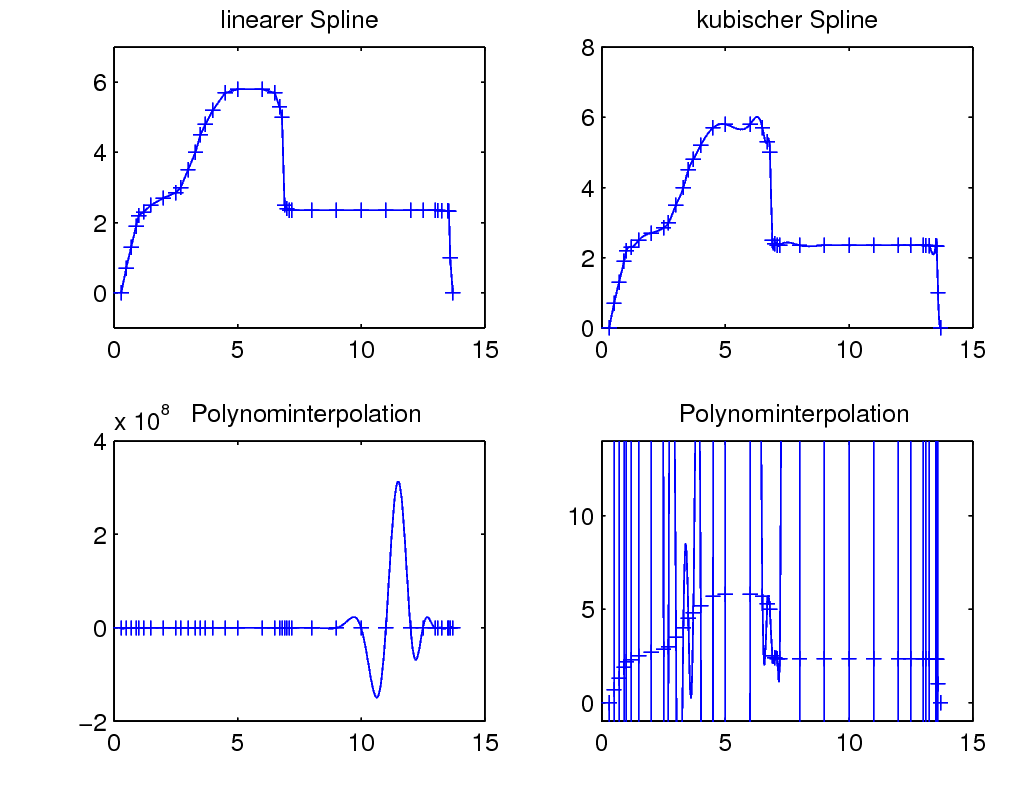
\includegraphics[width=\linewidth]{images/laster2.png} 
                  }
                \end{Bspe}

                \begin{Satze}[Fehlerabschätzung für kubische Splines]\label{5.2.21}
                  Sei $f\in C^4([a,b])$ und $s\in S_{4,\Delta}$ 
                  der interpolierende, vollständige, kubische Spline 
                  zu äquidistanten Knoten mit $h=x_{i+1}-x_i$. Dann gilt
                  für $k=0,1,2,3$
                  \begin{gather*}
                    \nn{f^{(k)}-s^{(k)}}_{\infty}\leq c_kh^{4-k}\nn{f^{(4)}}_{\infty}
                  \end{gather*}
                  mit $c_0=\frac{5}{384}$, $c_1=\frac{1}{24}$, $c_2=\frac{3}{8}$,
                  $c_3=1$, wobei $c_0$ und $c_1$ optimal sind.

                  \begin{proof}
                    \cite[siehe z.B.]
                    [(in allgemeiner Form, d.h. auch für nicht gleichmäßiges Gitter)]
                    {stoerbulirsch}\\
                    Die optimalen $c_k$ wurden von Hall und Meyer (1976) bewiesen.
                    Oft wird mit Stetigkeitsmodulen gearbeitet.
                  \end{proof}
                \end{Satze}


                Für eine wachsende Anzahl der Knoten ergibt sich also Konvergenz,
                anders als bei polynomialer Interpolation.


                \begin{Satze}[Fehlerabschätzung für lineare Splines]\label{6.2.22}
                  Sei $f\in C^2([a,b])$ und $s\in S_{2,\Delta}$
                  der interpolierende Spline  an den Stützstellen 
                  $a=x_0<x_1<\ldots<x_n=b$. 
                  Dann gilt mit $h=max_{i=0,\ldots,n-1}|x_{i+1}-x_i|$
                  \begin{gather*}
                    \nn{f-s}_{\infty}\leq \frac{h^2}{8}\nn{f''}_{\infty} \, .
                  \end{gather*}

                  \begin{proof} 
                    siehe Übungsaufgabe
                  \end{proof}
                \end{Satze}


                Weitere Literatur zu
                Splines: \cite{boor}


% Kap. 7: Numerische Integration/Quadratur}
% % % % % % % % % % % % % % 
% 
% Skript zu NUMERIK I
% WS14/15
% von Prof. Dr. Blank
% Universität Regensburg
% 
% 
%	Kap. 7: Numerische Integration/Quadratur
% 
% % % % % % % % % % % % % % 



\chapter{Numerische Integration/Quadratur}


\sectione{Einführung und einfache Quadraturformeln}
Häufig sind Integrale
\begin{gather*}
  I(f) \coloneqq \int_a^bf(t)dt
\end{gather*}
nicht analytisch zu berechnen
oder die benötigte analytische Darstellung
des unbestimmten Integrals ist kompliziert.
Ziel ist $I(f)$ durch eine 
\textbf{Numerische Quadratur}\index{Numerische Quadratur}
\begin{gather*}
  \hat{I}(f)
\end{gather*}
zu approximieren.

Der Begriff numerische Integration ist allgemeiner und
beschreibt das numerische Lösen von
\begin{gather*}
  y'(t) = f\big(t,y(t)\big) \qquad \text{mit } y(a)=c
\end{gather*}
Die numersiche Quadratur $\hat{I}(f)$ sollte
\begin{enumerate}[a)]
\item effizient ausführbar sein,
\item viele Eigenschaften der Integration beibehalten und
\item $I(f)$ gut approximieren.
\end{enumerate}
Zu c) einige Eigenschaften des Riemann-Integrals:\\
Seien $f,g\in C([a,b])$, dann ist $I:C([a,b])\longrightarrow\R$
eine positive Linearform, d.h. $I$ ist linear und 
\begin{gather}
  f\geq 0 \quad \Rightarrow \quad I(f)\geq 0
  \label{VII.1.1}
\end{gather}
Weiterhin gilt
\begin{gather}
  \int_a^b f(t)dt + \int_b^c f(t)dt = \int_a^cf(t)dt
  \label{VII.1.2}
\end{gather}
Diese sollen nun möglichst beibehalten werden.

\begin{Defe}\label{7.1.1}
  Ein Verfahren heißt konvergent von der Ordnung $p$
  (hat die Konvergenzordnung $p$),
  falls der Fehler (hier $|I(f)-\hat{I}(f)|$)
  mit $\mathcal{O}(h^p)$ gegen Null geht für $h\longrightarrow 0$.
\end{Defe}

\subsectione{Mittelpunktregel}
\imagemissing{Veranschaulichung der Mittelpunktregel}\label{im7.1.2}
Zerlege $[a,b]$ in Teilintervalle $[x_i,x_{i+1}]$
für $i=0,\dots,n-1$ der Länge $h_i=x_{i+1}-x_i$, d.h.
\begin{gather*}
  a=x_0 < x_1 < \dots < x_n = b
\end{gather*}
und setze zur Approximation von $I(f)$
\begin{gather}
  \hat{I}_M(f) \coloneqq \sum_{i=0}^{n-1}f\left(
    \frac{x_{i+1}+x_i}{2}
  \right)
  \cdot (x_{i+1}-x_i)
  \label{VII.1.3}
\end{gather}
Für ein äquidistantes Gitter ergibt sich mit $h=\frac{b-a}{n}$
\begin{gather}
  \hat{I}_M(f)= h \sum_{i=0}^{n-1}f\left(
    x_{i}+\frac{h}{2}
  \right)
  \label{VII.1.4}
\end{gather}
Die \textbf{Fehlerschranke}\index{Fehlerschranke}
(Konvergenzordnung) für $f\in C^2([a,b])$
\begin{gather}
  \left| I(f) -\hat{I}_M(f)\right|
  \leq \frac{h^2}{24}(b-a)\nn[f'']_\infty
  \label{VII.1.5}
\end{gather}
ergibt sich aus der Taylorentwicklung
\begin{gather*}
  f(t) = f\left(x_i+\frac{h}{2}\right)
  + f'\left(x_i+\frac{h}{2}\right) \cdot 
  \left(t-\left(x_i+\frac{h}{2}\right)\right)
  + \frac{1}{2}f''\big(\xi_i(t)\big)\cdot
  \left(t-\left(x_i+\frac{h}{2}\right)\right)^2
\end{gather*}
mit einer Zwischenstelle $\xi_i(t)$ zwischen $t$ und
$\left(x_i+\frac{h}{2}\right)$, denn
\begin{align*}
  \left|I(f)-\hat{I}_M(f)\right|
  &\leq \sum_{i=0}^{n-1} \left|
    \int_{x_i}^{x_{i+1}}f(t)dt - h\cdot f\left(x_i+\frac{h}{2}\right)
    \right|\\
  &=\sum_{i=0}^{n-1} \left|
    \int_{x_i}^{x_{i+1}}\left( 
    f(t) - f\left(x_i+\frac{h}{2}\right)
    \right) dt
    \right|
    \intertext{da $\int_{x_i}^{x_{i+1}}\left(t-\left(x_i+\frac{h}{2}\right)\right)dt=0$}
  &= \sum_{i=0}^{n-1} \left|
    \int_{x_i}^{x_{i+1}}
    \frac{1}{2} f''\big(\xi_i(t)\big)
    \cdot \left(t-\left(x_i+\frac{h}{2}\right)\right)^2dt
    \right|\\
  &\leq \nn[f'']_\infty \cdot \frac{1}{2}
    \sum_{i=0}^{n-1}
    \int_{x_i}^{x_{i+1}}
    \left(t-\left(x_i+\frac{h}{2}\right)\right)^2dt\\
  &=\frac{h^2}{24} (b-a)\nn[f'']_\infty
\end{align*}
Für andere Interpolationspunkte als den Mittelpunkt 
(z.B. einer der Eckpunkt) wird $\mathcal{O}(h^2)$, d.h. 
die Ordnung $2$, nicht erreicht.

\subsectione{Trapezsumme}\index{Trapezregel}
Interpoliere stückweise linear
\imagemissing{Veranschaulichung Trapezsumme}\label{im7.1.3}
\begin{align}\nonumber
  &(x_{i+1}-x_i)\cdot \frac{f(x_i)+f(x_{i+1})}{2} 
  &\text{(Trapezregel)}\\
  \Rightarrow\quad
  & \hat{I}_T(f) = \frac{1}{2}\sum_{i=0}^{n-1}
    \big(
    f(x_i)+f(x_{i+1})
    \big)
    \cdot (x_{i+1}-x_i)
    \label{VII.1.6}
\end{align}
und für äquidistante Gitter ergibt sich die \textbf{Trapezsumme}
\begin{gather}
  \hat{I}_T(f) = h\cdot\left( \frac{1}{2}f(x_0)
    +\sum_{i=0}^{n-1}f(x_i)
    +\frac{1}{2} f(x_n)
  \right)
  \label{VII.1.7}
\end{gather}
Die Konvergenz folgt durch die Riemannschen Unter- bzw. Obersummen
$R_u^{(k)}(f)$ und $R_o^{(k)}(f)$ wegen
\begin{gather*}
  I(f)\longleftarrow R_u^{(k)}(f)
  \leq \hat{I}_T(f)
  \leq R_o^{(k)}(f)\longrightarrow I(f)
  \qquad \text{für } h\longrightarrow 0
\end{gather*}
Später zeigen wir noch die Konvergenzordnung für $f\in C^2([a,b])$
\begin{gather}
  \left| I(f)-\hat{I}_T(f)\right| \leq \frac{h^2}{12}(b-a)\nn[f'']_\infty
  \label{VII.1.8}
\end{gather}
Offensichtlich erfüllen $\hat{I}_M(f)$ und $\hat{I}_T(f)$
die Eigenschaften aus \ref{7.1.1}.
Weiterhin sind sie für lineare Funktionen exakt,
d.h. berechnen die genauen Integralwerte.


\sectione{Interpolatorische Integrationsformeln}
\index{Integrationsformel!interpolatorische/Newton-Cotes-Formeln}
(auch Newton-Cotes-Formeln)\\
Die Idee ist nun, $f$ auf $[a,b]$ polynomial zu interpolieren
an verschiedenen Stellen $a\leq x_0\leq x_1\leq \dots\leq x_n<b$
und dann das Integral zu berechnen, d.h.
\begin{align}\nonumber
  \hat{I}(f) &\coloneqq I\big( p(f\mid x_0,\dots, x_n)\big)\\\nonumber
             &=\sum_{i=0}^{n}f(x_i)
               \cdot \int_a^bL_i(t)dt\\
             &=\sum_{i=0}^{n} w_if(x_i)
               \label{VII.2.1}
\end{align}
mit den Gewichten 
\begin{gather}
  w_i\coloneqq \int_a^bL_i(t)dt\, .
  \label{VII.2.2}
\end{gather}
Offensichtlich sind diese Quadraturformeln exakt
für Polynome vom Grad weniger oder gleich $n$.

Es gilt sogar:
\begin{Leme}\label{7.2.1}
  Zu $n+1$ paarweise verschiedenen Knoten $x_0,\dots, x_n$
  gibt es genau eine Quadraturformel
  \begin{gather*}
    \hat{I}(f) = \sum_{i=0}^nw_if(x_i)
  \end{gather*}
  mit $w_i\in\R$, welche für alle Polynome $p\in\p_n$ exakt ist.

  \begin{proof}
    $L_i\in\p_n$, also 
    \begin{align*}
      I(L_i)=\hat{I}(L_i)&=\sum_{j=0}^{n}w_jL_i(x_j)\\
                         &=\sum_{j=0}^{n}w_j\delta_{ij}\\
                         &=w_i && \text{für } i=0,\dots,n
    \end{align*}
    Die Gewichte sind damit eindeutig bestimmt.
  \end{proof}
\end{Leme}

\begin{Defe}\label{7.2.2}
  $\hat{I}$ heißt \textbf{abgeschlossene Quadraturformel}
  \index{Quadraturformel!abgeschlossen},
  falls $a=x_0$ und $b=x_n$.
  $\hat{I}$ heißt \textbf{offen}, falls $a<x_0$ und $x_n<b$.\\
  ($\hat{I}_M$ ist also eine offene Quadraturformel.)
\end{Defe}

\subsectione{Newton-Cotes-Formeln}
Abgeschlossene, interpolatorische Quadraturformeln mit
äquidistanter Stützstellenverteilung $x_0, \dots, x_n$ heißen
\textbf{Newton-Cotes-Formeln der Ordnung $n$}.
Mit $h=\frac{b-a}{n}$, $x_i=a+i\cdot h$ und Substitution
$z\coloneqq \frac{t-a}{h}$ gilt
\begin{gather}
  w_i\coloneqq h
  \cdot \int_0^n \prod_{\substack{j=0\\j\neq i}}^n\frac{z-j}{i-j}dz\, .
  \label{VII.2.3}
\end{gather}
Diese sind unabhängig von der Lage der Stützstellen
und liegen in Form von
\begin{gather*}
  w_i=\frac{b-a}{n\cdot s}\sigma_i
\end{gather*}
tabellarisch vor.  Es gilt $n\cdot s$, $\sigma_i\in\Z$ und
\begin{gather}
  \hat{I}_n(f) = \frac{(b-a)}{n\cdot s}
  \cdot \sum_{i=0}^{n}\sigma_i f(x_i)\,.
  \label{VII.2.4}
\end{gather}
Da sie exakt sind für $p\in \p_n$,
können $\frac{\sigma_i}{n\cdot s}$ z.B. aus dem
linearen Gleichungssystem für $[a,b]=[0,1]$
\begin{gather*}
  \int_0^1x^kdx=\frac{1}{n\cdot s}\sum_{i=0}^{n}\sigma_ix_i^k
  \qquad \text{für } k=0,\dots,n
\end{gather*}

\subsectione{Tabelle (Newton-Cotes-Gewichte)}
\begin{align*}
  \begin{array}{cccccccl}
    n\backslash \sigma_i &\sigma_1&\dots&&&& n\cdot s\\
    1 & 1&1&&&&2& \text{Trapezregel}\\
    2&1&4&1&&&6 & \text{Simpson-Regel}\\
    3&1&3&3&1&&8& \text{$\frac{3}{8}$-Regel}\\
    4&7&32&12&32&7&90 & \text{Milne-Regel}\\
    \vdots\\
    8&&&\dots &-4540&\dots
  \end{array}
\end{align*}
Positive Funktionen haben kein positives Integral ab einem $n_0$!!


% -------------------------------------------------


\marginpar{07.01.2015}
Daraus folgt, dass die Monotonie (Positivität) 
bei abgeschlossenen Newton-Cotes Formeln i.A. nicht gewährleistet ist,
wenn Polynome von hohem Grad exakt integriert werden sollen.
Diese sind dann daher ungeeignet.


\begin{Satze}\label{7.2.5}
  Sei $\hat{I}_n(f) $ die abgeschlossene Newton-Cotes-Formel
  der Ordnung $n$.
  Dann gilt:
  \begin{enumerate}[a)]
  \item $\sum_{i=0}^nw_i= b-a$
  \item $w_i=w_{n-i}$
  \item Ist $n$ gerade, so ist $\hat{I}_n$ exakt für Polynome bis zum
    Grad $n+1$ nicht nur $n$.
  \end{enumerate}

  \begin{proof} siehe Übungsblatt \end{proof}
\end{Satze}

\begin{Satze}
  Sei $\hat{I}(f)\coloneqq \sum_{i=0}^n w_if(x_i)$ mit $w_i\in\R$ und
  $a\leq x_0<x_1<\ldots <x_n\leq b$.
  Dann ist der Integrationsfehler $R$ mit 
  \begin{gather}
    R(f) \coloneqq \hat{I}(f) - \int_a^b f(x) dx
    \label{VII.2.5}
  \end{gather}
  eine lineare Abildung, für die folgende Darstellungsformel gilt:
  \\
  Falls $R(p)=0$ für alle $p\in\p_l$, dann gilt 
  für alle $f\in C^{l+1}([a,b])$
  \begin{gather}
    R(f) = \int_a^bf^{(l+1)}(t) K(t) dt
    \label{VII.2.6}
  \end{gather}
  mit 
  \begin{align}\nonumber
    K(t) &\coloneqq \frac{1}{l!}
           R\left( 
           (\bullet -t)_+^l
           \right)\\
         &= \frac{1}{l!}\left( \sum_{i=0}^n w_i(x_i-t)_+^-\int_a^b(x-t)_+^ldx  \right)
           \label{VII.2.7}
  \end{align}
  $K(t)$ heißt \textbf{Peano-Kern des Funktionals
    $R$}\index{Peano-Kern}.
  \begin{proof}
    Es gilt
    \begin{gather*}
      f(x) = f(a) + f'(a)(x-a) +\ldots + \frac{f^{(l)}(a)}{l!}(x-a)^l + r_l(x)
    \end{gather*}
    mit Restglied 
    \begin{align*}
      r_l(x) &= \frac{1}{l!} \int_a^xf^{(l+1)} (t)\cdot (x-t)^l dt\\
             &= \frac{1}{l!} \int_a^bf^{(l+1)} (t)\cdot (x-t)_+^l dt
    \end{align*}
    Da $R(p)=0$ für alle $p\in\p_l$ folgt
    \begin{align*}
      R(f) &= R(r_l)
             = \frac{1}{l!} R\left(\int_a^bf^{(l+1)} (t)\cdot(\bullet-t)_+^l
             dt\right)\\
           &=\frac{1}{l!}\left\{ \sum_{i=0}^n w_i \int_a^b f^{(l+1)}(t)
             \cdot (x_i-t)_+^ldt  
             - \int_a^b\int_a^b  f^{(l+1)}(t) \cdot (x-t)_+^ldtdx  \right\}
    \end{align*}
    Mit dem Satz von Fubini gilt
    \begin{align*}
      R(f) &= \frac{1}{l!}\int_a^bf^{(l+1)}(t) 
             \left\{ 
             \sum_{i=0}^n w_i  \cdot (x_i-t)_+^l  
             - \int_a^b(x-t)_+^ldx  \right\}
             dt\\
           &= \frac{1}{l!} \int_a^bf^{(l+1)}(t) 
             \cdot R\left( (\bullet -t)_+^l\right) dt    
    \end{align*}
  \end{proof}
\end{Satze}

\begin{Fole}\label{7.2.7}
  Falls der Peano-Kern $K$ auf $[a,b]$ ein konstantes Vorzeichen hat,
  gilt nach dem Mittelwertsatz der Integralrechnung
  \begin{gather}
    R(f) = f^{(l+1)}(\xi) \int_a^b K(t)dt 
    \quad \text{für ein }\xi\in (a,b)
    \label{VII.2.8}
  \end{gather}
  Wähle nun ein $g$, für das $R(f)$ und $g^{(l+1)}$ bekannt oder leicht
  berechenbar sind, z.B.
  $g(x)\coloneqq x^{l+1}$. Hier ist
  \begin{gather*}
    \int_a^bK(t)dt = \frac{R(g)}{(l+1)!} = \frac{R(x^{l+1})}{(l+1)!}
  \end{gather*}
  Dann gilt für ein beliebiges $f\in C^{l+1}([a,b])$
  \begin{gather}
    R(f) = \frac{R(x^{l+1})}{(l+1)!} f^{(l+1)}(\xi)
    \quad \text{für ein }\xi \in (a,b)
    \label{VII.2.9}
  \end{gather}
\end{Fole}

\begin{Satze}[Approximationsfehler]\index{Approximationsfehler}
  Im Fall der Newton-Cotes-Formeln besitzen die Peano-Kerne
  konstante Vorzeichen. Somit gilt für $f\in C^{n+j+1}$ mit 
  % \begin{gather*}
  $j= \begin{cases}
    0 & \text{für $n$ ungerade}\\
    1 & \text{für $n$ gerade}
  \end{cases}$
  % \end{gather*}
  \begin{align}\nonumber
    R_n(f) &= \hat{I}_n (f) - \int_a^b f(x) dx\\
           &= \frac{R(x^{n+j+1})}{(n+j+1)!}f^{(n+j+1)}(\xi)
             \label{VII.2.10}
  \end{align}

  \begin{proof}
    Der Beweis des konstanten Vorzeichens gilt
    \cite[siehe][]{steffensen}.
    % citation: Steffensen 1950
    Nach Satz \ref{7.2.5}c) gilt:
    \begin{gather*}
      R_n(p) = 0 \quad\forall p\in\p_{n+j}
    \end{gather*}
    Mit \eqref{VII.2.9} und $l=n+j$ folgt dann die Aussage \eqref{VII.2.10}
  \end{proof}
\end{Satze}


\subsectione{Tabelle: Fehler für Newton-Cotes-Formeln}
\begin{gather*}\label{7.2.9}
  \begin{array}{cll}
    n & & R_n(f)\\
    1 &\text{Trapezregel} &(b-a)^3\cdot\frac{1}{12}f^{(2)}(\xi)\\
    2 &\text{Simpsonregel}&\frac{(b-a)}{2}^5\cdot\frac{1}{90}f^{(4)}(\xi)\\
    3 &\text{$\frac{3}{8}$-Regel}&\frac{(b-a)}{3}^5\cdot\frac{3}{80}f^{(4)}(\xi)\\
    4 &\text{Milne-Regel}
        &\frac{(b-a)}{4}^7\cdot\frac{8}{945}f^{(6)}(\xi)\\
  \end{array}
\end{gather*}

Die Erhöhung des Polynomgrades $n$
ergibt also
i.A. keine bessere Approximation.
Dies hängt auch von der Länge des
Intervalls $[a,b]$ ab.
Stattdessen werden die
Newton-Cotes-Formeln auf
Teilintervalle angewendet, 
d.h. sie bilden die Grundlage für
stückweise polynomiale
interpolatorische Integrationsformeln.

\subsectione{Iterierte (wiederholte)
  Newton-Cotes-Formeln}
\index{Newton-Cotes-Formeln!wiederholt}
Betrachte die Intervallunterteilung
\begin{gather*}
  a=t_0<t_1<\ldots<t_N=b
\end{gather*}
und approximiere
\begin{gather*}
  I(f) = \sum_{l=0}^{N-1}\int_{t_l}^{t_{l+1}}f(t)dt
\end{gather*}
durch wiederholtes Anwenden einer Newton-Cotes-Formel
$\hat{I}_n(f)$ auf die Teilintervalle $[t_l, t_{l+1}]$
$(\hat{I}_n(f))$,
d.h.
\begin{gather}
  \hat{I}(f) = \sum_{l=0}^{N-1}\hat{I}_n^{(l)}(f)
  = \sum_{l=0}^{N-1}\frac{t_{l+1}-t_l}{n\cdot s}
  \sum_{i=0}^n \sigma_i f(t_l+i\widetilde{h}_l)
  \label{VII.2.11}
\end{gather}
mit $\widetilde{h}_l\coloneqq (t_{l+1}-t_l)\cdot \frac{1}{n}$.
Für äquidistante Knoten $t_i=a+ih$ mit $h=\frac{b-a}{N}$
ergibt die Anwendung der Trapezregel $(n=2)$
die Trapezsumme 
$\hat{I}_T(f) = h\left(
  \frac{1}{2}f(t_0)+\sum_{i=1}^{N-1}f(t_i) +\frac{1}{2}f(t_N)
\right)$
nach \eqref{VII.1.7}. 
Ferner lässt sich die Konvergenzordnung \eqref{VII.1.8} zeigen.


\begin{Leme}\label{7.2.11}
  Sei $f\in C^2([a,b])$, dann existiert ein $\tau \in[a,b]$, so dass
  \begin{gather}
    \hat{I}_T(f) -I(f) = \frac{b-a}{12}h^2 f''(\tau)
    \label{VII.2.12}
  \end{gather}

  \begin{proof}
    Es gilt $t_{l+1}-t_l = h= \frac{b-a}{N}$.
    Daraus folgt
    \begin{gather*}
      \hat{I}_T(f)-I(f)=(t_{l+1}+t_l)^3\cdot\frac{1}{12}f''(\xi_l)
    \end{gather*}
    nach Tabelle \ref{7.2.9} und mit
    $\xi_l\in[t_l,t_{l+1}]$.
    Weiterhin gilt dann
    \begin{align*}
      \hat{I}_T(f) - I(f) &= h^3\frac{1}{12}\sum_{i=0}^{N-1}f''(\xi_i)\\
                          &= \frac{b-a}{12}h^2 \cdot \underbrace{
                            \frac{1}{N}\sum_{i=0}^{N-1}f''(\xi_i)
                            }_{\coloneqq d}\\
                          &= \frac{b-a}{12}h^2 f''(\tau)
    \end{align*}
    da mit $\min_{z\in[a,b]} f''(z) \leq d \leq \max_{z\in[a,b]}f''(z)$
    aus dem Zwischenwertsatz die Existenz eines $\tau\in[a,b]$ folgt
    mit $f''(\tau) = d$
  \end{proof}
\end{Leme}

Die Trapezsumme ist also ein
Quadraturverfahren zweiter Ordnung\index{Quadraturformel!Ordnung}
(Polynome vom Grad < 2 werden exakt integriert) und der
Integrationsfehler konvergiert mit der Ordnung 2 (wegen $h^2$) gegen 0
für $N\longrightarrow \infty$.

\subsectione{Iterierte (oder
  summierte) Simpsonregel
  (Keplersche Fassregel)}
\index{Simpsonregel}
\begin{gather}
  \hat{I}_S(f) = \frac{1}{6}\sum_{l=0}^{N-1} (t_{l+1}-t_l)
  \cdot \left(f(t_l) +4f\left(\frac{t_l+t_{l+1}}{2}\right) + f(t_{l+1})
  \right)
  \label{VII.2.13}
\end{gather}
Für äquidistantes Gitter ergibt sich daher für $t_l=a+l\cdot h$
\begin{gather}
  \hat{I}_S(f) = \frac{1}{8}h\cdot
  \left\{
    f(t_0)+4f\left(\frac{t_1+t_0}{2}\right) 
    +2f(t_1) + 3f\left(\frac{t_2+t_1}{2}\right)
    + \ldots +2f(t_{N-1})
    +4f\left(\frac{t_{N-1}+t_N}{2}\right)
  \right\}
  \label{VII.2.14}
\end{gather}
und wie eben die Fehlerabschätzung
für $f\in C^4([a,b])$
\begin{gather}
  \hat{I}_S(f) -I(f) =
  \frac{b-a}{2880}h^4f^{(4)}(\tau)
  \quad \text{mit } \tau\in[a,b]
  \label{VII.2.15}
\end{gather}
Zu beachten ist, dass aufgrund von
$f\left(\frac{t_l+t_{l+1}}{2}\right)$
doppelt so viele Funktionsauswertungen nötig sind
wie bei der Trapezsumme, d.h. $2N+1$ insgesamt!

Bei einer geraden Anzahl $N$ von Intervallen kann mit der
Simpsonregel jedoch eine iterierte Regel aufgestellt werden,
welche wie die Trapezregel $N+1$ Funktionsauswertungen benötigt.
Wende hierfür die Simpsonregel auf $[t_{2l}, t_{2l+2}]$ an
bzw. setze $h=2\frac{b-a}{N}$.

Es ergibt sich mit $\overline{h}= \frac{b-a}{N}$
\begin{gather}
  S(f) = \frac{\overline{h}}{3}\left[
    f(t_0)+4f(t_1) + 2f(t_2) + 4f(t_3) +
    \ldots + 2f(t_{N-1}) + 4f(t_{N-1}) + f(t_N)
  \right]
  \label{VII.2.16}
\end{gather}
und es gilt die Fehlerabschätzung für $f\in C^4([a,b])$
\begin{gather}
  S(f)-I(f)=
  \frac{b-a}{180}\cdot\overline{h}^4f^{(4)}(\tau)
  \quad \text{mit } \tau \in[a,b]
  \label{VII.2.17}
\end{gather}
da $\overline{h}= 2h$.


\sectione{Extrapolationsmethode und
  klassische Rombert-Quadratur}
Basiert auf der asymptotischen
Entwicklung
des Approximationsfehlers der
Trapezsumme:

\begin{Satze}[Euler-Maclaurinsche
  Summenformel]
  \index{Euler-Maclaurinsche Summenformel}
  Sei $f\in C^{2n+2}([a,b])$ und 
  $\hat{I}_T^h(f)$ die Trapezsumme
  für äquidistante Knoten $x_l=a+lh$
  mit $h=\frac{b-a}{N}$, d.h.
  \begin{gather}
    \hat{I}_T^h(f) = h\left\{
      \frac{1}{2}f(a) + \sum_{i=1}^{N-1}f(a+lh) +
      \frac{1}{2}f(b)
    \right\}
    \label{VII.3.1}
  \end{gather}
  Dann gilt
  \begin{gather}
    T(h) \coloneqq \hat{I}_T^h(f) = \tau_0+\tau_1h^2+\tau_2h^4
    +\ldots + \tau_nh^{2n}+ R_{n+1}(h)h^{2n+1}
  \end{gather}
  wobei
  \begin{gather}
    \tau_0 = I(f) = \int_a^bf(x)dx
    \label{VII.3.3}
  \end{gather}
  das gesuchte Integral ist, und
  \begin{gather*}
    \tau_k = \frac{B_{2k}}{(2k)!}
    \left(f^{(2k-1)}(b)-f^{(2k-1)}(a)\right)
    \quad k=1,\ldots, n
  \end{gather*}
  mit den Bernoulli-Zahlen $B_{2k}$ sind, und
  \begin{gather*}
    R_{n+1}(h) =
    \frac{B_{2n+2}}{(2n+2)!}(b-a)f^{(2n+2)}(\xi(h))
  \end{gather*}
  mit $a<\xi(h)<b$ eine in $h$
  gleichmäßige, beschränkte Funktion
  ist.

  \begin{proof}
    Der Beweis ist in
    \cite{stoerbulirsch} 
    oder \cite{haemmerlinhoffmann} zu finden.
  \end{proof}
\end{Satze}

% ---------------------------------------------

\subsectione{Idee der Extrapolation}
\marginpar{12.01.2015}
Gesucht ist $T(0)= \tau_0=I(f)$.
Berechne hierfür für paarweise
verschiedene 
$h_0,\ldots, h_m$ die Werte
$T(h_i)$,
bestimme dann das
Interpolationspolynom
\begin{gather}
  p(x) = a_0+a_1x+\ldots+a_mx^m
  \label{VII.3.4}
\end{gather}
mit 
\begin{gather}
  p(h_i^2) =
  T(h_i)=\hat{I}_T^{h_i}(f)
  \quad \text{für } i=0,\ldots,m
  \label{VII.3.5}
\end{gather}
Dann ist $p(h^2)$ eine Approximation
der Funktion $T(h)$
auf $[\min_ih_i,\max_ih_i]$.
\enquote{Extrapoliere} nun von
diesem Intervall
auf die Stelle $h=0$ und nutze
den extrapolierten Wert $p(0)$ als
Näherung für $T(0)=I(f)$.
\begin{image}{\copyright Veranschaulichung von Extrapolation}
  \begin{tikzpicture}[>=triangle 45]
    \draw[->,color=black] (0,0) -- (10,0);
    \draw[->,color=black] (0,0) -- (0,5);
    \clip(-2.5,-1) rectangle (10,5);
    
    % Einträge auf x-Achse
    \draw(1+0.1,0-0.2)--(1,0-0.2) node[below] {$h_m^2$} --(1,0+0.2)--(1+0.1,0+0.2);
    \draw(7-0.1,0-0.2)--(7,0-0.2) node[below] {$h_0^2$} --(7,0+0.2)--(7-0.1,0+0.2);
    \foreach \x/\text in {2/{},3.5/{},5/{},6/{$h_1^2$}}
    {
      \draw (\x,0.1) -- (\x,-0.1);
      \draw (\x,-0.2) node[below] {\text};
    }
    \draw[smooth,samples=200,domain=0:7.2] plot(\x,{0.02*\x^2+2});
    
    % Einträge auf Graph
    % Kreuze zeichnen auf Graph und Nodes
    \foreach \x/\text in {0/,1/$T_m$,2/,3.5/,5/,6/$T_1$,7/$T_0$}
    {
      \draw[color=blue] (\x-0.1,0.02*\x^2+2-0.1) -- (\x+0.1,0.02*\x^2+2+0.1);
      \draw[color=blue] (\x+0.1,0.02*\x^2+2-0.1) -- (\x-0.1,0.02*\x^2+2+0.1);
      
      \draw (\x,0.02*\x^2+2.1) node[above]{\text};
    }
    \draw (0,2) node[left] {$p(0)\approx I(f)$};
    % k=1
    % \foreach \x/\y/\wert in {0.5/3.5/3.5,3.5/4.5/1,4.5/6/1.5}
    % {
    %   % Waagrechte Linien (chi-Funktionen)
    % \draw(\x,\wert)--(\y,\wert);	
    %   % Beginn und Ende der Linien
    % \draw(\x+0.1,\wert-0.2)--(\x,\wert-0.2)--(\x,\wert+0.2)--(\x+0.1,\wert+0.2);	
    % \draw (\y-0.1,\wert-0.2) arc (-90:90:0.1 and .2);
    % }
    %   \draw (6,4)--(8.5,4);
    %   \draw(8.5-0.1,4-0.2)--(8.5,4-0.2)--(8.5,4+0.2)--(8.5-0.1,4+0.2);
  \end{tikzpicture}
\end{image}\label{im7.3.2}

Da das Interpolationspolynom nur an einer Stelle,
nämlich $h=0$, berechnet werden soll,
wird $p(0)$ mittels des Schemas von Neville berechnet.
\begin{align}\nonumber
  T_{i0} &= T(h_i) &&0\leq i\leq m \\
  T_{ik} &= T_{i,k-1} 
           + \frac{T_{i,k-1}-T_{i-1,k-1}}
           {\left(\frac{h_{i-k}}{h_i}\right)^2-1} 
                   &&\text{für } 1\leq k\leq i\leq m
                      \label{VII.3.6}
\end{align}
\begin{align*}
  \begin{array}{clccccccl}
    i\backslash k \\
    h_0^2 & T_{0,0}=T(h_0)=\hat{I}_T^{h_0}(f) & \searrow \\
    h_1^2 & T_{1,0}=T(h_1) & \longrightarrow & T_{1,1}\\
    h_2^2 & T_{2,0}& \longrightarrow &T_{2,1} & \longrightarrow T_{2,2} \\
    \vdots&&\vdots&&& \ddots\\
    h_i^2 & T_{i,0} & \longrightarrow & T_{i,1} & \longrightarrow & \ldots &
                                                                             T_{i,i}\\
    \vdots&&\vdots&&&&& \ddots\\
    h_m^2 & T_{m,0}=T(h_m)&\longrightarrow & T_{m,1} &\longrightarrow &\ldots&&&T_{m,m}=p(0)
  \end{array}
\end{align*}
wobei $T_{m,m}$ das gewünschte Ergebnis $p(0)$ liefert.

\begin{Beme}\label{7.3.3}
  Jedes $T_{i,k}=p(T\mid h_{i-1}^2,\ldots, h_i^2)(0)$ 
  stellt eine lineare Integrationsformel dar
  \begin{gather*}
    T_{i,k}=\sum_{l=0}^m \alpha_lf(t_l)
    \quad \text{mit } t_l\in[a,b]
  \end{gather*}
\end{Beme}

\subsectione{Aufwand}\label{7.3.4}
Es sind $\mathcal{O}(m^2)$ flops für das Schema von Neville
und die Berechnung von 
$\hat{I}_T^{h_0}(f),\ldots, \hat{I}_T^{h_m}(f)$,
also die Funktionsauswertungen $f(a+lh_i)~\forall l,h_i$,
nötig.

\subsectione{Klassische Romberg-Folge zur Romberg-Quadratur}
\label{7.3.5}
\index{Romberg-Folge}
Wähle 
\begin{gather}
  h_0\coloneqq b-a, 
  h_1\coloneqq \frac{h_0}{2}, \ldots, 
  h_i\coloneqq \frac{h_{i-1}}{2}
  \label{VII.3.7}
\end{gather}
d.h. $N_i=2^i, H=b-a$ und $h_i=\frac{H}{N_i}$.
\imagemissing{Auswertungspunkte auf der Zahlengeraden bei versch. $h_i$}\label{im7.3.5}
Pro Halbierung $(h_{j-1}\rightarrow h_j)$ sind $2^{j-1}$
neue $f$-Auswertungen nötig.
Für $T_{i,j}$ sind folglich $2+\sum_{j=1}^i2^{j-1}=2^i+1$
$f$-Auswertungen notwendig und
\begin{gather}
  T_{i+1,0}=T(h_{i+1})=T\left(\frac{1}{2}h_i\right)
  =\frac{1}{2}\underbrace{T(h_i)}_{=T_{i,0}}
  + h_{i+1}\big(\ldots f(a+h_{i+1})+f(a+3h_{i+1})+\ldots
  + f(b-h_{i+1})\big)
  \label{VII.3.8}
\end{gather}

\subsectione{Bulirsch-Folge}\label{7.3.6}
\index{Bulirsch-Folge}
Sie wurde von Bulirsch 1964 vorgeschlagen.
Wähle 
\begin{gather}
  H=h_0=b-a, h_1=\frac{h_0}{2},h_2=\frac{h_0}{3}
  \text{und }  h_i=\frac{h_{i-2}}{2} \text{für } i\geq 3.
  \label{VII.3.9}
\end{gather}
d.h. 
\begin{gather*}
  N_i = \begin{cases}1&i=0\\2^l&i=2l-1\\3\cdot2^{l-1}&i=2l\end{cases}
\end{gather*}
\imagemissing{Auswertungspunkte bei der Bulirsch-Folge}\label{im7.3.6}
Es sind ungefähr die Hälfte 
der $f$-Auswertungen der Romberg-Folge nötig.
Ein Nachteil ist jedoch,
dass die $T_{j,k}$ entsprechenden Quadraturformeln
negative Gewichte $\alpha_i$ enthalten können,
während sie bei der Romberg-Folge positiv bleiben.


\subsectione{Verfahren und Abbruch}\label{7.3.7}
In der Regel ist für $f$ kein genaues $m$ mit $f\in C^{2(m+1)}([a,b])$
bekannt,
gebe stattdessen ein $m_{max}$ von $f$ vor.
Beachte weiterhin, dass 
$T_{j,m_{max}}=p(T\mid h_{j-m_{max}}^2,\ldots,h_j^2)(0)$
für $j>m_{max}$ ebenfalls $\tau_0$ approximiert
und für $h_0\longrightarrow 0$ besser wird (später).
Daher gehe in der Tabelle von Neville zeilenweise vor.
\begin{align*}
  \begin{array}{lccccc}
    h_0^2 & T_{0,0}\\
    h_1^2 & T_{1,0} & T_{1,1}\\
    h_2^2 & T_{2,0} & T_{2,1} & T_{2,2} \\
          & \vdots&&&\ddots\\
    h_{m_{max}}^2 & T_{m_{max},1} &&\ldots && T_{m_{max},m_{max}}
  \end{array}
\end{align*}
\imagemissing{Veranschaulichung der Bulirsch-Folge}\label{im7.3.7}
Es wird fortgefahren, bis $T_{i,m_{max}}$ \enquote{genau genug} ist.
Z.B. wird $m_{max}=7$ gesetzt und abgebrochen, falls
\begin{enumerate}[a)]
\item $i$ zu groß wird
\item genügend viele Ziffern \enquote{stehen}
  oder $T_{i,m_{max}}\approx T_{i+1,m_{max}}$,
  was z.B. durch 
  \begin{gather}
    \left| T_{i,m_{max}}-T_{i+1,m_{max}}\right|\leq \varepsilon|s|
    \label{VII.3.20}
  \end{gather}
  mit grobem Schätzwert $s$ von $\tau_0$ und einer relativen
  Genauigkeitstoleranz $\varepsilon$ getestet wird.
\end{enumerate}

Zum Konvergenzbeweis nutze folgende Aussage:

\begin{Leme}\label{7.3.8}
  Für die Lagrange-Funktionen $L_i$ 
  zu den Stützstellen $t_0,\ldots, t_k$ gilt:
  \begin{enumerate}[a)]
  \item $\sum_{j=0}^kL_j(0)t_j^l=p(x^l\mid t_0,\ldots,t_k)(0)
    =\begin{cases}
      1 &l=0\\
      0&1\leq l\leq k\\
      (-1)^kt_0\cdot\ldots\cdot t_k & l=k+1
    \end{cases}$
  \item Falls $t_j=h_j^2$ mit $0<\frac{h_{j+1}}{h_j}\leq const<1$ gilt
    \begin{gather*}
      \sum_{j=0}^k\left|L_j(0)\right|t_j^{k+1}\leq
      c_kt_0\cdot\ldots\cdot t_k
    \end{gather*}
  \end{enumerate}
  \begin{proof}~
    \begin{enumerate}[a)]
    \item Übungsaufgabe.
    \item Allgeiner Fall siehe \cite{stoerbulirsch},
      für geometrische Folgen $h_j=h_0c^3$ und $0<c<1$ siehe
      \cite{stoer}. 
    \end{enumerate}
  \end{proof}
\end{Leme}

\begin{Satze}\label{7.3.9}
  Sei $T(h)$ wie in \eqref{VII.3.7}
  und gelte $0<\frac{h_{j+1}}{h_j}\leq const<1$.
  Dann gilt für $i\geq k$ und $k<m$
  \begin{gather}
    T_{i,k}-\tau_0=(-1)^kh_{j-k}^2\cdot\ldots
    \cdot h_2^2\left(\tau_{k+1}+\mathcal{O}(h_{i-k}^2)\right)
    \label{VII.3.11}
  \end{gather}
  und für $i\geq m$
  \begin{gather}
    \left| T_{i,m}-\tau_0 \right| \leq c_mh_{i-m}^2\cdot\ldots \cdot h_i^2
    \label{VII.3.12}
  \end{gather}
\end{Satze}

\begin{Kore}~
  \begin{enumerate}[a)]
  \item Für festes $k\leq m $ gilt asymptotisch 
    für $i\longrightarrow \infty$ mit $h_{i-k}\longrightarrow 0$
    \begin{gather}
      T_{i,k}-\tau_0 = \mathcal{O}\left(h_{i-k}^{2(k+1)}\right)
      \label{VII.3.13}
    \end{gather}
    d.h. die Elemente $T_{i,k}$ in der $(k+1)$-ten Spalte der Tabelle
    konvergieren gegen $\tau_0$ mit der Ordnung $2(k+1)$.
  \item Pro Spalte $(k \rightarrow k+1)$ 
    gewinnt das Verfahren zwei Ordnungen.
  \end{enumerate}

\end{Kore}

\begin{proof}
  zu \ref{7.3.9}
  Sei $k=0$, dann gilt:
  \begin{gather*}
    T_{j,0} = T(h_j) = \tau_0+\tau_1h_j^2+\ldots+\tau_mh_j^{2m} 
    +\mathcal{O}\left(h_j^{2(m+1)}\right)
  \end{gather*}
  Daraus folgt
  \begin{gather*}
    T_{j,0}-\tau=h_j^2\left(\tau_1+\mathcal{O}( h_j^2)\right)
  \end{gather*}
  Da $T_{i,k}=p(T\mid h_{i-k}^2,\ldots,h_i^2)(0)
  =p(T\mid \widetilde{h}_0^2,\ldots,\widetilde{h}_k^2)(0)
  \eqqcolon \widetilde{T}_{k,k}$, reicht es $T_{k,k}$ zu betrachten:
  Sei nun $k<m$ und $i=k$
  \begin{align*}
    T_{k,k} = p(0) &= \sum_{j=0}^kL_j(0)T_{j,0} \\
                   &= \sum_{j=0}^kL_j(0)\left(
                     \sum_{l=0}^{k+1}\tau_lh_j^{2l}+\mathcal{O}\left(
                     h_j^{2(k+1)}\right)\right)\\
                   &= \sum_{l=0}^{k+1}\tau_l\sum_{j=0}^kL_j(0)\left(h_j^2\right)^l
                     + \underbrace{\sum_{j=0}^kL_j(0)
                     \cdot \mathcal{O}\left(h_j^{2(k+2)}\right)
                     }_{\substack{
                     =\mathcal{O}\left(
                     \sum_{j=0}^k|L_j(0)|\cdot h_j^{2(k+1)}\right) \\
    =\mathcal{O}\left(h_0^p\sum_{j=0}^k|L_j(0)|\cdot h_j^{2(k+1)}\right)
    }}\\
                   &=\tau_0 + (-1)^kh_0^2\cdot\ldots\cdot
                     h_k^2\tau_{k+1}
                     +c_kh_0^2\cdot\ldots\cdot
                     h_k^2\mathcal{O}\left(h_0^2\right)
                   &\text{nach \ref{7.3.8}}
  \end{align*}
  Für $i=k=m$:
  \begin{gather*}
    T_{m,m}=\underbrace{
      \sum_{l=0}^m\tau_l\sum_{j=0}^m
      L_j(0)h_j^{2l}
    }_{=\tau_0}
    +\sum_{j=0}^m L_j(0)\mathcal{O}\left(h_j^{2(m+1)}\right)
  \end{gather*}
  Also 
  \begin{gather*}
    \left| T_{m,m}-\tau_0\right| = \mathcal{O}\left(h_0^2\cdot
      \ldots\cdot h_m^2\right)
  \end{gather*}
  nach \ref{7.3.8}.
\end{proof}


% -------------------------------------
\marginpar{14.01.2015}
\sectione{Gauß-Quadratur und Orthogonalsysteme}
Bei der Konstruktion der Newton-Cotes-Formeln sind die
$(n+1)$ Knoten $x_i$ fest (äquidistant) gegeben.
Die Gewichte $w_i$ sind dann so bestimmt, dass
\begin{gather*}
  \hat{I}_n(f) =\sum_{i=0}^n w_if(x_i)
\end{gather*}
zumindest für alle $f\in\p$ exakt sind.
Für die Gauß-Quadratur werden sowohl $(n+1)$ Knoten $x_i$
wie auch die Gewichte $w_i$ so bestimmt, dass
$\hat{I}_n$ das Integral
mit möglichst hoher Ordnung approximiert.
Da $(2n+2)$ Parameter frei sind,
ist maximal eine Ordnung $(2n+2)$ zu erwarten,
d.h. $\hat{I}_n$ ist für $p\in\p_{2n+1}$ exakt.
Da $x_i$ nicht linear in $\hat{I}_n$ eingeht,
ist u.a. nicht offensichtlich,
dass dies erreicht wird.
Der Ansatz für Gauß-Quadratur ist noch allgemeiner:
Betrachtet werden gewichtete Integrale
\begin{gather}
  I(f) \coloneqq \int_a^bw(x)f(x)dx
  \label{VII.4.1}
\end{gather}
wobei $a$ und $b$ auch $-\infty$ oder $\infty$ sein können.

\subsectione{Voraussetzungen an $w$}
\begin{enumerate}[a)]
\item $w$ ist auf $(a,b)$ stetig und nicht negativ 
\item Alle \textbf{Momente}\index{Moment}
  \begin{gather*}
    \mu_k\coloneqq \int_a^b x^kw(x)dx\quad k=0,1,\ldots
  \end{gather*}
  sind endlich.
\item Für jedes Polynom $p$ mit $p(x) \geq 0$
  für $x\in[a,b]$ und $\int_a^bw(x)p(x)dx=0$
  gilt $p\equiv 0$.
\end{enumerate}
Zu einem gegebenen $w$ führen wir das
Skalarprodukt\index{Skalarprodukt} ein
\begin{gather}
  (f,g)\coloneqq \int_a^bw(x)f(x)g(x)dx 
  \label{VII.4.2}
\end{gather}
mit $\nn[f]^2\coloneqq (f,f)$.
Zwei Funktionen $f$ und $g$ heißen orthogonal,
falls $(f,g)=0$ gilt.

\begin{Leme}
  \label{7.4.2}
  Es gibt keine reellen Zahlen $x_i, w_i$ für $i=0,\ldots,n$,
  so dass die zugehörige Quadratur $\hat{I}_n$ exakt ist
  für alle Polynome in $\p_{2n+2}$.

  \begin{proof}
    Angenommen es exisieren $x_i,w_i$, so dass die Quadratur
    für alle Polynome in $\p_{2n+2}$ exakt ist.
    Wähle nun $\overline{p}(x)\coloneqq
    \prod_{j=0}^n(x-x_j)^2\in\p$.
    Dann folgt ein Widerspruch, da
    \begin{gather*}
      0<I(\overline{p})=\hat{I}_n(\overline{p})
      =\sum_{i=0}^nw_i\overline{p}(x_i) = 0
    \end{gather*}
  \end{proof}
\end{Leme}


Das Ziel ist es, zu einem gegebenen $w$ und $n$
die Werte $x_i$ und $w_i$ zu finden.
Ein Mittel hierzu sind die Orthogonalpolynome
zur Bestimmung der $x_i$.


\begin{Leme}
  \label{7.4.3}
  Falls $\hat{I}_n$ für alle $p\in\p_{2n+1}$ exakt ist, ist 
  \begin{gather*}
    P_{n+1}(x)\coloneqq (x-x_0)\cdot \ldots\cdot (x-x_n)\in\p_n
  \end{gather*}
  orthogonal bzgl. $(\cdot,\cdot)$ zu allen $p\in\p_n$.

  \begin{proof}
    Sei $p\in\p_n$, dann gilt 
    $p\cdot P_{n+1}\in\p_{2n+1}$, also 
    \begin{gather*}
      (p,\p_{n+1})=I(p\cdot P_{n+1})
      = \hat{I}_n(pP_{n+1})
      =\sum_{i=0}^nw_ip(x_i)P_{n+1}(x_i) 
      = 0
    \end{gather*}
  \end{proof}

  Es stellen sich noch folgende Fragen:
  \begin{enumerate}
  \item Existiert ein (eindeutiges) $P_{n+1}$,
    welches orthogonal ist zu $\p_n$ und normalisiert?
  \item Sind die Nullstellen von $P_{n+1}$ einfach und reell?
  \item Wie sind die $w_i$ zu wählen?
  \item Ist dann $\hat{I}_n(p)$ exakt für alle $p\in\p_{2n+1}$?
  \end{enumerate}
\end{Leme}

\begin{Satze}[Existenz von Orthogonalpolynomen]\label{7.4.4}
  Es gibt für $j=0,1,\ldots$ eindeutig bestimmte, normalisierte
  Polynome $p_j\in\p_j$ mit 
  \begin{gather*}
    (p_j,p_k) =0 \quad \forall j\neq k
  \end{gather*}
  Diese Polynome genügen der (Drei-Term-)Rekursionsformel 
  \index{Drei-Term-Rekursionsformel} mit 
  $p_{-1}\coloneqq 0, \gamma_0\coloneqq 1$
  \begin{alignat}{3}
    \nonumber
    &1.~~&p_0(x)&=1 \\
    &2.~~&p_{i+1}(x)&=(x-\delta_i)p_i(x)-\gamma_ip_{i-1}(x)
    &\quad \text{für  }i\geq 0
    \label{VII.4.3} 
  \end{alignat}
  und
  \begin{align}
    \nonumber
    \delta_i &=\frac{(xp_i,p_i)}{(p_i,p_i)}
    &&\text{für }i\geq 0 \\
    \gamma_i &=\frac{(p_i,p_i)}{(p_{i-1},p_{i-1})}
    &&\text{für }i\geq 1
       \label{VII.4.4}     
  \end{align}

  \begin{proof}
    Per Induktion:
    \begin{description}
    \item[$\boldsymbol{i=0}$:] $p_0\in\p_0$, normalisiert: klar.
    \item[$\boldsymbol{i\Rightarrow i+1}$:]  Es ist $xp_i\in\p_i$
      und damit
      \begin{gather*}
        p_{i+1}=xp_i-\sum_{l=0}^ic_lp_l\in\p_{i+1}
      \end{gather*}
      und $p_{i+1}$ ist normalisiert.
      Mit Induktionsvoraussetzung gilt $(p_l,p_j)=0$ 
      für $0\leq l\neq j\leq i$. Also 
      \begin{gather*}
        0=(p_{i+1},p_j) = (xp_i-c_jp_j, p_j) \quad \text{für } j=0,\ldots, i
      \end{gather*}
      mit entsprechend 
      \begin{gather*}
        c_j=\frac{(xp_i,p_j)}{(p_j,p_j)} = \frac{(p_i,xp_j)}{(p_j,p_j)}
      \end{gather*}
      Weiterhin folgt nach Induktionsvoraussetzung für $1\leq j+1\leq i$
      \begin{gather*}
        p_{j+1}(x)=(x-\delta_j)p_j(x) -\gamma_jp_{j-1}(x)
      \end{gather*}
      Demnach ist $c_0=\ldots=c_{i-2}=0$ und
      $\gamma=c_{i-1}=\frac{(p_i,p_i)}{(p_{i-1},p_{i-1})}$
      aufgrund der Orthogonalität
      und $\delta=c_i=\frac{(xp_i,p_i)}{(p_i,p_i)}$.
      Mit $c_i$ ist auch $p_{i+1}$ eindeutig.
    \end{description}
  \end{proof}
\end{Satze}

Damit folgt:


\begin{Kore}
  \label{7.4.5}
  Es gilt $(p,P_{n+1})=0~\forall p\in\p_n$.
  Das eindeutige $P_{n+1}$ erfüllt somit die
  Bedingungen von Lemma \ref{7.4.3}.
\end{Kore}


\begin{Satze}
  Die Nulstellen $x_0,\ldots,x_{n-1}$ von $P_n$
  sind reell, einfach und liegen im offenen Intervall $(a,b)$.

  \begin{proof}
    Seien $a<x_0<\ldots<x_l<b$ die Nullstellen von $P_n$,
    an denen $P_n$ das Vorzeichen wechselt,
    d.h. die reellen Nullstellen ungerader Vielfachheit in $(a,b)$.

    Es ist zu zeigen, dass $l=n-1$.
    Dazu sei angenommen, dass $l<n-1$, 
    dann gilt für das normalisierte Polynom
    $q(x)\coloneqq \prod_{j=0}^{l}(x-x_j)\in\p_l$ die
    Gleichung $(p_n,q)=0$.
    Andererseits ändert $p_n\cdot q\not\equiv 0$ 
    auf $(a,b)$ das  Vorzeichen nicht, also würde gelten
    \begin{gather*}
      (p_n,q)=\int_a^bw(x)p_n(x)q(x)dx
      \underset{\mathclap{\substack{\uparrow\\\text{Vor. an $w$}}}}{\neq} 0
    \end{gather*}
    Dies ist ein Widerspruch.
  \end{proof}
\end{Satze}

\begin{Bspe}
  \begin{align*}
    \begin{array}{lll}
      w(x) & [a,b] \\
      1    & [-1,1] & \text{Legendre-Polynome }\mathcal{P}_n\\
      \frac{1}{\sqrt{1-x^2}} & [-1,1] & \text{Tschebyscheff-Polynome }
                                        T_n\\
      e^{-x} & [0,\infty] &\text{Laguerre-Polynome } L_n\\
      e^{-x^2}& [-\infty,\infty] & \text{Hermite-Polynome } H_n
    \end{array}
  \end{align*}
\end{Bspe}

\begin{Satze}\label{7.4.8} %MISSING
  s. Folien
\end{Satze}

\begin{Satze}[Approximationsfehler]\label{7.4.9}
  Für $f\in C^{2n+2}([a,b])$ gilt für ein $\xi\in(a,b)$
  \begin{gather}
    \int_a^bw(x)f(x)dx-\sum_{i=0}^nw_if(x_i) =
    \frac{f^{(2n+2)}(\xi)}{(2n+2)!}(p_{n+1},p_{n+1})
    \label{VII.4.8}
  \end{gather}
  
  \begin{proof}
    Betrachte die Hermite-Interpolierende $h\in\p_{2n+1}$
    mit $h(x_i)=f(x_i)$ und $h'(x_i)=f'(x_i)$ für $i=0,\ldots,n$.
    Da $h\in\p_{2n+1}$ folgt
    \begin{gather*}
      I(h) = \sum_{i=0}^nw_ih(x_i)=\hat{I}_n(f)
    \end{gather*}
    und daraus 
    \begin{gather*}
      I(f)-\hat{I}_n(f) = I(f)-I(h) 
      =\int_a^bw(x)\cdot\left( f(x)-h(x)\right) dx
    \end{gather*}
    Aufgrund der Restglieddarstellung bei Polynominterpolation gilt
    \begin{align*}
      f(x)-h(x) &= \frac{f^{(2n+2)}\left(\xi(x)\right)}{(2n+2)!}(x-x_0)^2
                  \cdot \ldots\cdot (x-x_n)^2 \\
                &=\frac{f^{(2n+2)}\left(\xi(x)\right)}{(2n+2)!}p_{n+1}^2(x)
    \end{align*}
    mit $\xi(x)$ liegt im kleinsten Intervall, welches $x$ und alle $x_i$
    enthält.
    Mit $f,h,p_{n+1}$ ist auch $f^{(2n+2)}(\xi)$ stetig von $x$ abhängig.
    Da $w(x)p_{n+1}^2(x)\geq 0$ konstantes Vorzeichen hat,
    folgt mit dem Mittelwertsatz der Integralrechnung
    \begin{gather*}
      I(f) -\hat{I}_n(f) = \frac{f^{(2n+2)}(y)}{(2n+2)!}
      \cdot \int_a^bw(x)p_{n+1}(x)p_{n+1}(x)dx
    \end{gather*}
  \end{proof}
\end{Satze}

\subsectione{Vergleich und Bemerkungen}\label{7.4.10} %MISSING
s. Folien






%%% Local Variables:
%%% mode: latex
%%% TeX-master: "../numerik_script"
%%% End:


% Kap. 8: Eigenwertabschätzung
% % % % % % % % % % % % % % 
% 
% Skript zu NUMERIK I
% WS14/15
% von Prof. Dr. Blank
% Universität Regensburg
% 
% 
%	Kap. 8: Eigenwertabschätzung
% 
% % % % % % % % % % % % % % 


\chapter{Eigenwertabschätzung}

\sectione{Eigenwertabschätzungen}
Die Eigenwerte einer Matrix sind stetige Funktionen
der Elemente der Matrix.
Für Eigenvektoren gilt dies i.A. nicht.

\begin{Satze}[Gerschgorin, 1931]
  Die Eigenwerte $\lambda$ einer Matrix
  $A=\left(a_{ij}\right)_{i,j}\in \C^{n\times n}$
  liegen in der Vereinigung aller 
  \textbf{Gerschgorin-Kreise}\index{Gerschgorin-Kreise}
  \begin{gather*}
    K_i\coloneqq\left\{ z\in\C \mid |z-a_{ii}| \leq r_i\right\}
  \end{gather*}
  deren Radien durch 
  $r_i\coloneqq \sum_{\substack{k=1\\k\neq i}}^{n}|a_{ik}|$
  gegeben sind.

  \begin{proof}
    Es gilt per Definition
    \begin{gather*}
      Av=\lambda v \Leftrightarrow 
      (\lambda - a_{ll})v_l = \sum_{k\neq l} a_{lk}v_k
    \end{gather*}
    Sei nun $l$ so, dass $v_l=\nn{v}_\infty$. Dann folgt
    \begin{gather*}
      |\lambda - a_{ll} | \leq \sum_{k\neq l} |a_{lk}|=r_k
    \end{gather*}
  \end{proof}
\end{Satze}

  Obige Aussage lässt sich verschärfen durch
  die Betrachtung von $A^T$ oder $D^{-1}AD$ etc.
  Je weniger sich $A$ von einer Diagonalmatrix unterscheidet,
  desto schärfer ist die Abschätzung.

  \begin{Satze}
    Bilden $k$ Gerschgorin-Kreise eine Menge $G$,
    die zu den restlichen $K_i$ disjunkt ist,
    dann liegen in $G$ genau $k$ Eigenwerte der Matrix $A$.

    \begin{proof}
      Betrachte
      \begin{gather*}
        A(t) =
        \begin{pmatrix}
          a_{11} && 0\\
          &\ddots \\
          0 && a_{nn}
        \end{pmatrix}
        +t(A-D)
      \end{gather*}
Dann ist $A(0)=D$ und $A(1)=A$.
Für $t=0$ gilt $\lambda_i(0)=a_{ii}$ und
es liegen genau $k$ Eigenwerte in $G$ und
$n-k$ in den restlichen $K_j$.
Weiterhin ist $K_i(t) \subseteq K_i$ für $t\in[0,1]$.
Da $\lambda_i(t)$ stetig von $t$
abhängt und $\lambda_i(t) \subseteq \bigcup_{l=1}^{n}K_l$
und die restlichen $K_j$ disjunkt zu $G$ sind,
gilt die Aussage des Satzes für alle $t\in[0,1]$.
    \end{proof}
  \end{Satze}


  \begin{Bspe}
    Sei 
    \begin{gather*}
      A=
      \begin{pmatrix}
        1 & 0,1 & -0,1\\
        0 & 2 & 0,4 \\
        0,2 & 0 & 3
      \end{pmatrix}
    \end{gather*}
    Dann ist
    \begin{align*}
      K_1 &= \left\{ \mu \mid |\mu-1|\leq 0,2 \right\} \\
      K_2 &= \left\{ \mu \mid |\mu-2|\leq 0,4 \right\} \\
      K_3 &= \left\{ \mu \mid |\mu-3|\leq 0,2 \right\}
    \end{align*}
    \begin{image}{Gerschgorin-Kreise}
      \begin{tikzpicture}
     % Koordinatensystem
     \draw[->,color=black] (0,0) -- (12,0);
     \draw[->,color=black] (0,0) -- (0,3);

     \foreach \x/\val/\radius in {3/1/0.6,6/2/1.2,9/3/0.6}
     {
       \draw (\x,0.1) -- (\x,-0.1)  node[below] {\val};
       \draw (\x,0) circle (\radius cm);
       \draw[->] (7, -2) -- (\x+0.2, 0.2-\radius);
     }
     \draw (7, -2) node[anchor=north west] {je ein Eigenwert};
     \fill (5.5, 0.75) circle[radius=1pt] node[anchor=west] {$\lambda$};
     \fill (5.5,-0.75) circle[radius=1pt] node[anchor=west] {$\overline{\lambda}$};
     
   \end{tikzpicture}
\end{image}
da mit $\lambda$ auch $\overline{\lambda}$ Eigenwert ist,
müssen alle Eigenwerte reell sein:
\begin{align*}
  \lambda_1 \approx 0,9862 \\
  \lambda_2 \approx 2,0078 \\
  \lambda_3 \approx 3,0060
\end{align*}
Solche Abschätzungen werden u.a. für die numerische
Approximation von Eigenwerten benutzt.
\end{Bspe}

\sectione{Potenzmethode (Vektoriteration, power method)}

\subsectione{Voraussetzung für die Potenzmethode}\label{8.2.1}
Sei $A\in\R^{n\times n}$ eine 
diagonalisierbare Matrix und 
sei der dominante Eigenwert $\lambda_1$ einfach,
d.h. 
$|\lambda_1|>|\lambda_2|\geq |\lambda_1\geq \ldots\geq |\lambda_n|$
mit der bzgl. $\nn{\bullet}_2$ normierten Eigenvektoren $v_i$.
Weiter sei ein Startvektor $x^{(0)}\in\R^n$ gegeben,
welcher nicht senkrecht zu $v_1$ ist.

\subsectione{Vektoriteration}\label{8.2.3}\index{Vektoriteration}
Die Vektoriteration ist gegeben durch
\begin{gather}
  x^{(k+1)} \coloneqq Ax^{(k)} \quad \text{für } k\geq 0
  \label{VIII.2.1}
\end{gather}
Hierfür folgt:
Da $A$ reell ist, folgt $\lambda_1\in \R$ und $v_1\in\R^n$.
Da $A$ in $\C$ diagonalisierbar ist,
gibt es eine Basis des $\C^n$ aus
normierten Eigenvektoren $\left\{v_1,\ldots,v_n\right\}$
und es gilt $x^{(0)}= \sum_{i=1}^{n} \alpha_iv_i$.
Da $x^{(0)} \not \bot v_1$ folgt $\alpha_1\neq 0$.
Weiterhin ist $\alpha_1\in\R$.
\begin{align}\nonumber
  x^{(k)} &= A^kx^{(0)} \\\nonumber
          &= \sum_{i=1}^{n} \alpha_i\lambda_i^kv_i\\\nonumber
          &= \alpha_1\lambda_1^k\left(
            v_1+\sum_{i=1}^{n}\frac{\alpha_i}{\alpha_1}
            \cdot \left(\frac{\lambda_i}{\lambda_1}\right)^kv_i
            \right)\\
          &= \alpha_1\lambda_1^k\left( v_1+r^{(k)}  \right)
\label{VIII.2.2}
\end{align}
mit $r^{(k)}\coloneqq \sum_{i=1}^{n}\frac{\alpha_i}{\alpha_1}
            \cdot \left(\frac{\lambda_i}{\lambda_1}\right)^kv_i$.

Da $\left|\frac{\lambda_i}{\lambda_1}\right|
\leq \left|\frac{\lambda_2}{\lambda_1}\right|<1$
gilt, gilt
\begin{gather*}
  \nn{r^{(k)}} \leq \left|\frac{\lambda_2}{\lambda_1}\right|^k
  \sum_{i=2}^n \left|\frac{\alpha_i}{\alpha_1}\right|^k
    \underbrace{\nn{v_i}_2}_{=1}
\end{gather*}
also 
\begin{gather*}
  \nn{r^{(k)}}_2=\mathcal{O}\left(
    \left|\frac{\lambda_2}{\lambda_1}\right|^k 
  \right)
\overset{\mathclap{k\rightarrow \infty}}{\longrightarrow} 0
\end{gather*}
Für große $k$ verhält sich $x^{(k)}$ daher wie 
$ x^{(k)}\approx \alpha_1\lambda_1^kv_1$
und \enquote{konvergiert} gegen ein Vielfaches des Eigenvektors $v_1$,
bzw. genauer
\begin{gather*}
  \frac{x^{(k)}}{\lambda_1^k}= \alpha_1v_1+\alpha_1r^{(k)}
  \overset{\mathclap{k\rightarrow \infty}}{\longrightarrow}
  \alpha_1v_1
\end{gather*}
Da $\nn{x^{(k)}}_2\longrightarrow\infty$ für $|\lambda_1|>1$
und $\nn{x^{(k)}}_2\longrightarrow 0$ für $|\lambda_1|<1$,
ist es zweckmäßig $x^{(k)}$ zu normieren.
Setze also
\begin{gather}
  v^{(k)} \coloneqq \frac{x^{(k)}}{ \nn{x^{(k)}} } \in \R^n
\label{VIII.2.3}
\end{gather}
so folgt, da mit $\lambda_1\in \R$,
 $sign(\lambda_1)=\frac{|\lambda_1|}{\lambda_1}\in\{-1,1\}$
 \begin{gather}
   sign(\lambda_1)^k v^{(k)} = \frac{\alpha_1}{|\alpha_1|}
   \cdot \frac{v_1+r^{(k)}}{\nn{v_1+r^{(k)}}}
 = sign(\alpha_1)v_1 + \mathcal{O}\left(\left| 
     \frac{\lambda_2}{\lambda_1}
     \right|^k\right)
   \label{VIII.2.4}
 \end{gather}
Sei nun
\begin{gather}
  \lambda^{(k)} = {v^{(k)}}^TAv^{(k)}
  \label{VIII.2.5}
\end{gather}
so folgt 
\begin{align*}
  \lambda^{(k)} &= \underbrace{ \left(
                 sign(\alpha_1)sign(\lambda_1)^kv_1^T
                 +\mathcal{O}\left( \left| \frac{\lambda_2}{\lambda_1} 
                 \right|^k \right)\right)
                 }_{
                 {v^{(k)}}^T
                 } Av^{(k)} \\
               &=v_1^T A v_1 + \mathcal{O}\left( \left|
                 \frac{\lambda_2}{\lambda_1} 
                 \right|^k \right) \\
               &= \lambda_1 + \mathcal{O}\left( 
                 \left| \frac{\lambda_2}{\lambda_1} 
                 \right|^k \right)
\end{align*}
da $v_1$ normierter Eigenvektor zu $\lambda_1$.

\subsectione{Direkte Potenzmethode/Vektoriteration}
\begin{pseudocode}{0.5\linewidth}
  Wähle $x^{(0)}\in\R^n$ \\
  $v^{(0)}\coloneqq x^{(0)}/\nn{x^{(0)}}_2$ \\
  \textbf{for} $k=0,1,2,\ldots, $ \\
  |\> $\widetilde{x}^{(k+1)}= Av^{(k)}$ \\
  |\> $\lambda^{(k)} = {v^{(k)}}^T\widetilde{x}^{(k+1)}$ \\
  |\> $v^{(k+1)} = \widetilde{x}^{(k+1)}/\nn{\widetilde{x}^{(k+1)}}_2$
  \\
  \textbf{end}
\end{pseudocode}

Eine Bemerkung hierzu:
$\widetilde{x}^{(k)}$ ist ein Vielfaches von $x^{(k)}$.
Durch die Normierung zu $v^{(k)}$ spielt das keine Rolle.

Es folgt

\begin{Satze}\label{8.2.4}
  Unter den Voraussetzungen \ref{8.2.1} approximiert
  die Vektoriteration \ref{8.2.3} den dominanten Eigenwert
  $\lambda_1\in\R$ und einen zugehörigen 
  normierten Eigenvektor $v_i\in\R^n$.
Weiterhin gilt
\begin{gather*}
  \left| \lambda_1^{(k)}-\lambda_1\right|
  =\mathcal{O}\left(\left|
        \frac{\lambda_2}{\lambda_1}
        \right|^k\right)
\end{gather*}
und
\begin{gather*}
  \nn{sign(\lambda_1)^k v^{(k)}-v_1}
  =\mathcal{O}\left( \left|
        \frac{\lambda_2}{\lambda_1}
        \right|^k \right)
\end{gather*}
Die Effizienz hängt also von 
$\left|\frac{\lambda_2}{\lambda_1}\right|$ ab.
\end{Satze}

\begin{Beme}~
  \begin{enumerate}[a)]
  \item Falls $(v_1)\neq 0$ ist, gilt
    \begin{alignat}{2}
      \lim_{k\to\infty} \frac{x^{(k)}}{x_l^{(k)}}
      &= \frac{1}{(v_1)_l}\quad
      &\text{und}\quad\lim_{k\to\infty}\frac{x_l^{(k)}}{x_l^{(k-1)}}
      &=\lambda_1
      \label{VIII.2.6}
    \end{alignat}
  \item Für eine mehrfache Nullstelle $\lambda_1=\ldots=\lambda_m$
    gilt weiterhin \eqref{VIII.2.6} und
    $v^{(k)}$ approximiert einen Eigenvektor.
  \item Falls $A$ symmetrisch ist,
    sind die Eigenvektoren $v_i$ orthogonal.
    Hiermit lässt sich zeigen, dass sogar gilt
    \begin{gather*}
      \left|\lambda^{(k)}-\lambda_1\right|
      = \mathcal{O}\left(\left|
        \frac{\lambda_2}{\lambda_1}
        \right|^{2k}\right)
    \end{gather*}
  \end{enumerate}
Die Nachteile sind allerdings
\begin{enumerate}[1)]
\item Es kann nur der betragsmäßig größte Eigenwert
  mit Eigenvektor erhalten werden.
\item Falls $|\lambda_1|\approx|\lambda_2|$,
  ist die Konvergenzgeschwindigkeit langsam.
\end{enumerate}
\end{Beme}


\sectione{Inverse Vektoriteration}
Sei $A$ im Folgenden invertierbar mit Eigenwerten $\lambda_i$.
Sei $v$ Eigenvektor zu $A$ mit Eigenwert $\lambda$ und
sei $\lambda\in\R$ beliebig. Dann gilt
\begin{gather*}
  (A-\widetilde{\lambda}I) v= (\lambda-\widetilde{\lambda})v
  \Leftrightarrow (A-\widetilde{\lambda}I)^{-1}v=
  \frac{1}{\lambda-\widetilde{\lambda}}v
\end{gather*}
Falls nun $\widetilde{\lambda}$ ein guter Schätzwert
von $\lambda_i$ ist, d.h.
\begin{gather*}
  |\widetilde{\lambda}-\lambda_i|<|\widetilde{\lambda}-\lambda_j|
  \quad \forall j\neq i
\end{gather*}
dann ist $\frac{1}{\lambda_i-\widetilde{\lambda}}$ 
der maximale Eigenwert von $(A-\widetilde{\lambda}I)^{-1}$
mit Eigenvektor $v$.







%%% Local Variables:
%%% mode: latex
%%% TeX-master: "../numerik_script"
%%% End:


% Kap. 9: Lineare Gleichungssysteme: Iterative Methoden
% % % % % % % % % % % % % % 
% 
% Skript zu NUMERIK I
% WS14/15
% von Prof. Dr. Blank
% Universität Regensburg
% 
% 
%	Kap. 9: Lineare Gleichungssysteme: Iterative Methoden
% 
% % % % % % % % % % % % % % 


\chapter{Lineare Gleichungssysteme: Iterative Methoden}
\sectione{Einführung}
\begin{Bspe}[Approximation der Poisson-Gleichung]\label{9.1.1}
  Betrachte $\Delta u=u_{xx}-u_{yy}\eqqcolon f$ in $\Omega=(0,1)^2$
mit $u=0$ auf $\delta\Omega$
\begin{figure}
  \begin{image}{Gitter mit Unbekannten zu Beispiel \ref{9.1.1}}
    \begin{tikzpicture}[scale=0.8]
     \foreach \xy/\num in
     {0/0,1/1,2/2,3/3,13/N-2,14/N-1,15/N,16/N+1}
       {
         %outer x lines
         \draw (\xy,16) -- (\xy,0) node[anchor=north] {$x_{\num}$};
         % outer y lines
         \draw (16,\xy) -- (0,\xy) node[anchor=east] {$y_{\num}$};
       }
       \foreach \xy/\num in
       {6,7,8,9,10}
       {
         % inner x lines
         \draw (\xy,4.5) -- (\xy,11.5);
         \draw (4.5,\xy) -- (11.5,\xy);
       }

       %points
       \foreach \xy/\val in {1/-1,0/\phantom{-}2}
       {
         \fill[color=blue] (8,8+\xy) circle[radius=2pt]
         node[anchor=south west] {\small\val};
         \fill[color=red] (8+\xy,8) circle[radius=2pt]
         node[anchor=north west] {\small\val};
       }
       \fill[color=blue] (8,8-1) circle[radius=2pt]
       node[anchor=north west] {\small -1};
       \fill[color=red] (8-1,8) circle[radius=2pt]
       node[anchor=north west] {\small -1};
       \fill[color=blue] (8,8) ++(0:2pt) arc (0:180:2pt);

       \draw[->] (8,-0.5) -- (8,-2.5);
       \draw[color=blue] (8,-3) node {-1};
       \draw[color=blue] (8,-5) node {-1};
       \draw[color=red] (7,-4) node {-1};
       \draw[color=red] (9,-4) node {-1};
       \draw (8,-4) node {4};
 \end{tikzpicture}
\end{image}
\end{figure}
Es gibt $N^2$ Unbekannte, $N^2\times N^2$.
Also $A\in\R^{n\times n}$ mit $n=N^2$.
\begin{gather*}
  (x_0,y_0),(x_1,y_0),(x_2,y_0),
  \ldots,(x_{N+1},y_0),(x_0,y_1),(x_1,y_1),
  \ldots,(x_{N+1},y_{N+1})\\
  \Rightarrow 0\ldots0~\underbrace{-1~0\ldots0~-1}_{N}~4~
  \underbrace{-1~0\ldots0~-1}_{N}~0\ldots0
  \qquad \text{$i$-te Zeile von $A$}
\end{gather*}
Damit sind nur maximal 5 Elemente verschieden von Null je Zeile
und $Au$ benötigt ca. $5n=5N^2$ Multiplikationen (statt $n^2=N^4$).
\begin{gather}
  A=
  \begin{pmatrix}
    A_{11}&-I&&0\\
    -I &\ddots &\ddots \\
    && &-I\\
    0&&-I&A_{nn}    
  \end{pmatrix}
  \quad \text{mit }
  A_{ii}=\begin{pmatrix}
    4&-1\\
    -1&\ddots&\ddots\\
    &&&-1\\
    &&-1&4
  \end{pmatrix}\in\R^{n\times n}
\label{IX.1.2}
\end{gather}
\end{Bspe}

\subsectione{Typische Aufgabenstellung}
Zu lösen ist $Ax=b$ mit
\begin{itemize}
\item $A\in\R^{n\times n}$, $n$ sehr groß
\item $A$ dünn besetzt
\item $A$ hat Blockstruktur
\end{itemize}
s. Folien

\sectione{Klassische (stationäre) Verfahren}
Betrachte
\begin{gather}
  Ax=b
\label{IX.2.1}
\end{gather}
Wähle nun für $A$ eine \textbf{Aufspaltung} $A=M-N$
mit einer einfach invertierbaren Matrix $M$, s.d.
\begin{gather}
  Mx = Nx +b \label{IX.2.2}
\end{gather}

Die \textbf{Iterationsvorschrift} ist dann: 
Löse zu einem gegebenen Startwert $x^{(0)}$ als Schätzung für $x$
für $k=0,-1,2, \ldots$
\begin{gather}
  Mx^{(k+1)}= Nx^{(k)} +b \label{IX.2.3}
\end{gather}
Es ergeben sich folgende Äquivalenzen
\begin{align}
  \eqref{IX.2.3} &\Leftrightarrow
                   x^{(k+1)} = M^{-1}Nx^{(k)}+M^{-1}b 
                   \label{IX.2.4}\\
                 &\Leftrightarrow x^{(k+1)} = x^{(k)} + M^{-1}r^{(k)}
                   \label{IX.2.5}
\end{align}
mit $r^{(k)}= b-Ax^{(k)}$ (Residuum im $k$-ten Schritt).

Als \textbf{Abbruchkriterium}
\begin{enumerate}[a)]
\item sollte immer eine maximale Iterationszahl angegeben werden und
\item wird oft für eine gegebene Toleranz $tol\geq\nn{r^{(k)}}$
  oder wie diskutiert $tol\cdot \nn{b}\geq \nn{r^{(k)}}$ verwendet.
\end{enumerate}

Nach \eqref{IX.2.4} ergibt sich also die \textbf{Fixpunktiteration}
\begin{gather}
  x^{(k+1)} = Gx^{(k)} +d \eqqcolon g(x^{(k)})
  \label{IX.2.6}
\end{gather}
zur \textbf{Fixpunktgleichung}\index{Fixpunktgleichung}
\begin{gather*}
  x^{*} = Gx^{*} + d = g(x^{*})
\end{gather*}
mit der \textbf{Iterationsmatrix} 
\begin{gather}
  G=M^{-1}N=I-M^{-1}A = g'(x)
  \label{IX.2.7}
\end{gather}
und $d=M^{-1}b$. Weiterhin folgt
\begin{gather*}
  x^{(k+1)}-x^{*} = G(x^{(k)}-x^{*})=G^{k+1}(x^{(0)}-x^{*})
\end{gather*}
und hiermit gilt elementweise (falls $x^{(0)}-x^{*}\not\in ker
(G^{k+1})$)
\begin{gather*}
  \lim_{k\to\infty} x^{(k)} = x^{*}
  \quad\Leftrightarrow\quad
  \lim_{k\to\infty} G^k =0
\end{gather*}


\begin{Satze}[Konvergenzkriterien]\label{9.2.1}
  Sei $G\in\R^{n\times n}$.
Dann sind folgende Aussagen äquivalent:
\begin{enumerate}[i)]
\item Die Iteration \eqref{IX.2.6} konvergiert für jeden Startwert
  $x^{(0)}\in\R^n$
\item Es gilt $\lim_{k\to\infty}G^k = 0$
\item Für den Spektralradius 
  $\rho(G) \coloneqq \max_i|\lambda_i|$ 
  mit $\lambda_i\in\C$ Eigenwert zu $G$ gilt
  \begin{gather}
    \rho(G) < 1
    \label{IX.2.8}
  \end{gather}
\end{enumerate}

\begin{proof}
  \begin{description}
  \item[i)$\Leftrightarrow$ ii):] siehe oben.
  \item[ii)$\Rightarrow$ iii):]  Ist $\rho(G)\geq 1$ dann 
existiert ein Eigenwert $\lambda\in\C$ mit $|\lambda|>1$ und
Eigenvektor $v\neq 0$ zu $G$.
Damit ist $G^kv=\lambda^kv$. 
Mit $\lim_{k\to\infty}\lambda^k\neq 0$ (falls existent) folgt
$\lim_{k\to\infty}G^k \neq 0$.
\item[iii)$\Rightarrow$ ii):] Sei $\rho(G)<1$.
  Da $\left(TGT^{-1}\right)^k = TG^kT^{-1}$
 für eine invertierbare Matrix $T$, reicht es,
für die Jordansche Normalform $J=TGT^{-1}$ von $G$ zu zeigen,
dass $\lim_{k\to\infty}J^k=0$ gilt.
Da $ J^k =
\begin{pmatrix}
  J_1^k && 0 \\
  &\ddots \\
  0&& J_m^k
\end{pmatrix}$ mit den Jordankästchen
$J_i =
\begin{pmatrix}
  \lambda_i & 1 && 0\\
  &\ddots&\ddots\\
  &&&1\\
  0&&&\lambda_i
\end{pmatrix} \eqqcolon \lambda_iI+S_i$
mit $S_i =
\begin{pmatrix}
  0&1&&0 \\
  &\ddots&\ddots\\
  &&&1\\
  0&&&0
\end{pmatrix}$ ist, ist nur $\lim_{k\to\infty}J_i^k$ zu untersuchen.
\begin{align*}
  J_i^k &= (\lambda_i I+S_i)^k \\
        &= \sum_{l=0}^{k}\begin{pmatrix}k\\l\end{pmatrix}
  \lambda_i^{k-l} S_i^l\\
        &=\sum_{l=0}^{n-1} \begin{pmatrix}k\\l\end{pmatrix}
  \lambda_i^{k-l} S_i^{k}
\end{align*}
für $k\geq n$, da für $S_i\in\R^{r\times r}$ gilt $S_i^r=0$ 
und mit $r\leq k$ ist dann $\lim_{k\to\infty}S_i^k=0$.
Weiterhin gilt $\begin{pmatrix}k\\l\end{pmatrix}\leq k^l$ 
und wegen $|\lambda_i|<1$
\begin{gather*}
  \left| \begin{pmatrix}k\\l\end{pmatrix}\right|
  \cdot\left|\lambda_i^{k-l}\right|
  \leq \left|\lambda_i^{k}\right| 
  \cdot \left|\frac{k}{\lambda_i}\right|^l
  \leq \left|\lambda_i\right|^k
  \cdot \left|\frac{k}{\lambda_i}\right|^n
\overset{\mathclap{k\rightarrow \infty}}{\longrightarrow} 0
\end{gather*}
Also $J_i^k\longrightarrow 0$ für $k\longrightarrow \infty$.
  \end{description}
\end{proof}
\end{Satze}


\begin{Leme}
  Für jede von einer Vektornorm induzierten Matrixnorm 
$\nn{\bullet}$ gilt
\begin{gather}
  \rho(G) \leq \nn{G}
\label{IX.2.9}
\end{gather}
\begin{proof}
  Sei $\lambda$ Eigenwert von $G$ zum Eigenvektor $v$.
Dann gilt $\frac{\nn{Gv}}{\nn{v}} = |\lambda|$
und daraus folgt direkt
\begin{gather*}
  \nn{G} \geq \sup_{v\in V}\frac{\nn{Gv}}{\nn{v}}\geq |\lambda|
  \quad \forall \lambda
\end{gather*}
\end{proof}
\end{Leme}

$\nn{G}<1$ ist meist leichter zu prüfen als $\rho(G)<1$.
Desweiteren gilt die Fehlerabschätzung
\begin{gather}
   \nn{x^{(k)}-x^{*}}\leq \nn{G}^k\nn{x^{(0)}-x^{*}}
   \label{IX.2.10}
\end{gather}
für submultiplikative Matrixnormen.


%-----------------------------------

\marginpar{24.01.2015}
\sectione{Gesamt- und Einzelschritt-Verfahren}
In \eqref{IX.2.3} soll $M$ leicht \enquote{invertierbar} sein.

\subsectione{Richardson-Verfahren}\index{Richardson-Verfahren}
Es sei $M=I$, also $G=I-A$ und
$x^{(k+1)}=x^{(k)}+(b-Ax^{(k)})=x^{(k)}+r^{(k)}$
konvergiert für alle Startwerte genau dann, wenn
\begin{gather}
  \rho(G) = \max_i\left| 1-\lambda_i \right|<1
\label{IX.3.1}
\end{gather}
mit den Eigenwerten $\lambda_i$ zu $A$.
Es muss also gelten $\rho(A) <2$, was selten der Fall ist.

\begin{image}{Mögliche Werte der $\lambda_i$ für $M=I$}
\begin{tikzpicture}[scale=1.5]
  \fill[color=gray] (1,0) circle[radius=1cm]; 
  \draw[->] (0,-1) -- (0,1.5);
  \draw[->] (-1,0) -- (2.5,0);
  \draw (1,0.1) -- (1,-0.1) ++(0,-0.2) node(anchor above) {1};
  \draw (2,0.1) -- (2,-0.1) ++(0,-0.2) node(anchor above) {2};
  \draw (2.25,1.25) node {$\C$};
\end{tikzpicture}
\end{image}

\subsectione{Gesamtschritt- oder Jacobi-Verfahren}
\index{Jacobi-Verfahren}
Es sei $M_G\coloneqq D$ die Diagonale von $A$.

\textbf{Vorsicht:} Falls $a_{ii}=0$ für ein $i$, 
permutiere die Zeilen oder Spalten.
Für ein reguläres $A$ gibt es eine Permutation,
so dass  $D$ anschließend invertierbar ist.

Es gilt die Rekursionsvorschrift
\begin{gather}
  x^{(k+1)}=x^{(k)}+D^{-1}r^{(k)}
\label{IX.3.2}
\end{gather}
Oft wird die Schreibweise mit $A=L+D+R$ =
\begin{tikzpicture}
  \draw (0,0) -- (0,0.5) -- (0.5,0) --(0,0);
\end{tikzpicture}
+
\begin{tikzpicture}
  \draw (0.5,0) -- (0,0.5);
\end{tikzpicture}
+
\begin{tikzpicture}
  \draw (0,0.5) -- (0.5,0.5) --(0.5,0) -- (0,0.5);
\end{tikzpicture}~
benutzt
\begin{gather}
  Dx^{(k+1)}= -(L+R)x^{(k)}+b
\label{IX.3.3}
\end{gather}
bzw. für $i=1,\ldots,n$
\begin{gather}
  a_{ii}x_i^{(k+1)} = -\sum_{j\neq i}a_{ij}x_j^{(k)}+b_i
\label{IX.3.4}
\end{gather}
Die Iterationsmatrix ist $G_G\coloneqq -D^{-1}(L+R)$.


\subsectione{Einzelschritt- oder Gauß-Seidel-Verfahren}
\index{Gauß-Seidel-Verfahren}
Falls in \eqref{IX.3.4} die Schleife von $i=1$ bis $i=n$
sukzessive durchlaufen wird, stehen bei der Berechnung von
$x_i^{(k+1)}$ die Werte $x_1^{(k+1)},\ldots,x_{i-1}^{(k+1)}$
bereits zur Verfügung und können genutzt werden.
Also gilt für $i=1,\ldots,n$
\begin{align}
  &&a_{ii}x_i^{(k+1)} & = -\sum_{j=1}^{i-1}a_{ij}x_j^{(k)}
                        -\sum_{j=1+1}^{n}a_{ij}x_j^{(k)}+ b_i
                        \label{IX.3.5} \\\nonumber
  &\Longleftrightarrow &Dx^{(k+1)}&=-Lx^{(k+1)}-Rx^{(k)}+b \\
  &\Longleftrightarrow &(D+L)x^{(k+1)}&=-Rx^{(k)}+b
                                    \label{IX.3.6} \\\nonumber
  &\Longleftrightarrow &x^{(k+1)} &= x^{(k)}+(D+L)^{-1}r^{(k)}
\end{align}
Daraus folgt, dass $M_G=D+L$, $N=-R$ 
und die zugehörige Iterationsmatrix ist 
\begin{gather*}
  G_E = -(D+L)^{-1}R = -(D+L)^{-1}A+I
\end{gather*}

\begin{Bspe}
  Ohne zusätzliche Voraussetzungen an $A$ lässt sich
  nicht voraussagen, welches der beiden Verfahren konvergiert.
  \begin{align*}
    A&= \begin{pmatrix}
      1&-2&2\\
      -1&1&-1\\
      -2&-2&1
    \end{pmatrix}
    &\Longrightarrow \rho(G_G)&=0, &\rho(G_E)&=2(1+\sqrt{2})\\
    A&= \frac{1}{2}\begin{pmatrix}
      2&1&1\\
      -2&2&-2\\
      -1&1&2
    \end{pmatrix}
    &\Longrightarrow \rho(G_G)&=\frac{1}{2}\sqrt{5}, &\rho(G_E)&=\frac{1}{2}
  \end{align*}
\end{Bspe}

\begin{Defe}~
  \begin{enumerate}[a)]
  \item $A\in\R^{n\times n}$ erfüllt die \textbf{starke Zeilensummenbedingung}
    \index{Zeilensummenbedingung!stark}, 
    bzw. $A\in\R^{n\times n}$ ist strikt diagonaldominant, wenn
    \begin{gather}
      |a_{ii}|>\sum_{j\neq i} |a_{ij}| \quad 1\leq i\leq m
      \label{IX.3.7}
    \end{gather}
  \item $A$ erfüllt die \textbf{schwache Zeilensummenbedingung}
    \index{Zeilensummenbedingung!stark}, 
    bzw. $A\in\R^{n\times n}$ ist schwach diagonaldominant, wenn
    \begin{gather}
      |a_{ii}|\geq \sum_{j\neq i} |a_{ij}| \quad 1\leq i\leq m
      \label{IX.3.8}
    \end{gather} 
    und für zumindest ein $i$ die starke Bedingung erfüllt ist.
  \end{enumerate}
\end{Defe}

\begin{Defe}
  $A\in\R^{n\times n}$ heißt \textbf{zerfallend}\index{Matrix!zerfallend},
  wenn es $J\subsetneqq \{1,\ldots,n\}$ gibt,
  so dass $a_{ij}=0$ für $i\in J, j\not\in J$.
\end{Defe}

\begin{Beme}
  Falls $A$ zerfallend ist, gibt es eine Permutationsmatrix $P$, 
  so dass
  \begin{gather*}
    P^TAP = \begin{pmatrix}
      \widetilde{A}_{11}&0\\
      \widetilde{A}_{21}&\widetilde{A}_{22}
    \end{pmatrix}
  \end{gather*}
mit $\widetilde{A}_{11}\in\R^{p\times p}$,
$\widetilde{A}_{22}\in\R^{q\times q}$,
$p,q>0$, $p+q=m$.
Das Gleichungssystem $Ax=b$ zerfällt somit in zwei kleinere
\begin{align*}
  \widetilde{A}_{11}\widetilde{x}_1 &= \widetilde{b}_1\\
  \widetilde{A}_{22}\widetilde{x}_2 &= \widetilde{b}_2
                                      -\widetilde{A}_{21}\widetilde{x}_1
\end{align*}
\end{Beme}

\begin{Bspe}
  Die Matrix $A$ in Beispiel \ref{9.1.1} zur Approximation der
  Poisson-Gleichung ist schwach und nicht stark diagonal dominant und
  ist nicht zerfallend.
\end{Bspe}

\begin{Satze}[Zeilensummenkriterium]\index{Zeilensummenkriterium}
  \label{9.3.9}
  Das Jacobi- sowie Gauß-Seidel-Verfahren konvergiert, falls 
  \begin{enumerate}[a)]
  \item $A$ die starke Zeilensummenbedingung erfüllt.
  \item $A$ die schwache Zeilensummenbedingung erfüllt und nicht
    zerfallend ist.
  \end{enumerate}
In beiden Fällen gilt
\begin{gather}
  \nn{G_E}_\infty \leq \nn{G_G}_\infty 
  = \max_i\frac{1}{|a_{ii}|}\sum_{j\neq i} |a_{ij}|
  \eqqcolon \overline{a} \leq 1
  \label{IX.3.9}
\end{gather}
\begin{proof}
  Es ist $G_G\coloneqq D^{-1}(L+R) = D^{-1}(A-D)$ und damit 
  $\overline{a}=\nn{G}_\infty\leq 1$ aufgrund der Diagonaldominanz.
  Für das Einzelschrittverfahren betrachte 
    $y\coloneqq G_E x=-(D+L)^{-1}Rx$, wofür gilt
$Dy = -Ly-Rx$. Dann
\begin{align*}
  |(G_Ex)_1| = |y_1| &\leq \frac{1}{|a_{11}|}\left(
                       \sum_{j=2}^{n}|a_{1j}|\cdot |x_j|
                       \right) \\
                     &\leq \nn{x}_\infty \frac{1}{|a_{11}|}\left(
                       \sum_{j=2}^{n}|a_{1j}|
                       \right) \\
                     &\leq \nn{x}_\infty \overline{a}\\
                     &\leq \nn{x}_\infty
\end{align*}
Rekursiv folgt aus $|y_j|\leq \nn{x}_\infty $ für $j\leq i-1$
\begin{align}\nonumber
  |(G_Ex)_i| = |y_i| &\leq \frac{1}{|a_{ii}|}\left(
                       \sum_{j=1}^{i-1}|a_{ij}|
                       \cdot \underbrace{|y_j|}_{\mathclap{\leq\nn{x}_\infty}}
                       +\sum_{j=i+1}^{n}|a_{ij}|
                       \cdot \underbrace{|x_j|}_{\mathclap{\leq\nn{x}_\infty}}
                       \right)\\\nonumber
                     &\leq \nn{x}_\infty \frac{1}{|a_{ii}|}\left(
                       \sum_{j=1}^{i-1}|a_{ij}|
                       \right) \\\nonumber
                     &=\nn{x}_\infty \overline{a}\\
  &\leq \nn{x}_\infty
    \label{IX.3.10}
\end{align}
Woraus $\nn{G_E}_\infty \leq \overline{a}=\nn{G_G}_\infty$ folgt.

Zu a): Aus der starken Zeilensummenbedingung folgt $\overline{a}<1$
und
\begin{gather*}
  \rho(G)\leq \nn{G}_\infty \leq \overline{a}<1
\end{gather*}
und mit Satz \ref{9.2.1} dann die Behauptung.

Zu b): Die schwache Zeilensummenbedingung ergibt 
$\rho(G) \leq 1$ für beide Verfahren.
Es bleibt zu zeigen, dass kein Eigenwert $\lambda$ mit
$|\lambda|=1$ existiert.
Angenommen $G$ hat einen Eigenwert $\lambda$ mit $|\lambda|=1$.
Sei $v$ ein zugehöriger Eigenvektor mit $\nn{v}_\infty=1$.
Definiere $N_1\coloneqq \{l\in\N \mid |v_l|=1\}$
und $N_2\coloneqq \{k\mid |v_k| <1\}$.
Aus der Definition von $G_G$ bzw. der Ungleichung \eqref{IX.3.10}
für $G_E$ folgt mit $|(Gv)_i| = |\lambda v_i| = |v_i|$
\begin{align*}
  |v_i| = |(Gv)_i| &\leq \frac{1}{|a_{ii}|}\left(
                     \sum_{j\neq i} |a_{ij}|\cdot |{v_j}|
                     \right) \\
                   &=\frac{1}{|a_{ii}|}\left(
                     \sum_{\substack{j\in N_1\\j\neq i}}|a_{ij}|
                     +\sum_{\substack{j\in N_2\\j\neq i}} |a_{ij}|
                     \cdot\underbrace{|{v_j}|}_{<1}
                     \right) \\
                   &<1
\end{align*}
Falls für ein $i$ ein $j\in N_2$ mit $i\neq j$ und $a_{ij}\neq 0$
existiert, folgt
\begin{gather*}
  |v_i| < \frac{1}{|a_{ii}|} \left( \sum_{j\neq i}|a_{ij}|\right)
  \leq \overline{a} \leq 1
\end{gather*}
Da $|v_i|=1$ für $i\in N_1$ muss $a_{ij}=0$ gelten für alle $j\in N_2$
also $a_{ij}=0$ für $i\in N_1$, $j\in N_2$,
was ist ein Widerspruch zum nicht zerfallenden $A$ ist.
\end{proof}
\end{Satze}


%%% Local Variables:
%%% mode: latex
%%% TeX-master: "../numerik_script"
%%% End:


\nocite{*} %include all books in .bib into bibliography
% ------------------------------------------------------------------
% BACKMATTER
% ------------------------------------------------------------------
\backmatter		% part for index etc.


\printindex		% with package makeidx
% \listoffigures		
% \listoftables

\printbibliography	%only with package biblatex


\end{document}
% ******************************************************************